\bookpart{向量与线性空间}{Vectors and Linear Spaces}
\label{part:vectors-linear-spaces}
\label{part:linear-spaces}

\BookPartGuide{%
许多问题需要同时记录多个数，并用一组输入计算一组输出。本部分研究怎样表示这样的线性对象、怎样对它们实施运算，以及怎样在它们所在的空间中度量大小、接近与垂直。所用的只是卷一的实数与复数、映射与等价关系、有限求和，以及一元分析中的极限、确界与最值定理。

第~\ref{chap:linear-operations}章“向量、矩阵与张量的运算”把数据记成数组，按定位一个数所需的索引个数，依次建立向量、矩阵与多轴数组的运算。每种运算都核对输入的形状条件、输出的形状和运算规则；行列式、迹与Frobenius内积把矩阵变成一个数，张量积与缩约则统一处理多重索引。

第~\ref{chap:linear-representation}章“线性空间、映射与坐标”把数组本身与它记录的对象分开。线性空间规定哪些对象可以作线性组合，基与坐标把对象记成一列数，线性映射在两端的基下记成矩阵。换基改变坐标与矩阵，不改变对象和映射；核、像、秩等量与基的选择无关。

第~\ref{chap:normed-spaces}章“赋范空间”给线性空间补上大小。范数规定大小，由此定义开集、收敛、极限与连续，并在有限维中证明范数等价与完备性，再定义矩阵范数与商范数。第~\ref{chap:inner-product-spaces}章“内积空间”再补上角度：内积规定长度、夹角与正交，由此得到Gram矩阵、正交分解、标准正交基与正交投影。

第~\ref{chap:dual-spaces}章“对偶空间”研究把对象读成一个数的规则。对偶空间与对偶映射只用线性运算，对偶映射在坐标下就是转置；对偶范数度量读取的大小，内积则把读取表示为向量、把对偶映射改写为伴随。

阅读时要注意区分三组东西。第一，数组与它记录的对象：同一个向量或映射在不同基下有不同的坐标和矩阵。第二，几种不同的“乘积”：矩阵乘法汇总公共索引，逐项乘积不求和，张量积保留全部索引。第三，只依赖线性运算的结论与依赖范数或内积的结论：线性无关、维数与秩不需要度量，误差大小、夹角与最近点则随所选范数或内积改变。本部分建立的运算、坐标与几何，是后面谱分析、线性方程和多元微积分共同使用的语言。}

\chapter{向量、矩阵与张量的运算}
\label{chap:linear-operations}

数据常常不是一个数，而是一组数。一组观测的输出可以竖排成一列，一批样本的特征可以排成一张表，一批图像还要加上通道和像素位置，排成带多个索引的数组。这三类数组的区别不在于数的多少，而在于定位其中一个数需要几个索引：向量需要一个，矩阵需要两个，张量需要更多。

处理这些数组，先要会算。对一列数，要能把几列合成一列，把两列配成一个数，并衡量一列误差有多大。对一张表，要能一次算出许多组加权和，把接连进行的两次计算合成一次，撤销一次计算或把它重复多次，还要知道一张方阵把面积放大了多少倍。对多轴数组，要能改变它的排列，把几个数组组合起来，或沿指定的轴汇总。

本章按定位一个数所需的索引个数由少到多展开。第~\ref{sec:ls-vectors}节建立向量的线性组合，并用坐标内积、长度、距离与范数把向量之间的配对、大小与差异变成一个数，再证明范数的性质。第~\ref{sec:ls-matrices}节由“接连进行两次加权求和”得到矩阵乘法，再用乘法表达可以撤销的行变换、撤销一次乘法的逆矩阵，以及记录反复作用的矩阵的幂。

第~\ref{sec:ls-matrix-scalar-readouts}节讨论把矩阵变成一个数的三种运算：行列式回答方阵把有向体积放大多少倍，迹只累加主对角元素，Frobenius内积把两个同形矩阵的全部元素配对。第~\ref{sec:ls-tensors-objects}节处理多轴数组，并把前面的运算统一看成对索引的重排、组合和缩约。对每种运算，我们都核对三件事：输入须满足什么形状条件，输出是什么形状，满足哪些运算规则。

本章只在有限维实数组的层面讨论这些运算。所用的只是实数的四则运算、绝对值与平方根，以及有限个数相加时可以交换次序、重新分组的规则；这些内容可参考\BookChapterRef{chap:real-complex-functions}{卷一“实数、复数与函数”一章}。唯一的例外是第~\ref{sec:ls-p-norm-properties}节证明$p$范数的三角不等式时，要用导数判断一个一元函数的最小值，可参考\BookChapterRef{chap:univariate-differentiation}{卷一“一元函数的微分”一章}。一组数记录的是什么对象、一张矩阵怎样记录一个线性映射，是第~\ref{chap:linear-representation}章的问题；内积与范数的一般性质，以及一般空间中的长度、夹角与正交，在第~\ref{chap:normed-inner-product-spaces}章建立。

% 第1章第1节：向量的表示（坐标向量、相等、零向量与标准坐标向量）、向量的运算（加法与数乘、线性组合、内积、长度与距离、范数）、向量运算的性质（加法与数乘的性质）。内积与范数的一般性质、夹角与Cauchy--Schwarz不等式见第3章。

\section{向量}
\label{sec:ls-vectors}
\label{sec:ls-objects}
\label{sec:linear-algebra-objects}
\label{sec:linear-algebra-space-representations}
\label{sec:prelim-vectors-matrices}

几次观测的输入是一串数，输出也是一串数；预测减去观测，又得到一串误差。按固定次序排列的一串实数称为向量。本节先规定向量的写法，再定义三类运算：加法与数乘把几个向量合成一个向量，内积把两个向量配成一个数，长度和范数用一个数衡量向量的大小。

\subsection{向量的表示}
\label{sec:ls-vector-representation}
\label{sec:prelim-vector-records}

用向量记录数据，要先说清这串数怎样排列、每个位置记录什么，以及两个向量何时相同。

\paragraph{坐标向量}
$\mathbb R^d$是全部有序$d$元实数组的集合。把其中一个元素的$d$个实数按原有次序竖排成一列，得到实坐标向量（real coordinate vector）：
\[
 \bm u=\begin{pmatrix}u_1\\\vdots\\u_d\end{pmatrix}\in\mathbb R^d,
\]
其中$u_j$是第$j$个坐标，$d$是维数。向量中的一个数只需一个索引$j$就能定位。

\paragraph{列向量与行向量} 本书默认使用列向量。同样的数横排成一行，称为行向量。上标$\top$表示\term{转置}（transpose），它把行向量改写成列向量，也把列向量改写成行向量。因此$(u_1,\ldots,u_d)^\top$就是上面的列向量，正文常用这种写法节省篇幅。

用向量记录数据时，每个位置的含义要事先固定。例如三次观测的（输入，输出）依次为$(1,0)$、$(2,4)$、$(3,6)$。把输入和输出分别排成向量，得到
\[
 \bm x=\begin{pmatrix}1\\2\\3\end{pmatrix},\qquad
 \bm y=\begin{pmatrix}0\\4\\6\end{pmatrix}.
\]
$\bm x$记录输入，$\bm y$记录输出，两个向量的第$i$个位置都对应第$i$次观测。位置的含义一致，后面才能把两个向量逐位置相加或相乘。

\paragraph{相等} 两个向量相等，是指维数相同且对应坐标分别相等。次序是向量的一部分：$(1,2)^\top$与$(2,1)^\top$含有同样的两个数，第一个坐标却不同，所以两者不相等。

\paragraph{零向量} 所有坐标都为零的向量称为零向量，记作$\bm0$。

\paragraph{标准坐标向量} 第$j$个坐标为$1$、其余坐标为$0$的向量记作$\bm e_j$。$\bm e_1,\ldots,\bm e_d$称为$\mathbb R^d$的标准坐标向量，每个$\bm e_j$只“点亮”第$j$个位置。例如在$\mathbb R^3$中，$\bm e_2=(0,1,0)^\top$。

\subsection{加法、数乘与线性组合}
\label{sec:ls-vector-operations}

两个模型各给出一列预测，取平均要用到加法和数乘；把预测和观测相减，得到误差。本小节定义这两种运算及由它们组成的线性组合，再整理它们满足的规则。

\subsubsection{加法与数乘}
\phantomsection
\label{sec:ls-addition-scaling}

同维向量按对应坐标相加减。实数$c$与向量的数乘（scalar multiplication）把每个坐标都乘以$c$。对$\bm x,\bm y\in\mathbb R^d$与$c\in\mathbb R$，对每个$j=1,\ldots,d$，
\begin{equation}
 \begin{gathered}
 (\bm x+\bm y)_j=x_j+y_j,\\
 (\bm x-\bm y)_j=x_j-y_j,\\
 (c\bm x)_j=cx_j.
 \end{gathered}
 \label{eq:ls-vector-addition-scaling}
\end{equation}
特别地，$0\bm x=\bm0$；$-\bm x=(-1)\bm x$称为$\bm x$的相反向量。结果的第$j$个坐标只由输入的第$j$个坐标决定，不同位置的数互不影响，结果仍是$d$维向量。

下面逐坐标计算一组二维向量的加法、减法与数乘。
\begin{example}[向量的加法、减法与数乘]
\label{ex:ls-vector-addition-scaling}
取$\bm x=(1,2)^\top$，$\bm y=(3,-1)^\top$，$\bm z=(1,-3)^\top$与$c=2$。按定义，第一个坐标只和第一个坐标运算，第二个坐标只和第二个坐标运算：
\[
 \begin{aligned}
 \bm x+\bm y&=\begin{pmatrix}1+3\\2+(-1)\end{pmatrix}=\begin{pmatrix}4\\1\end{pmatrix},\\
 \bm x-\bm y&=\begin{pmatrix}1-3\\2-(-1)\end{pmatrix}=\begin{pmatrix}-2\\3\end{pmatrix},\\
 c\bm z&=\begin{pmatrix}2\cdot1\\2\cdot(-3)\end{pmatrix}=\begin{pmatrix}2\\-6\end{pmatrix}.
 \end{aligned}
\]
三个结果仍是二维向量。例如$\bm x+\bm y$的第二个坐标$1$只来自$\bm x$与$\bm y$的第二个坐标$2$和$-1$，与第一个坐标的取值无关。
\end{example}

两个向量相加，要求维数相同，还要求对应位置的含义相同。维数不同时，坐标无法逐位置配对，加法没有定义。维数相同而位置含义不同时，逐坐标相加仍能算出数，但结果没有意义。

\subsubsection{线性组合}

把加法和数乘结合起来：若干同维向量分别乘以系数后相加，得到
\begin{equation}
 c_1\bm v_1+c_2\bm v_2+\cdots+c_k\bm v_k=\sum_{j=1}^k c_j\bm v_j,
 \label{eq:ls-linear-combination}
\end{equation}
称为$\bm v_1,\ldots,\bm v_k$的一个\term{线性组合}（linear combination），$c_1,\ldots,c_k$称为系数。

结果的第$i$个坐标是
\[
 \Bigl(\sum_{j=1}^k c_j\bm v_j\Bigr)_i=\sum_{j=1}^k c_j(\bm v_j)_i,
\]
即各向量在第$i$个位置上的坐标按同一组系数加权求和。系数可以是任意实数，不要求非负，也不要求和为$1$。

用线性组合可以一次写出全部预测误差。下面回到前面的三次观测。
\begin{example}[残差向量是线性组合]
\label{ex:ls-residual-vector}
输入与输出仍是$\bm x=(1,2,3)^\top$与$\bm y=(0,4,6)^\top$。若用输入的$w$倍预测输出，三次预测排在一起就是数乘$w\bm x$。再逐位置减去观测，得到残差向量（residual vector）
\[
 \bm r=w\bm x-\bm y=w\bm x+(-1)\bm y,
\]
它是$\bm x,\bm y$以$w$和$-1$为系数的线性组合。例如取$w=1$，
\[
 \bm r=\begin{pmatrix}1-0\\2-4\\3-6\end{pmatrix}=\begin{pmatrix}1\\-2\\-3\end{pmatrix}.
\]
$\bm r$的第$i$个坐标正是第$i$次观测的预测误差。三个误差不必逐次另算，一个线性组合就把它们同时写了出来。
\end{example}

下一个例子将贯穿线性空间各章。它用线性组合说明，两个特征的取值向量可能只相差一个很短的向量。
\begin{example}[贯穿例：两个几乎相同的特征]
\label{ex:ls-nearly-collinear-features}
设三个样本上有两个特征，取值向量分别是$\bm c_1$与$\bm c_2$；另取辅助向量$\bm q$：
\[
 \bm c_1=\begin{pmatrix}1\\1\\1\end{pmatrix},\qquad
 \bm c_2=\begin{pmatrix}1\\1+\varepsilon\\1-\varepsilon\end{pmatrix},\qquad
 \bm q=\begin{pmatrix}0\\1\\-1\end{pmatrix},
\]
其中$\varepsilon$是一个实参数。第一个特征在三个样本上都取$1$；第二个特征在第一个样本上也取$1$，在后两个样本上分别多出$\varepsilon$和少了$\varepsilon$。$\bm q$恰好记录了这种偏离的模式，逐坐标计算可得
\[
 \bm c_1+\varepsilon\bm q=\begin{pmatrix}1+0\\1+\varepsilon\\1-\varepsilon\end{pmatrix}=\bm c_2.
\]
于是$\bm c_2=\bm c_1+\varepsilon\bm q$，第二个特征的取值向量是$\bm c_1$与$\bm q$以$1$和$\varepsilon$为系数的线性组合。$|\varepsilon|$很小时，两者只相差短向量$\varepsilon\bm q$，几乎是同一串数。
\end{example}
说两个向量的方向“几乎相同”，需要先有夹角的概念；第~\ref{sec:ls-inner-product-definition}节用内积定义夹角以后再说明。

\subsubsection{加法与数乘的性质}
\label{sec:ls-vector-operation-rules}

加法与数乘是逐坐标定义的，只用到实数的加法与乘法。因此下面每一条规则，都可以在任一坐标上用实数运算直接验证。设$\bm u,\bm v,\bm w\in\mathbb R^d$，$a,b\in\mathbb R$。

\paragraph{加法交换律与结合律}
\[
 \begin{gathered}
 \bm u+\bm v=\bm v+\bm u,\\
 (\bm u+\bm v)+\bm w=\bm u+(\bm v+\bm w).
 \end{gathered}
\]

\paragraph{零向量与相反向量}
\[
 \begin{gathered}
 \bm u+\bm0=\bm u,\\
 \bm u+(-\bm u)=\bm0.
 \end{gathered}
\]

\paragraph{数乘结合律与单位数}
\[
 \begin{gathered}
 a(b\bm u)=(ab)\bm u,\\
 1\bm u=\bm u.
 \end{gathered}
\]

\paragraph{分配律}
\[
 \begin{gathered}
 (a+b)\bm u=a\bm u+b\bm u,\\
 a(\bm u+\bm v)=a\bm u+a\bm v.
 \end{gathered}
\]

有了这八条规则，有限次加法与数乘可以任意加括号、交换加项次序并展开，结果不变；线性组合因此可以像多项式一样合并同类项。下一节的同形矩阵、第~\ref{sec:ls-tensors-objects}节的多维数组也逐项相加与数乘，同样的验证对它们照样成立。第~\ref{chap:linear-representation}章将看到，后面许多结论只依赖这八条规则，而不依赖对象是一列数还是一张表。

\subsection{内积}

加法与数乘的结果仍是向量。数据分析还常要把两个向量配成一个数，或用一个数衡量一个向量的大小。本小节给出欧氏内积，并由它得到长度与距离；下一小节再介绍衡量大小的其他方式，即范数。内积的一般理论在第~\ref{chap:inner-product-spaces}章建立。

\subsubsection{内积的定义}
\phantomsection
\label{sec:ls-inner-products}
\label{sec:prelim-vector-inner-length}

线性预测对一次观测的输入$x_1,\ldots,x_d$和一组权重$w_1,\ldots,w_d$计算加权和$\sum_jx_jw_j$，即两串数逐项相乘再相加。

这种运算单独定义如下：对$\bm x,\bm y\in\mathbb R^d$，标准坐标下的欧氏内积为
\begin{equation}
 \langle\bm x,\bm y\rangle
 =\sum_{j=1}^d x_jy_j,
 \label{eq:ls-euclidean-inner-product}
\end{equation}
也写作$\bm x^\top\bm y$。输入是两个同维向量，输出是一个标量。第~\ref{sec:ls-matrices}节将说明，$\bm x^\top\bm y$正是$1\times d$矩阵与$d\times1$矩阵的乘积。

内积为零的情形有专门的名称：$\langle\bm x,\bm y\rangle=0$时，称两向量\term{正交}（orthogonal）。下面先计算一个内积，再检查平面上两对向量是否正交。
\begin{example}[内积与正交的计算]
\label{ex:ls-inner-product-orthogonality}
在$\mathbb R^2$中取三对向量：$(2,-1)^\top$与$(3,4)^\top$，标准坐标向量$\bm e_1=(1,0)^\top$与$\bm e_2=(0,1)^\top$，以及$(1,1)^\top$与$(1,-1)^\top$。对每一对都按定义逐项相乘再相加：
\[
 \begin{gathered}
 \left\langle\begin{pmatrix}2\\-1\end{pmatrix},\begin{pmatrix}3\\4\end{pmatrix}\right\rangle=2\cdot3+(-1)\cdot4=2,\\
 \langle\bm e_1,\bm e_2\rangle=\left\langle\begin{pmatrix}1\\0\end{pmatrix},\begin{pmatrix}0\\1\end{pmatrix}\right\rangle=1\cdot0+0\cdot1=0,\\
 \left\langle\begin{pmatrix}1\\1\end{pmatrix},\begin{pmatrix}1\\-1\end{pmatrix}\right\rangle=1\cdot1+1\cdot(-1)=0.
 \end{gathered}
\]
第一对的内积为$2$，不正交；后两对的内积为零，因而正交。画在平面上，$\bm e_1,\bm e_2$沿两条坐标轴，$(1,1)^\top,(1,-1)^\top$沿两条对角线，两对确实都互相垂直。
\end{example}
在平面上，正交恰好就是垂直。一般维数下为什么也可以这样理解，要等第~\ref{sec:ls-inner-product-definition}节定义夹角以后才能说明。

\subsubsection{长度与距离}
\phantomsection
\label{sec:linear-algebra-length-angle-distance}

向量与自身的内积$\langle\bm x,\bm x\rangle=\sum_jx_j^2$是各坐标的平方和，总是非负，可以开平方。开平方后得到向量的长度
\begin{equation}
 \lVert\bm x\rVert=\sqrt{\langle\bm x,\bm x\rangle}.
 \label{eq:linear-algebra-inner-product-norm}
\end{equation}
由标准内积给出的长度称为欧氏范数（Euclidean norm）或$2$范数，记作
\[
 \lVert\bm x\rVert_2=\sqrt{\sum_{j=1}^d x_j^2}.
\]
它把平面上的勾股定理推广到$d$个坐标。

长度为$1$的向量称为单位向量。非零向量$\bm x$除以自身长度，得到$\bm x/\lVert\bm x\rVert_2$。它的各坐标平方和为$1$，是一个单位向量；它与$\bm x$方向相同，只是去掉了大小。

两点之间的距离用差向量的长度衡量：$\bm x$与$\bm y$的欧氏距离定义为$\lVert\bm x-\bm y\rVert_2$。

下面计算前面残差向量的长度，以及平面上两点的距离。
\begin{example}[长度与距离的计算]
\label{ex:ls-length-distance}
先回到示例~\ref{ex:ls-residual-vector}中$w=1$时的残差$\bm r=(1,-2,-3)^\top$，计算它长度的平方；再计算平面上两点$(1,2)^\top$与$(4,6)^\top$之差的长度。按定义逐坐标平方再相加：
\[
 \begin{gathered}
 \lVert\bm r\rVert_2^2=1^2+(-2)^2+(-3)^2=14,\\
 \left\lVert\begin{pmatrix}1\\2\end{pmatrix}-\begin{pmatrix}4\\6\end{pmatrix}\right\rVert_2=\sqrt{(-3)^2+(-4)^2}=5.
 \end{gathered}
\]
$\bm r$的各坐标是三次观测的预测误差，所以$\lVert\bm r\rVert_2^2=14$正是$w=1$时的平方误差总和。

第二个算式中，差向量的两个坐标$-3,-4$是直角三角形的两条直角边，距离$5$就是勾股定理给出的斜边长。
\end{example}
用距离比较实际数据时，应先约定各坐标的单位和尺度，否则数值大的坐标会支配距离。

\subsection{范数}
\label{sec:ls-coordinate-norms}

\subsubsection{范数的定义}

欧氏长度先把各坐标平方再相加。衡量向量大小还有别的做法：可以累加各坐标的绝对值，也可以只看最大的绝对值。这些大小度量统称为范数，适合衡量不同含义的误差。

有限维中最常用的是$p$范数：
\begin{equation}
 \begin{gathered}
 \lVert\bm x\rVert_p=\left(\sum_j|x_j|^p\right)^{1/p}\quad(1\leq p<\infty),
 \\
 \lVert\bm x\rVert_\infty=\max_j|x_j|.
 \end{gathered}
 \label{eq:ls-p-norm}
\end{equation}
$p=1$时累加绝对偏差；$p=2$时累加平方偏差再开方，就是欧氏长度；$p=\infty$时取最大的坐标偏差。

下面在同一个向量上比较这三种范数。
\begin{example}[三种$p$范数的计算]
\label{ex:ls-p-norms}
取$\bm x=(3,-4)^\top$，分别按三种方式汇总它的两个坐标：
\[
 \begin{gathered}
 \lVert\bm x\rVert_1=|3|+|-4|=7,\\
 \lVert\bm x\rVert_2=\sqrt{3^2+(-4)^2}=5,\\
 \lVert\bm x\rVert_\infty=\max\{|3|,|-4|\}=4.
 \end{gathered}
\]
同一个向量在三种范数下的大小依次为$7$、$5$、$4$。

$1$范数把两个绝对偏差全部累加，$\infty$范数只记最大的那个，$2$范数介于两者之间。所以说一个向量“有多大”，要先说明用的是哪种范数。
\end{example}

不同的范数也给出不同形状的单位球$\{\bm x:\lVert\bm x\rVert\leq1\}$，图~\ref{fig:ls-norm-unit-balls}把三种单位球并排比较。这些范数共同满足的性质在下一小节证明。

\begin{figure*}[htbp]
  \centering
  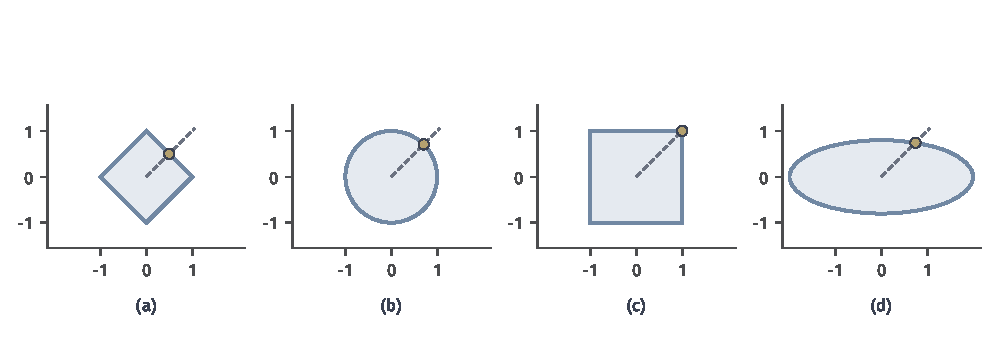
\includegraphics[width=169mm]{figures/00-shared/mathematical-preliminaries-upper/02-linear-spaces/matplotlib/ls-norm-unit-balls/ls-norm-unit-balls.pdf}
  \caption{三种范数的单位球。左：$\ell_1$单位球为菱形（累加绝对偏差）；中：$\ell_2$单位球为圆（欧氏长度）；右：$\ell_\infty$单位球为正方形（最大坐标偏差）。同一个点$(1,1)$的三种范数依次为$2$、$\sqrt2$、$1$。三者之间的倍数关系见第~\ref{sec:ls-error-scale-comparison}节。三图坐标尺度相同，为解析教学例。}
  \label{fig:ls-norm-unit-balls}
\end{figure*}

\subsubsection{范数的性质}
\label{sec:ls-p-norm-properties}

$1$、$2$、$\infty$范数的算法不同，却有几条共同的性质：大小非负，只有零向量的大小为零；向量放大$c$倍，大小变为$|c|$倍；两个向量之和的大小不超过各自大小之和。本小节对全部$p$范数证明这些性质，再比较不同$p$范数给出的大小最多相差多少倍。

\paragraph{非负性、正定性与齐次性}
这三条可以从公式直接读出。$\lVert\bm x\rVert_p$由绝对值汇总而成，总是非负；它为零当且仅当每个$|x_j|=0$，即$\bm x=\bm0$。

把$\bm x$换成$c\bm x$，每个$|x_j|$都乘以$|c|$。在$1\leq p<\infty$时，公式中的$p$次方与$1/p$次方相互抵消；在$p=\infty$时，最大值也乘以$|c|$。所以
\[
 \lVert c\bm x\rVert_p=|c|\,\lVert\bm x\rVert_p.
\]

\paragraph{三角不等式}
需要证明的只有三角不等式$\lVert\bm x+\bm y\rVert_p\leq\lVert\bm x\rVert_p+\lVert\bm y\rVert_p$。$p=1$和$p=\infty$时，它由实数的三角不等式逐坐标得到，见下面Minkowski不等式的证明。

$1<p<\infty$时，三角不等式要借助Hölder不等式。它用一对$p$范数与$q$范数控制两个向量逐坐标乘积之和，两个指数须满足共轭条件$1/p+1/q=1$。
\begin{theorem}[有限维Hölder不等式]
\label{thm:linear-algebra-holder}
设$\bm x,\bm y\in\mathbb R^d$，$1\leq p,q\leq\infty$且$1/p+1/q=1$（约定$1/\infty=0$），则
\begin{equation}
 |\bm x^\top\bm y|\leq\lVert\bm x\rVert_p\lVert\bm y\rVert_q.
 \label{eq:linear-algebra-holder}
\end{equation}
\end{theorem}
\begin{proof}
先设$1<p,q<\infty$，分三步证明。

第一步，证明Young不等式：对$u,v\geq0$，
\[
 uv\leq\frac{u^p}{p}+\frac{v^q}{q}.
\]
$u=0$时左侧为零，不等式成立。$u>0$时令$t=v/u^{p-1}\geq0$。由$1/p+1/q=1$得$(p-1)q=p$，于是
\[
 v^q=t^qu^{(p-1)q}=t^qu^p,\qquad uv=tu^p.
\]
代入后，不等式化为
\[
 u^p\Bigl(\frac1p+\frac{t^q}{q}-t\Bigr)\geq0.
\]
只需证明括号内的函数$f(t)=1/p+t^q/q-t$在$t\geq0$上非负。它的导数
\[
 f'(t)=t^{q-1}-1
\]
在$0<t<1$时为负、在$t>1$时为正，所以$f$在$t\geq0$上的最小值是
\[
 f(1)=\frac1p+\frac1q-1=0,
\]
不等式成立。

第二步，在单位尺度下求和。若$\bm x$或$\bm y$为零向量，结论两侧都为零。否则令$u_j=|x_j|/\lVert\bm x\rVert_p$、$v_j=|y_j|/\lVert\bm y\rVert_q$，则
\[
 \sum_ju_j^p=\sum_jv_j^q=1.
\]
对每个$j$用Young不等式再求和，得
\[
 \sum_ju_jv_j\leq\frac1p\sum_ju_j^p+\frac1q\sum_jv_j^q=\frac1p+\frac1q=1.
\]

第三步，恢复尺度。上式两边乘以$\lVert\bm x\rVert_p\lVert\bm y\rVert_q$，再用$|\bm x^\top\bm y|\leq\sum_j|x_j||y_j|$，即得
\[
 |\bm x^\top\bm y|\leq\sum_j|x_j||y_j|\leq\lVert\bm x\rVert_p\lVert\bm y\rVert_q.
\]

端点情形直接估计。$p=1$、$q=\infty$时，
\[
 \sum_j|x_j||y_j|\leq\Bigl(\max_j|y_j|\Bigr)\sum_j|x_j|=\lVert\bm x\rVert_1\lVert\bm y\rVert_\infty;
\]
$p=\infty$、$q=1$时交换两个向量的角色。
\end{proof}
$p=q=2$时，它给出$|\bm x^\top\bm y|\leq\lVert\bm x\rVert_2\lVert\bm y\rVert_2$。第~\ref{sec:ls-inner-product-definition}节将只用内积公理，对任一内积证明同样形式的不等式，即Cauchy--Schwarz不等式。

有了Hölder不等式，就可以对一般的$p$证明三角不等式。做法是把$|x_j+y_j|^p$拆成两个乘积之和，再对每一部分使用Hölder不等式。
\begin{theorem}[有限维Minkowski不等式]
\label{thm:linear-algebra-minkowski}
设$\bm x,\bm y\in\mathbb R^d$，$1\leq p\leq\infty$，则
\begin{equation}
 \lVert\bm x+\bm y\rVert_p\leq\lVert\bm x\rVert_p+\lVert\bm y\rVert_p.
 \label{eq:linear-algebra-minkowski}
\end{equation}
\end{theorem}
\begin{proof}
先处理两个端点。$p=1$时，对每个坐标使用实数的三角不等式，再求和，得到
\[
 \sum_j|x_j+y_j|\leq\sum_j|x_j|+\sum_j|y_j|.
\]
$p=\infty$时，对每个$j$都有
\[
 |x_j+y_j|\leq\lVert\bm x\rVert_\infty+\lVert\bm y\rVert_\infty.
\]
左侧对$j$取最大值，就得到所需结论。

下面设$1<p<\infty$。若$\bm x+\bm y=\bm0$，左侧为零，结论成立；以下设和向量非零。

取$q=p/(p-1)$，则$1/p+1/q=1$。先把每个坐标的$p$次方拆开，再用实数的三角不等式：
\[
 \begin{aligned}
 |x_j+y_j|^p
 &=|x_j+y_j|^{p-1}|x_j+y_j|\\
 &\leq |x_j+y_j|^{p-1}(|x_j|+|y_j|).
 \end{aligned}
\]
令$s_j=|x_j+y_j|^{p-1}$，把这些数排成向量$\bm s$。由于$(p-1)q=p$，它的$q$范数为
\[
 \begin{aligned}
 \lVert\bm s\rVert_q
 &=\Bigl(\sum_j|x_j+y_j|^p\Bigr)^{1/q}\\
 &=\lVert\bm x+\bm y\rVert_p^{p-1}.
 \end{aligned}
\]
把逐坐标的不等式求和，并对含$|x_j|$和含$|y_j|$的两部分分别使用Hölder不等式，得到
\[
 \begin{aligned}
 \lVert\bm x+\bm y\rVert_p^p
 &\leq\sum_js_j|x_j|+\sum_js_j|y_j|\\
 &\leq\lVert\bm s\rVert_q
       \bigl(\lVert\bm x\rVert_p+\lVert\bm y\rVert_p\bigr)\\
 &=\lVert\bm x+\bm y\rVert_p^{p-1}
       \bigl(\lVert\bm x\rVert_p+\lVert\bm y\rVert_p\bigr).
 \end{aligned}
\]
两边除以正数$\lVert\bm x+\bm y\rVert_p^{p-1}$，即得结论。
\end{proof}
所以每个$p$范数都满足三角不等式，特别是欧氏长度：两边之和不小于第三边。


\paragraph{范数的比较}
\phantomsection
\label{sec:ls-error-scale-comparison}

不同的$p$范数给同一个向量的大小不同。误差估计常常要在两种范数之间换算，因此需要知道它们最多相差多少倍。对$\mathbb R^d$中的坐标范数，这个倍数可以由有限求和直接算出。
\begin{theorem}[坐标范数的比较]
\label{thm:ls-coordinate-norm-comparison}
设$1\leq p\leq q\leq\infty$，约定$1/\infty=0$。对$\bm x\in\mathbb R^d$，
\begin{equation}
 \lVert\bm x\rVert_q\leq\lVert\bm x\rVert_p\leq d^{1/p-1/q}\lVert\bm x\rVert_q.
 \label{eq:ls-coordinate-norm-comparison}
\end{equation}
\end{theorem}
\begin{proof}
$\bm x=\bm0$时三项都为零，下设$\bm x\neq\bm0$。

左侧。令$\bm u=\bm x/\lVert\bm x\rVert_p$，则$\lVert\bm u\rVert_p=1$，所以每个$|u_j|\leq1$。$q=\infty$时这就是$\lVert\bm u\rVert_\infty\leq1$。

$q<\infty$时，由$|u_j|\leq1$与$q\geq p$得$|u_j|^q\leq|u_j|^p$。对$j$求和，得
\[
 \lVert\bm u\rVert_q^q\leq\lVert\bm u\rVert_p^p=1.
\]
两种情形都有$\lVert\bm u\rVert_q\leq1$，两边乘以$\lVert\bm x\rVert_p$即得。

右侧。$p=q$时两侧相同。$q=\infty$时，每一项$|x_j|^p$都不超过$\lVert\bm x\rVert_\infty^p$，于是
\[
 \sum_j|x_j|^p\leq d\,\lVert\bm x\rVert_\infty^p,
\]
开$p$次方即得。

设$p<q<\infty$，取$r=q/p>1$，其共轭指数满足$1/r'=1-p/q$。对向量$(|x_1|^p,\ldots,|x_d|^p)^\top$与全$1$向量使用Hölder不等式（定理~\ref{thm:linear-algebra-holder}），得
\[
 \begin{aligned}
 \sum_j|x_j|^p\cdot1
 &\leq\Bigl(\sum_j|x_j|^{q}\Bigr)^{p/q}d^{\,1-p/q}\\
 &=\lVert\bm x\rVert_q^p\,d^{\,1-p/q}.
 \end{aligned}
\]
两边开$p$次方，得
\[
 \lVert\bm x\rVert_p\leq d^{1/p-1/q}\lVert\bm x\rVert_q.
\]
\end{proof}
最常用的是$p,q\in\{1,2,\infty\}$的情形：
\[
 \begin{gathered}
 \lVert\bm x\rVert_\infty\leq\lVert\bm x\rVert_2\leq\sqrt d\,\lVert\bm x\rVert_\infty,\\
 \lVert\bm x\rVert_2\leq\lVert\bm x\rVert_1\leq\sqrt d\,\lVert\bm x\rVert_2,\\
 \lVert\bm x\rVert_\infty\leq\lVert\bm x\rVert_1\leq d\,\lVert\bm x\rVert_\infty.
 \end{gathered}
\]
下面在示例~\ref{ex:ls-p-norms}的向量上核对前两行。
\begin{example}[范数比较的数值核对]
\label{ex:ls-norm-comparison-check}
取$d=2$与$\bm x=(3,-4)^\top$。示例~\ref{ex:ls-p-norms}已经算出$\lVert\bm x\rVert_1=7$，$\lVert\bm x\rVert_2=5$，$\lVert\bm x\rVert_\infty=4$。代入前两行，比较常数分别为$\sqrt2$：
\[
 \begin{gathered}
 4\leq5\leq4\sqrt2\approx5.66,\\
 5\leq7\leq5\sqrt2\approx7.07.
 \end{gathered}
\]
四个不等式都成立，而且右侧的界离实际值不远。同一个误差$\bm x$在三种范数下读出$4$、$5$、$7$三个不同的数，比较定理保证的是这些读数之间的倍数不超过与维数有关的常数。
\end{example}
两侧的常数一般都不能改进，取等号的向量很简单。
\begin{example}[比较常数的取等]
\label{ex:ls-l1-linf-constants}
两个极端的向量分别使两侧取等号：只有一个非零坐标的$\bm e_1$，和各坐标一样大的全$1$向量$\bm 1$。

对每个$p$都有$\lVert\bm e_1\rVert_p=1$，所以$\bm e_1$使左侧取等号。

另一方面，全$1$向量的各范数为
\[
 \lVert\bm 1\rVert_p=d^{1/p}\quad(p<\infty),\qquad
 \lVert\bm 1\rVert_\infty=1.
\]
因此在约定$1/\infty=0$下总有
\[
 \lVert\bm 1\rVert_p=d^{1/p-1/q}\lVert\bm 1\rVert_q,
\]
右侧取等号。

大小全部集中在一个坐标上时，各范数读数相同；各坐标绝对值相等时，读数相差最大。例如$\ell_1$与$\ell_\infty$之间的常数$1$与$d$分别由$\bm e_1$和$\bm 1$达到，都不能改进。
\end{example}
右侧的常数随维数增长。维数较大时，换用范数带来的倍数差别不能在误差估计中忽略；固定维数下的比较式也不能当作对所有维数一致成立的界。

这里只比较了有明确公式的坐标范数。有限维空间上任意两个范数都只相差常数倍（定理~\ref{thm:ls-norm-equivalence}），这一结论的证明要用到闭有界集上连续函数的最值，在第~\ref{sec:multivariable-norm-equivalence}节给出。

本节建立了坐标向量的基本计算：加法、数乘与线性组合产生新的向量，欧氏内积把两个向量配成一个数，范数衡量向量的大小，满足非负性、正定性、齐次性与三角不等式，不同$p$范数之间只差与维数有关的常数倍。把若干向量并排放在一起，就得到下一节的矩阵。

% 矩阵一节：矩阵的表示与常见矩阵；加法与数乘、转置、矩阵与向量的乘积、矩阵乘法、逐项乘积（各自先定义、再整理性质）；初等行变换；逆矩阵；矩阵的幂。行列式、迹与Frobenius内积见下一节。

\section{矩阵}
\label{sec:ls-matrices}

一批样本的特征排成一张数表以后，常要对每个样本用同一组权重求加权和。矩阵就是这样的数表，矩阵乘法则一次写出这些加权和。

本节先规定矩阵的写法，再逐个讨论矩阵的运算，每种运算都先给定义、再整理性质。重点是矩阵乘法：它保留了实数乘法的结合律与分配律，却失去了交换律与消去律。最后三小节用乘法回答三个具体问题：怎样用可撤销的步骤化简矩阵，怎样撤销一次乘法，怎样记录同一矩阵的反复作用。

\subsection{矩阵的表示与常见矩阵}
\label{sec:ls-matrix-representation}

向量中的一个数用一个索引定位。数表中的一个数要由所在的行与列共同确定，需要两个索引。

\paragraph{矩阵、元素与形状}
$m$行$d$列的实数表称为矩阵（matrix），记为$\bm A\in\mathbb R^{m\times d}$。第$i$行、第$j$列的元素记为$\bm A_{i,j}$，不致混淆时也写作$a_{i,j}$。$m\times d$称为矩阵的形状，行数写在前，列数写在后。$\bm A_{i,:}$表示第$i$行，$\bm A_{:,j}$表示第$j$列，冒号表示取该方向上的全部位置；第$j$列是$m$维列向量，第$i$行是$d$维行向量。例如在
\[
 \bm A=\begin{bmatrix}1&2&3\\4&5&6\end{bmatrix}\in\mathbb R^{2\times3}
\]
中，$\bm A_{2,1}=4$，第一行$\bm A_{1,:}=\left[\begin{smallmatrix}1&2&3\end{smallmatrix}\right]$，第三列$\bm A_{:,3}=(3,6)^\top$。

两个矩阵相等，是指形状相同且每个对应元素相等。

只有一行的矩阵就是行向量，只有一列的矩阵就是列向量，所以向量可以看作矩阵的特例。

\paragraph{设计矩阵}
用矩阵记录数据时，通常让每行对应一个样本，每列对应一个特征，这样的矩阵称为设计矩阵。把示例~\ref{ex:ls-nearly-collinear-features}中的$\bm c_1,\bm c_2$并排作为两列，得到三个样本、两个特征的设计矩阵
\begin{equation}
\bm X_{\varepsilon}
 =\begin{bmatrix}\bm c_1&\bm c_2\end{bmatrix}
 =\begin{bmatrix}1&1\\1&1+\varepsilon\\1&1-\varepsilon\end{bmatrix},\qquad
 \bm c_2=\bm c_1+\varepsilon\bm q.
\label{eq:linear-algebra-nearly-collinear-design}
\end{equation}
后面各章反复用这个矩阵考察两列几乎相同时会出现什么问题。

\subsubsection{常见矩阵}
\label{sec:prelim-common-matrices}

有些矩阵的元素有固定的分布模式：大部分位置为零，或者关于主对角线对称。这些模式会让后面的运算大为简化。下面按元素的位置与取值逐类给出定义和例子；它们在矩阵乘法下呈现的固定模式，在第~\ref{sec:ls-common-matrix-products}节随乘法讨论。依赖内积的正交矩阵与正定矩阵在第~\ref{chap:normed-inner-product-spaces}章建立。

\paragraph{方阵}
行数等于列数的矩阵称为方阵（square matrix），$n\times n$方阵也称$n$阶方阵。位置$(i,i)$上的元素组成主对角线。例如
\[
 \begin{bmatrix}1&2\\3&4\end{bmatrix}
\]
是二阶方阵，主对角元素为$1$和$4$；$2\times3$矩阵不是方阵。下面的对角矩阵和三角矩阵都限定为方阵。

\paragraph{零矩阵}
全部元素都为$0$的矩阵称为零矩阵（zero matrix），记作$\bm0$。它不要求是方阵，需要时写明形状，例如
\[
 \bm0_{2\times3}=\begin{bmatrix}0&0&0\\0&0&0\end{bmatrix}.
\]

\paragraph{对角矩阵}
主对角线以外的元素都为$0$的方阵称为对角矩阵（diagonal matrix），记为$\operatorname{diag}(d_1,\ldots,d_n)$。主对角元素本身可以为$0$。例如
\[
\begin{gathered}
\operatorname{diag}(2,0)=\begin{bmatrix}2&0\\0&0\end{bmatrix},\\
\operatorname{diag}(1,-1,3)=\begin{bmatrix}1&0&0\\0&-1&0\\0&0&3\end{bmatrix}.
\end{gathered}
\]

\paragraph{单位矩阵}
主对角元素全为$1$的对角矩阵称为单位矩阵（identity matrix），记为$\bm I_n$；不必强调阶数时写作$\bm I$。它的第$j$列就是标准坐标向量$\bm e_j$。例如
\[
 \bm I_3=\begin{bmatrix}1&0&0\\0&1&0\\0&0&1\end{bmatrix}=\begin{bmatrix}\bm e_1&\bm e_2&\bm e_3\end{bmatrix}.
\]

\paragraph{上三角矩阵}
$i>j$时$\bm A_{i,j}=0$的方阵称为上三角矩阵（upper triangular matrix）。它的主对角线以下全为零，非零元素只可能出现在主对角线及其上方。例如
\[
 \begin{bmatrix}1&2&3\\0&4&5\\0&0&6\end{bmatrix}.
\]

\paragraph{下三角矩阵}
$i<j$时$\bm A_{i,j}=0$的方阵称为下三角矩阵（lower triangular matrix），它的主对角线以上全为零。例如
\[
 \begin{bmatrix}1&0&0\\2&3&0\\4&5&6\end{bmatrix}.
\]
对角矩阵既是上三角矩阵，也是下三角矩阵。

\paragraph{对称矩阵}
若方阵满足$\bm A_{i,j}=\bm A_{j,i}$对全部$i,j$成立，就称为对称矩阵（symmetric matrix）。它的元素关于主对角线镜像对称。定义转置以后，这个条件可以写作$\bm A^\top=\bm A$。例如
\[
\begin{bmatrix}1&2\\2&3\end{bmatrix},\qquad
\begin{bmatrix}4&-1&0\\-1&2&5\\0&5&1\end{bmatrix}.
\]
对角矩阵都是对称矩阵。

\paragraph{置换矩阵}
把单位矩阵的各列重新排列，得到的方阵称为置换矩阵（permutation matrix）。它的每行、每列恰有一个$1$，其余元素为$0$。例如
\[
\begin{bmatrix}0&1\\1&0\end{bmatrix}=\begin{bmatrix}\bm e_2&\bm e_1\end{bmatrix},\qquad
\begin{bmatrix}0&0&1\\1&0&0\\0&1&0\end{bmatrix}=\begin{bmatrix}\bm e_2&\bm e_3&\bm e_1\end{bmatrix}.
\]
定义矩阵乘法以后会看到，第一个矩阵乘在平面向量上，交换它的两个坐标。

\subsection{加法与数乘}
\label{sec:ls-matrix-addition-scaling}

矩阵的加法与数乘沿用向量的逐项规则。同形矩阵$\bm A,\bm B\in\mathbb R^{m\times n}$逐项相加减，数乘把每个元素乘以同一个实数$c$：
\[
 \begin{gathered}
(\bm A\pm\bm B)_{i,j}=a_{i,j}\pm b_{i,j},\\
(c\bm A)_{i,j}=ca_{i,j}.
 \end{gathered}
\]
结果的形状不变。下面是一组二阶矩阵的算例。
\begin{example}[矩阵的加法、减法与数乘]
\label{ex:ls-matrix-addition-scaling}
取
\[
\bm A=\begin{pmatrix}1&2\\3&4\end{pmatrix},\qquad
\bm B=\begin{pmatrix}0&1\\-1&2\end{pmatrix},\qquad
c=3.
\]
每个位置上的元素单独运算：
\[
\begin{gathered}
\bm A+\bm B=\begin{pmatrix}1&3\\2&6\end{pmatrix},\\
\bm A-\bm B=\begin{pmatrix}1&1\\4&2\end{pmatrix},\\
3\bm A=\begin{pmatrix}3&6\\9&12\end{pmatrix}.
\end{gathered}
\]
以$(2,1)$位置为例，$\bm A+\bm B$在这里是$3+(-1)=2$，$\bm A-\bm B$在这里是$3-(-1)=4$，都只用到$\bm A$与$\bm B$的$(2,1)$元。三个结果仍是$2\times2$矩阵，这和向量的逐坐标运算完全一样。
\end{example}
与向量一样，两个矩阵相加，要求形状相同、对应位置含义相同。$2\times3$矩阵与$3\times2$矩阵的元素个数相同，却不能相加。同形矩阵的线性组合按同样方式定义。

\subsubsection{加法与数乘的性质}
同形矩阵逐项相加与数乘，所以向量的八条规则在每个位置上照样成立。对同形矩阵$\bm A,\bm B,\bm C$和实数$a,b$，
\[
\begin{aligned}
 &\bm A+\bm B=\bm B+\bm A, && (\bm A+\bm B)+\bm C=\bm A+(\bm B+\bm C),\\
 &\bm A+\bm0=\bm A, && \bm A+(-\bm A)=\bm0,\\
 &a(b\bm A)=(ab)\bm A, && 1\bm A=\bm A,\\
 &(a+b)\bm A=a\bm A+b\bm A, && a(\bm A+\bm B)=a\bm A+a\bm B.
\end{aligned}
\]
每一条都可以在任一位置$(i,j)$上用实数运算直接验证。

\subsection{转置}
\label{sec:ls-matrix-transpose}

转置交换行与列：$\bm A\in\mathbb R^{m\times n}$的元素$a_{i,j}$原样搬到$\bm A^\top\in\mathbb R^{n\times m}$的位置$(j,i)$，
\[
 (\bm A^\top)_{j,i}=\bm A_{i,j}.
\]
形状随之交换，数值不变，原来的第$i$行成为第$i$列。把列向量看作$d\times1$矩阵，这一定义与上一节向量的转置一致。下面的例子显示行怎样变成列。
\begin{example}[转置一个$2\times3$矩阵]
\label{ex:ls-transpose-two-by-three}
把
\[
 \bm A=\begin{bmatrix}1&2&3\\4&5&6\end{bmatrix}\in\mathbb R^{2\times3}
\]
的每个$(i,j)$元搬到$(j,i)$位置，得到
\[
 \bm A^\top=\begin{bmatrix}1&4\\2&5\\3&6\end{bmatrix}\in\mathbb R^{3\times2}.
\]
$\bm A$的第一行$(1,2,3)$竖了起来，成为$\bm A^\top$的第一列；第二行$(4,5,6)$成为第二列。形状也随之由$2\times3$变为$3\times2$。
\end{example}

\subsubsection{转置的性质}

转置只改变元素的位置。下面两条说明它与加法、数乘的关系，以及转置两次的结果；它与矩阵乘积的关系要等定义了矩阵乘法以后，在第~\ref{sec:ls-reshaping}节讨论。

\paragraph{与加法、数乘交换}
\[
 \begin{gathered}
(\bm A+\bm B)^\top=\bm A^\top+\bm B^\top,\\
(c\bm A)^\top=c\bm A^\top.
 \end{gathered}
\]
转置只搬动元素，逐项运算的结果搬到新位置后不变。

\paragraph{转置的转置}
\[
 (\bm A^\top)^\top=\bm A.
\]
转置两次，$(i,j)$元先搬到$(j,i)$，再搬回$(i,j)$，每个元素回到原位。

\subsection{矩阵与向量的乘积}
\label{sec:prelim-matrix-records-prediction}

设$n$次观测的输入排成设计矩阵$\bm X\in\mathbb R^{n\times d}$，权重排成$\bm w\in\mathbb R^d$。线性预测对第$i$次观测计算加权和$\sum_j x_{i,j}w_j$，也就是$\bm X$的第$i$行与$\bm w$的内积。矩阵与向量的乘积把这$n$个加权和一次写出。对$\bm A\in\mathbb R^{m\times d}$与$\bm u\in\mathbb R^d$，$\bm A\bm u$是$m$维列向量，
\begin{equation}
(\bm A\bm u)_i=\sum_{j=1}^d\bm A_{i,j}u_j,\qquad i=1,\ldots,m.
\label{eq:prelim-matrix-prediction}
\end{equation}
这里矩阵的列数必须等于向量的维数。

同一个乘积可以按行算，也可以按列算，两者结果相同：
\begin{itemize}
 \item 按行算：输出的第$i$个坐标是第$i$行与$\bm u$的内积。
 \item 按列算：式~\eqref{eq:prelim-matrix-prediction}中，$u_j$乘的恰好是第$j$列的各个元素，所以
 \[
  \bm A\bm u=u_1\bm A_{:,1}+u_2\bm A_{:,2}+\cdots+u_d\bm A_{:,d},
 \]
 即乘积是矩阵各列以$u_j$为系数的线性组合。
\end{itemize}
按列算还说明，$\bm e_j$只有第$j$个系数为$1$，所以$\bm A\bm e_j=\bm A_{:,j}$：乘第$j$个标准坐标向量，就取出第$j$列。对贯穿例，按列算得$\bm X_\varepsilon\bm w=w_1\bm c_1+w_2\bm c_2$，预测是两个特征取值向量的线性组合。

下面用一个二阶例子核对两种算法给出同一结果。
\begin{example}[按行与按列计算矩阵与向量的乘积]
\label{ex:ls-matrix-vector-rows-columns}
取
\[
\bm A=\begin{bmatrix}2&1\\0&3\end{bmatrix},\qquad
\bm u=\begin{bmatrix}1\\1\end{bmatrix}.
\]
下面第一行算式按行算，每个坐标是$\bm A$的一行与$\bm u$的内积；第二行算式按列算，把$\bm A$的两列以$u_1=u_2=1$为系数组合起来：
\[
\begin{gathered}
\bm A\bm u
 =\begin{bmatrix}2\cdot1+1\cdot1\\0\cdot1+3\cdot1\end{bmatrix}
 =\begin{bmatrix}3\\3\end{bmatrix},\\
\bm A\bm u=1\begin{bmatrix}2\\0\end{bmatrix}+1\begin{bmatrix}1\\3\end{bmatrix}
 =\begin{bmatrix}3\\3\end{bmatrix}.
\end{gathered}
\]
两种算法都得到$(3,3)^\top$。按行算的每一项乘积，在按列算中也恰好出现一次，只是加起来的顺序不同。
\end{example}

用于数据时，一次矩阵与向量的乘积给出全部样本的预测。下面以一次函数为例。
\begin{example}[用矩阵与向量的乘积计算一次函数的取值与残差]
\label{ex:ls-affine-predictions}
设要在$x=1,2,3$三处计算一次函数$ax+b$的值。把三处的$x$排成第一列、再补上一列$1$，系数排成向量，即
\[
\bm X=\begin{pmatrix}1&1\\2&1\\3&1\end{pmatrix},\qquad
\bm w=\begin{pmatrix}a\\b\end{pmatrix}.
\]
按行算，
\[
 \bm X\bm w=\begin{pmatrix}1\cdot a+1\cdot b\\2\cdot a+1\cdot b\\3\cdot a+1\cdot b\end{pmatrix}=\begin{pmatrix}a+b\\2a+b\\3a+b\end{pmatrix}.
\]
$\bm X\bm w$的三个坐标正是三处的函数值；第二列全为$1$，使每行都加上同一个截距$b$。再把三处的观测输出排成$\bm y=(y_1,y_2,y_3)^\top$，全部残差就是$\bm X\bm w-\bm y$，平方误差总和写成
\[
 \sum_{i=1}^3\bigl(a\,i+b-y_i\bigr)^2
 =\lVert\bm X\bm w-\bm y\rVert_2^2.
\]
左侧逐处求函数值、减去观测、平方后相加；右侧把同样的计算写成残差向量长度的平方。

这里只用到乘积按行展开和长度的定义，与样本数、特征数无关。$n$个样本、$d$个特征时同样有
\[
 \sum_{i=1}^n\Bigl(\sum_{j=1}^d x_{i,j}w_j-y_i\Bigr)^2=\lVert\bm X\bm w-\bm y\rVert_2^2.
\]
于是一次矩阵与向量的乘积给出全部预测，平方误差总和则是残差向量长度的平方。
\end{example}

\subsection{矩阵乘法}
\label{sec:ls-matrix-operations}
\label{sec:ls-multiplication}
\label{sec:prelim-linear-actions-composition}

两次加权求和可能接连进行。设$\bm B\in\mathbb R^{d\times k}$，$\bm A\in\mathbb R^{m\times d}$。对$\bm x\in\mathbb R^k$，先算$\bm y=\bm B\bm x$，再算$\bm z=\bm A\bm y$。这就是两个映射的复合：$\bm x\mapsto\bm B\bm x$的输出$\bm y$恰好落在$\bm y\mapsto\bm A\bm y$的定义域$\mathbb R^d$中，复合映射把$\bm x$直接送到$\bm A(\bm B\bm x)$；映射复合的一般定义可参考\BookChapterRef{chap:sets-relations-maps}{卷一“集合、关系与映射”一章}。

逐坐标代入，再交换有限求和的次序，得到
\begin{equation}
 z_i=\sum_{\ell=1}^d a_{i,\ell}\sum_{j=1}^k b_{\ell,j}x_j
 =\sum_{j=1}^k\left(\sum_{\ell=1}^d a_{i,\ell}b_{\ell,j}\right)x_j.
 \label{eq:linear-algebra-matrix-product}
\end{equation}
可见$\bm z$仍是$\bm x$各坐标的加权和。把括号中的系数排成一张表，就得到矩阵乘法的定义。

对$\bm A\in\mathbb R^{m\times d}$与$\bm B\in\mathbb R^{d\times k}$，乘积$\bm A\bm B\in\mathbb R^{m\times k}$定义为
\begin{equation}
 (\bm A\bm B)_{i,j}=\sum_{\ell=1}^d\bm A_{i,\ell}\bm B_{\ell,j}.
 \label{eq:prelim-matrix-composition}
\end{equation}
左矩阵的列数必须等于右矩阵的行数。第$(i,j)$项取左矩阵的第$i$行与右矩阵的第$j$列，逐项相乘后相加。被求和掉的公共维数$d$，就是中间结果$\bm y$的维数。
$\bm B$只有一列时，式~\eqref{eq:prelim-matrix-composition}就是式~\eqref{eq:prelim-matrix-prediction}。两个向量的内积$\bm x^\top\bm y$是$1\times d$矩阵与$d\times1$矩阵的乘积，结果是$1\times1$矩阵，我们把它与其唯一的元素等同看待。

非方阵相乘时，写出每个因子的形状尤其有用。以$2\times3$矩阵乘$3\times2$矩阵为例，
\[
 \begin{aligned}
 &\begin{pmatrix}1&2&0\\0&1&3\end{pmatrix}
 \begin{pmatrix}1&0\\2&1\\1&-1\end{pmatrix}\\
 &=\begin{pmatrix}1\cdot1+2\cdot2+0\cdot1&1\cdot0+2\cdot1+0\cdot(-1)\\
 0\cdot1+1\cdot2+3\cdot1&0\cdot0+1\cdot1+3\cdot(-1)\end{pmatrix}\\
 &=\begin{pmatrix}5&2\\5&-2\end{pmatrix}.
 \end{aligned}
\]
左矩阵的列数与右矩阵的行数都是$3$，乘法有定义；输出保留左矩阵的$2$行和右矩阵的$2$列。若这两个数不相等，行与列就无法逐项配对。

\subsubsection{矩阵乘法的性质}
\label{sec:ls-matrix-operation-properties}

矩阵乘法保留了实数乘法的结合律和分配律，但一般不满足交换律和消去律。下面逐条核对，并检查每条规则对形状的要求。

\paragraph{单位乘}
\[
\bm I_m\bm A=\bm A=\bm A\bm I_d,\qquad
\bm A\in\mathbb R^{m\times d}.
\]
$\bm I_m$的第$i$行是$\bm e_i^\top$，它乘$\bm A$的第$j$列，取出$a_{i,j}$；右乘同理。单位矩阵在矩阵乘法中的作用，相当于数$1$在实数乘法中的作用。

\paragraph{零乘}
\[
 \bm0\bm A=\bm0,\qquad\bm A\bm0=\bm0.
\]
乘积的每个元素都是若干乘积之和。一个因子全为零时，每一项都为零。各个零矩阵的形状由相乘的另一个因子决定。

反过来不成立：由$\bm A\bm B=\bm0$不能推出$\bm A=\bm0$或$\bm B=\bm0$。下面是一个反例。
\begin{example}[反例：两个非零矩阵的乘积为零]
\label{ex:ls-zero-product-nonzero-factors}
两个二阶矩阵
\[
\bm A=\begin{bmatrix}1&0\\0&0\end{bmatrix},\qquad
\bm B=\begin{bmatrix}0&0\\1&0\end{bmatrix}
\]
各有一个非零元，都不是零矩阵。按定义相乘，
\[
 \bm A\bm B=\begin{bmatrix}1\cdot0+0\cdot1&1\cdot0+0\cdot0\\0\cdot0+0\cdot1&0\cdot0+0\cdot0\end{bmatrix}=\begin{bmatrix}0&0\\0&0\end{bmatrix}.
\]
四个元素全为零。可见两个非零因子的乘积可以是零矩阵，实数中“乘积为零则必有一个因子为零”的推理不能搬到矩阵上。
\end{example}
按列看可以说明原因。由乘积的元素公式，$\bm A\bm B$的第$j$列就是$\bm A$乘$\bm B$的第$j$列。所以$\bm A\bm B=\bm0$恰好意味着$\bm B$的每一列$\bm b$都满足$\bm A\bm b=\bm0$。上例中$\bm A$只保留第一个坐标、把第二个坐标清零；$\bm B$的第一列$(0,1)^\top$只有第二个坐标非零，第二列为零，于是两列都被$\bm A$清零。

\paragraph{结合律}
\[
 (\bm A\bm B)\bm C=\bm A(\bm B\bm C).
\]
按式~\eqref{eq:prelim-matrix-composition}展开，两边的第$(i,j)$项都是$\sum_k\sum_l a_{i,k}b_{k,l}c_{l,j}$，只是两个有限求和的次序不同。从映射的角度看，这就是复合的结合律：先作用$\bm C$、再作用$\bm B$、最后作用$\bm A$，无论先把哪两步合并，得到的都是同一个映射。取$\bm C$为列向量$\bm x$，得$(\bm A\bm B)\bm x=\bm A(\bm B\bm x)$：用乘积作用一次，等于先用$\bm B$、再用$\bm A$作用。这正是式~\eqref{eq:linear-algebra-matrix-product}引出乘法定义时的计算。有了结合律，多个形状相容的矩阵连乘时不必加括号。

\paragraph{分配律与数乘相容}
\[
 \begin{gathered}
\bm A(\bm B+\bm C)=\bm A\bm B+\bm A\bm C,\\
(\bm A+\bm B)\bm C=\bm A\bm C+\bm B\bm C,\\
c(\bm A\bm B)=(c\bm A)\bm B=\bm A(c\bm B).
 \end{gathered}
\]
逐项展开有限和即得。把右因子取为列向量，就得到矩阵与向量的乘积保持线性组合：
\begin{equation}
\bm A(a\bm u+b\bm v)=a\bm A\bm u+b\bm A\bm v,\qquad
\bm u,\bm v\in\mathbb R^d,\quad a,b\in\mathbb R.
\label{eq:prelim-matrix-linearity}
\end{equation}

由这一性质，函数$\bm u\mapsto\bm A\bm u$由它在$\bm e_1,\ldots,\bm e_d$上的输出完全确定。因为$\bm u=\sum_ju_j\bm e_j$，所以$\bm A\bm u=\sum_ju_j\bm A\bm e_j$，而这些输出$\bm A\bm e_j$就是$\bm A$的各列。第~\ref{chap:linear-representation}章把保持线性组合的函数称为线性映射，并说明每个这样的映射都能由一张矩阵记录。

\paragraph{分块乘法}
把矩阵按行、列切成尺寸相容的块，乘法公式对块照样成立。以$2\times2$分块为例，
\[
 \begin{bmatrix}\bm A_{1,1}&\bm A_{1,2}\\\bm A_{2,1}&\bm A_{2,2}\end{bmatrix}
 \begin{bmatrix}\bm B_{1,1}&\bm B_{1,2}\\\bm B_{2,1}&\bm B_{2,2}\end{bmatrix}
 =\begin{bmatrix}
  \bm A_{1,1}\bm B_{1,1}+\bm A_{1,2}\bm B_{2,1}&\bm A_{1,1}\bm B_{1,2}+\bm A_{1,2}\bm B_{2,2}\\
  \bm A_{2,1}\bm B_{1,1}+\bm A_{2,2}\bm B_{2,1}&\bm A_{2,1}\bm B_{1,2}+\bm A_{2,2}\bm B_{2,2}
 \end{bmatrix}.
\]
条件是每对相乘的块中，左块的列数等于右块的行数。理由如下：结果的每一块只用到左因子的一个行块和右因子的一个列块；式~\eqref{eq:prelim-matrix-composition}中对中间索引$\ell$的求和可以按列块分段进行，各段之和就是整段的和。块可以像数一样参与运算，只是块的次序不能交换。

把块分到最细，得到三种常用的特例。右因子按列分块，得$(\bm A\bm B)_{:,j}=\bm A\bm B_{:,j}$；左因子按行分块，得$(\bm A\bm B)_{i,:}=\bm A_{i,:}\bm B$；把中间维数$d$切成长度为$1$的$d$段，得到
\begin{equation}
 \bm A\bm B=\sum_{\ell=1}^d\bm A_{:,\ell}\bm B_{\ell,:},
 \label{eq:ls-product-outer-sum}
\end{equation}
其中一列$\bm A_{:,\ell}\in\mathbb R^{m\times1}$乘一行$\bm B_{\ell,:}\in\mathbb R^{1\times k}$，得到$(i,j)$元素为$a_{i,\ell}b_{\ell,j}$的$m\times k$矩阵。第~\ref{chap:matrix-approximation}章讨论低秩近似时，就从式~\eqref{eq:ls-product-outer-sum}出发。下面用一个二阶乘积核对这个公式。
\begin{example}[把乘积写成列乘行之和]
\label{ex:ls-product-as-outer-sum}
取
\[
\bm A=\begin{pmatrix}1&1\\0&1\end{pmatrix},\qquad
\bm B=\begin{pmatrix}1&0\\0&2\end{pmatrix}.
\]
$\bm A$的两列为$(1,0)^\top$与$(1,1)^\top$，$\bm B$的两行为$(1,0)$与$(0,2)$。把第$\ell$列与第$\ell$行配成一对相乘，再把两个结果相加：
\[
 \bm A\bm B=\begin{pmatrix}1\\0\end{pmatrix}\begin{pmatrix}1&0\end{pmatrix}+\begin{pmatrix}1\\1\end{pmatrix}\begin{pmatrix}0&2\end{pmatrix}
 =\begin{pmatrix}1&0\\0&0\end{pmatrix}+\begin{pmatrix}0&2\\0&2\end{pmatrix}=\begin{pmatrix}1&2\\0&2\end{pmatrix}.
\]
按式~\eqref{eq:prelim-matrix-composition}逐项计算$\bm A\bm B$，也得到同一个矩阵。两种算法的区别只在于：逐项计算先固定位置$(i,j)$、再对$\ell$求和，列乘行之和先固定$\ell$、一次写出所有位置上的贡献。
\end{example}

\paragraph{交换律不成立}
一般$\bm A\bm B\neq\bm B\bm A$。形状不同时，两个乘积不一定都有定义；即使两个因子是同阶方阵，两种次序的乘积也可能不同。下面是一个反例。
\begin{example}[反例：先交换再保留与先保留再交换]
\label{ex:ls-noncommuting-pair}
考虑两个作用很简单的二阶矩阵：$\bm P$只保留第一个坐标，$\bm S$交换两个坐标，
\[
\bm P=\begin{bmatrix}1&0\\0&0\end{bmatrix},\qquad
\bm S=\begin{bmatrix}0&1\\1&0\end{bmatrix}.
\]
按两种次序相乘，得到
\[
\bm P\bm S=\begin{bmatrix}0&1\\0&0\end{bmatrix},\qquad
\bm S\bm P=\begin{bmatrix}0&0\\1&0\end{bmatrix},
\]
所以$\bm P\bm S\neq\bm S\bm P$。看它们对$\bm u\in\mathbb R^2$的作用，差别的来源就清楚了：$\bm P\bm S\bm u=(u_2,0)^\top$是先交换、再保留第一个坐标，留下的是$u_2$；$\bm S\bm P\bm u=(0,u_1)^\top$是先保留、再交换，留下的是$u_1$，并且被移到了第二个位置。
\end{example}
书写$\bm A\bm B\bm x$时，作用顺序从右向左：先作用$\bm B$，后作用$\bm A$。

\paragraph{消去律不成立}
由$\bm A\bm B=\bm A\bm C$且$\bm A\neq\bm0$，不能推出$\bm B=\bm C$。原因是$\bm A\bm B=\bm A\bm C$等价于$\bm A(\bm B-\bm C)=\bm0$，而乘积为零推不出$\bm B-\bm C=\bm0$。下面用示例~\ref{ex:ls-zero-product-nonzero-factors}构造反例。
\begin{example}[反例：非零的左因子不能消去]
\label{ex:ls-cancellation-fails}
沿用示例~\ref{ex:ls-zero-product-nonzero-factors}中的
\[
\bm A=\begin{bmatrix}1&0\\0&0\end{bmatrix},\qquad
\bm B=\begin{bmatrix}0&0\\1&0\end{bmatrix},
\]
再取$\bm C=\bm0$。那个例子已经算出$\bm A\bm B=\bm0$，而零乘给出$\bm A\bm C=\bm0$，所以$\bm A\bm B=\bm A\bm C$。但$\bm B\neq\bm C$：尽管$\bm A\neq\bm0$，等式两边的$\bm A$也不能消去。
\end{example}
如果$\bm A$是可逆方阵（第~\ref{sec:prelim-inverse-matrices}节），在$\bm A\bm B=\bm A\bm C$两边左乘$\bm A^{-1}$，就得到$\bm B=\bm C$。所以可逆的左因子可以消去，一般的非零因子则不能。

\subsubsection{转置与乘积}
\label{sec:ls-reshaping}

第~\ref{sec:ls-matrix-transpose}节整理的转置性质只涉及加法、数乘和转置本身。乘法把左因子的行与右因子的列配对求和，而转置交换行与列，因此要单独考察乘积转置以后两个因子怎样排列。下面先给出这条规则，再看它在内积和对称性上的两个推论。

\paragraph{乘积的转置}
\[
 (\bm A\bm B)^\top=\bm B^\top\bm A^\top.
\]
乘积转置以后，因子的次序反过来。按元素公式，
\[
 \begin{aligned}
 \bigl((\bm A\bm B)^\top\bigr)_{i,j}
 &=(\bm A\bm B)_{j,i}\\
 &=\sum_\ell a_{j,\ell}b_{\ell,i}\\
 &=\sum_\ell(\bm B^\top)_{i,\ell}(\bm A^\top)_{\ell,j}\\
 &=(\bm B^\top\bm A^\top)_{i,j}.
 \end{aligned}
\]
多个因子时依次使用这条规则，得$(\bm A\bm B\bm C)^\top=\bm C^\top\bm B^\top\bm A^\top$。

\paragraph{内积中的转置}
\[
\langle\bm A\bm x,\bm y\rangle=\langle\bm x,\bm A^\top\bm y\rangle,\qquad
\bm A\in\mathbb R^{m\times d},\ \bm x\in\mathbb R^d,\ \bm y\in\mathbb R^m.
\]
由上一条，$(\bm A\bm x)^\top\bm y=\bm x^\top\bm A^\top\bm y$。所以在欧氏内积中，作用在左侧向量上的$\bm A$，可以改写成作用在右侧向量上的$\bm A^\top$。

\paragraph{$\bm A^\top\bm A$对称}
对任意矩阵$\bm A$，$\bm A^\top\bm A$与$\bm A\bm A^\top$都是对称矩阵。由乘积的转置，$(\bm A^\top\bm A)^\top=\bm A^\top(\bm A^\top)^\top=\bm A^\top\bm A$；另一个同理。下面直接算出一个$\bm A\bm A^\top$。
\begin{example}[计算$\bm A\bm A^\top$]
\label{ex:ls-gram-product-symmetric}
取
\[
 \bm A=\begin{bmatrix}1&2&3\\4&5&6\end{bmatrix}.
\]
$\bm A^\top$的第$j$列就是$\bm A$的第$j$行，所以$\bm A\bm A^\top$的$(i,j)$元是$\bm A$的第$i$行与第$j$行的内积：
\[
 \bm A\bm A^\top=\begin{bmatrix}1+4+9&4+10+18\\4+10+18&16+25+36\end{bmatrix}=\begin{bmatrix}14&32\\32&77\end{bmatrix}.
\]
$(1,2)$元与$(2,1)$元都是第一、二两行的内积$32$；内积与两行的先后无关，所以结果必然对称。对角元$14$、$77$则是两行各自长度的平方。
\end{example}

\subsubsection{常见矩阵的乘法}
\label{sec:ls-common-matrix-products}

第~\ref{sec:prelim-common-matrices}节的几类常见矩阵参与乘法时，结果有固定的模式。下面逐类说明。

\paragraph{对角矩阵的乘法}
设$\bm D=\operatorname{diag}(d_1,\ldots,d_n)$。左乘和右乘对角矩阵分别给出
\[
 \begin{gathered}
(\bm D\bm A)_{i,j}=d_i\bm A_{i,j},\\
(\bm A\bm D)_{i,j}=\bm A_{i,j}d_j.
 \end{gathered}
\]
乘积公式中，左乘时只剩$\ell=i$一项，右乘时只剩$\ell=j$一项。所以左乘对角矩阵缩放各行，右乘缩放各列。作用在向量上，$\bm D\bm u=(d_1u_1,\ldots,d_nu_n)^\top$是逐坐标缩放。两个对角矩阵相乘时，对角元逐个相乘：
\[
 \operatorname{diag}(d_1,\ldots,d_n)\operatorname{diag}(e_1,\ldots,e_n)=\operatorname{diag}(d_1e_1,\ldots,d_ne_n).
\]
因此对角矩阵之间可以交换次序。下面的例子比较左乘与右乘。
\begin{example}[左乘与右乘对角矩阵]
\label{ex:ls-diagonal-scaling}
取
\[
\bm D=\operatorname{diag}(2,3),\qquad
\bm A=\begin{bmatrix}1&2\\3&4\end{bmatrix},
\]
把$\bm D$分别放在$\bm A$的左边和右边：
\[
 \begin{aligned}
 \bm D\bm A&=\begin{bmatrix}2\cdot1&2\cdot2\\3\cdot3&3\cdot4\end{bmatrix}=\begin{bmatrix}2&4\\9&12\end{bmatrix},\\
 \bm A\bm D&=\begin{bmatrix}1\cdot2&2\cdot3\\3\cdot2&4\cdot3\end{bmatrix}=\begin{bmatrix}2&6\\6&12\end{bmatrix}.
 \end{aligned}
\]
左乘把第一、二行分别乘以$2$、$3$，右乘则把第一、二列分别乘以$2$、$3$。两个结果不同：对角矩阵彼此可以交换，与一般矩阵相乘时仍要区分左右。
\end{example}

\paragraph{三角矩阵的乘法}
若$\bm A,\bm B$都是$n$阶上三角矩阵，则$\bm A\bm B$也是上三角矩阵，并且
\[
 (\bm A\bm B)_{i,i}=\bm A_{i,i}\bm B_{i,i}.
\]
理由如下。在$(\bm A\bm B)_{i,j}=\sum_\ell\bm A_{i,\ell}\bm B_{\ell,j}$中，$\bm A_{i,\ell}$只在$\ell\geq i$时可能非零，$\bm B_{\ell,j}$只在$\ell\leq j$时可能非零，所以只有$i\leq\ell\leq j$的项可能非零。$i>j$时没有这样的$\ell$，乘积元素为零；$i=j$时只剩$\ell=i$一项。下三角矩阵同理：两个下三角矩阵的乘积仍是下三角矩阵，对角元逐个相乘。下面是一个二阶算例。
\begin{example}[两个上三角矩阵的乘积]
\label{ex:ls-upper-triangular-product}
取两个上三角矩阵
\[
\bm A=\begin{bmatrix}1&2\\0&3\end{bmatrix},\qquad
\bm B=\begin{bmatrix}4&5\\0&6\end{bmatrix}.
\]
它们的乘积为
\[
 \bm A\bm B=\begin{bmatrix}1\cdot4+2\cdot0&1\cdot5+2\cdot6\\0\cdot4+3\cdot0&0\cdot5+3\cdot6\end{bmatrix}=\begin{bmatrix}4&17\\0&18\end{bmatrix}.
\]
左下角的$0\cdot4+3\cdot0$中，每一项都有一个因子取自主对角线以下的零，所以乘积仍是上三角矩阵。对角元$4=1\cdot4$、$18=3\cdot6$只是两个因子对角元的乘积；右上角的$17$则同时用到了两个因子的非对角元，没有这样简单的规律。
\end{example}

\paragraph{置换矩阵的乘法}
设$\bm P=\left[\begin{smallmatrix}\bm e_{\sigma(1)}&\cdots&\bm e_{\sigma(n)}\end{smallmatrix}\right]$，其中$\sigma$是$\{1,\ldots,n\}$上的排列，则
\[
 \begin{gathered}
(\bm P\bm A)_{\sigma(i),:}=\bm A_{i,:},\\
(\bm A\bm P)_{:,j}=\bm A_{:,\sigma(j)}.
 \end{gathered}
\]
也就是说，左乘$\bm P$把$\bm A$的第$i$行移到第$\sigma(i)$行；右乘$\bm P$后，第$j$列取自$\bm A$的第$\sigma(j)$列。例如二阶置换矩阵
\[
 \begin{bmatrix}0&1\\1&0\end{bmatrix}
\]
左乘交换两行，右乘交换两列。

两个置换矩阵的乘积仍是置换矩阵。设$\bm P'$是另一个置换矩阵，则$\bm P'\bm P$的第$j$列是$\bm P'\bm e_{\sigma(j)}$，即$\bm P'$的第$\sigma(j)$列。不同的$j$取到$\bm P'$的不同列，所以$\bm P'\bm P$的各列是互不相同的标准坐标向量，它是单位矩阵各列的一种重排。

\paragraph{对称矩阵的乘积}
若$\bm A,\bm B$是同阶对称矩阵，则
\[
 (\bm A\bm B)^\top=\bm B^\top\bm A^\top=\bm B\bm A,
\]
所以$\bm A\bm B$对称当且仅当$\bm A\bm B=\bm B\bm A$。两个对称矩阵一般不交换，它们的乘积一般也不对称。下面是一个反例。
\begin{example}[反例：两个对称矩阵的乘积不对称]
\label{ex:ls-symmetric-product-not-symmetric}
取两个对称矩阵
\[
\bm A=\begin{bmatrix}1&1\\1&0\end{bmatrix},\qquad
\bm B=\operatorname{diag}(1,2).
\]
右乘对角矩阵$\bm B$相当于把$\bm A$的第二列乘以$2$，
\[
 \bm A\bm B=\begin{bmatrix}1\cdot1&1\cdot2\\1\cdot1&0\cdot2\end{bmatrix}=\begin{bmatrix}1&2\\1&0\end{bmatrix}.
\]
原来关于主对角线对称的两个$1$，只有右上角的一个被放大，于是$(\bm A\bm B)_{1,2}=2\neq1=(\bm A\bm B)_{2,1}$，乘积不对称。这与上面的判据一致：换成左乘，$\bm B$放大的是第二行，
\[
 \bm B\bm A=\begin{bmatrix}1&1\\2&0\end{bmatrix}\neq\bm A\bm B,
\]
两个因子不交换。
\end{example}

\subsection{逐项乘积}
\label{sec:ls-hadamard-product}

矩阵乘法对公共索引求和。另一种常用的“乘积”不对任何索引求和，只把两个同形数组在同一位置上的元素相乘。

设$\bm A,\bm B\in\mathbb R^{m\times n}$，它们的\term{逐元素乘积}（Hadamard product）记作$\bm A\odot\bm B$，
\begin{equation}
 (\bm A\odot\bm B)_{i,j}=a_{i,j}b_{i,j}.
 \label{eq:ls-hadamard}
\end{equation}
输出仍是$m\times n$矩阵。同维向量和更高阶的同形数组也按同样的方式逐项相乘。

对同样两个矩阵，两种乘积的结果完全不同。
\begin{example}[逐项乘积与矩阵乘积的对比]
\label{ex:ls-hadamard-vs-matrix-product}
取
\[
\bm A=\begin{bmatrix}1&2\\3&4\end{bmatrix},\qquad
\bm B=\begin{bmatrix}0&1\\1&0\end{bmatrix},
\]
其中$\bm B$是交换两个坐标的置换矩阵。分别计算两种乘积：
\[
 \begin{aligned}
 \bm A\odot\bm B&=\begin{bmatrix}1\cdot0&2\cdot1\\3\cdot1&4\cdot0\end{bmatrix}=\begin{bmatrix}0&2\\3&0\end{bmatrix},\\
 \bm A\bm B&=\begin{bmatrix}1\cdot0+2\cdot1&1\cdot1+2\cdot0\\3\cdot0+4\cdot1&3\cdot1+4\cdot0\end{bmatrix}=\begin{bmatrix}2&1\\4&3\end{bmatrix}.
 \end{aligned}
\]
逐项乘积保留$\bm A$在$\bm B$取$1$处的元素，把$\bm B$为零的位置置零；矩阵乘积则是右乘置换矩阵，交换了$\bm A$的两列。两个结果在每个位置上都不同。
\end{example}
固定一个掩码矩阵$\bm M$，运算$\bm X\mapsto\bm M\odot\bm X$把$\bm M$为零的位置置零，把其余位置按$\bm M$的元素缩放。因此逐项乘积适合表达“挑选或调制另一个数组”。

\subsubsection{逐项乘积的性质}

逐项乘积在每个位置上只是实数乘法，所以它的规则都可以逐个位置从实数运算推出。以下矩阵的形状都相同。

\paragraph{交换律}
\[
 \bm A\odot\bm B=\bm B\odot\bm A.
\]
式~\eqref{eq:ls-hadamard}右端是实数乘法，逐个位置验证即得。逐项乘积可交换，矩阵乘积不可交换，这再次说明两者是不同的运算。

\paragraph{结合律}
\[
 (\bm A\odot\bm B)\odot\bm C=\bm A\odot(\bm B\odot\bm C),
\]
两边的$(i,j)$元素都是$a_{i,j}b_{i,j}c_{i,j}$。

\paragraph{分配律}
\[
 \bm A\odot(\bm B+\bm C)=\bm A\odot\bm B+\bm A\odot\bm C,
\]
两边的$(i,j)$元素都是$a_{i,j}(b_{i,j}+c_{i,j})$。

\paragraph{单位元是全$1$数组}
全部元素为$1$的同形数组$\bm J$满足$\bm J\odot\bm A=\bm A$。单位矩阵不是逐项乘积的单位元：$\bm I_2\odot\bm A$只保留$\bm A$的对角元，把非对角元都变为零。

\paragraph{对每个因子分别线性}
固定一个因子$\bm M$时，$\bm X\mapsto\bm M\odot\bm X$保持线性组合。两个因子都可变时，乘积只对每个因子分别线性，对两者整体不是线性的：同时把两个因子放大两倍，结果放大四倍。第~\ref{chap:linear-representation}章还会看到，换一组记录方向以后，矩阵乘积所表示的复合关系保持不变，逐项乘积的结果则随记录方式改变。

\subsection{初等行变换}
\label{sec:ls-elementary-row-operations}

解方程和求逆时，需要把一个矩阵逐步化成容易辨认的形式。每一步都应当可以撤销，这样才不会丢失原矩阵中的信息。为此，对矩阵的行只允许三种\term{初等行变换}（elementary row operation）。下面用$r_i$表示第$i$行，并用同一个矩阵
\[
 \bm A=\begin{bmatrix}1&2\\3&4\\5&6\end{bmatrix}
\]
分别演示。每种变换都可以写成左乘一个矩阵：对单位矩阵执行同一变换，所得矩阵称为\term{初等矩阵}（elementary matrix），记为$\bm E$，那么$\bm E\bm A$恰好是对$\bm A$执行这一变换的结果。

第一种是交换两行，记作$r_i\leftrightarrow r_k$。它只改变行的先后，不改变任何一行的内容。图~\ref{fig:ls-row-swap}交换$\bm A$的第$1$、$3$行，对应的初等矩阵是交换$\bm I_3$第$1$、$3$行所得的置换矩阵。再交换一次同样的两行，就回到原矩阵，所以这种变换的逆就是它自己。
\begin{figure}[!htb]
  \centering
  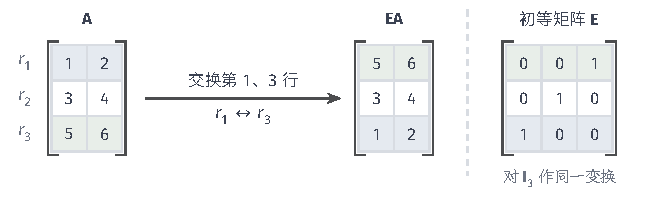
\includegraphics[width=109mm]{figures/02-vectors-matrices-and-multivariate-calculus/01-vectors-and-linear-spaces/tikz/ls-elementary-row-operations/row-swap.pdf}
  \caption{交换两行。左为$\bm A$，中间为交换第$1$、$3$行后的$\bm E\bm A$，右为对$\bm I_3$作同一交换得到的初等矩阵$\bm E$；同色表示同一行内容，换位后颜色随行移动。}
  \label{fig:ls-row-swap}
\end{figure}

第二种是将一行乘以非零数$c$，记作$r_i\leftarrow cr_i$。它把这一行的每个元素放大$c$倍，其余行不动。图~\ref{fig:ls-row-scale}把第$2$行乘以$2$，对应的初等矩阵是对角矩阵$\operatorname{diag}(1,2,1)$。要撤销它，只需把同一行乘以$1/c$。这里必须要求$c\neq0$：乘以$0$会把整行抹成零，原来的数据无法恢复。
\begin{figure}[!htb]
  \centering
  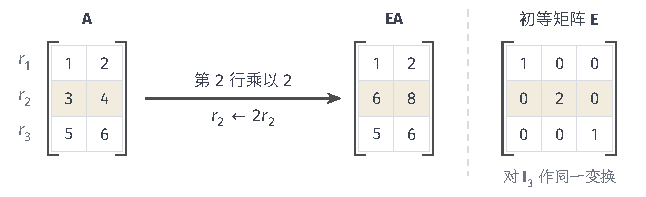
\includegraphics[width=109mm]{figures/02-vectors-matrices-and-multivariate-calculus/01-vectors-and-linear-spaces/tikz/ls-elementary-row-operations/row-scale.pdf}
  \caption{一行乘以非零数。第$2$行（黄色）乘以$2$，其余两行不变；初等矩阵$\bm E=\operatorname{diag}(1,2,1)$只在第$2$个对角元上与$\bm I_3$不同。}
  \label{fig:ls-row-scale}
\end{figure}

第三种是将一行加上另一行的倍数，记作$r_i\leftarrow r_i+cr_k$（$i\neq k$）。被加的一行改变，提供倍数的一行保持不动。图~\ref{fig:ls-row-replace}把第$3$行加上第$1$行的$-5$倍，第$3$行的首个元素$5$变成$0$；后面消元时正是用这种变换把指定位置化为零。对应的初等矩阵是在$\bm I_3$的$(3,1)$位置放上$-5$。撤销时，把第$3$行再加上第$1$行的$5$倍：第$1$行没有变，所以原来加上的量可以原样减回。
\begin{figure}[!htb]
  \centering
  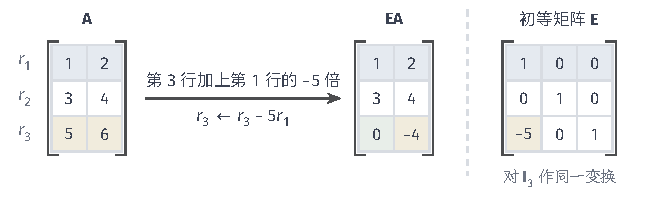
\includegraphics[width=109mm]{figures/02-vectors-matrices-and-multivariate-calculus/01-vectors-and-linear-spaces/tikz/ls-elementary-row-operations/row-replace.pdf}
  \caption{一行加上另一行的倍数。第$3$行（黄色）加上第$1$行（蓝色）的$-5$倍，第$1$行不变，第$3$行首个元素化为$0$（绿色）；初等矩阵$\bm E$只在$(3,1)$位置与$\bm I_3$不同。}
  \label{fig:ls-row-replace}
\end{figure}

三种变换的逆操作仍是同类的初等行变换，对应的初等矩阵就是$\bm E$的逆，所以每个初等矩阵都可逆。接连执行若干次行变换，相当于依次左乘这些初等矩阵，总的效果是左乘它们的乘积，它仍是可逆矩阵。

用初等行变换把矩阵化为阶梯形、求解线性方程组和求逆矩阵的具体做法，放在第~\ref{sec:ls-gaussian-elimination}节与求解方法一起讨论。

\subsection{逆矩阵}
\label{sec:prelim-inverse-matrices}

逆矩阵用来撤销一次矩阵乘法。对$n$阶方阵$\bm A$，若存在$n$阶方阵$\bm B$满足
\[
 \bm A\bm B=\bm B\bm A=\bm I_n,
\]
就称$\bm A$可逆，称$\bm B$为$\bm A$的\term{逆矩阵}（inverse matrix），记作$\bm A^{-1}$。

可逆矩阵给出的方程有唯一解。设$\bm A$可逆。若$\bm A\bm x=\bm y$，两边左乘$\bm A^{-1}$得$\bm x=\bm A^{-1}\bm y$，所以方程至多有一个解；反过来，$\bm x=\bm A^{-1}\bm y$满足$\bm A\bm x=\bm A\bm A^{-1}\bm y=\bm y$。所以方程$\bm A\bm x=\bm y$有唯一解$\bm x=\bm A^{-1}\bm y$。

逆矩阵若存在则唯一。若$\bm B,\bm C$都满足条件，由结合律，
\[
 \bm B=\bm B(\bm A\bm C)=(\bm B\bm A)\bm C=\bm C.
\]
因此记号$\bm A^{-1}$没有歧义。

怎样求逆取决于矩阵的结构。下面先给出对角矩阵和二阶方阵的逆，再说明一般方阵的求逆怎样归结为解方程。

\paragraph{对角矩阵的逆}
每个$d_i\neq0$时，逐个取倒数：
\[
 \operatorname{diag}(d_1,\ldots,d_n)^{-1}=\operatorname{diag}(1/d_1,\ldots,1/d_n).
\]
两个对角矩阵相乘时对角元逐个相乘，所以两侧乘积都是$\bm I_n$。例如$\operatorname{diag}(2,1)^{-1}=\operatorname{diag}(1/2,1)$。若某个$d_i=0$，则$\bm D=\operatorname{diag}(d_1,\ldots,d_n)$左乘任何$\bm B$，都把$\bm B$的第$i$行乘以$0$。于是$\bm D\bm B$的第$i$行是零，不可能等于$\bm I_n$的第$i$行，这时$\bm D$不可逆。

\paragraph{二阶方阵的逆}
$ad-bc\neq0$时，
\[
 \begin{pmatrix}a&b\\c&d\end{pmatrix}^{-1}=\frac1{ad-bc}\begin{pmatrix}d&-b\\-c&a\end{pmatrix}.
\]
直接相乘即可验证两侧乘积都是$\bm I_2$：例如左上元素为$(ad-bc)/(ad-bc)=1$，右上元素为$(-ab+ba)/(ad-bc)=0$。分母$ad-bc$就是下一节的二阶行列式。

\paragraph{一般方阵的逆}
一般方阵没有这样简短的公式。按列看等式$\bm A\bm A^{-1}=\bm I_n$，$\bm A^{-1}$的第$j$列$\bm A^{-1}\bm e_j$正是方程$\bm A\bm x=\bm e_j$的解，所以求逆就是解$n$个系数矩阵相同的线性方程组。怎样用初等行变换一并解这些方程，以及化简失败为什么说明矩阵不可逆，在第~\ref{sec:ls-gaussian-elimination}节讨论；方阵何时可逆，在第~\ref{chap:linear-solution-selection}章系统处理。只求一个方程的解时，通常直接消元或用分解求解，不必先求出整个逆矩阵。

\paragraph{单侧逆}
矩形矩阵没有双侧的逆，但可能从一侧抵消。对$\bm A\in\mathbb R^{m\times d}$，满足$\bm L\bm A=\bm I_d$的$\bm L\in\mathbb R^{d\times m}$称为左逆，满足$\bm A\bm R=\bm I_m$的$\bm R\in\mathbb R^{d\times m}$称为右逆。

两种单侧逆对方程$\bm A\bm x=\bm y$的作用不同。有左逆时，若方程有解，两边左乘$\bm L$得$\bm x=\bm L\bm y$，所以解只能是$\bm L\bm y$。有右逆时，$\bm A(\bm R\bm y)=\bm I_m\bm y=\bm y$，所以$\bm x=\bm R\bm y$总是一个解。

与方阵的逆不同，单侧逆一般不唯一。
\begin{example}[反例：左逆不唯一]
\label{ex:ls-left-inverse-not-unique}
取$\bm A=(1,0)^\top\in\mathbb R^{2\times1}$。对任意实数$c$，令$\bm L=(1,c)\in\mathbb R^{1\times2}$，则
\[
 \bm L\bm A=1\cdot1+c\cdot0=1=\bm I_1.
\]
$\bm A$的第二个坐标是零，$\bm L$的第二个元素无论取什么都不影响乘积。于是每个$c$都给出一个左逆，$\bm A$的左逆有无穷多个。
\end{example}

回到方阵。下面几条规则说明，可逆方阵经过乘积、求逆、数乘和转置以后仍然可逆，并给出逆矩阵的表达式。设$\bm A,\bm B$都是$n$阶可逆方阵。

\paragraph{乘积的逆}
两个可逆方阵的乘积仍然可逆，它的逆是两个因子的逆按相反次序相乘。
\begin{theorem}[乘积的逆]
\label{thm:ls-inverse-product}
设$\bm A,\bm B$都是$n$阶可逆方阵，则$\bm A\bm B$可逆，且
\begin{equation}
 (\bm A\bm B)^{-1}=\bm B^{-1}\bm A^{-1}.
 \label{eq:ls-inverse-product}
\end{equation}
\end{theorem}
\begin{proof}
由矩阵乘法的结合律，
\[
 \begin{gathered}
 (\bm A\bm B)(\bm B^{-1}\bm A^{-1})=\bm A(\bm B\bm B^{-1})\bm A^{-1}=\bm A\bm A^{-1}=\bm I_n,\\
 (\bm B^{-1}\bm A^{-1})(\bm A\bm B)=\bm B^{-1}(\bm A^{-1}\bm A)\bm B=\bm B^{-1}\bm B=\bm I_n.
 \end{gathered}
\]
按逆矩阵的定义，$\bm B^{-1}\bm A^{-1}$是$\bm A\bm B$的逆；由逆矩阵的唯一性，式~\eqref{eq:ls-inverse-product}成立。
\end{proof}
次序反转是因为$\bm A\bm B\bm x$先作用$\bm B$、再作用$\bm A$，撤销时要先撤销后作用的$\bm A$，再撤销$\bm B$。

\paragraph{逆的逆}
\[
 (\bm A^{-1})^{-1}=\bm A.
\]
在定义中，$\bm A$与$\bm A^{-1}$的地位对称：$\bm A^{-1}\bm A=\bm A\bm A^{-1}=\bm I_n$同样说明$\bm A$是$\bm A^{-1}$的逆。

\paragraph{数乘的逆}
\[
 (c\bm A)^{-1}=c^{-1}\bm A^{-1}\qquad(c\neq0).
\]
直接相乘：$(c\bm A)(c^{-1}\bm A^{-1})=(cc^{-1})\bm A\bm A^{-1}=\bm I_n$，反方向同理。

\paragraph{转置的逆}
\[
 (\bm A^\top)^{-1}=(\bm A^{-1})^\top.
\]
由乘积的转置，$\bm A^\top(\bm A^{-1})^\top=(\bm A^{-1}\bm A)^\top=\bm I^\top=\bm I$，反方向同理，所以$(\bm A^{-1})^\top$就是$\bm A^\top$的逆。

\subsection{矩阵的幂}
\label{sec:ls-matrix-power-rules}

同一个方阵反复作用，就得到矩阵的幂。对$d$阶方阵$\bm A$，$\bm A^k$定义为$k$个$\bm A$连乘（$k\geq1$），并规定$\bm A^0=\bm I_d$。$\bm A$可逆时，再定义负幂$\bm A^{-k}=(\bm A^{-1})^k$。非方阵不能与自身相乘，所以没有矩阵幂。

矩阵的幂是反复的矩阵乘法，不是逐元素乘方。下面的例子说明两者的差别。
\begin{example}[矩阵的平方不是逐元素平方]
\label{ex:ls-matrix-square-shear}
取
\[
 \bm A=\begin{pmatrix}1&1\\0&1\end{pmatrix},
\]
按矩阵乘法计算它的平方：
\[
 \bm A^2=\begin{pmatrix}1&1\\0&1\end{pmatrix}\begin{pmatrix}1&1\\0&1\end{pmatrix}
 =\begin{pmatrix}1\cdot1+1\cdot0&1\cdot1+1\cdot1\\0\cdot1+1\cdot0&0\cdot1+1\cdot1\end{pmatrix}
 =\begin{pmatrix}1&2\\0&1\end{pmatrix}.
\]
右上角的元素变为$2$，逐元素平方却只会得到$1^2=1$。差别在于$\bm A^2$的右上角是第一行与第二列的内积$1\cdot1+1\cdot1$，同时用到了两个元素。继续相乘，右上角每次增加$1$。
\end{example}

有两类矩阵由幂的关系刻画。满足$\bm A^2=\bm A$的方阵称为\term{幂等}（idempotent）矩阵，它作用一次与作用多次效果相同。存在正整数$s$使$\bm N^s=\bm0$的方阵称为\term{幂零}（nilpotent）矩阵。下面各举一例。
\begin{example}[幂等矩阵与幂零矩阵]
\label{ex:ls-idempotent-nilpotent}
看两个二阶矩阵
\[
\bm P=\operatorname{diag}(1,0),\qquad
\bm N=\begin{pmatrix}0&1\\0&0\end{pmatrix}
\]
对$\bm u\in\mathbb R^2$的作用。$\bm P\bm u=(u_1,0)^\top$只保留第一个坐标；$(u_1,0)^\top$再经过$\bm P$，第一个坐标照样保留，第二个坐标本来就是零，结果不变，所以$\bm P^2=\bm P$。$\bm N\bm u=(u_2,0)^\top$把第二个坐标移到第一个位置，并把第二个位置清零；再作用一次时，$\bm N$丢掉第一个坐标$u_2$，而第二个坐标已是零，得$\bm N(u_2,0)^\top=(0,0)^\top$。直接相乘也得到
\[
 \bm N^2=\begin{pmatrix}0&1\\0&0\end{pmatrix}\begin{pmatrix}0&1\\0&0\end{pmatrix}=\begin{pmatrix}0&0\\0&0\end{pmatrix}.
\]
所以$\bm P$是幂等矩阵；$\bm N$本身不是零矩阵，平方却为零，是幂零矩阵。
\end{example}

\subsubsection{幂的性质}
同一矩阵的幂按结合律满足与实数幂相同的指数法则。设$\bm A$为方阵，$m,n$为非负整数；$\bm A$可逆时，$m,n$可取任意整数。

\paragraph{同底幂相乘}
\[
 \bm A^m\bm A^n=\bm A^{m+n}.
\]
由结合律，两边都是同样个数的$\bm A$（或$\bm A^{-1}$）连乘；指数异号时，相邻的$\bm A\bm A^{-1}$逐对消去。交换$m,n$可见，同一矩阵的不同次幂彼此可以交换。不同矩阵则不一定交换，因此
\[
 (\bm A+\bm B)^2=\bm A^2+\bm A\bm B+\bm B\bm A+\bm B^2,
\]
只有$\bm A\bm B=\bm B\bm A$时，才能把中间两项合成$2\bm A\bm B$。这与标量平方公式的差别来自乘法的次序。

\paragraph{幂的幂}
\[
 (\bm A^m)^n=\bm A^{mn}.
\]
左边是$n$组、每组$m$个因子的连乘，由结合律去掉括号即得。

\paragraph{负幂与逆相容}
\[
 (\bm A^k)^{-1}=(\bm A^{-1})^k=\bm A^{-k}.
\]
对$k$个相同因子反复使用式~\eqref{eq:ls-inverse-product}即得。

% 方阵和同形矩阵的标量读数：行列式、迹与元素内积。
\section{行列式、迹与元素内积}
\label{sec:ls-matrix-scalar-readouts}

上一节的运算大多把矩阵变成另一个矩阵。本节讨论三种把矩阵变成一个数的运算：行列式衡量方阵对有向体积的缩放，迹累加主对角元素，Frobenius内积把两个同形矩阵的对应元素配对。三者回答的问题不同，单凭其中一个数也无法恢复原矩阵。

\subsection{行列式}
\phantomsection
\label{sec:ls-exterior-determinants}
\label{sec:linear-algebra-scalar-readouts}
\label{sec:ls-determinant-properties}
\label{sec:prelim-determinants}

行列式把一个方阵变成一个数。本小节先给出计算公式，再说明这个数度量有向体积的缩放，然后整理它的性质，最后用代数余子式构造古典伴随，并证明方阵的单侧逆就是逆。

\subsubsection{行列式的定义}

行列式的公式是对全部排列求和，所以先规定排列的符号。$\{1,\ldots,d\}$到自身的双射称为排列，全体排列记为$S_d$，共$d!$个。对排列$\pi$，满足$i<j$而$\pi(i)>\pi(j)$的索引对$(i,j)$称为逆序对，逆序对的个数记为$N(\pi)$。$\pi$的符号定义为$\operatorname{sgn}(\pi)=(-1)^{N(\pi)}$。
\begin{definition}[行列式]
\label{def:ls-determinant}
$d$阶方阵$\bm A=(a_{i,j})$的\term{行列式}（determinant）为
\[
 \det\bm A
 =\sum_{\pi\in S_d}\operatorname{sgn}(\pi)
   \prod_{i=1}^d a_{i,\pi(i)}.
\]
\end{definition}
每个排列$\pi$规定第$i$行取第$\pi(i)$列的元素。于是每一项从每行各取一个元素，各列也恰好各取一次；把取出的$d$个数相乘，按逆序对数的奇偶配上正负号，再对全部排列求和。可见行列式是矩阵元素的多项式。

同一个和也可以按列书写。把每项的乘积按列号重排，得$\prod_ia_{i,\pi(i)}=\prod_ja_{\pi^{-1}(j),j}$。$\pi$的逆序对$(i,j)$与$\pi^{-1}$的逆序对$(\pi(j),\pi(i))$一一对应，所以$\operatorname{sgn}(\pi^{-1})=\operatorname{sgn}(\pi)$。$\pi$遍历$S_d$时，$\sigma=\pi^{-1}$也遍历$S_d$，于是
\begin{equation}
 \det\bm A=\sum_{\sigma\in S_d}\operatorname{sgn}(\sigma)\prod_{j=1}^d a_{\sigma(j),j}.
 \label{eq:ls-det-column-form}
\end{equation}

二阶时只有两个排列。恒等排列没有逆序对，取正号；交换$1,2$的排列有一个逆序对，取负号。于是
\[
 \det\begin{pmatrix}a&b\\c&d\end{pmatrix}=ad-bc,
\]
例如
\[
 \det\begin{pmatrix}1&2\\3&4\end{pmatrix}=1\cdot4-2\cdot3=-2.
\]

三阶时有六个排列。恒等排列与两个循环排列$(\pi(1),\pi(2),\pi(3))=(2,3,1)$、$(3,1,2)$的逆序对数为$0$或$2$，取正号；只交换两个位置的三个排列$(1,3,2)$、$(2,1,3)$、$(3,2,1)$的逆序对数为$1$或$3$，取负号。于是
\[
 \begin{aligned}
 \det\bm A={}&a_{1,1}a_{2,2}a_{3,3}+a_{1,2}a_{2,3}a_{3,1}+a_{1,3}a_{2,1}a_{3,2}\\
 &-a_{1,1}a_{2,3}a_{3,2}-a_{1,2}a_{2,1}a_{3,3}-a_{1,3}a_{2,2}a_{3,1}.
 \end{aligned}
\]
下面用这个公式计算一个具体的三阶行列式。
\begin{example}[三阶行列式的排列展开]
\label{ex:ls-det-three-by-three}
取
\[
 \bm A=\begin{pmatrix}2&0&1\\1&3&0\\0&1&1\end{pmatrix},
\]
按上式的六项次序代入元素：
\[
 \begin{aligned}
 \det\bm A&=2\cdot3\cdot1+0\cdot0\cdot0+1\cdot1\cdot1-2\cdot0\cdot1-0\cdot1\cdot1-1\cdot3\cdot0\\
 &=6+0+1-0-0-0=7.
 \end{aligned}
\]
所以$\det\bm A=7$。六项中只有两项非零，其余四项都至少取到一个零元素。矩阵中的零越多，排列展开中需要真正计算的项就越少。
\end{example}
高阶时排列有$d!$个，直接展开很费力；实际计算通常借助后面的性质和消元。

\subsubsection{行列式的几何意义}

排列公式本身看不出行列式度量什么。本小节从平行四边形的面积和平行六面体的体积出发，只用它们满足的几条几何规则，推出同一个公式。

\paragraph{有向面积}
平面上两个向量$\bm u,\bm v$张成一个平行四边形。给它的面积配上符号：从$\bm u$逆时针转到$\bm v$（转角小于$\pi$）时取正，顺时针时取负。记这个\term{有向面积}为$S(\bm u,\bm v)$。它满足三条规则。
\begin{itemize}
 \item 对每条边线性：以$\bm v$为底，面积等于底长乘以$\bm u$在$\bm v$的法方向上的有向高；有向高是$\bm u$在一个单位法向量上的分量，对$\bm u$线性。所以
 \[
  S(a\bm u+b\bm w,\bm v)=aS(\bm u,\bm v)+bS(\bm w,\bm v),
 \]
 对第二条边同理。
 \item 交换两边变号：交换$\bm u,\bm v$，转向反过来，面积不变，即$S(\bm v,\bm u)=-S(\bm u,\bm v)$。特别地，$S(\bm u,\bm u)=0$，共线的两条边张成退化的平行四边形。
 \item 单位正方形的面积为$1$：$S(\bm e_1,\bm e_2)=1$。
\end{itemize}
把$\bm u=u_1\bm e_1+u_2\bm e_2$、$\bm v=v_1\bm e_1+v_2\bm e_2$代入，按第一条规则展开成四项，再用后两条规则，
\[
 \begin{aligned}
 S(\bm u,\bm v)
 &=u_1v_1\underbrace{S(\bm e_1,\bm e_1)}_{0}+u_1v_2\underbrace{S(\bm e_1,\bm e_2)}_{1}
 +u_2v_1\underbrace{S(\bm e_2,\bm e_1)}_{-1}+u_2v_2\underbrace{S(\bm e_2,\bm e_2)}_{0}\\
 &=u_1v_2-u_2v_1.
 \end{aligned}
\]
这正是以$\bm u,\bm v$为列的二阶行列式。下面用三组向量观察有向面积的数值与符号。
\begin{example}[平面上的有向面积]
\label{ex:ls-oriented-area}
取$\bm u=(1,0)^\top$与$\bm v=(1,1)^\top$，先按$(\bm u,\bm v)$的次序计算，再交换成$(\bm v,\bm u)$；最后换成一对共线向量$(1,1)^\top$与$(2,2)^\top$。按公式$u_1v_2-u_2v_1$，三组依次得到
\[
 \begin{gathered}
1\cdot1-0\cdot1=1,\\
1\cdot0-1\cdot1=-1,\\
1\cdot2-1\cdot2=0.
 \end{gathered}
\]
第一组张成底为$1$、高为$1$的平行四边形，从$\bm u$逆时针转到$\bm v$，有向面积为$1$。交换次序后，平行四边形没有变，转向却反了过来，所以只有符号变负。共线的两个向量张成的平行四边形退化成线段，有向面积为$0$。
\end{example}

\paragraph{有向体积}
空间中三个向量$\bm u,\bm v,\bm w$张成一个平行六面体。按右手系取正、左手系取负，得到\term{有向体积}$V(\bm u,\bm v,\bm w)$。理由与平面相同：以$\bm v,\bm w$张成的面为底，体积等于底面积乘以$\bm u$的有向高，所以$V$对$\bm u$线性，对其余两条棱同理；交换任意两条棱，右手系变为左手系，$V$变号；单位立方体$V(\bm e_1,\bm e_2,\bm e_3)=1$。

把三条棱都按坐标展开，共得$3^3=27$项，每项形如$u_iv_jw_k\,V(\bm e_i,\bm e_j,\bm e_k)$。$i,j,k$中有两个相同时，交换这两个相同的向量不改变$V$，却又使它变号，所以这一项为零。

留下的六项中$(i,j,k)$是$(1,2,3)$的排列$\sigma$。把$\bm e_{\sigma(1)},\bm e_{\sigma(2)},\bm e_{\sigma(3)}$排回原来的次序时，每交换一对相邻且次序颠倒的向量，逆序对数恰好减少$1$，所以恰好交换$N(\sigma)$次，$V(\bm e_{\sigma(1)},\bm e_{\sigma(2)},\bm e_{\sigma(3)})=\operatorname{sgn}(\sigma)$。于是
\[
 V(\bm u,\bm v,\bm w)=\sum_{\sigma\in S_3}\operatorname{sgn}(\sigma)\,u_{\sigma(1)}v_{\sigma(2)}w_{\sigma(3)},
\]
即式~\eqref{eq:ls-det-column-form}在$d=3$时的形式：$V(\bm u,\bm v,\bm w)=\det[\bm u\ \bm v\ \bm w]$。

\paragraph{一般维数}
上面的展开只用到两条规则：对每个向量线性，交换两个向量变号。$d$维时照样展开，得到下面的结论：设$D$把$d$个$\mathbb R^d$中的向量映成一个数，对每个向量线性，并且交换任意两个向量时变号，则
\begin{equation}
 D(\bm a_1,\ldots,\bm a_d)=D(\bm e_1,\ldots,\bm e_d)\,\det\begin{bmatrix}\bm a_1&\cdots&\bm a_d\end{bmatrix}.
 \label{eq:ls-det-volume}
\end{equation}
反过来也可以直接验证，排列公式作为各列的函数确实满足这两条规则：它对每列线性；交换两列相当于把每个排列复合一次对换，逆序对数的奇偶随之改变。所以行列式就是满足两条规则、并在单位矩阵处取值$1$的那个函数。

把$d$维平行多面体的有向体积取作$D$，单位立方体的体积为$1$，代入$\bm a_j=\bm A\bm e_j$，得到：$\det\bm A$是$\bm A$的各列张成的平行多面体的有向体积。$\bm A$把单位立方体映成这个平行多面体，所以$\det\bm A$是$\bm A$作用下有向体积的放大倍数：绝对值是体积之比，符号表示定向是否翻转。图~\ref{fig:ls-determinant-oriented-volume}画出了平面上的这种缩放。
\begin{figure*}[htbp]
  \centering
  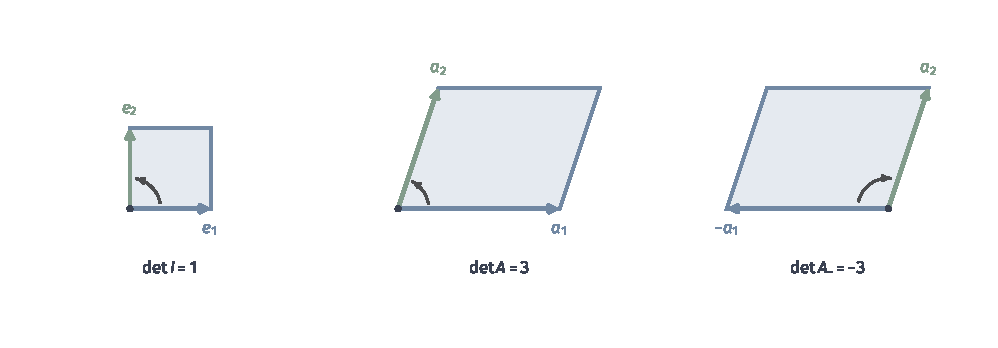
\includegraphics[width=169mm]{figures/00-shared/mathematical-preliminaries-upper/02-linear-spaces/matplotlib/ls-determinant-oriented-volume/ls-determinant-oriented-volume.pdf}
  \caption{行列式作为有向体积的缩放。左：单位正方形由$\bm e_1=(1,0)$、$\bm e_2=(0,1)$张成，面积为$1$。中：$\bm A=\bigl(\begin{smallmatrix}2&0.5\\0&1.5\end{smallmatrix}\bigr)$把它映成由$\bm A\bm e_1=(2,0)$、$\bm A\bm e_2=(0.5,1.5)$张成的平行四边形，有向面积为$2\cdot1.5-0.5\cdot0=3=\det\bm A>0$（保定向）。右：$\bm A$把$\bm e_1$反射到$(-2,0)$，有向面积为$-3$（反定向）。向量与数值均为解析教学例。}
  \label{fig:ls-determinant-oriented-volume}
\end{figure*}

\subsubsection{行列式的性质}

上一小节表明，行列式是各列张成的有向体积。下面的前两条性质就是有向体积的两条规则，其余性质由它们和排列公式推出。设$\bm A,\bm B$为$d$阶方阵。

\paragraph{对列的多线性}
三个矩阵只在同一列上不同、其余各列相同时，
\[
 \det\begin{bmatrix}\cdots&a\bm u+b\bm w&\cdots\end{bmatrix}
 =a\det\begin{bmatrix}\cdots&\bm u&\cdots\end{bmatrix}
 +b\det\begin{bmatrix}\cdots&\bm w&\cdots\end{bmatrix}.
\]

\paragraph{交替性}
交换两列，行列式变号；两列相同，行列式为零。前者是有向体积的规则，也已由排列公式验证。后者是因为交换两个相同的列不改变矩阵，行列式却要变号。

由多线性和交替性还能得到两个常用结论。第一，把某列的倍数加到另一列上，行列式不变：按多线性拆开后，多出的一项有两列相同，等于零。第二，某一列是其余各列的线性组合时，行列式为零：把这一列按组合展开，每一项都有两列相同。例如第二列是第一列的$2$倍时，
\[
 \det\begin{pmatrix}1&2\\2&4\end{pmatrix}=4-4=0.
\]

\paragraph{行变换与可逆性}
列上的这两条规则对行同样成立。排列公式的每一项从每行恰取一个元素，所以行列式对每一行也是线性的。交换第$i,k$两行，相当于把每个$\pi$与交换$i,k$的对换复合，逆序对数的奇偶随之改变，所以行列式变号。于是三种初等行变换对行列式的影响为：
\[
 \begin{aligned}
 &\text{交换两行：}&&\text{行列式变号；}\\
 &\text{某行乘以非零数}c\text{：}&&\text{行列式乘以}c\text{；}\\
 &\text{某行加上另一行的倍数：}&&\text{行列式不变。}
 \end{aligned}
\]

每一步消元都只使行列式乘以一个非零数，所以消元前后行列式是否为零不变。若某列找不到主元，阶梯形至少有一行全零；由对这一行的线性，行列式为零，矩阵也无法化为单位矩阵。若每列都找到主元，继续消元可以化为单位矩阵，而排列公式中$\det\bm I$只剩恒等排列一项，等于$1$，所以原矩阵的行列式非零，并且可以用第~\ref{sec:prelim-inverse-matrices}节的增广矩阵方法求逆。因此
\[
 \bm A\text{可逆}\iff\det\bm A\neq0.
\]

\paragraph{转置}
\[
 \det(\bm A^\top)=\det\bm A.
\]
$\bm A^\top$的排列公式为$\sum_\sigma\operatorname{sgn}(\sigma)\prod_j(\bm A^\top)_{j,\sigma(j)}=\sum_\sigma\operatorname{sgn}(\sigma)\prod_ja_{\sigma(j),j}$，这正是式~\eqref{eq:ls-det-column-form}。行列式对行和对列的性质因此完全对称。

\paragraph{数乘与加法}
\[
\begin{gathered}
\det(c\bm A)=c^d\det\bm A,\\
\det(\bm A+\bm B)\neq\det\bm A+\det\bm B\ (\text{一般}).
\end{gathered}
\]
数乘把$d$列各乘以$c$，由对每列的线性，提出$d$个$c$。行列式只对每一列分别线性，对整个矩阵却不是线性的。下面是一个反例。
\begin{example}[反例：行列式不保持加法]
\label{ex:ls-det-not-additive}
最简单的情形就足以说明问题。取$\bm A=\bm B=\bm I_2$，则$\det\bm A+\det\bm B=1+1=2$；而$\bm A+\bm B=2\bm I_2$，由上面的数乘公式，$\det(2\bm I_2)=2^2\det\bm I_2=4$。两者不等。原因在于两列同时加倍，体积要乘两次$2$。
\end{example}

\paragraph{乘法性}
\[
 \det(\bm A\bm B)=\det\bm A\,\det\bm B.
\]
从几何上看，接连作用两次，体积的放大倍数应当相乘。证明如下。固定$\bm A$，把$\det(\bm A\bm B)$看作$\bm B$的各列$\bm b_1,\ldots,\bm b_d$的函数
\[
 D(\bm b_1,\ldots,\bm b_d)=\det\begin{bmatrix}\bm A\bm b_1&\cdots&\bm A\bm b_d\end{bmatrix}=\det(\bm A\bm B).
\]
$\bm A\bm b_j$对$\bm b_j$线性，行列式对每列线性，所以$D$对每个$\bm b_j$线性；交换$\bm b_j,\bm b_k$就是交换$\bm A\bm B$的两列，$D$变号。由式~\eqref{eq:ls-det-volume}，
\[
 \det(\bm A\bm B)=D(\bm e_1,\ldots,\bm e_d)\det\bm B=\det\bm A\,\det\bm B.
\]
矩阵乘法不可交换，但$\det(\bm A\bm B)=\det(\bm B\bm A)$总成立，因为两边都等于$\det\bm A\,\det\bm B$。

\paragraph{三角矩阵的行列式}
\[
 \det\bm A=a_{1,1}a_{2,2}\cdots a_{d,d}\qquad(\bm A\text{为上三角或下三角矩阵}).
\]
设$\bm A$为上三角矩阵。若排列$\pi$不是恒等排列，必有某行$i$满足$\pi(i)<i$，因为$\sum_i(\pi(i)-i)=0$而各项不全为零。这一行取到主对角线下方的零元素，所以这一项为零，排列公式中只剩恒等排列一项。下三角时同理。例如
\[
 \det\begin{pmatrix}1&2&3\\0&4&5\\0&0&6\end{pmatrix}=1\cdot4\cdot6=24.
\]
特别地，$\det\operatorname{diag}(d_1,\ldots,d_d)=d_1\cdots d_d$。由乘法性，两个上三角矩阵乘积的行列式等于两者全部对角元之积，这与三角矩阵乘积的对角元逐个相乘一致。

结合行变换的规则，可以用消元计算行列式：先把方阵化为上三角矩阵，取对角元素的乘积，再补偿换行和倍乘的影响。例如
\[
 \det\begin{pmatrix}0&1&2\\1&2&1\\2&7&4\end{pmatrix}
 =-\det\begin{pmatrix}1&2&1\\0&1&2\\0&3&2\end{pmatrix}
 =-\det\begin{pmatrix}1&2&1\\0&1&2\\0&0&-4\end{pmatrix}=4.
\]
第一步交换前两行，并从第三行减去第一行的两倍；第二步从第三行减去第二行的三倍。交换行改变符号，两次加倍数不改变行列式。

\subsubsection{代数余子式与古典伴随}
\label{sec:ls-det-cofactor-adjugate}

排列公式有$d!$项。按某一行分组，可以把它化为$d$个$d-1$阶行列式。把这些低阶行列式排成矩阵，又能得到一个与$\bm A$相乘等于$(\det\bm A)\bm I_d$的矩阵。

\paragraph{按行（列）展开}
设$d\geq2$。删除第$i$行、第$j$列，得到的$(d-1)$阶子矩阵记为$\bm A^{(i,j)}$。定义\term{代数余子式}（cofactor）
\[
 C_{i,j}=(-1)^{i+j}\det\bm A^{(i,j)}.
\]
则对任一行$i$与任一列$j$，
\[
 \det\bm A=\sum_{j=1}^d a_{i,j}C_{i,j}=\sum_{i=1}^d a_{i,j}C_{i,j}.
\]
把排列公式按第$i$行所取的列分类，取第$j$列的各项之和正是$a_{i,j}C_{i,j}$；按列展开同理。下面沿第一行展开示例~\ref{ex:ls-det-three-by-three}中的矩阵，与排列公式的结果对照。
\begin{example}[沿第一行展开三阶行列式]
\label{ex:ls-det-cofactor-expansion}
仍取
\[
 \bm A=\begin{pmatrix}2&0&1\\1&3&0\\0&1&1\end{pmatrix}.
\]
第一行元素为$2,0,1$，对应代数余子式的符号$(-1)^{1+j}$依次为$+,-,+$。每个元素乘以删去它所在行、列后剩下的二阶行列式：
\[
 \begin{aligned}
 \det\bm A
 &=2\cdot\det\begin{pmatrix}3&0\\1&1\end{pmatrix}
 -0\cdot\det\begin{pmatrix}1&0\\0&1\end{pmatrix}
 +1\cdot\det\begin{pmatrix}1&3\\0&1\end{pmatrix}\\
 &=2\cdot3-0\cdot1+1\cdot1=7.
 \end{aligned}
\]
结果与示例~\ref{ex:ls-det-three-by-three}的排列展开一致。第一行的$0$使中间一项不必计算，所以按零较多的行或列展开最省事。
\end{example}

\paragraph{古典伴随恒等式}
把全部代数余子式排成矩阵$\bm C$，其转置$\operatorname{adj}(\bm A)=\bm C^\top$称为\term{古典伴随}（classical adjugate）。
\begin{theorem}[古典伴随恒等式]
\label{thm:ls-adjugate-identity}
对任意$d$阶方阵$\bm A$，
\[
 \bm A\,\operatorname{adj}(\bm A)
 =\operatorname{adj}(\bm A)\,\bm A
 =(\det\bm A)\,\bm I_d.
\]
\end{theorem}
\begin{proof}
乘积$\bm A\bm C^\top$的$(i,k)$元素为$\sum_j a_{i,j}C_{k,j}$。当$i=k$时，这正是沿第$i$行展开的$\det\bm A$。当$i\neq k$时，$C_{k,j}$不涉及第$k$行的元素，所以这个和是把第$k$行换成第$i$行后所得矩阵沿第$k$行的展开；新矩阵有两行相同，行列式为零。于是$\bm A\bm C^\top=(\det\bm A)\bm I_d$。按列展开，同样得到$\bm C^\top\bm A=(\det\bm A)\bm I_d$。
\end{proof}
二阶时
\[
 \operatorname{adj}\begin{pmatrix}a&b\\c&d\end{pmatrix}=\begin{pmatrix}d&-b\\-c&a\end{pmatrix},
\]
恒等式两边除以$ad-bc$，就是第~\ref{sec:prelim-inverse-matrices}节的二阶求逆公式。

古典伴随是由余子式得到的代数构造，与第~\ref{sec:ls-adjoints}节由内积定义的伴随不是同一个对象。高阶时展开余子式的代价是阶乘级的，所以这个恒等式主要用作证明工具。下面用它证明方阵的单侧逆即逆；后文还用它给出线性方程的可逆判据（第~\ref{sec:ls-determinant-invertibility}节），并证明Cayley--Hamilton定理（第~\ref{sec:ls-characteristic-polynomial}节）。

\paragraph{方阵的单侧逆即逆}
\phantomsection
\label{sec:ls-square-one-sided-inverse}
第~\ref{sec:prelim-inverse-matrices}节定义逆矩阵时，要求两侧乘积都等于单位矩阵。对方阵，一侧就够了。
\begin{theorem}[方阵的单侧逆即逆]
\label{thm:ls-square-one-sided-inverse}
设$\bm A,\bm B$为$n$阶方阵。若$\bm B\bm A=\bm I_n$或$\bm A\bm B=\bm I_n$，则$\bm A$可逆且$\bm B=\bm A^{-1}$。
\end{theorem}
\begin{proof}
由乘法性，两种情形都有$\det\bm A\det\bm B=\det\bm I_n=1$，所以$\det\bm A\neq0$。令$\bm C=\operatorname{adj}(\bm A)/\det\bm A$，由古典伴随恒等式，$\bm A\bm C=\bm C\bm A=\bm I_n$，所以$\bm A$可逆，且$\bm C=\bm A^{-1}$。若$\bm B\bm A=\bm I_n$，则$\bm B=\bm B(\bm A\bm C)=(\bm B\bm A)\bm C=\bm C$；若$\bm A\bm B=\bm I_n$，则$\bm B=(\bm C\bm A)\bm B=\bm C(\bm A\bm B)=\bm C$。
\end{proof}
所以检验方阵的逆，只需验证一侧的乘积。矩形矩阵则不同：左逆与右逆可以只存在一个，也可以不唯一（示例~\ref{ex:ls-left-inverse-not-unique}）。

\subsection{迹}
\label{sec:prelim-matrix-trace}

行列式要用到方阵的全部元素。迹只看主对角线：$n$阶方阵的\term{迹}（trace）是主对角元素之和，
\[
 \operatorname{tr}(\bm A)=\sum_{i=1}^n A_{i,i}.
\]
例如
\[
 \operatorname{tr}\begin{pmatrix}1&2\\3&4\end{pmatrix}=1+4=5,
\]
而这个矩阵全部元素之和是$10$。迹只对方阵定义，只累加对角元。

\subsubsection{迹的性质}
\phantomsection
\label{sec:ls-matrix-contractions}

迹是有限和，前两条性质可以直接看出；第三条循环性是迹最常用的性质。

\paragraph{线性}
\[
 \operatorname{tr}(a\bm A+b\bm B)=a\operatorname{tr}(\bm A)+b\operatorname{tr}(\bm B),
\]
这是有限和的线性。

\paragraph{转置不变}
\[
 \operatorname{tr}(\bm A^\top)=\operatorname{tr}(\bm A),
\]
因为转置不改变对角元。

\paragraph{循环性}
对$\bm A\in\mathbb R^{m\times n}$、$\bm B\in\mathbb R^{n\times m}$，
\begin{equation}
 \operatorname{tr}(\bm A\bm B)
 =\sum_{i=1}^m\sum_{j=1}^n A_{i,j}B_{j,i}
 =\operatorname{tr}(\bm B\bm A).
 \label{eq:linear-algebra-trace-cyclic}
\end{equation}
两个双重和只是求和次序不同。$\bm A\bm B$与$\bm B\bm A$可以是不同阶的方阵；相等的是它们的迹，不是矩阵本身。下面的例子说明这一点。
\begin{example}[不同阶乘积的迹相等]
\label{ex:ls-trace-cyclic-different-sizes}
取行向量$\bm A=\left[\begin{smallmatrix}1&2&3\end{smallmatrix}\right]\in\mathbb R^{1\times3}$与列向量$\bm B=(1,0,2)^\top\in\mathbb R^{3\times1}$。按“行乘列”的次序，$\bm A\bm B=1\cdot1+2\cdot0+3\cdot2=7$是$1\times1$矩阵；按“列乘行”的次序，
\[
 \bm B\bm A=\begin{bmatrix}1&2&3\\0&0&0\\2&4&6\end{bmatrix}
\]
是$3\times3$矩阵，对角元为$1,0,6$。两个乘积连阶数都不同，迹却相等：$\operatorname{tr}(\bm A\bm B)=7=1+0+6=\operatorname{tr}(\bm B\bm A)$。$\bm B\bm A$的对角元$A_{1,j}B_{j,1}$恰好是内积$\bm A\bm B$中的三项。
\end{example}

三个因子时，循环性只允许把因子整体循环移动：
\[
 \operatorname{tr}(\bm A\bm B\bm C)=\operatorname{tr}(\bm B\bm C\bm A)=\operatorname{tr}(\bm C\bm A\bm B).
\]
第一个等号把$\bm A$与$\bm B\bm C$看作两个因子，使用式~\eqref{eq:linear-algebra-trace-cyclic}；第二个等号把$\bm A\bm B$与$\bm C$看作两个因子。任意交换相邻因子则可能改变迹，下面是一个反例。
\begin{example}[反例：交换相邻因子会改变迹]
\label{ex:ls-trace-adjacent-swap}
取
\[
 \bm A=\begin{pmatrix}1&0\\0&0\end{pmatrix},\quad
 \bm B=\begin{pmatrix}0&0\\1&0\end{pmatrix},\quad
 \bm C=\begin{pmatrix}0&1\\0&0\end{pmatrix}.
\]
其中$\bm A,\bm B$就是示例~\ref{ex:ls-zero-product-nonzero-factors}中的两个矩阵，$\bm A\bm B=\bm0$，所以$\bm A\bm B\bm C=\bm0$。把$\bm B$与$\bm C$对调：$\bm C$的非零元在第一行，$\bm A$保留第一行，故$\bm A\bm C=\bm C$，从而
\[
 \bm A\bm C\bm B=\begin{pmatrix}0&1\\0&0\end{pmatrix}\begin{pmatrix}0&0\\1&0\end{pmatrix}=\begin{pmatrix}1&0\\0&0\end{pmatrix}.
\]
于是$\operatorname{tr}(\bm A\bm B\bm C)=0$，而$\operatorname{tr}(\bm A\bm C\bm B)=1$。$\bm A\bm C\bm B$不是$\bm A\bm B\bm C$的循环移动，迹可以不同。
\end{example}

\subsection{矩阵的元素内积}

行列式和迹都只对方阵定义，只用到一个矩阵。比较两个同形矩阵时，可以像向量内积那样，把全部对应元素配对。

\subsubsection{Frobenius内积}

把同形矩阵的$mn$个元素看作$mn$个坐标，照搬欧氏内积，就得到\term{Frobenius内积}：对$\bm A,\bm B\in\mathbb R^{m\times n}$，
\[
 \langle\bm A,\bm B\rangle_{\mathrm F}=\sum_{i=1}^m\sum_{j=1}^na_{i,j}b_{i,j}.
\]
它把对应元素逐项相乘后全部相加，也就是$\bm A\odot\bm B$全部元素之和。下面沿用逐项乘积一例中的两个矩阵。
\begin{example}[Frobenius内积的计算]
\label{ex:ls-frobenius-inner-product}
对
\[
 \bm A=\begin{pmatrix}1&2\\3&4\end{pmatrix},\quad
 \bm B=\begin{pmatrix}0&1\\1&0\end{pmatrix},
\]
按位置$(1,1),(1,2),(2,1),(2,2)$依次配对相乘再相加：
\[
 \langle\bm A,\bm B\rangle_{\mathrm F}=1\cdot0+2\cdot1+3\cdot1+4\cdot0=5.
\]
四个乘积正是示例~\ref{ex:ls-hadamard-vs-matrix-product}中$\bm A\odot\bm B$的四个元素$0,2,3,0$，所以Frobenius内积就是逐项乘积的元素之和。
\end{example}

\paragraph{Frobenius内积的迹表示}
Frobenius内积可以用迹写出：
\[
 \begin{gathered}
 \langle\bm A,\bm B\rangle_{\mathrm F}=\operatorname{tr}(\bm A^\top\bm B),\\
 \lVert\bm A\rVert_{\mathrm F}^2=\operatorname{tr}(\bm A^\top\bm A).
 \end{gathered}
\]
$\bm A^\top\bm B$的第$j$个对角元为$\sum_i A_{i,j}B_{i,j}$，再对$j$求和，恰好遍历所有位置。第二式中的$\lVert\bm A\rVert_{\mathrm F}$就是下面定义的Frobenius范数。反过来，计算$\operatorname{tr}(\bm A\bm B)$时也不必先求出乘积：只需计算$\sum_{i,j}A_{i,j}B_{j,i}$，代价为$mn$次乘法，而求出整个$\bm A\bm B$需要$m^2n$次。

\subsubsection{Frobenius范数}
\label{sec:ls-frobenius-norm}

由Frobenius内积可以定义矩阵的大小。把矩阵当作一张数表，定义Frobenius范数
\[
 \lVert\bm A\rVert_{\mathrm F}=\sqrt{\langle\bm A,\bm A\rangle_{\mathrm F}}=\left(\sum_{i,j}a_{i,j}^2\right)^{1/2}.
\]
例如
\[
 \left\lVert\begin{pmatrix}1&2\\3&4\end{pmatrix}\right\rVert_{\mathrm F}=\sqrt{1+4+9+16}=\sqrt{30}.
\]
它就是把$mn$个元素排成一列以后的$2$范数，其范数性质在第~\ref{sec:ls-normed-space-definition}节由Minkowski不等式统一验证。

Frobenius范数也可以从矩阵的作用来理解。由$\bm A\bm e_j=\bm A_{:,j}$，
\[
 \lVert\bm A\rVert_{\mathrm F}^2=\sum_j\lVert\bm A_{:,j}\rVert_2^2=\sum_j\lVert\bm A\bm e_j\rVert_2^2,
\]
即全部标准坐标向量输入后，输出长度的平方和。它不是某一个最坏输入的放大倍数；后者是另一种矩阵范数，在第~\ref{sec:ls-matrix-norms}节讨论。

数据按组划分时，还可以先在组内汇总、再汇总各组，得到混合范数。例如以行为组，$\lVert\bm A\rVert_{p,q}=(\sum_i\lVert\bm A_{i,:}\rVert_p^q)^{1/q}$：内层的$p$范数衡量每一行的大小，外层的$q$范数汇总各行。

% 第1章第4节：张量的表示（多维数组、轴、阶、形状、切片）；张量的重排（轴置换、形状重整与向量化及重排的性质）、张量积及其性质、Kronecker积及其性质、指标缩约及其性质。各种乘积的形状汇总见本章小结。

\section{张量}
\label{sec:ls-tensors-objects}

一批图像要记录样本、通道和两个像素坐标，一批文本要记录样本、位置和特征维度。定位其中一个数需要三个甚至更多的索引，一张矩阵装不下。本节先给出多维数组的记法，再按对轴的作用讨论三类运算：重排只改变元素所在的位置；张量积与Kronecker积把几个数组组合成轴更多的数组；缩约沿指定的轴求和，把数组汇总成轴更少的数组。每类运算之后整理它的性质。最后会看到，前两节的内积、矩阵乘法与迹都是缩约。

\subsection{张量的表示}
\label{sec:ls-tensor-representation}

向量用一个索引定位一个数，矩阵用两个。一个量由更多路索引共同决定时，就需要更多索引。机器学习中常把这样的多索引数值数组称为\term{张量}（tensor）。

数学中的“张量”还有不依赖坐标的定义，例如多线性映射或张量积空间的元素；本节只采用坐标数组的口径，把张量当作一张多索引的数表。数组与多线性映射的联系，在第~\ref{sec:ls-multilinear-maps}节选定基以后说明。
\begin{definition}[多维数值数组]
\label{def:linear-algebra-multidimensional-array}
给定正整数$n_1,\ldots,n_k$，形状为$n_1\times\cdots\times n_k$的数值数组，是从$\{1,\ldots,n_1\}\times\cdots\times\{1,\ldots,n_k\}$到$\mathbb R$的映射。第$j$个索引称为第$j$个\term{轴}（axis），轴数$k$称为数组的\term{阶}（order）。
\end{definition}
按这一定义，向量是一阶数组，矩阵是二阶数组；并约定单个标量是零阶数组。阶是索引的个数，形状记录各轴的长度。轴的长度再大也不改变阶：$\mathbb R^{100}$中的向量仍是一阶数组。

例如$\bm X\in\mathbb R^{b\times\ell\times d}$可以记录$b$个样本、每个样本$\ell$个位置、每个位置$d$个特征，元素$x_{i,j,k}$由三个索引共同定位。固定一部分索引，得到切片：$\bm X_{i,:,:}$保留第$i$个样本，是一个$\ell\times d$矩阵；$\bm X_{i,j,:}$再固定位置，是一个$d$维向量。图~\ref{fig:ls-scalar-vector-matrix-tensor}按“定位一个数需要几个索引”并排比较四类数组。
\begin{figure}[!htb]
  \centering
  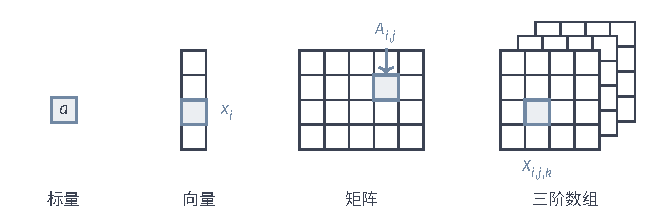
\includegraphics[width=112mm]{figures/00-shared/mathematical-preliminaries-upper/02-linear-spaces/tikz/comprehension-additions/scalar-vector-matrix-tensor.pdf}
  \caption{标量、向量、矩阵与三阶数组的区别。每个面板用蓝色标出一个数：标量本身就是这个数，向量用一个索引$i$定位，矩阵用行列两个索引$i,j$定位，三阶数组再加一个索引$k$选择切片。索引个数称为阶，各轴长度组成形状。}
  \label{fig:ls-scalar-vector-matrix-tensor}
\end{figure}

两个同形数组按位置逐项相加和数乘，规则与向量、矩阵相同。两个数组相加，仍要求形状相同、对应轴的含义相同。所以使用多维数组时，要先说清每条轴记录什么。同一个$b\times\ell\times d$数组，若把第二、三轴的含义弄反，后面的每一次汇总都会汇总到错误的轴上。

\subsection{张量的重排}
\label{sec:ls-tensor-operations}

有了记法，先看第一类运算：重排。轴置换与形状重整只改变元素记录在哪条轴、哪个位置上，既不改变数值，也不求和。下面先讨论这两种重排，再整理它们共同的性质。

\subsubsection{轴置换}
\label{sec:ls-tensor-reshaping}
\phantomsection
\label{sec:linear-algebra-tensors-structured-operations}

\term{维度重排}（permutation of axes）也称轴置换，它按给定顺序调换轴的位置，每个元素跟着自己的索引移动。计算时先写出新旧索引的对应，再按对应搬运元素。例如把$\bm X\in\mathbb R^{b\times\ell\times d}$的第二、三轴互换，得到$\bm Y\in\mathbb R^{b\times d\times\ell}$，
\[
 y_{i,k,j}=x_{i,j,k}.
\]
第一轴保持原位，每个样本的切片被转置：$\bm Y_{i,:,:}=(\bm X_{i,:,:})^\top$。下面取一个具体的小数组。
\begin{example}[交换后两条轴]
\label{ex:ls-axis-swap}
取$b=1$、$\ell=2$、$d=3$，这时数组只有一个样本切片
\[
 \bm X_{1,:,:}=\begin{bmatrix}1&2&3\\4&5&6\end{bmatrix}.
\]
按$y_{1,k,j}=x_{1,j,k}$逐个搬运元素。例如原来位于第$2$个位置、第$3$个特征的$6$，搬到$y_{1,3,2}$。全部搬完，得到
\[
 \bm Y_{1,:,:}=\begin{bmatrix}1&4\\2&5\\3&6\end{bmatrix}.
\]
新数组$\bm Y\in\mathbb R^{1\times3\times2}$的样本切片正是原切片的转置，数值一个也没有改变。
\end{example}
只有两条轴时，唯一不平凡的轴置换就是矩阵的转置。轴的含义跟着轴走，不因位置改变而改变：$\bm Y$的第二轴仍是特征，第三轴仍是位置。

\subsubsection{形状重整与向量化}

\term{形状重整}（reshape）分两步：先按指定的遍历顺序把全部元素读成一个数列，再把这个数列按同样的顺序装入另一种形状。它只要求元素总数不变。形状重整与转置都能把$2\times3$矩阵变成$3\times2$矩阵，但结果不同。
\begin{example}[按行重整与转置的区别]
\label{ex:ls-reshape-vs-transpose}
把
\[
 \bm A=\begin{bmatrix}1&2&3\\4&5&6\end{bmatrix}
\]
按行重整为$3\times2$数组：先按行读出数列$1,2,3,4,5,6$，再按行依次装入，得到下面的$\bm R$。作为对照，同时写出转置$\bm A^\top$：
\[
\begin{gathered}
\bm R=\begin{bmatrix}1&2\\3&4\\5&6\end{bmatrix},\\
\text{而}\qquad
 \bm A^\top=\begin{bmatrix}1&4\\2&5\\3&6\end{bmatrix}.
\end{gathered}
\]
$\bm R$与$\bm A^\top$形状相同、所含的数相同，排列却不同。$\bm A^\top$的第一列是$\bm A$原来的第一行$1,2,3$，$\bm R$的第一列却是$1,3,5$，把原来的行拆散了。
\end{example}
所以描述一次重整，除了目标形状，还要给出遍历顺序；形状对了，也不说明完成了轴交换。图~\ref{fig:vol1-add-linear-transpose-reshape}把两种结果并排放置。
\begin{figure}[!htb]
  \centering
  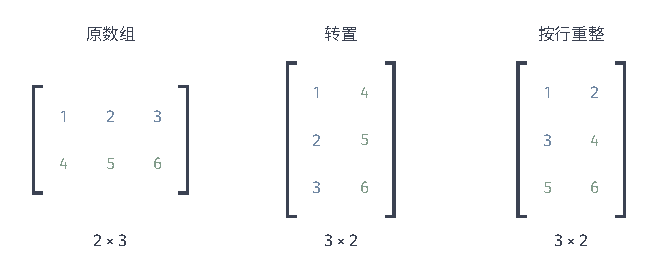
\includegraphics[width=112mm]{figures/00-shared/mathematical-preliminaries-upper/02-linear-spaces/tikz/comprehension-additions/linear-transpose-reshape.pdf}
  \caption{轴交换与按行重整。原数组两行为$(1,2,3)$与$(4,5,6)$；中图转置后两列分别保留原来的两行，右图则把按行读取的数列$1,2,3,4,5,6$依次装入$3\times2$数组。数字及其排列与正文示例相同。}
  \label{fig:vol1-add-linear-transpose-reshape}
\end{figure}

最常用的一种形状重整，是把矩阵按列堆叠成一个长列向量，称为\term{向量化}（vectorization）：
\[
 \operatorname{vec}(\bm A)=(a_{1,1},\ldots,a_{m,1},a_{1,2},\ldots,a_{m,2},\ldots,a_{1,n},\ldots,a_{m,n})^\top.
\]
$m\times n$矩阵的元素$a_{i,j}$位于第$i+(j-1)m$个位置。例如上面的$\bm A$给出$\operatorname{vec}(\bm A)=(1,4,2,5,3,6)^\top$，其中$a_{2,3}=6$位于第$2+(3-1)\cdot2=6$个位置。

多维数组也可以重整成矩阵，称为矩阵展开（unfolding）：把一部分轴合并成行索引，其余轴合并成列索引。例如把$\bm X\in\mathbb R^{b\times\ell\times d}$的前两轴合并为行，得到$b\ell\times d$矩阵，每行是一个样本在一个位置上的特征。合并哪些轴，决定了展开结果的形状，也决定了后续乘积汇总哪条轴。

\subsubsection{重排的性质}

固定轴的顺序和遍历规则以后，重排有三条性质：它不丢失信息，与逐项运算可交换，但一般的形状重整与矩阵乘法不相容。

\paragraph{可逆性}
目标形状与遍历顺序固定后，轴置换、形状重整与向量化都把一个数组一一对应到另一个数组，逆操作可以恢复原数组：
\[
 (\bm A^\top)^\top=\bm A,\qquad
 \operatorname{vec}^{-1}\bigl(\operatorname{vec}(\bm A)\bigr)=\bm A.
\]
这里$\operatorname{vec}^{-1}$把长度为$mn$的向量依次每$m$个一列装回$m\times n$矩阵。一般的轴置换按逆置换换回，形状重整按原顺序装回。所以重排保留全部信息。

\paragraph{线性}
\[
 \operatorname{vec}(a\bm A+b\bm B)=a\operatorname{vec}(\bm A)+b\operatorname{vec}(\bm B).
\]
轴置换与形状重整同样满足这一性质：它们只搬动元素，逐项的加法与数乘搬到新位置后不变。

\paragraph{与矩阵乘法的关系}
转置与乘法有整齐的规则
\[
 (\bm A\bm B)^\top=\bm B^\top\bm A^\top,
\]
一般的形状重整却没有。重整以后，每一行、每一列汇集的元素都变了，依赖行列结构的乘积、迹与行列式一般随之改变。下面的反例把示例~\ref{ex:ls-reshape-vs-transpose}中的$\bm R$误当作$\bm A^\top$使用。
\begin{example}[反例：重整不能代替转置]
\label{ex:ls-reshape-breaks-product}
仍取$\bm A$与按行重整得到的$\bm R$，
\[
 \bm A=\begin{bmatrix}1&2&3\\4&5&6\end{bmatrix},\qquad
 \bm R=\begin{bmatrix}1&2\\3&4\\5&6\end{bmatrix}.
\]
示例~\ref{ex:ls-gram-product-symmetric}已经算出
\[
 \bm A\bm A^\top=\begin{bmatrix}14&32\\32&77\end{bmatrix};
\]
而
\[
 \bm A\bm R=\begin{bmatrix}1+6+15&2+8+18\\4+15+30&8+20+36\end{bmatrix}=\begin{bmatrix}22&28\\49&64\end{bmatrix}.
\]
$\bm R$与$\bm A^\top$形状相同、所含的数相同，两个乘积却完全不同：$\bm A\bm R$不对称，迹也从$14+77=91$变成$22+64=86$。原因是乘积按行列配对元素，而重整改变了哪些元素同在一列。
\end{example}
把存储格式的改变误当成计算上的变换，是使用重整时最常见的错误。

\subsection{张量积}
\label{sec:ls-tensor-products}
\phantomsection
\label{sec:linear-algebra-joint-operations}

第二类运算把几个数组组合起来。最基本的情形是两个向量：把它们的全部两两乘积排成一个数组，就是张量积。

设$\bm x\in\mathbb R^m$、$\bm y\in\mathbb R^n$，\term{张量积}（tensor product）$\bm x\otimes\bm y$是$m\times n$数组，
\[
 (\bm x\otimes\bm y)_{i,j}=x_i y_j.
\]
写成矩阵，$\bm x\otimes\bm y=\bm x\bm y^\top$，正是分块乘法式~\eqref{eq:ls-product-outer-sum}中“一列乘一行”的矩阵。每个因子各占结果的一条轴，下面把这条轴称为该因子的槽位。三个向量的张量积$(\bm x\otimes\bm y\otimes\bm z)_{i,j,k}=x_i y_j z_k$有三个槽位，更多因子按同样规则逐槽位相乘。下面计算两个二维向量的张量积。
\begin{example}[两个二维向量的张量积]
\label{ex:ls-tensor-product-two-vectors}
取$\bm x=(1,2)^\top$与$\bm y=(3,-1)^\top$，把$x_i$与$y_j$的乘积填在位置$(i,j)$：
\[
 \bm x\otimes\bm y=\begin{pmatrix}1\cdot3&1\cdot(-1)\\2\cdot3&2\cdot(-1)\end{pmatrix}=\begin{pmatrix}3&-1\\6&-2\end{pmatrix}.
\]
第二行$(6,-2)$恰是第一行$(3,-1)$的$2$倍。一般地，第$i$行是$x_i\bm y^\top$，每一行都是$\bm y^\top$的倍数；同理，每一列都是$\bm x$的倍数。
\end{example}
两个因子的长度不必相同。图~\ref{fig:ls-tensor-product-slots}取$\bm u=(1,2)^\top$与三维的$\bm v=(3,-1,2)^\top$：第一个因子占行轴，第二个因子占列轴，结果的第$i$行是$u_i\bm v^\top$，第$j$列是$v_j\bm u$。
\begin{figure}[htbp]
  \centering
  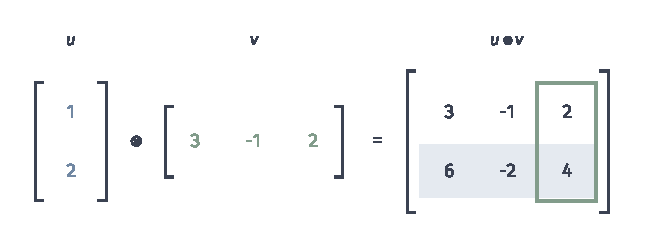
\includegraphics[width=112mm]{figures/00-shared/mathematical-preliminaries-upper/02-linear-spaces/matplotlib/ls-tensor-product-slots/ls-tensor-product-slots.pdf}
  \caption{张量积的两个槽位。左：$\bm u=(1,2)^\top\in\mathbb R^2$竖排，$\bm v=(3,-1,2)^\top\in\mathbb R^3$横排。右：$\bm u\otimes\bm v$是$2\times3$数组，行由$u_i$标记、列由$v_j$标记，位置$(i,j)$的元素为$u_iv_j$。蓝色实线框标出第2行$(6,-2,4)=u_2\bm v^\top$，绿色虚线框标出第3列$(2,4)^\top=v_3\bm u$。数值由定义直接相乘得到，是教学构造。}
  \label{fig:ls-tensor-product-slots}
\end{figure}

同样的配对规则适用于任意有限数组。设$\bm A$有$k$条轴、形状为$n_1\times\cdots\times n_k$，$\bm B$有$\ell$条轴、形状为$m_1\times\cdots\times m_\ell$。它们的数组张量积保留两组索引：
\[
 (\bm A\otimes\bm B)_{i_1,\ldots,i_k,j_1,\ldots,j_\ell}
 =a_{i_1,\ldots,i_k}b_{j_1,\ldots,j_\ell}.
\]
输出有$k+\ell$条轴，长度依次与输入的各轴相同；这里没有对任何索引求和。交换两个输入，会同时交换两组轴的次序。实数乘积$ab=ba$，并不意味着$\bm A\otimes\bm B$与$\bm B\otimes\bm A$相同。

形如$\bm x\otimes\bm y$的数组称为\term{简单张量}（simple tensor）。由示例~\ref{ex:ls-tensor-product-two-vectors}，简单张量的各行都是同一个向量的倍数。所以并非每个二阶数组都是简单张量，下面是一个反例。
\begin{example}[反例：单位矩阵不是简单张量]
\label{ex:ls-identity-not-simple}
$\bm I_2$的两行为$(1,0)$与$(0,1)$。假设$\bm I_2=\bm x\otimes\bm y$，则两行分别是$x_1\bm y^\top$与$x_2\bm y^\top$。两行都非零，所以$x_1,x_2\neq0$，两行都是$\bm y^\top$的非零倍数，从而彼此成比例。但$(1,0)$与$(0,1)$不成比例，矛盾。所以$\bm I_2$不能写成任何$\bm x\otimes\bm y$，它不是简单张量。
\end{example}
不过，每个$m\times n$数组$\bm T$都是简单张量的和：
\[
 \bm T=\sum_{i,j}t_{i,j}\,\bm e_i\otimes\bm f_j,
\]
其中$\bm e_i$、$\bm f_j$分别是$\mathbb R^m$与$\mathbb R^n$的标准坐标向量，$\bm e_i\otimes\bm f_j$只在位置$(i,j)$为$1$。

张量积的用处，是把同时依赖两组输入的计算，化为对单个数组的线性计算。设实值函数$B(\bm x,\bm y)$对$\bm x$、$\bm y$分别保持线性组合，这样的函数称为双线性的。把$\bm x=\sum_ix_i\bm e_i$、$\bm y=\sum_jy_j\bm f_j$代入，按两次线性展开，
\[
 B(\bm x,\bm y)=\sum_{i,j}x_iy_j\,B(\bm e_i,\bm f_j)=\sum_{i,j}g_{i,j}(\bm x\otimes\bm y)_{i,j}
 =\langle\bm G,\bm x\otimes\bm y\rangle_{\mathrm F},
\]
其中$g_{i,j}=B(\bm e_i,\bm f_j)$。所以双线性函数由一张固定的系数表$\bm G$决定，并且它作为$\bm x\otimes\bm y$的函数是线性的。以欧氏内积$B(\bm x,\bm y)=\bm x^\top\bm y$（$m=n$）为例，$g_{i,j}=\langle\bm e_i,\bm e_j\rangle$，即$\bm G=\bm I$，这时计算就是把$\bm x\otimes\bm y$的对角元加起来。

二阶张量与矩阵是同一组数的两种看法：张量强调每个槽位来自哪一组输入，矩阵强调行与列在乘法中的角色。

\subsubsection{张量积的性质}
\label{sec:ls-tensor-product-properties}

张量积的每个元素都是各因子元素的乘积，下面的性质都从这个元素公式逐槽位验证。

\paragraph{对每个因子线性}
\[
 \begin{gathered}
(a\bm x)\otimes\bm y=\bm x\otimes(a\bm y)=a(\bm x\otimes\bm y),\\
(\bm x+\bm x')\otimes\bm y=\bm x\otimes\bm y+\bm x'\otimes\bm y,\\
\bm x\otimes(\bm y+\bm y')=\bm x\otimes\bm y+\bm x\otimes\bm y'.
 \end{gathered}
\]
每个元素$x_iy_j$对$x_i$和$y_j$分别线性，逐项验证即得。

\paragraph{结合律}
\[
 (\bm x\otimes\bm y)\otimes\bm z=\bm x\otimes(\bm y\otimes\bm z),
\]
两边的$(i,j,k)$元素都是$x_iy_jz_k$。

\paragraph{交换槽位是转置}
\[
 \bm y\otimes\bm x=(\bm x\otimes\bm y)^\top,
\]
因为$\bm x\otimes\bm y$的$(i,j)$元素$x_iy_j$也是$\bm y\otimes\bm x$的$(j,i)$元素。所以一般$\bm x\otimes\bm y\neq\bm y\otimes\bm x$，两者相差一次轴置换。

\paragraph{Frobenius配对与范数分离}
\[
 \begin{gathered}
\langle\bm x\otimes\bm y,\bm x'\otimes\bm y'\rangle_{\mathrm F}
 =\langle\bm x,\bm x'\rangle\langle\bm y,\bm y'\rangle,\\
\lVert\bm x\otimes\bm y\rVert_{\mathrm F}=\lVert\bm x\rVert_2\,\lVert\bm y\rVert_2.
 \end{gathered}
\]
第一式来自$\sum_{i,j}x_iy_jx'_iy'_j=(\sum_ix_ix'_i)(\sum_jy_jy'_j)$；在第一式中取$\bm x'=\bm x$、$\bm y'=\bm y$，再开平方，得到第二式。下面在示例~\ref{ex:ls-tensor-product-two-vectors}的数组上核对第二式。
\begin{example}[张量积范数的数值核对]
\label{ex:ls-tensor-product-norm-check}
仍取$\bm x=(1,2)^\top$与$\bm y=(3,-1)^\top$，它们的张量积为
\[
 \bm x\otimes\bm y=\begin{pmatrix}3&-1\\6&-2\end{pmatrix}.
\]
按公式右端，只需两个向量各自的长度：$\lVert\bm x\rVert_2=\sqrt5$，$\lVert\bm y\rVert_2=\sqrt{10}$，乘积为$\sqrt5\cdot\sqrt{10}=\sqrt{50}=5\sqrt2$。直接对四个元素求Frobenius范数，
\[
 \lVert\bm x\otimes\bm y\rVert_{\mathrm F}=\sqrt{3^2+(-1)^2+6^2+(-2)^2}=\sqrt{50},
\]
两种算法一致。
\end{example}

\paragraph{与行列式的联系}
把张量积反对称化，得到$\bm x\otimes\bm y-\bm y\otimes\bm x$。它的$(i,j)$元素为
\[
 x_iy_j-x_jy_i=\det\begin{pmatrix}x_i&y_i\\x_j&y_j\end{pmatrix},
\]
即把$\bm x,\bm y$投影到第$i,j$两个坐标构成的平面后张成的有向面积（第~\ref{sec:ls-exterior-determinants}节）。交换$\bm x,\bm y$时，每个元素都变号。

\subsection{Kronecker积}

两个矩阵分别作用在两条轴上时，可以把联合作用写成一张大矩阵，这就是Kronecker积。对$\bm A\in\mathbb R^{m\times n}$、$\bm B\in\mathbb R^{p\times q}$，定义
\begin{equation}
 \bm A\otimes\bm B
 =\begin{bmatrix}
  A_{1,1}\bm B&\cdots&A_{1,n}\bm B\\
  \vdots&\ddots&\vdots\\
  A_{m,1}\bm B&\cdots&A_{m,n}\bm B
 \end{bmatrix}\in\mathbb R^{mp\times nq}.
 \label{eq:linear-algebra-kronecker-product}
\end{equation}
计算时，把$\bm A$的每个元素$A_{i,j}$替换成块$A_{i,j}\bm B$。下面计算一个二阶的例子。
\begin{example}[两个二阶矩阵的Kronecker积]
\label{ex:ls-kronecker-two-by-two}
取
\[
 \bm A=\begin{bmatrix}1&2\\3&4\end{bmatrix},\quad
 \bm B=\begin{bmatrix}0&1\\1&0\end{bmatrix},
\]
把$\bm A$的四个元素分别换成块$1\cdot\bm B$、$2\cdot\bm B$、$3\cdot\bm B$、$4\cdot\bm B$：
\[
 \bm A\otimes\bm B
 =\begin{bmatrix}
  1\cdot\bm B&2\cdot\bm B\\
  3\cdot\bm B&4\cdot\bm B
 \end{bmatrix}
 =\begin{bmatrix}0&1&0&2\\1&0&2&0\\0&3&0&4\\3&0&4&0\end{bmatrix}.
\]
结果是$4\times4$矩阵。每个$2\times2$块都是$\bm B$乘以$\bm A$的一个元素，块的排列照搬$\bm A$中元素的位置：$\bm A$的形状与元素决定块怎样排、各乘多少，$\bm B$决定每块内部的样子。
\end{example}
图~\ref{fig:ls-kronecker-block-structure}用另一组数展示这种逐元素替换得到的分块结构。
\begin{figure}[htbp]
  \centering
  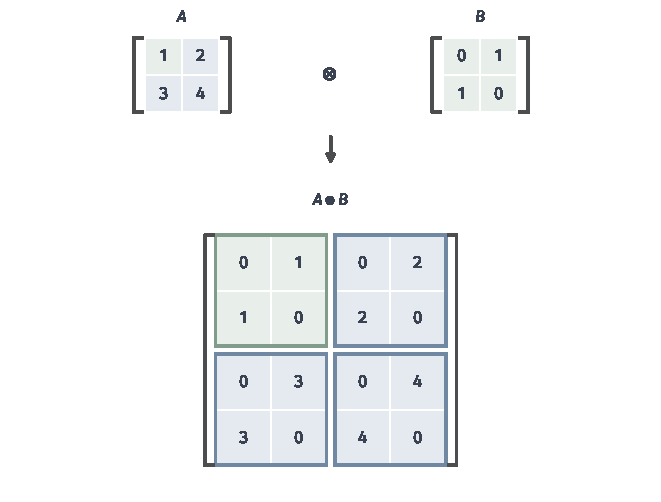
\includegraphics[width=112mm]{figures/00-shared/mathematical-preliminaries-upper/02-linear-spaces/matplotlib/ls-kronecker-block-structure/ls-kronecker-block-structure.pdf}
  \caption{Kronecker积的分块结构。上：$\bm A=\bigl(\begin{smallmatrix}1&2\\3&4\end{smallmatrix}\bigr)$、$\bm B=\bigl(\begin{smallmatrix}10&20\\30&40\end{smallmatrix}\bigr)$。下：$\bm A\otimes\bm B$是把$\bm A$的每个元素替换为该元素乘$\bm B$得到的$4\times4$分块矩阵，块边界用白线强调。数值由定义直接计算，是教学例。}
  \label{fig:ls-kronecker-block-structure}
\end{figure}

Kronecker积与张量积用同一个记号$\otimes$，两者记录的是同一组数，只是排法不同。两个列向量按式~\eqref{eq:linear-algebra-kronecker-product}相乘，得到$mn$维长向量$(x_1\bm y^\top,\ldots,x_m\bm y^\top)^\top$，它正是把$m\times n$数组$\bm x\otimes\bm y$按行读出的结果。例如$(1,2)^\top\otimes(3,-1)^\top=(3,-1,6,-2)^\top$，与示例~\ref{ex:ls-tensor-product-two-vectors}中的数组按行读出的结果相同。对一般矩阵，数组张量积保留四条轴，Kronecker积把它们排成两条轴。遇到记号$\otimes$时，须根据上下文和输出形状判断是哪一种。

\subsubsection{Kronecker积的性质}
\label{sec:ls-kronecker-products}

Kronecker积是分块矩阵，下面的乘法、转置、逆和迹的规则都可以用块运算验证。最后一条向量化恒等式在求解矩阵方程时要用到。

\paragraph{分别作用于两个槽位}
\[
 (\bm A\otimes\bm B)(\bm x\otimes\bm y)=(\bm A\bm x)\otimes(\bm B\bm y).
\]
按分块乘法，左侧第$i$块为$\sum_jA_{i,j}\bm B(x_j\bm y)=(\sum_jA_{i,j}x_j)\bm B\bm y=(\bm A\bm x)_i\,\bm B\bm y$，正是右侧的第$i$块。第一个槽位只经过$\bm A$，第二个槽位只经过$\bm B$，两个作用并排进行。矩阵乘法则不同，它把前后两次作用串成一条链。

\paragraph{混合乘积}
当$\bm A\bm C$与$\bm B\bm D$都有定义时，
\begin{equation}
 (\bm A\otimes\bm B)(\bm C\otimes\bm D)
 =(\bm A\bm C)\otimes(\bm B\bm D).
 \label{eq:matrix-analysis-kronecker-mixed-product}
\end{equation}
按分块乘法，左侧的块$(i,k)$为$\sum_j(A_{i,j}\bm B)(C_{j,k}\bm D)=(\sum_jA_{i,j}C_{j,k})\bm B\bm D=(\bm A\bm C)_{i,k}\bm B\bm D$，恰是右侧的块。上一条是$\bm C,\bm D$各只有一列的特例。

\paragraph{转置}
\[
 (\bm A\otimes\bm B)^\top=\bm A^\top\otimes\bm B^\top.
\]
分块矩阵转置时，块的位置交换，每块各自转置，所以第$(j,i)$块为$A_{i,j}\bm B^\top$，正是$\bm A^\top\otimes\bm B^\top$的第$(j,i)$块。

\paragraph{逆}
\[
 (\bm A\otimes\bm B)^{-1}=\bm A^{-1}\otimes\bm B^{-1}\qquad(\bm A,\bm B\text{都可逆}).
\]
由混合乘积，$(\bm A\otimes\bm B)(\bm A^{-1}\otimes\bm B^{-1})=(\bm A\bm A^{-1})\otimes(\bm B\bm B^{-1})=\bm I\otimes\bm I=\bm I$，另一侧同理。

\paragraph{迹}
\[
 \operatorname{tr}(\bm A\otimes\bm B)=\operatorname{tr}\bm A\,\operatorname{tr}\bm B\qquad(\bm A,\bm B\text{都是方阵}).
\]
只有对角块$A_{i,i}\bm B$的对角元落在主对角线上，所以迹为$\sum_iA_{i,i}\operatorname{tr}\bm B=\operatorname{tr}\bm A\,\operatorname{tr}\bm B$。

\paragraph{向量化恒等式}
对$\bm A\in\mathbb R^{p\times m}$、$\bm X\in\mathbb R^{m\times n}$、$\bm B\in\mathbb R^{n\times q}$，
\begin{equation}
 \operatorname{vec}(\bm A\bm X\bm B)
 =(\bm B^\top\otimes\bm A)\operatorname{vec}(\bm X).
 \label{eq:matrix-analysis-vec-kronecker}
\end{equation}
比较两侧输出的第$j$段（长度为$p$）。左侧是$\bm A\bm X\bm B$的第$j$列，$\bm A\bm X\bm B_{:,j}=\sum_kB_{k,j}\bm A\bm X_{:,k}$。右侧矩阵的第$j$个块行为$(B_{1,j}\bm A,\ldots,B_{n,j}\bm A)$，与$\operatorname{vec}(\bm X)$的各段$\bm X_{:,1},\ldots,\bm X_{:,n}$相乘，也得到$\sum_kB_{k,j}\bm A\bm X_{:,k}$。逐元素写出，两侧$(i,j)$位置的元素都是$\sum_{\ell=1}^m\sum_{k=1}^n A_{i,\ell}X_{\ell,k}B_{k,j}$。

固定$\bm A,\bm B$后，这个恒等式把“两侧同时乘矩阵”写成长向量$\operatorname{vec}(\bm X)$左乘一张矩阵。关于未知矩阵的方程由此化成普通的线性方程组；第~\ref{chap:matrix-equations}章求解矩阵方程时会用到它。

\subsection{指标缩约}
\label{sec:ls-tensor-operation-properties}
\label{sec:ls-tensor-contraction}

张量积保留全部槽位；第三类运算缩约则相反，它沿指定的轴求和，减少轴的个数。

计算时选定一对或几对长度相同的轴，让每对轴共用同一个求和索引，逐项相乘后对这些索引求和。被求和的轴消失，其余的轴按原次序保留，组成输出的形状。写出索引，就能检查哪些轴被消去、哪些轴被保留。下面用两个例子说明。
\begin{example}[两种缩约的输出形状]
\label{ex:ls-contraction-shapes}
（1）设$\bm A\in\mathbb R^{m\times d\times r}$，$\bm B\in\mathbb R^{d\times n\times r}$。让$\bm A$的第二轴与$\bm B$的第一轴共用索引$k$，两者的第三轴共用索引$s$：
\[
 c_{i,j}=\sum_{k=1}^d\sum_{s=1}^r a_{i,k,s}b_{k,j,s}.
\]
两对轴同时被消去，只剩$\bm A$的第一轴$i$和$\bm B$的第二轴$j$，所以输出是$m\times n$矩阵。

（2）设$\bm X\in\mathbb R^{b\times\ell\times d}$记录一批样本在各位置上的特征，$\bm W\in\mathbb R^{d\times h}$。让$\bm X$的最后一轴与$\bm W$的第一轴共用索引$k$：
\[
 z_{i,j,t}=\sum_{k=1}^d x_{i,j,k}w_{k,t}.
\]
这次只消去$k$，保留$i,j,t$，输出形状为$b\times\ell\times h$。与（1）相比，这里只配对一对轴，样本轴和位置轴都原样保留：每个样本、每个位置上的$d$维特征都乘了同一个矩阵$\bm W$。
\end{example}
图~\ref{fig:ls-tensor-contraction}画出沿一对轴求和、保留其余轴的过程。
\begin{figure}[htbp]
  \centering
  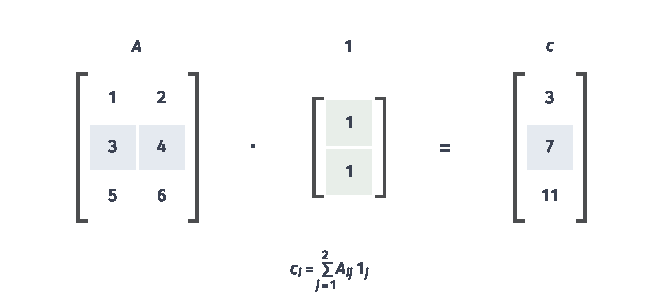
\includegraphics[width=112mm]{figures/00-shared/mathematical-preliminaries-upper/02-linear-spaces/matplotlib/ls-tensor-contraction/ls-tensor-contraction.pdf}
  \caption{张量缩约沿选中的一对轴求和、保留其余轴。左：二阶张量按行和列着色；选中列轴（虚线箭头）沿列求和，输出对每行汇总为一个值。右：缩约后得到$3$个输出，分别对应原矩阵三行的行和，颜色由红（小）经黄到蓝（大）。张量与数值均为解析教学例。}
  \label{fig:ls-tensor-contraction}
\end{figure}

图中对每行求和，也可以看成与全$1$向量沿列轴缩约。前两节的几种运算都是缩约：
\begin{itemize}
 \item 内积$\sum_jx_jy_j$缩约两个向量唯一的一对轴，输出标量；
 \item 矩阵乘法$\sum_\ell a_{i,\ell}b_{\ell,j}$只消去左因子的列轴与右因子的行轴这一对；
 \item 迹$\sum_iA_{i,i}$让同一个矩阵的行轴与列轴共用一个索引，再求和；
 \item Frobenius内积$\sum_{i,j}a_{i,j}b_{i,j}$同时缩约两对轴。
\end{itemize}

\subsubsection{缩约的性质}

缩约只由有限次乘法与求和组成，因此满足以下规则。

\paragraph{线性}
固定参与配对的另一个数组，缩约对被作用的数组是线性的。以示例~\ref{ex:ls-contraction-shapes}（2）中与$\bm W$的缩约为例，把$\bm X$换成$a\bm X+b\bm X'$，
\[
 \sum_{k=1}^d\bigl(a\,x_{i,j,k}+b\,x'_{i,j,k}\bigr)w_{k,t}
 =a\sum_{k=1}^d x_{i,j,k}w_{k,t}+b\sum_{k=1}^d x'_{i,j,k}w_{k,t},
\]
输出变为两个输出的$a$倍与$b$倍之和。一般情形同理：每个输出元素都是被作用数组元素以固定系数作的加权和。

\paragraph{求和次序可交换}
多对轴的缩约是有限和，结果与先消去哪一对轴无关。例如示例~\ref{ex:ls-contraction-shapes}中的$c_{i,j}$，可以先对$s$求和得到中间数组，再对$k$求和，也可以反过来：
\[
 c_{i,j}=\sum_{k=1}^d\Bigl(\sum_{s=1}^r a_{i,k,s}b_{k,j,s}\Bigr)
 =\sum_{s=1}^r\Bigl(\sum_{k=1}^d a_{i,k,s}b_{k,j,s}\Bigr).
\]

\paragraph{简单张量系数可分离}
设一次计算同时依赖三组向量$\bm x\in\mathbb R^m$、$\bm y\in\mathbb R^n$、$\bm z\in\mathbb R^p$。若系数数组是简单张量$\bm a\otimes\bm b\otimes\bm c$，则
\begin{equation}
 \left\langle\bm a\otimes\bm b\otimes\bm c,
 \bm x\otimes\bm y\otimes\bm z\right\rangle_{\mathrm F}
 =(\bm a^\top\bm x)(\bm b^\top\bm y)(\bm c^\top\bm z).
 \label{eq:linear-algebra-rank-one-contraction}
\end{equation}
这是因为$\sum_{i,j,k}a_ib_jc_kx_iy_jz_k=(\sum_ia_ix_i)(\sum_jb_jy_j)(\sum_kc_kz_k)$：三重求和分离成三个内积的乘积，计算量从$mnp$项降到$m+n+p$项。下面用一组小数值核对。
\begin{example}[简单张量系数的分离计算]
\label{ex:ls-rank-one-contraction-check}
取$m=n=p=2$，系数向量为$\bm a=(1,2)^\top$、$\bm b=(3,-1)^\top$、$\bm c=(2,1)^\top$，输入为$\bm x=(2,1)^\top$、$\bm y=(1,1)^\top$、$\bm z=(1,-1)^\top$。按式~\eqref{eq:linear-algebra-rank-one-contraction}右端，只需三个内积：
\[
 \begin{gathered}
 \bm a^\top\bm x=1\cdot2+2\cdot1=4,\qquad
 \bm b^\top\bm y=3\cdot1+(-1)\cdot1=2,\\
 \bm c^\top\bm z=2\cdot1+1\cdot(-1)=1.
 \end{gathered}
\]
三个内积相乘得$4\cdot2\cdot1=8$。若直接展开三重求和，要累加$2^3=8$项、每项是六个数的乘积，结果同样是$8$。分离计算只需对$m+n+p=6$个坐标各做一次乘法，维数增大时，它比逐项展开省下的计算迅速增多。
\end{example}

\paragraph{非线性操作不是缩约}
由上面的线性，固定配对数组的缩约$\mathcal C$满足$\mathcal C(2\bm X)=2\,\mathcal C(\bm X)$。逐元素平方这样的逐元素非线性操作不满足这一点：只要$x_{i,j}\neq0$，
\[
 (2x_{i,j})^2=4x_{i,j}^2\neq2x_{i,j}^2,
\]
所以它不是缩约；$\operatorname{softmax}$等操作同样不是缩约。一个模型若由缩约与这些操作交替组成，那么即使固定了系数、每一步缩约都是线性的，也不能由此推出整个模型是线性的。

\section{本章小结}
\label{sec:ls-operations-summary}

本章按定位一个数所需的索引个数，依次讨论了向量、矩阵与张量的运算。对每种运算，我们都交代了输入条件、输出形状和可用的规则。

向量的加法与数乘逐坐标进行，组合起来就是线性组合。欧氏内积把两个同维向量配成一个数，长度和$p$范数用一个非负数衡量向量的大小。$p$范数非负、正定、齐次，并满足三角不等式，后者由Hölder不等式与Minkowski不等式证明。范数与内积的一般理论分别在第~\ref{chap:normed-spaces}章与第~\ref{chap:inner-product-spaces}章建立。

矩阵乘法来自两次加权求和的复合。它满足结合律与分配律，但不满足交换律与消去律。初等行变换都可以撤销，每一种都等于左乘一个可逆的初等矩阵。

逆矩阵撤销一次乘法：对角矩阵与二阶方阵有直接的求逆公式，一般方阵的求逆归结为解$n$个系数矩阵相同的方程，具体算法留到第~\ref{sec:ls-gaussian-elimination}节。矩阵的幂记录同一矩阵的反复作用。

行列式、迹和Frobenius内积把矩阵变成一个数。行列式是方阵对有向体积的缩放倍数，它非零恰好对应方阵可逆；由古典伴随还可以证明，方阵只要有一侧的逆，这个单侧逆就是逆矩阵。迹只累加对角元素，满足循环性。Frobenius内积配对两个同形矩阵的全部元素，由它得到Frobenius范数。

张量把索引推广到任意多个。重排只改变元素的位置，张量积与Kronecker积保留各因子的全部轴，缩约沿指定的轴求和；内积、矩阵乘法与迹都是缩约的特例。

本章出现了好几种“乘积”，它们的区别在于对索引做什么：有的配对后求和，有的在同一位置相乘而不求和，有的把两组索引全部保留。表~\ref{tab:linear-algebra-products-and-shapes}按这一区别汇总它们的形状条件与输出。遇到一个乘积记号时，先看它消去哪些索引、保留哪些索引，再判断输出的形状与含义。

\begin{table*}[htbp]
 \centering\small
 \begin{tabularx}{\linewidth}{@{}lXX@{}}
  \toprule
  运算 & 形状条件与输出 & 索引作用\\
  \midrule
  $\langle\bm x,\bm y\rangle$ & 两个$n$维向量，输出标量 & 配对后汇总\\
  $\bm A\bm B$ & $(m\times n)(n\times p)\to m\times p$ & 汇总共同索引\\
  $\bm A\odot\bm B$ & 同为$m\times n$，输出仍为$m\times n$ & 同位置相乘，不求和\\
  $\bm x\otimes\bm y$ & $m$维与$n$维向量$\to m\times n$ & 保留两条轴，不求和\\
  $\bm A\otimes\bm B$ & $(m\times n)$与$(p\times q)\to(mp)\times(nq)$ & 保留两组成对索引\\
  缩约 & 被缩约的各对轴长度相同 & 消去指定轴，保留其余轴\\
  \bottomrule
 \end{tabularx}
 \caption{本章各种乘积的形状。同一类乘积记号可能对应不同操作：先看消去哪些索引，再判断输出的形状和含义。}
 \label{tab:linear-algebra-products-and-shapes}
\end{table*}

本章只把这些数组当作具体的数表。第~\ref{chap:linear-representation}章讨论它们记录的是什么：同一个对象换一组方向后坐标怎样改变，矩阵怎样记录线性映射。一般空间中的大小在第~\ref{chap:normed-spaces}章讨论，夹角与正交在第~\ref{chap:inner-product-spaces}章讨论。矩阵乘法的结合律、逆矩阵和幂在后文反复出现：矩阵反复作用的长期行为在第~\ref{chap:linear-recurrence-stability}章讨论，误差经过一次矩阵作用被放大多少在第~\ref{chap:condition-and-spectral-perturbation}章讨论，方程的解与求解方法从第~\ref{chap:linear-solution-selection}章开始讨论。


\chapter{线性空间、映射与坐标}
\label{chap:linear-representation}
\label{chap:linear-algebra-and-matrix-analysis}
\label{chap:linear-algebra}

第~\ref{chap:linear-operations}章把数据记成数组，并规定了数组的运算，但没有区分数组本身和它记录的对象。以仿射函数$f_{a,b}(t)=a+bt$为例。它是一个函数，两个仿射函数相加或缩放后仍是仿射函数。选定$1$与$t$这两个基本函数以后，$f_{a,b}$才记成一列数$(a,b)^{\top}$；换一组基本函数，这列数随之改变，函数本身却不变。

矩阵同样有两重身份。设计矩阵$\bm X_\varepsilon$（式~\eqref{eq:linear-algebra-nearly-collinear-design}）是一张$3\times2$的数表，它还记录了一个作用：把两个系数送到三个拟合值。要在不同的记录之间换算，又不被记录方式误导，就要把对象和记录对象的数分开。

本章按这一区分展开。记录之前，先要说清对象在什么范围内作线性组合：第~\ref{sec:ls-vector-spaces}节把数组、函数等能相加和缩放的对象统一为线性空间，并研究其中对线性组合封闭的子空间，以及“有意忽略一个子空间中的差别”得到的商空间。第~\ref{sec:ls-bases-dimension-coordinates}节在空间中选定一组基，用张成与线性无关保证每个对象有唯一的一组系数，即坐标；基的个数给出维数，换基时坐标按可逆矩阵换算，对象本身不变。

对象记录清楚以后，再记录对象之间保持线性组合的作用。第~\ref{sec:ls-linear-maps}节说明，选定两端的基，线性映射就记成矩阵；核与像分别描述映射消去的输入和能到达的输出；换基改变矩阵而不改变映射，由此得到相抵与相似两种关系。把向量线性地读成一个数的规则，即线性泛函，留到第~\ref{chap:dual-spaces}章。

本章在实数域上展开，涉及复数时另作说明。全章只用加法和数乘，所需的矩阵运算都来自第~\ref{chap:linear-operations}章；长度与收敛由第~\ref{chap:normed-spaces}章引入，夹角与正交由第~\ref{chap:inner-product-spaces}章引入。

% 第2章第1节：线性空间与子空间（向量空间；子空间及其包含、交、和、直和与商空间）。

\section{线性空间与子空间}
\label{sec:ls-vector-spaces}
\label{sec:linear-algebra-vector-spaces-coordinates}

第~\ref{chap:linear-operations}章的数组和本章开头的仿射函数都能相加和缩放。用一组方向记录这些对象之前，要先说清线性组合在什么范围内进行。本节先给出线性空间的定义，再讨论空间内部对线性组合封闭的部分，即子空间，以及子空间之间的比较、合并和商空间。

\subsection{线性空间的定义与示例}
\label{sec:ls-space-axioms}

第~\ref{sec:ls-vector-operation-rules}节验证过，同形数组的加法与数乘满足八条运算规则。其他对象也满足同样的规则：平面上的位移可以首尾相接，有限信号可以按幅度放大，多项式可以逐点相加。后面关于分解、方程的解和维数的结论只用到这八条规则，与对象具体是数组、位移、信号还是多项式无关。

因此，把带有这样的加法与数乘的集合统称为线性空间，其中的元素统称为向量。从此，“向量”指可以作线性组合的对象，不再要求它是一列数。

\begin{definition}[实线性空间]
\label{def:ls-real-vector-space}
设$V$是一个集合，给定加法（任意$\bm u,\bm v\in V$对应$\bm u+\bm v\in V$）与实数数乘（任意$a\in\mathbb R$、$\bm u\in V$对应$a\bm u\in V$）。若对任意$\bm u,\bm v,\bm w\in V$和$a,b\in\mathbb R$，下面八条规则成立，就称$V$为\term{向量空间}（也称线性空间，vector space）：
\begin{enumerate}
 \item 加法交换律：$\bm u+\bm v=\bm v+\bm u$。
 \item 加法结合律：$(\bm u+\bm v)+\bm w=\bm u+(\bm v+\bm w)$。
 \item 零元：存在$\bm0\in V$，使$\bm u+\bm0=\bm u$对每个$\bm u$成立。
 \item 加法逆元：每个$\bm u$都有$-\bm u\in V$，使$\bm u+(-\bm u)=\bm0$。
 \item 数乘结合律：$a(b\bm u)=(ab)\bm u$。
 \item 数乘对数的分配律：$(a+b)\bm u=a\bm u+b\bm u$。
 \item 数乘对向量的分配律：$a(\bm u+\bm v)=a\bm u+a\bm v$。
 \item 单位数乘：$1\bm u=\bm u$。
\end{enumerate}
\end{definition}
定义包含两层要求。第一层是\emph{封闭}：加法和数乘的结果必须留在$V$中，否则运算无法在$V$内进行。第二层是\emph{规则}：前四条说加法像数的加法一样可以交换、结合，有零元和相反元；后四条说数乘与加法按熟悉的方式配合。

有了这些规则，有限次线性运算无论怎样加括号、怎样展开，结果都相同。所以对任意$\bm v_1,\ldots,\bm v_k\in V$与实数$a_1,\ldots,a_k$，加权和$\sum_{j=1}^ka_j\bm v_j$有确定的意义。它仍称为这组向量的线性组合，与第~\ref{sec:ls-vector-operations}节对数组的定义一致。

标量也可以取复数。复线性空间满足同样的八条规则，只是数乘允许任意复数。

允许哪些标量会改变线性结构。$\mathbb C$作为复线性空间时，每个元素都是$1$的复数倍；只允许实数数乘时，表示$a+b\mathrm i$需要$1$与$\mathrm i$两个方向。复数域上的基与线性映射按同样的方式定义，内积则要处理共轭。本章其余推导在实数域中进行。

常见的具体空间都满足定义。$\mathbb R^d$与全体$m\times d$实矩阵在逐项运算下是线性空间，第~\ref{sec:ls-vector-operation-rules}节已逐条验证。次数不超过$k$的实多项式组成的集合
\[
 P_k=\{a_0+a_1t+\cdots+a_kt^k:a_0,\ldots,a_k\in\mathbb R\}
\]
在逐点相加与数乘下也是线性空间：两个这样的多项式相加或乘以实数，次数仍不超过$k$；八条规则则逐点继承实数运算的规则。本章开头的仿射函数全体正是$P_1$。

并非每个由向量组成的集合都是线性空间。下面两个$\mathbb R^d$的子集沿用$\mathbb R^d$的运算，分别破坏了加法封闭与数乘封闭。
\begin{example}[反例：仿射约束集与非负向量集]
\label{ex:ls-non-vector-space-sets}
考虑第一坐标固定为$1$的向量与各坐标都非负的向量：
\[
 \begin{gathered}
S_1=\{\bm x\in\mathbb R^d:x_1=1\}\\
S_2=\{\bm x\in\mathbb R^d:x_j\geq0,\ j=1,\ldots,d\},
 \end{gathered}
\]
两者都沿用$\mathbb R^d$的逐项加法与数乘。

$S_1$的问题出在加法上。任取$\bm x,\bm y\in S_1$，和的第一坐标是
\[
 x_1+y_1=2\neq1,
\]
所以$\bm x+\bm y$已经离开$S_1$；同样，零向量的第一坐标为$0$，$S_1$连零向量都不含。

$S_2$则相反：两个非负向量相加仍然非负，加法没有问题，但数乘允许负数。$\bm e_1$属于$S_2$，乘以$-1$后第一坐标变成$-1$，就不在$S_2$中了。

所以$S_1$对加法不封闭，$S_2$对数乘不封闭，二者都不是线性空间。两种失败分别对应定义中两种运算的封闭要求。
\end{example}
可见，判断一个集合是不是线性空间，要逐项检查运算是否封闭、规则是否成立，不能只看集合的形状。

\subsection{子空间、和与直和}
\label{sec:ls-subspaces}
\label{sec:linear-algebra-relations}
\label{sec:linear-algebra-subspace-relations}
\label{sec:ls-subspace-definition}

线性空间中常有一部分元素自己构成线性空间，例如平面中过原点的直线、齐次方程组的全部解。后面要处理的许多对象都是这样的部分：一组方向能到达的对象、一个映射消去的输入、方程的解，一般都只占空间的一部分。下面先给出判定条件，再比较和合并这些部分。

\paragraph{子空间的判定}
设$U$是$V$的非空子集。若$U$对线性组合封闭，即对任意$\bm u,\bm v\in U$和$a,b\in\mathbb R$都有$a\bm u+b\bm v\in U$，就称$U$为$V$的\term{线性子空间}（linear subspace），简称子空间。

这一条件已足以保证$U$在$V$的运算下构成线性空间。取$a=b=1$得加法封闭，取$b=0$得数乘封闭；取$a=b=0$得$\bm0\in U$，取$a=-1$、$b=0$得$-\bm u\in U$。其余规则对$V$的全部元素成立，自然也对$U$的元素成立。所以判断子空间只需检查这一条封闭条件，不必逐条核对八条规则。

每个空间都有两个平凡子空间：只含零向量的$\{\bm0\}$和$V$本身。下面用判定条件检查三个常见集合。
\begin{example}[过原点的直线、平移的直线与齐次解集]
\label{ex:ls-subspace-checks}
取平面中的非零向量$\bm u$、不在直线$\{c\bm u:c\in\mathbb R\}$上的点$\bm p$，以及矩阵$\bm A\in\mathbb R^{m\times d}$，考察下面三个集合：
\[
 \begin{gathered}
 L_0=\{c\bm u:c\in\mathbb R\},
 \qquad
 L_1=\{\bm p+c\bm u:c\in\mathbb R\},\\
 N=\{\bm x\in\mathbb R^d:\bm A\bm x=\bm0\}.
 \end{gathered}
\]

对$L_0$和$N$，只需检查线性组合是否留在集合内。$L_0$中任意两个元素$c_1\bm u$与$c_2\bm u$的组合是
\[
 a(c_1\bm u)+b(c_2\bm u)=(ac_1+bc_2)\bm u,
\]
仍是$\bm u$的倍数。

$N$中任取两个解$\bm x,\bm y$，由式~\eqref{eq:prelim-matrix-linearity}，
\[
 \bm A(a\bm x+b\bm y)=a\bm A\bm x+b\bm A\bm y=\bm0,
\]
所以组合$a\bm x+b\bm y$仍是解。两者都是子空间。

$L_1$在第一步就不满足要求：子空间必含零向量，而$L_1$不含。若$\bm p+c\bm u=\bm0$，则$\bm p=-c\bm u$落在$L_0$上，与$\bm p$的取法矛盾。因此同一个方向$\bm u$给出的直线，过原点时是子空间，平移离开原点后就不是了。
\end{example}
$L_1$由子空间$L_0$沿$\bm p$平移得到。示例~\ref{ex:ls-non-vector-space-sets}中的约束集$S_1=\{\bm x:x_1=1\}$也是如此：它由齐次解集$\{\bm x:x_1=0\}$沿$\bm e_1$平移得到，是一个仿射集合，同样不是子空间。

同一个空间$V$中的几个子空间可以从四个方面比较：一个是否含于另一个，二者有哪些公共向量，合起来能到达哪里，合并后的分解是否唯一。这四个方面分别由包含、交、和与直和描述。它们只涉及线性组合，不涉及长度或夹角。

\paragraph{包含}
\phantomsection
\label{sec:ls-subspace-inclusion}
若子空间$U$的每个元素都属于子空间$W$，就记$U\subseteq W$。这时$U$在$W$中对线性组合封闭，因而也是$W$的子空间。包含只比较两个集合的范围；两个子空间的“大小”要等下一节定义了维数才能比较。

\paragraph{交}
\phantomsection
\label{sec:ls-intersection}
两个子空间$U,W\subseteq V$的交$U\cap W$由同时属于二者的元素组成。它仍是子空间：若$\bm x,\bm y\in U\cap W$，则二者同在$U$中，也同在$W$中，所以$a\bm x+b\bm y$同属两边。

任何同时含于$U$与$W$的子空间，其元素都属于交，所以交是同时含于二者的最大子空间。

在平面中，两条重合的过原点直线的交是整条直线，两条不同的过原点直线的交只有零向量。交为零只说明两个子空间没有公共的非零向量，不说明二者合起来能到达整个空间。例如$\mathbb R^3$中两条不同的过原点直线交为零，合起来只能到达一个平面。

当$U,W$分别由齐次线性方程组描述时，交就是同时满足两组方程的解集合。例如$U=\{\bm x:x_1=0\}$与$W=\{\bm x:x_2=0\}$的交是$\{\bm x:x_1=x_2=0\}$。求交因此化为解联立的齐次方程组，可以用第~\ref{sec:ls-gaussian-elimination}节的消元求出；解集的系统讨论见第~\ref{chap:linear-solution-selection}章。

\paragraph{和}
\phantomsection
\label{sec:ls-sum}
把两个子空间中的向量相加，能得到的全部向量组成和空间
\[
 U+W=\{\bm u+\bm w:\bm u\in U,\ \bm w\in W\}.
\]
它对线性组合封闭：
\[
 a(\bm u_1+\bm w_1)+b(\bm u_2+\bm w_2)=(a\bm u_1+b\bm u_2)+(a\bm w_1+b\bm w_2),
\]
右端两个括号分别属于$U$与$W$。任何同时包含$U$与$W$的子空间都必须含有每个$\bm u+\bm w$，所以$U+W$是同时包含二者的最小子空间。

同时包含$U$与$W$的最小集合是并集$U\cup W$，但并集一般对加法不封闭，不能代替和空间。
\begin{example}[反例：两条坐标轴的并]
\label{ex:ls-union-not-subspace}
平面上的两条坐标轴$U=\{(s,0)^\top:s\in\mathbb R\}$与$W=\{(0,s)^\top:s\in\mathbb R\}$都是子空间。它们的并$U\cup W$含有$\bm e_1$与$\bm e_2$，却不含二者之和：$\bm e_1+\bm e_2=(1,1)^\top$的两个坐标都不为零，既不在$U$中，也不在$W$中。

所以$U\cup W$对加法不封闭，不是子空间。要得到子空间，必须补入所有形如$(s,0)^\top+(0,t)^\top$的向量，结果是整个平面，即$U+W=\mathbb R^2$。
\end{example}
和空间就是在并集之外补入了$\bm u+\bm w$这类必需的线性组合。

\paragraph{直和与补空间}
\phantomsection
\label{sec:ls-direct-sum}
和空间中的向量都能写成$\bm u+\bm w$，但写法未必唯一。在平面上取两条不平行的过原点直线，每个向量都能拆成分别落在两条直线上的两部分，而且拆法唯一。唯一与否由两个子空间的交决定。
\begin{theorem}[和的分解唯一的条件]
\label{thm:ls-direct-sum-uniqueness}
设$U,W$是$V$的子空间。$U+W$中每个向量写成$\bm u+\bm w$（$\bm u\in U$，$\bm w\in W$）的方式都唯一，当且仅当
\[
 U\cap W=\{\bm0\}.
\]
\end{theorem}
\begin{proof}
充分性：若$\bm u_1+\bm w_1=\bm u_2+\bm w_2$，移项得
\[
 \bm u_1-\bm u_2=\bm w_2-\bm w_1 .
\]
左边在$U$中，右边在$W$中，所以这个向量属于$U\cap W$，只能是零。于是$\bm u_1=\bm u_2$，$\bm w_1=\bm w_2$。

必要性：若交中有非零向量$\bm z$，则$\bm z\in U$、$-\bm z\in W$，等式
\[
 \bm0=\bm0+\bm0=\bm z+(-\bm z)
\]
给出零向量的两种不同分解，唯一性不成立。
\end{proof}

满足$U\cap W=\{\bm0\}$时，称和$U+W$为\term{直和}（direct sum），记为$U\oplus W$。唯一分解不要求两个子空间互相垂直：平面中任意两条不平行的过原点直线都构成直和。

若还有$U+W=V$，就写$V=U\oplus W$，并称$W$为$U$在$V$中的\term{补空间}（complement）。补空间一般不唯一：平面中一条过原点的直线，以任何不平行于它的过原点直线为补空间。

补空间总是存在，证明要用到下一节的基扩充（第~\ref{sec:ls-dimension}节）。

\subsection{商空间}
\phantomsection
\label{sec:ls-quotient-spaces}
\label{sec:linear-algebra-equivalence-relations}
和与直和把子空间合并起来。有时需要反过来，有意忽略某个子空间内的差别。

例如只关心仿射函数$f_{a,b}(t)=a+bt$在$t=0$处的值，即截距$a$时，$f_{a,b}$与$f_{a,b'}$没有区别；二者之差$(b-b')t$落在子空间$\{st:s\in\mathbb R\}$中。

非齐次约束$x_1=1$的解也有同样的结构。它的解集合$\{\bm e_1+\bm n:n_1=0\}$由一个特解加上齐次解子空间$\{\bm n:n_1=0\}$中的全部向量组成，任意两个解之差都落在这个子空间里。两个例子的共同点是：相差某个子空间中的向量，就视为相同。

把这一点写成关系。设$U$是$V$的子空间，规定$\bm x\sim\bm y$当且仅当$\bm x-\bm y\in U$。它是一个等价关系，即同时满足自反、对称与传递三条性质的关系。三条性质逐一验证如下：
\begin{enumerate}
\item 由$\bm x-\bm x=\bm0\in U$得自反性；
\item 由$\bm x-\bm y\in U$蕴含$\bm y-\bm x\in U$得对称性；
\item 由$(\bm x-\bm y)+(\bm y-\bm z)=\bm x-\bm z\in U$得传递性。
\end{enumerate}

$\bm x$所在的等价类为
\[
 \bm x+U=\{\bm x+\bm n:\bm n\in U\},
\]
即子空间$U$沿$\bm x$平移所得的集合。

两个类相等，不要求代表元相等，只要求代表元之差落在$U$中。

全部等价类把$V$分成互不重叠的块。图~\ref{fig:ls-quotient-equivalence-classes}在平面上画出这种划分：$U$是$x$轴，每条平行于$x$轴的直线是一个等价类。
\begin{figure}[htbp]
  \centering
  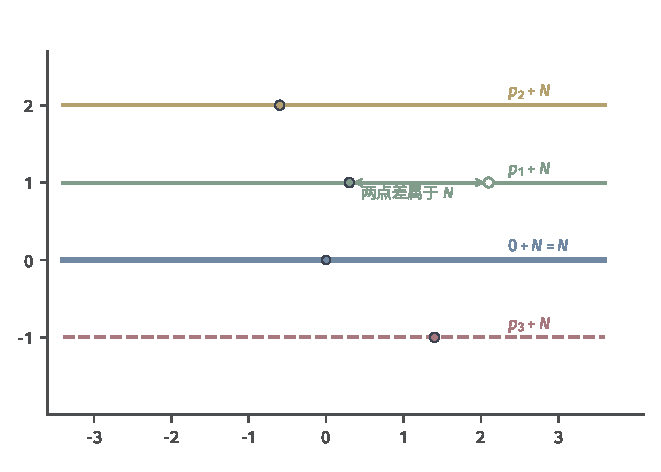
\includegraphics[width=112mm]{figures/00-shared/mathematical-preliminaries-upper/02-linear-spaces/matplotlib/ls-quotient-equivalence-classes/ls-quotient-equivalence-classes.pdf}
  \caption{商空间的等价类。$V=\mathbb R^2$，子空间$U$为$x$轴（蓝线$0+U$）；每条平行直线$p+U=\{(x,p_y)\}$是一个等价类，图中画出$y=1$（绿）、$y=2$（黄）、$y=-1$（红虚线）。绿线上实点$(0.3,1)$与空心点$(2.1,1)$之差$(1.8,0)\in U$，故属同一类；商空间$V/U$把每条平行线当成一个点。}
  \label{fig:ls-quotient-equivalence-classes}
\end{figure}

要让这些类像向量一样相加和缩放，自然的做法是对代表元作运算。
\begin{definition}[商空间]
\label{def:linear-algebra-quotient-space}
设$U$是线性空间$V$的子空间。全部等价类$\bm x+U$组成的集合记为$V/U$，规定
\[
 \begin{gathered}
(\bm x+U)+(\bm y+U)=(\bm x+\bm y)+U\\
a(\bm x+U)=a\bm x+U,
 \end{gathered}
\]
称$V/U$为$V$对$U$的\term{商空间}（quotient space）。
\end{definition}

借代表元定义运算，必须先检查结果与代表元的选取无关。把代表元换成$\bm x'=\bm x+\bm n_1$、$\bm y'=\bm y+\bm n_2$（$\bm n_1,\bm n_2\in U$）时，和与数乘的结果分别变成
\[
 \bm x'+\bm y'=(\bm x+\bm y)+(\bm n_1+\bm n_2),\qquad a\bm x'=a\bm x+a\bm n_1 ,
\]
只相差$\bm n_1+\bm n_2$与$a\bm n_1$。二者都属于$U$，所以得到的类不变。

零类是$U$本身，$\bm x+U$的相反类是$-\bm x+U$，其余规则由$V$的运算规则逐条继承，所以$V/U$是线性空间。在图~\ref{fig:ls-quotient-equivalence-classes}中，两条水平线相加就是高度相加：商空间只记录高度，忽略了沿$x$轴的位置。

商空间的元素是整条平行线，而不是从每条线上挑出的某个代表点。若在每条水平线上都取它与$y$轴的交点作代表，就等于另选了一个补空间（$y$轴）来记录各类；换成另一条过原点的非水平直线，代表点随之改变，类本身却不变。所以商空间描述的是“忽略$U$方向的差别以后剩下什么”，不依赖代表元或补空间的选择。

回到本节开头的截距问题，可以照此算出商空间的元素与运算。
\begin{example}[只保留截距的商空间]
\label{ex:ls-quotient-intercept}
取$V=P_1=\{a+bt:a,b\in\mathbb R\}$，要忽略的差别是斜率，所以取子空间$U=\{st:s\in\mathbb R\}$。

先看一个类里有哪些函数。$f_{a,b}=a+bt$所在的类是
\[
 f_{a,b}+U=\{a+(b+s)t:s\in\mathbb R\}=\{a+rt:r\in\mathbb R\},
\]
即截距为$a$、斜率任意的全部仿射函数，它只依赖$a$。

由此也可以判断两个类何时相同：$f_{a,b}+U=f_{a',b'}+U$当且仅当
\[
 f_{a,b}-f_{a',b'}=(a-a')+(b-b')t\in U,
\]
即$a=a'$。

再看运算。按商空间的定义，
\[
 \begin{gathered}
(f_{a,b}+U)+(f_{a',b'}+U)=f_{a+a',\,b+b'}+U\\
c(f_{a,b}+U)=f_{ca,\,cb}+U,
 \end{gathered}
\]
结果中的截距是$a+a'$与$ca$，即截距分别相加、缩放。

于是规则$f_{a,b}+U\mapsto a$是从$P_1/U$到$\mathbb R$的双射，并且保持加法与数乘。商空间$P_1/U$恰好只记录截距，斜率的差别已被忽略。
\end{example}
商空间的维数在第~\ref{sec:ls-dimension}节计算；它与线性映射的联系见第~\ref{sec:ls-kernel-image}节。

% 第2章第2节：基、维数与坐标（线性无关与张成、基、维数、坐标与坐标变换）。

\section{基、维数与坐标}
\label{sec:ls-bases-dimension-coordinates}

上一节规定了线性组合在什么范围内进行。本节用有限个数记录空间中的对象：选定一组方向，把对象写成它们的线性组合，再用组合系数代替对象。为此，先用张成与线性无关判断系数是否存在、是否唯一；两者同时成立的方向组称为基，基所含的向量个数就是空间的维数。最后定义基下的坐标，并推导换基时坐标怎样换算。

\subsection{张成与线性无关}

\paragraph{张成}
\phantomsection
\label{sec:ls-span}
在平面上，两个不共线方向的加权组合能取到每一个点；只有一个方向时，无论怎样加权，结果都停在过原点的一条直线上。为了描述一组方向能到达的范围，给它们的全部线性组合命名：给定$\bm v_1,\ldots,\bm v_k\in V$，集合
\begin{equation}
 \operatorname{span}\{\bm v_1,\ldots,\bm v_k\}
 =\left\{\sum_{j=1}^k a_j\bm v_j:a_j\in\mathbb R\right\}
 \label{eq:ls-span}
\end{equation}
称为这组向量的\term{张成空间}（span）。

两个线性组合再作线性组合，仍是这组向量的线性组合，所以张成空间对线性组合封闭，是$V$的子空间。

任何包含$\bm v_1,\ldots,\bm v_k$的子空间都必须含有它们的全部线性组合，所以张成空间是包含这组向量的最小子空间。若$\operatorname{span}\{\bm v_1,\ldots,\bm v_k\}=V$，就说这组向量张成$V$，也称它们是$V$的一个生成组。

在$\mathbb R^m$中，把$\bm v_1,\ldots,\bm v_k$排成矩阵$\bm V$的各列。按列读法，$\sum_ja_j\bm v_j=\bm V\bm a$，所以张成空间就是输出集合$\{\bm V\bm a:\bm a\in\mathbb R^k\}$。图~\ref{fig:ls-linear-combination-span}对比了两种情形：两个不共线方向的组合取遍整个平面，单个方向的组合只是一条直线。
\begin{figure*}[htbp]
  \centering
  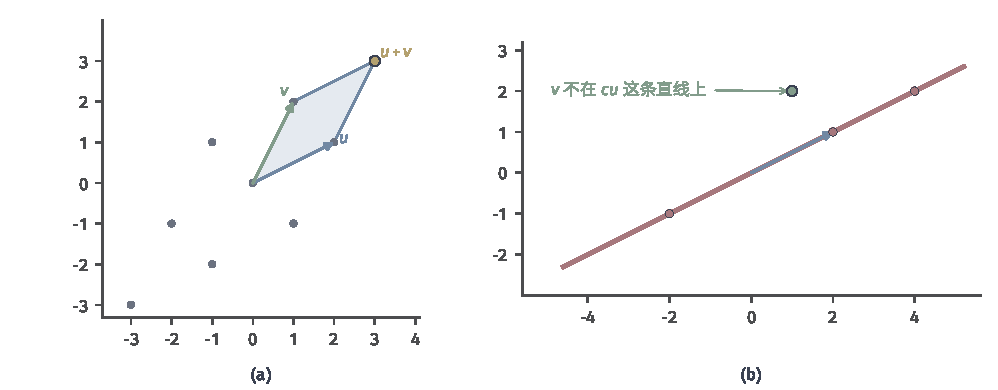
\includegraphics[width=169mm]{figures/00-shared/mathematical-preliminaries-upper/02-linear-spaces/matplotlib/ls-linear-combination-span/ls-linear-combination-span.pdf}
  \caption{两个方向与一个方向的张成范围。左：$\bm u=(2,1)$（蓝箭头）与$\bm v=(1,2)$（绿箭头）的全部加权组合取遍整个平面，浅蓝平行四边形标出$0,\bm u,\bm u+\bm v,\bm v$，灰点为整数系数格点，黄点为$\bm u+\bm v=(3,3)$。右：只有$\bm u$一个方向时，组合$\{c\bm u\}$只是过原点的一条直线（红线），$\bm v$不在其上。两图坐标等比例，为解析教学例。}
  \label{fig:ls-linear-combination-span}
\end{figure*}

\paragraph{线性无关}
\phantomsection
\label{sec:ls-linear-dependence}
张成回答“能表示哪些向量”，却不管“表示的方法有几种”。

先看一个平面上的例子。取
\[
 \bm u=(1,0)^\top,\qquad \bm v=(1,1)^\top,\qquad \bm w=(2,1)^\top .
\]
目标$(3,2)^\top$有两种写法：
\[
 (3,2)^\top=\bm u+2\bm v=\bm v+\bm w,
\]
两组系数$(1,2,0)$与$(0,1,1)$不同。原因是$\bm w=\bm u+\bm v$：$\bm w$能到达的地方，$\bm u$和$\bm v$合起来已经能到达，它没有带来新方向，只让系数多了一种选法。

把两种写法相减，得到
\[
 \bm u+\bm v-\bm w=\bm0 .
\]
这说明了一般规律：同一个向量若有两种不同的表示，相减就得到零向量的一个系数不全为零的表示；反过来，若零向量有这样的表示，把它加到任何一个表示上，就得到另一种表示。所以，要判断一组向量有没有多余的方向，只需看能否用不全为零的系数把它们组合成零向量。

据此给出定义。若
\begin{equation}
 a_1\bm v_1+\cdots+a_k\bm v_k=\bm0
 \label{eq:linear-algebra-independence-relation}
\end{equation}
只在$a_1=\cdots=a_k=0$时成立，就称$\bm v_1,\ldots,\bm v_k$\term{线性无关}（linearly independent）；否则称为\term{线性相关}（linearly dependent），即存在不全为零的系数使式~\eqref{eq:linear-algebra-independence-relation}成立。直观地说，线性无关就是“谁也不能被其余的向量凑出来”。

线性相关时，取一个非零系数$a_j$移项，就把$\bm v_j$写成其余向量的组合，如上例的$\bm w=\bm u+\bm v$；反之亦然。所以线性相关就是有某个向量多余，删去它不改变张成空间。

特别地，含零向量的组总是线性相关，两个向量线性相关当且仅当共线。在$\mathbb R^m$中，把向量排成矩阵$\bm V$的各列，线性无关就是$\bm V\bm a=\bm0$只有零解。上例的
\[
 \bm V=\begin{bmatrix}1&1&2\\0&1&1\end{bmatrix}
\]
有非零解$(1,1,-1)^\top$。

贯穿例中设计矩阵的两列几乎同向。它们是否线性无关，不能凭“看起来差不多”判断，要按定义检验。
\begin{example}[近共线的两列仍线性无关]
\label{ex:ls-nearly-collinear-independence}
式~\eqref{eq:linear-algebra-nearly-collinear-design}中的两列是$\bm c_1=(1,1,1)^\top$与$\bm c_2=\bm c_1+\varepsilon\bm q$，其中$\bm q=(0,1,-1)^\top$。$\bm c_2$由$\bm c_1$沿$\bm q$偏离一点得到，所以先确认$\bm c_1$与$\bm q$本身线性无关。二者的组合为
\[
 \alpha\bm c_1+\beta\bm q=(\alpha,\ \alpha+\beta,\ \alpha-\beta)^\top ,
\]
它为零时，第一坐标给出$\alpha=0$，第二坐标再给出$\beta=0$。

再把两列的组合改写到$\bm c_1,\bm q$上：
\[
 a_1\bm c_1+a_2\bm c_2=(a_1+a_2)\bm c_1+a_2\varepsilon\bm q .
\]
它为零时，由$\bm c_1,\bm q$线性无关，两个系数都须为零，即
\[
 a_1+a_2=0,\qquad a_2\varepsilon=0 .
\]
只要$\varepsilon\neq0$，第二式就迫使$a_2=0$，进而$a_1=0$，两列线性无关。只有$\varepsilon=0$时两列重合，$\bm c_1-\bm c_2=\bm0$，才线性相关。
\end{example}
因此，“几乎同向”与线性无关是两回事。线性无关只回答“是”或“否”：只要$\varepsilon\neq0$，答案就是“是”，不管$\varepsilon$多小。两列接近到什么程度，要用夹角等度量另行描述。

\paragraph{表示的存在与唯一}
张成管表示是否存在，线性无关管表示是否唯一，两者互不包含。下面的例子在平面上把它们分开。
\begin{example}[足够、不够与冗余的方向组]
\label{ex:ls-redundant-spanning-set}
在$\mathbb R^2$中取$\bm v_1=(1,0)^{\top}$、$\bm v_2=(0,1)^{\top}$与$\bm v_3=(1,1)^{\top}$，比较三种方向组。

用$\bm v_1,\bm v_2$两个方向时，$a_1\bm v_1+a_2\bm v_2=(a_1,a_2)^{\top}$，任一目标点$(x,y)^\top$都能取到，而且系数只能是$a_1=x$、$a_2=y$：方向既足够，又没有冗余。

只用$\bm v_1$时，组合$a_1\bm v_1=(a_1,0)^\top$停在横轴上，连$\bm v_2$都取不到：表示不一定存在。

三个方向一起用时，能到达的仍是整个平面，但$\bm v_3=\bm v_1+\bm v_2$，同一个目标有不同的系数，例如$(1,1)^\top$既是$\bm v_3$，又是$\bm v_1+\bm v_2$：表示存在，但不唯一。
\end{example}
图~\ref{fig:vol1-add-linear-redundant-directions}把第三种情形下的两种表示画在同一个平面上。
\begin{figure}[!htb]
  \centering
  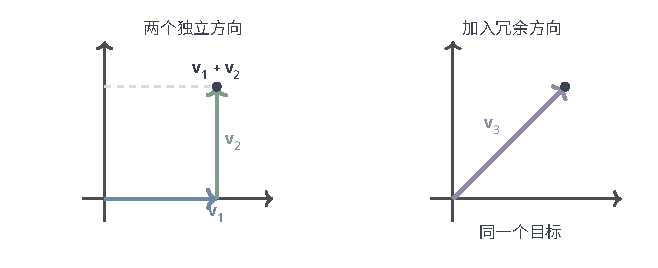
\includegraphics[width=112mm]{figures/00-shared/mathematical-preliminaries-upper/02-linear-spaces/tikz/comprehension-additions/linear-redundant-directions.pdf}
  \caption{冗余方向与重复表示。取$\bm v_1=(1,0)^{\top}$、$\bm v_2=(0,1)^{\top}$与$\bm v_3=(1,1)^{\top}$。左图沿$\bm v_1$再沿$\bm v_2$，右图直接沿$\bm v_3$，到达同一个目标；前两个向量已能表示平面中的每个向量，加入$\bm v_3$只使生成组冗余。两图坐标等比例。}
  \label{fig:vol1-add-linear-redundant-directions}
\end{figure}

一般地，张成保证每个向量都有表示；线性无关保证表示唯一，并且由上一段，表示唯一也反过来推出线性无关。后面定义坐标正以此为依据。

\subsection{基与维数}
\label{sec:ls-basis-dimension}

张成保证表示存在，线性无关保证表示唯一。同时满足这两个条件的一组向量称为\term{基}（basis）：它能到达整个空间，又没有多余的方向，可以充当整个空间的一把“尺子”。

$\mathbb R^d$的标准坐标向量$\bm e_1,\ldots,\bm e_d$是一组基，称为标准基：$\bm x=\sum_jx_j\bm e_j$说明它们张成$\mathbb R^d$，而$\sum_ja_j\bm e_j=(a_1,\ldots,a_d)^\top=\bm0$迫使全部$a_j=0$。

$P_k$中的$1,t,\ldots,t^k$也是一组基：每个多项式都是它们的组合，组合为零多项式时各项系数都为零。

子空间也有基。下面为一个齐次方程的解集合求出一组基。
\begin{example}[齐次方程解平面的一组基]
\label{ex:ls-solution-plane-basis}
设$N$是$\mathbb R^3$中齐次方程$x_1+2x_2+3x_3=0$的解集合；由示例~\ref{ex:ls-subspace-checks}，$N$是子空间。方程只约束了$x_1$：解满足
\[
 x_1=-2x_2-3x_3,
\]
而$x_2,x_3$可以任取。把每个解按这两个自由坐标拆开，
\[
 \bm x=x_2(-2,1,0)^\top+x_3(-3,0,1)^\top ,
\]
可见$\bm n_1=(-2,1,0)^\top$与$\bm n_2=(-3,0,1)^\top$张成$N$。

还要检查这两个方向没有冗余。若
\[
 a\bm n_1+b\bm n_2=(-2a-3b,\ a,\ b)^\top=\bm0,
\]
第二、三个坐标直接给出$a=b=0$，所以二者线性无关。于是$\bm n_1,\bm n_2$是$N$的一组基：两个自由坐标各对应一个基向量。
\end{example}

\paragraph{基的抽取与扩充}
若$V$有一个有限的生成组，就称$V$是有限维的；本章只讨论有限维空间。有限维空间总有基，可以从两个方向得到。

第一种做法是抽取。从任一有限生成组出发，若某个成员能写成其余向量的线性组合，删去它不会缩小张成范围。反复删除，直到剩下的向量中没有一个能由其余向量表示。这时剩下的向量线性无关，又仍张成$V$，构成一组基。

第二种做法是扩充。从任一线性无关组出发，逐次加入不在其张成空间中的向量。每加入一个新向量，张成范围严格扩大，新组仍线性无关。理由如下：若新组的某个组合为零，新向量的系数必为零，否则新向量能由原组表示，落在原张成空间中；新向量的系数为零以后，原组的线性无关性又使其余系数为零。

扩充不会无限进行下去。下文的交换引理（定理~\ref{thm:ls-exchange-lemma}）说明，有限维空间中线性无关组的长度不超过任一生成组的长度，所以扩充必在有限步内停止。停止时张成空间之外再没有向量，所得的组就是基。

抽取把冗余的生成组压缩成基，扩充把线性无关组补足成基。后面的许多证明都会用到扩充。

\paragraph{维数}
\label{sec:ls-dimension}

基的向量个数可以度量空间的大小，前提是换一组基时个数不变。这由交换引理保证。
\begin{theorem}[交换引理]
\label{thm:ls-exchange-lemma}
若$\bm u_1,\ldots,\bm u_r$线性无关，且每个$\bm u_i$都属于$\operatorname{span}\{\bm v_1,\ldots,\bm v_s\}$，则$r\leq s$；并且这$r$个$\bm u_i$可以逐个换入原生成组、换出同样多个$\bm v_j$，每次换完新组仍张成原来的空间。
\end{theorem}
\begin{proof}
从生成组$G_0=\{\bm v_1,\ldots,\bm v_s\}$开始。

因为$\bm u_1\in\operatorname{span}G_0$，它可写成若干$\bm v_j$的组合。这些系数不全为零，否则$\bm u_1=\bm0$，与$\bm u_1,\ldots,\bm u_r$线性无关矛盾。

取某个系数非零的$\bm v_j$，从这个表达式中把它解出，$\bm v_j$就能由$\bm u_1$与其余的$\bm v$表示。于是用$\bm u_1$换出$\bm v_j$，新组$G_1$与$G_0$张成同一个空间。

一般地，设第$i-1$步后的组$G_{i-1}$由$\bm u_1,\ldots,\bm u_{i-1}$和$s-(i-1)$个留下的$\bm v$组成，且与$G_0$张成同一空间。于是$\bm u_i\in\operatorname{span}G_{i-1}$。若$\bm u_i$只用$\bm u_1,\ldots,\bm u_{i-1}$就能表示，就违反线性无关；所以表达式中至少有一个留下的$\bm v$系数非零。把它解出并换入$\bm u_i$，张成范围不变。只要还有留下的$\bm v$，这一步就能继续。

若$r>s$，换满$s$次以后组内只剩$\bm u_1,\ldots,\bm u_s$，而$\bm u_{s+1}$属于$\operatorname{span}G_s=\operatorname{span}\{\bm u_1,\ldots,\bm u_s\}$，与$r$个$\bm u$线性无关矛盾。

故$r\leq s$，上面的逐次交换就是定理所说的换入换出过程。
\end{proof}

由交换引理，基的向量个数与基的选取无关。任取两组基，设个数分别为$r$与$s$。把第一组看成线性无关组、第二组看成生成组，得$r\leq s$；互换两组的角色，又得$s\leq r$，所以$r=s$。

这个共同的个数称为空间的\term{维数}（dimension），记为$\dim V$。只含零向量的空间以空集为基，维数为$0$。

交换引理的论证依赖有限的生成组，所以后面的基扩充与维数计算都限于有限维空间，不能直接用于无限维的函数展开。

\subsection{子空间的维数与分解}
有了维数，就能比较子空间的大小。若$U\subseteq W$，取$U$的一组基，它在$W$中仍线性无关，可以按上一小节的方法扩充成$W$的基。扩充只增加向量，所以$\dim U\leq\dim W$；新增向量的个数恰为$\dim W-\dim U$，它表示$U$之外还有多少个独立方向。

若同时有$\dim U=\dim W$，把$U$的基扩充成$W$的基不需要新增向量，即$U$的基已经张成$W$，所以$U=W$。这里的包含条件不能省略，仅凭维数相同推不出包含。
\begin{example}[反例：同维而互不包含的两条直线]
\label{ex:ls-equal-dimension-not-nested}
在$\mathbb R^2$中取横轴$U=\{(s,0)^\top:s\in\mathbb R\}$与对角线$W=\{(s,s)^\top:s\in\mathbb R\}$。二者分别以$\bm e_1$与$(1,1)^\top$为基，所以$\dim U=\dim W=1$。

然而$\bm e_1$的两个坐标不相等，不在$W$中；$(1,1)^\top$的第二坐标不为零，也不在$U$中。

两条直线维数相同，却互不包含。维数只数方向的个数，不记录这些方向指向哪里，所以上面的结论必须以$U\subseteq W$为前提。
\end{example}
“先取已有的基，再补新方向”这一做法，下面计算和空间、补空间与商空间时都会用到，后面的秩零度定理也以它为证明思路。

\paragraph{和空间}
两个子空间的公共方向在两边各计一次，所以和空间的维数一般小于两边维数之和。下面从交的一组基出发，算出准确的公式。

设$\bm z_1,\ldots,\bm z_k$是$U\cap W$的一组基，把它扩充为$U$的基$\bm z_1,\ldots,\bm z_k,\bm u_1,\ldots,\bm u_p$，再另行扩充为$W$的基$\bm z_1,\ldots,\bm z_k,\bm w_1,\ldots,\bm w_q$。我们说明这$k+p+q$个向量构成$U+W$的基。

每个$\bm u+\bm w$（$\bm u\in U$，$\bm w\in W$）都是这些向量的组合，所以它们张成$U+W$。为证线性无关，设
\[
 \sum_i\alpha_i\bm z_i+\sum_j\beta_j\bm u_j+\sum_l\gamma_l\bm w_l=\bm0 .
\]
移项得
\[
 \sum_l\gamma_l\bm w_l=-\sum_i\alpha_i\bm z_i-\sum_j\beta_j\bm u_j .
\]
左边属于$W$，右边属于$U$，所以这个向量属于$U\cap W$，可以写成$\sum_i\delta_i\bm z_i$。于是
\[
 \sum_l\gamma_l\bm w_l-\sum_i\delta_i\bm z_i=\bm0,
\]
由$W$的基线性无关，全部$\gamma_l=0$。代回原式，再由$U$的基线性无关，全部$\alpha_i$与$\beta_j$也为零。

因此
\[
 \dim(U+W)=k+p+q=(k+p)+(k+q)-k,
\]
即
\begin{equation}
 \dim(U+W)=\dim U+\dim W-\dim(U\cap W).
 \label{eq:ls-dimension-formula}
\end{equation}
减去的是两边重复计入的公共方向的个数，不是两个集合元素个数之差。下面在$\mathbb R^3$中核对这一公式。
\begin{example}[两个坐标平面的和]
\label{ex:ls-dimension-formula-planes}
在$\mathbb R^3$中取两个坐标平面$U=\operatorname{span}\{\bm e_1,\bm e_2\}$与$W=\operatorname{span}\{\bm e_2,\bm e_3\}$，维数都是$2$。

先求交：$U$由第三坐标为零的向量组成，$W$由第一坐标为零的向量组成，同时满足两条的向量只剩第二坐标，所以$U\cap W=\operatorname{span}\{\bm e_2\}$，维数为$1$。

再看和：$U+W$含有$\bm e_1,\bm e_2,\bm e_3$，所以就是$\mathbb R^3$。两边与公式相符：
\[
 \dim(U+W)=3=2+2-1 .
\]
减去的$1$正是两个平面共有的$\bm e_2$方向，它在$\dim U$与$\dim W$中各计了一次。

作为对照，改取两条坐标轴$U'=\operatorname{span}\{\bm e_1\}$、$W'=\operatorname{span}\{\bm e_2\}$。它们没有公共的非零向量，交为零，于是
\[
 \dim(U'+W')=1+1-0=2 .
\]
交为零时，和的维数等于两边维数之和。
\end{example}

\paragraph{补空间}
第~\ref{sec:ls-direct-sum}节定义了补空间，现在用基扩充证明它总存在。把$U$的基扩充为$V$的基，新增向量张成的子空间记为$W$。整组基张成$V$，所以$U+W=V$。

若某个向量同属$U$与$W$，它既是$U$的基向量的组合，又是新增向量的组合；两种写法相减，得到整组基的一个组合为零，所以系数全为零，该向量为零。于是$U\cap W=\{\bm0\}$，$V=U\oplus W$。

由维数公式，直和时交的维数为零，所以$\dim V=\dim U+\dim W$。扩充的方式不唯一，补空间也就不唯一，这与平面中直线的例子一致。

\paragraph{商空间}
同样的扩充也给出第~\ref{sec:ls-quotient-spaces}节商空间的维数。取$U$的一组基$\bm u_1,\ldots,\bm u_s$，扩充为$V$的基$\bm u_1,\ldots,\bm u_s,\bm w_1,\ldots,\bm w_t$。新增向量的类$\bm w_1+U,\ldots,\bm w_t+U$张成$V/U$：任一$\bm x$写成整组基的组合，其中属于$U$的部分落进零类而消去。

这些类也线性无关。若$\sum_ja_j(\bm w_j+U)=U$，则$\sum_ja_j\bm w_j\in U$，它能由$\bm u_i$表示，整组基的线性无关性迫使全部$a_j=0$。因此
\begin{equation}
 \dim(V/U)=\dim V-\dim U.
 \label{eq:ls-quotient-dimension}
\end{equation}

商空间的维数等于补空间的维数，二者的关系还可以说得更具体。新增向量$\bm w_j$张成$U$的一个补空间$W$，每个$\bm x$唯一分解为
\[
 \bm x=\bm u+\bm w,\qquad \bm u\in U,\ \bm w\in W,
\]
于是类$\bm x+U=\bm w+U$中的点都形如$\bm w+\bm u'$（$\bm u'\in U$）。这样的点落在$W$中，当且仅当$\bm u'\in U\cap W=\{\bm0\}$，所以每个类与$W$恰交于一点$\bm w$。

选定一个补空间，就是为每个类选定一个代表元。补空间需要选择，商空间不依赖任何选择，这是二者的区别。

在示例~\ref{ex:ls-quotient-intercept}中，$\dim(P_1/U)=2-1=1$，商空间只剩截距这一个方向；在图~\ref{fig:ls-quotient-equivalence-classes}中，$\dim(\mathbb R^2/U)=1$，只剩高度。

\subsection{坐标与坐标变换}
\label{sec:ls-coordinates}
\label{sec:linear-algebra-coordinates}

有了基，每个对象都有唯一的一组系数。本小节先把这组系数定义为坐标，说明它怎样代替对象参与计算；再看坐标的大小为什么不能直接反映对象的大小；最后推导换基时坐标的换算规则。

\paragraph{有序基下的坐标}
固定有序基$\mathcal B=(\bm b_1,\ldots,\bm b_d)$后，对象$\bm v$唯一写成$\sum_{j=1}^d x_j\bm b_j$。系数列$[\bm v]_{\mathcal B}=(x_1,\ldots,x_d)^{\top}$称为$\bm v$在基$\mathcal B$下的\term{坐标}（coordinates）。

由于存在性来自张成、唯一性来自线性无关，坐标映射$\bm v\mapsto[\bm v]_{\mathcal B}$是从$V$到$\mathbb R^d$的双射：每个对象恰有一列坐标，每列实数$(x_1,\ldots,x_d)^{\top}$也恰好记录对象$\sum_jx_j\bm b_j$。

坐标映射还保持线性组合。若$[\bm v]_{\mathcal B}=\bm x$、$[\bm w]_{\mathcal B}=\bm y$，则$a\bm v+b\bm w=\sum_j(ax_j+by_j)\bm b_j$，由唯一性得
\[
 [a\bm v+b\bm w]_{\mathcal B}=a\bm x+b\bm y.
\]
因此，对象上的线性运算可以完全在坐标上进行，算完再按基还原。

在$\mathbb R^d$中，把基向量排成矩阵$\bm B=[\bm b_1\ \cdots\ \bm b_d]$。按列读法，$\bm v=\bm B[\bm v]_{\mathcal B}$，所以坐标就是方程$\bm B\bm x=\bm v$的唯一解。下面用这个方程求一个斜基下的坐标。
\begin{example}[同一向量在两组基下的坐标]
\label{ex:ls-coordinates-two-bases}
取$\mathbb R^2$中的向量$\bm x=(1,2)^\top$。在标准基$(\bm e_1,\bm e_2)$下，$\bm x=1\cdot\bm e_1+2\cdot\bm e_2$，坐标就是$(1,2)^\top$。改用斜基$\mathcal B=(\bm b_1,\bm b_2)$，其中$\bm b_1=(2,1)^\top$、$\bm b_2=(-1,1)^\top$，坐标$(c_1,c_2)^\top$要由$c_1\bm b_1+c_2\bm b_2=\bm x$解出，逐坐标写开就是
\[
 \begin{gathered}
2c_1-c_2=1\\
c_1+c_2=2 .
 \end{gathered}
\]
两式相加消去$c_2$，得$3c_1=3$，所以$c_1=1$，再代入第二式得$c_2=1$。代回检验，
\[
 \bm b_1+\bm b_2=(1,2)^\top
\]
正是$\bm x$。

所以$[\bm x]_{\mathcal B}=(1,1)^\top$。向量本身没有移动，只是换了一组基来度量，读数随之改变。
\end{example}
图~\ref{fig:ls-basis-coordinates}画出这两种读法。
\begin{figure*}[htbp]
  \centering
  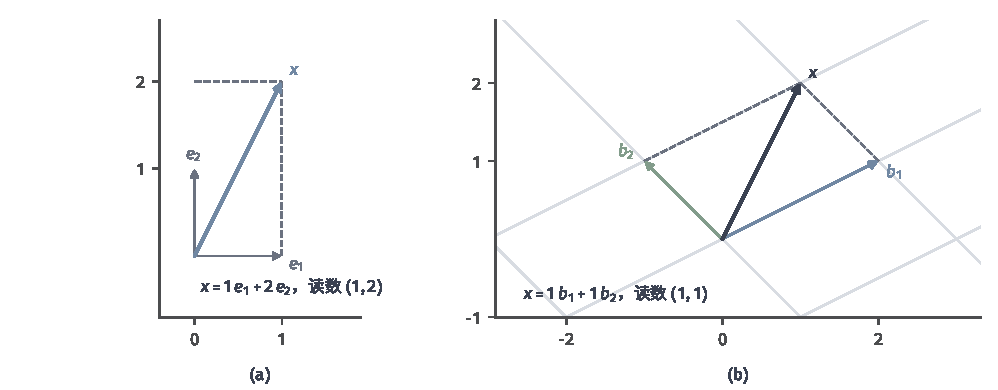
\includegraphics[width=169mm]{figures/00-shared/mathematical-preliminaries-upper/02-linear-spaces/matplotlib/ls-basis-coordinates/ls-basis-coordinates.pdf}
  \caption{同一向量在两组基下的坐标。左：标准基$\bm e_1,\bm e_2$（灰箭头）下，向量$\bm x=(1,2)$（蓝箭头）的坐标为$(1,2)$，虚线为向坐标轴的垂线。右：斜基$\bm b_1=(2,1)$（蓝）、$\bm b_2=(-1,1)$（绿）下，同一个$\bm x$满足$\bm x=\bm b_1+\bm b_2$，坐标为$(1,1)$，浅色斜线为斜基网格，虚线为平行四边形读法。两图坐标系相同。}
  \label{fig:ls-basis-coordinates}
\end{figure*}

\paragraph{坐标与对象}
坐标要与它记录的对象区分开。几何位移、有限信号、多项式都可以相加和缩放，它们是\emph{对象}；一列实数只是选定基以后记录对象的\emph{坐标}。基的顺序也要固定：交换$\bm b_1,\bm b_2$，对象不变，坐标列的前两个数随之交换。

在$\mathbb R^d$中直接写一列数，通常默认使用标准基$\bm e_1,\ldots,\bm e_d$，这时对象与坐标恰好是同一列数。第~\ref{chap:linear-operations}章就是在这种默认下工作的。

对函数的基展开，二者必须分开：函数是对象，展开系数是坐标。
\begin{example}[仿射函数在两组基下的坐标]
\label{ex:ls-affine-function-coordinates}
在$P_1$中用两组基记录同一个仿射函数$f_{a,b}=a+bt$。在$\mathcal B_1=(1,t)$下，$f_{a,b}=a\cdot1+b\cdot t$，坐标就是截距与斜率$(a,b)^\top$。

换成$\mathcal B_2=(1,1+t)$，设
\[
 f_{a,b}=c_1\cdot1+c_2(1+t)=(c_1+c_2)+c_2t ;
\]
比较$t$的系数得$c_2=b$，再比较常数项得$c_1=a-b$，即
\[
 f_{a,b}=(a-b)\cdot1+b\cdot(1+t).
\]
同一个函数在$\mathcal B_1$与$\mathcal B_2$下的坐标分别是$(a,b)^\top$与$(a-b,b)^\top$。坐标改变了，函数本身没有改变；“截距是第一个坐标”只在$\mathcal B_1$下成立。
\end{example}
坐标的个数总等于维数。若用冗余的生成组记录对象，记录的长度可以超过维数，所以不能由这种记录的长度推断空间的维数。

\paragraph{坐标对基的敏感性}
对象不变时，不同基下的坐标仍可能相差很大。贯穿例给出一个极端的情形。
\begin{example}[近共线基下的大坐标]
\label{ex:ls-coordinate-instability}
沿用示例~\ref{ex:ls-nearly-collinear-independence}中的$\bm c_1,\bm q$与$\bm c_2=\bm c_1+\varepsilon\bm q$（$\varepsilon\neq0$），并取$\delta=0.1$与目标向量
\begin{equation}
 \bm y=\bm c_1+\delta\bm q=\begin{bmatrix}1\\1.1\\0.9\end{bmatrix}.
 \label{eq:linear-algebra-nearly-collinear-target}
\end{equation}
由该示例，$\mathcal B_0=(\bm c_1,\bm q)$与$\mathcal B_\varepsilon=(\bm c_1,\bm c_2)$都是平面$\operatorname{span}\{\bm c_1,\bm q\}$的基，$\bm y$也在这个平面中，所以可以比较它在两组基下的坐标。

在$\mathcal B_0$下，$\bm y$的坐标直接读出为$(1,\delta)^{\top}$。要换到$\mathcal B_\varepsilon$，先由$\bm c_2=\bm c_1+\varepsilon\bm q$解出$\bm q=(\bm c_2-\bm c_1)/\varepsilon$，再代入$\bm y=\bm c_1+\delta\bm q$，得
\begin{equation}
 \bm y=\left(1-\frac{\delta}{\varepsilon}\right)\bm c_1
       +\frac{\delta}{\varepsilon}\bm c_2.
 \label{eq:linear-algebra-coordinate-instability}
\end{equation}
两个系数都含因子$\delta/\varepsilon$，$\varepsilon$越小，坐标越大。取$\varepsilon=0.01$，则$\delta/\varepsilon=10$，坐标成为$(-9,10)^{\top}$。

于是同一个$\bm y$在两组基下的坐标为
\[
 [\bm y]_{\mathcal B_0}=(1,0.1)^\top,\qquad [\bm y]_{\mathcal B_{0.01}}=(-9,10)^\top,
\]
第二个分量从$0.1$变成了$10$。
\end{example}
两个很大的系数作用在几乎同向的两个基向量上，大部分相互抵消，所以不能据此判断$\bm y$很大。坐标对接近退化的基的这种敏感性，第~\ref{chap:condition-and-spectral-perturbation}章将用条件数定量讨论。要系统地比较新旧坐标，先要建立换基的一般公式。

\paragraph{换基矩阵}
\phantomsection
\label{sec:ls-change-basis}
\label{sec:linear-algebra-coordinate-conversions}
设$\mathcal B=(\bm b_1,\ldots,\bm b_d)$与$\mathcal C$是$V$的两组有序基，已知$\bm v$在$\mathcal B$下的坐标$[\bm v]_{\mathcal B}=(x_1,\ldots,x_d)^{\top}$，要求它在$\mathcal C$下的坐标。由$\bm v=\sum_jx_j\bm b_j$，并且坐标映射保持线性组合，
\[
 [\bm v]_{\mathcal C}=\sum_{j=1}^d x_j[\bm b_j]_{\mathcal C}.
\]
右边是各列$[\bm b_j]_{\mathcal C}$以$x_j$为权重的线性组合。把这些列排成矩阵，称为从$\mathcal B$到$\mathcal C$的换基矩阵$\bm S_{\mathcal C\leftarrow\mathcal B}$。按矩阵与向量乘积的列读法，
\begin{equation}
 [\bm v]_{\mathcal C}
 =\bm S_{\mathcal C\leftarrow\mathcal B}[\bm v]_{\mathcal B}.
 \label{eq:linear-algebra-coordinate-change}
\end{equation}
换基矩阵的第$j$列是旧基向量$\bm b_j$的新坐标。下标$\mathcal C\leftarrow\mathcal B$从右向左读，表示把$\mathcal B$坐标换算成$\mathcal C$坐标。下面在平面上算一个具体的换基矩阵。
\begin{example}[平面上的换基矩阵]
\label{ex:ls-change-of-basis-plane}
设$\mathbb R^2$中的向量$\bm v$在基$\mathcal U=(\bm u_1,\bm u_2)$下的坐标为$(1,1)^\top$，其中$\bm u_1=(1,0)^{\top}$、$\bm u_2=(1,1)^{\top}$，要求它在标准基$\mathcal E$下的坐标。这里$\mathcal U$是旧基，$\mathcal E$是新基；$\bm u_1,\bm u_2$的标准坐标就是它们自己，按“第$j$列是旧基向量的新坐标”排成
\[
 \bm S_{\mathcal E\leftarrow\mathcal U}=\begin{bmatrix}1&1\\0&1\end{bmatrix}.
\]
由式~\eqref{eq:linear-algebra-coordinate-change}，
\[
 [\bm v]_{\mathcal E}=\bm S_{\mathcal E\leftarrow\mathcal U}(1,1)^{\top}=(2,1)^{\top}.
\]
不用换基矩阵也能得到同样结果：
\[
 \bm v=\bm u_1+\bm u_2=(2,1)^\top .
\]
所以$\mathcal U$坐标$(1,1)^\top$与标准坐标$(2,1)^\top$记录的是同一个向量。
\end{example}
图~\ref{fig:vol1-add-linear-change-basis}画出这一点：目标位置没有移动，改变的只是沿哪两个基方向累加，以及每个方向取多少份。
\begin{figure}[!htb]
  \centering
  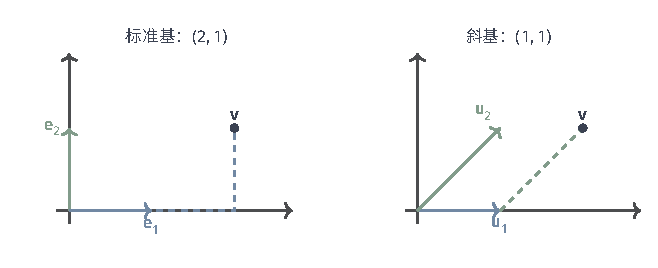
\includegraphics[width=112mm]{figures/00-shared/mathematical-preliminaries-upper/02-linear-spaces/tikz/comprehension-additions/linear-change-basis.pdf}
  \caption{同一向量的两套坐标。左图使用标准基，$\bm v=(2,1)^{\top}$的坐标为$(2,1)^{\top}$；右图使用$\bm u_1=(1,0)^{\top}$、$\bm u_2=(1,1)^{\top}$，同一$\bm v$的坐标为$(1,1)^{\top}$。虚线表示相应的向量相加，两图的环境坐标比例相同。}
  \label{fig:vol1-add-linear-change-basis}
\end{figure}

\paragraph{连续换基与反向换基}
连续换两次基，结果应与直接换基相同。设还有第三组基$\mathcal D$。对每个$\bm v$，连用两次式~\eqref{eq:linear-algebra-coordinate-change}，
\[
 \begin{aligned}
 [\bm v]_{\mathcal D}&=\bm S_{\mathcal D\leftarrow\mathcal C}[\bm v]_{\mathcal C}\\
 &=\bm S_{\mathcal D\leftarrow\mathcal C}\bm S_{\mathcal C\leftarrow\mathcal B}[\bm v]_{\mathcal B}.
 \end{aligned}
\]
取$\bm v=\bm b_j$，它的$\mathcal B$坐标是$\bm e_j$，两边读出的分别是$\bm S_{\mathcal D\leftarrow\mathcal B}$与乘积的第$j$列，所以
\[
 \bm S_{\mathcal D\leftarrow\mathcal B}
 =\bm S_{\mathcal D\leftarrow\mathcal C}\bm S_{\mathcal C\leftarrow\mathcal B}.
\]

特别取$\mathcal D=\mathcal B$。每个$\bm b_j$在$\mathcal B$下的坐标是$\bm e_j$，所以$\bm S_{\mathcal B\leftarrow\mathcal B}=\bm I_d$，即
\[
 \bm S_{\mathcal B\leftarrow\mathcal C}\bm S_{\mathcal C\leftarrow\mathcal B}=\bm I_d ;
\]
交换两组基的角色，同理得
\[
 \bm S_{\mathcal C\leftarrow\mathcal B}\bm S_{\mathcal B\leftarrow\mathcal C}=\bm I_d .
\]
所以换基矩阵总可逆，反向换基矩阵就是它的逆：
\[
 \bm S_{\mathcal B\leftarrow\mathcal C}=\bm S_{\mathcal C\leftarrow\mathcal B}^{-1}.
\]
在示例~\ref{ex:ls-change-of-basis-plane}中，
\[
 \bm S_{\mathcal U\leftarrow\mathcal E}=\bm S_{\mathcal E\leftarrow\mathcal U}^{-1}=\begin{bmatrix}1&-1\\0&1\end{bmatrix},
\]
它把$(2,1)^{\top}$送回$(1,1)^{\top}$。

反过来，任一$d$阶可逆矩阵$\bm P$都是某次换基的矩阵。以$\bm P$的第$j$列为$\mathcal B$坐标，取向量$\bm b'_j=\sum_i\bm P_{i,j}\bm b_i$。$\bm P$的列线性无关，而坐标映射是保持线性组合的双射，所以$\bm b'_1,\ldots,\bm b'_d$也线性无关。

个数等于维数的线性无关组必是基：否则它还能扩充，得到多于$\dim V$个线性无关的向量，与交换引理矛盾。于是$\bm b'_1,\ldots,\bm b'_d$构成一组基$\mathcal B'$。按定义，$\bm S_{\mathcal B\leftarrow\mathcal B'}$的第$j$列是$\bm b'_j$的$\mathcal B$坐标，即$\bm P$的第$j$列，所以$\bm S_{\mathcal B\leftarrow\mathcal B'}=\bm P$。

换基矩阵接近不可逆时，反向换基会放大坐标。贯穿例清楚地显示了这一点。
\begin{example}[近共线基之间的换基]
\label{ex:ls-nearly-collinear-change-of-basis}
回到示例~\ref{ex:ls-coordinate-instability}中的两组基$\mathcal B_0=(\bm c_1,\bm q)$与$\mathcal B_\varepsilon=(\bm c_1,\bm c_2)$，$\varepsilon\neq0$，用换基矩阵重做那里的坐标换算。由
\[
 \bm c_1=1\cdot\bm c_1+0\cdot\bm q,\qquad \bm c_2=1\cdot\bm c_1+\varepsilon\bm q,
\]
$\mathcal B_\varepsilon$的两个向量在$\mathcal B_0$下的坐标分别是$(1,0)^{\top}$与$(1,\varepsilon)^{\top}$。以它们为列得到$\bm S_{\mathcal B_0\leftarrow\mathcal B_\varepsilon}$，求逆得到反方向的换基矩阵：
\[
\begin{gathered}
\bm S_{\mathcal B_0\leftarrow\mathcal B_\varepsilon}
 =\begin{bmatrix}1&1\\0&\varepsilon\end{bmatrix}\\
\bm S_{\mathcal B_\varepsilon\leftarrow\mathcal B_0}
 =\bm S_{\mathcal B_0\leftarrow\mathcal B_\varepsilon}^{-1}
 =\begin{bmatrix}1&-1/\varepsilon\\0&1/\varepsilon\end{bmatrix},
\end{gathered}
\]
逆矩阵可由两者相乘得单位矩阵验证。把$\bm y$在$\mathcal B_0$下的坐标$(1,\delta)^{\top}$代入后者，得
\[
 \bm S_{\mathcal B_\varepsilon\leftarrow\mathcal B_0}\begin{bmatrix}1\\\delta\end{bmatrix}
 =\begin{bmatrix}1-\delta/\varepsilon\\\delta/\varepsilon\end{bmatrix},
\]
与式~\eqref{eq:linear-algebra-coordinate-instability}一致。

放大的来源在矩阵上看得很清楚。$\bm S_{\mathcal B_0\leftarrow\mathcal B_\varepsilon}$的行列式为$\varepsilon$，接近零，矩阵接近不可逆；它的逆因而含有因子$1/\varepsilon$，两组基之间的微小差异由此被放大成大系数。
\end{example}

\paragraph{被动换基与主动作用}
换基公式与矩阵作用都写成矩阵乘以坐标列，但含义不同，必须分开。换基是被动的：对象不动，记录改变，式\eqref{eq:linear-algebra-coordinate-change}两侧是同一个$\bm v$的两套坐标。矩阵作用是主动的：坐标系不动，对象被送到另一个对象，例如第~\ref{chap:linear-operations}章的$\bm x\mapsto\bm A\bm x$把向量旋转或切变；下一节把这种作用推广为线性映射。下面的例子从同一个初始向量出发比较两种情形。
\begin{example}[被动换基与主动切变]
\label{ex:ls-passive-vs-active}
取$\mathbb R^2$中的向量$\bm x=(3,3)^\top$，分别对它作被动换基与主动切变。换基用斜基$\mathcal B'=(\bm b_1,\bm b_2)$，$\bm b_1=(2,1)^\top$、$\bm b_2=(-1,1)^\top$；切变用矩阵
\[
 \bm A=\begin{bmatrix}1&1\\0&1\end{bmatrix}.
\]

被动换基要求$\bm x$在$\mathcal B'$下的坐标$(c_1,c_2)^\top$。逐坐标写开得
\[
 \begin{gathered}
 2c_1-c_2=3\\
 c_1+c_2=3,
 \end{gathered}
\]
解得$c_1=2$、$c_2=1$，即$\bm x=2\bm b_1+\bm b_2$。这时向量仍是$(3,3)^\top$，只是读数从$(3,3)$变成$(2,1)$。

主动作用则在标准坐标下计算
\[
 \bm A\bm x=(3+3,\ 3)^\top=(6,3)^\top .
\]
这时坐标系不动，向量本身被搬到了另一个位置。
\end{example}
图~\ref{fig:ls-passive-change-vs-active-map}把两种情形并排画出。可见，并非所有乘矩阵的运算都是换基。
\begin{figure*}[htbp]
  \centering
  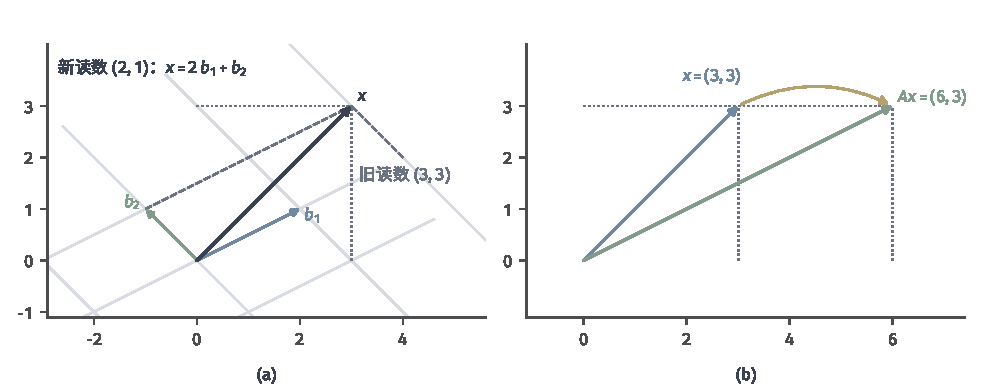
\includegraphics[width=169mm]{figures/00-shared/mathematical-preliminaries-upper/02-linear-spaces/matplotlib/ls-passive-change-vs-active-map/ls-passive-change-vs-active-map.pdf}
  \caption{被动换基与主动变换的对照，两图使用同一个初始向量$\bm x=(3,3)$。左（被动换基）：箭头位置不动（深色），旧标准读数用点线投影读出$(3,3)$；新斜基$\bm b_1=(2,1)$（蓝）、$\bm b_2=(-1,1)$（绿）与浅色斜网格下，$\bm x=2\bm b_1+\bm b_2$，新读数为$(2,1)$。右（主动变换）：标准坐标系不动，$\bm x$（蓝）被切变映到$\bm A\bm x=(6,3)$（绿），黄色弧线表示搬动过程。}
  \label{fig:ls-passive-change-vs-active-map}
\end{figure*}

% 第2章第3节：线性映射（定义；表示：矩阵表示、基于矩阵的映射运算、矩阵基本子空间；核与像、秩零度、商空间、行空间与列空间、可逆性；换基：相抵与相似；多线性映射）。

\section{线性与多线性映射}
\label{sec:ls-linear-maps}
\label{sec:linear-algebra-matrices-linear-maps}

前两节讨论单个空间中的对象怎样记录。本节转向对象之间保持线性组合的作用，即线性映射。选定两端的基，线性映射记成矩阵，映射的叠加、复合与求逆对应矩阵的加法、乘法与求逆。核与像分别描述映射消去的输入和能到达的输出，秩零度定理联系二者的维数，并由此给出可逆的判据。换基改变矩阵而不改变映射：两端各自换基得到相抵，算子两端同时换基得到相似。最后简述对每个输入分别线性的多线性映射。

\subsection{线性映射及其矩阵表示}
\label{sec:ls-linear-map-definition}
\label{sec:linear-algebra-maps}

设计矩阵把一组系数变成一列拟合值，求导把一个多项式变成另一个多项式，读取第一个坐标把向量变成一个数。这些作用有一个共同点：先把输入加权相加再作用，与先分别作用再作同样的加权相加，结果相同。有了这一性质，输入写成基向量的组合以后，作用的结果就是各基向量的像的同样组合，前两节的语言可以直接用于作用本身。保持线性组合的作用称为\term{线性映射}（linear map）$T:V\to W$：
\begin{equation}
T(a\bm x+b\bm y)=aT\bm x+bT\bm y,\qquad\bm x,\bm y\in V,\ a,b\in\mathbb R.
\label{eq:ls-linear-map-def}
\end{equation}
取$a=b=0$得$T\bm0=\bm0$，线性映射总把零向量送到零向量。由式~\eqref{eq:prelim-matrix-linearity}，任何矩阵$\bm A\in\mathbb R^{m\times d}$给出的$\bm x\mapsto\bm A\bm x$都是从$\mathbb R^d$到$\mathbb R^m$的线性映射。下面再检查几个作用是否线性。
\begin{example}[线性与非线性的作用]
\label{ex:ls-linear-map-checks}
考察下面三个作用：
\[
 \begin{aligned}
 &T:\mathbb R^2\to\mathbb R^2, &&T(x_1,x_2)=(2x_1+x_2,\ 3x_2);\\
 &D:P_k\to P_k, &&Dp=p';\\
 &\tau:\mathbb R\to\mathbb R, &&\tau(x)=x+1.
 \end{aligned}
\]
$T$的两个输出分量都是输入的加权和，写成矩阵就是
\[
 T\bm x=\begin{bmatrix}2&1\\0&3\end{bmatrix}\bm x,
\]
所以它是矩阵给出的映射，保持线性组合。求导满足$(ap+bq)'=ap'+bq'$，所以$D$也保持线性组合；又因为求导不升高次数，$D$确实把$P_k$送回$P_k$。

$\tau$看起来同样简单，却不是线性映射：$\tau(0)=1\neq0$，而线性映射必把$0$送到$0$。加上常数就把零点移走了，这与示例~\ref{ex:ls-subspace-checks}中平移后的直线不含零向量是同一类现象。
\end{example}

\phantomsection
\label{sec:ls-operator-powers}
输入与输出是同一个空间的线性映射$T:V\to V$称为\term{线性算子}（linear operator），也称线性变换。平面上的旋转、向一条直线的投影、$P_k$上的求导都是线性算子，示例~\ref{ex:ls-linear-map-checks}中的$T$也是。

输入与输出相同，使算子与一般映射有两点不同。第一，算子的输出仍在$V$中，可以再次作为输入，所以算子能与自身复合、反复作用。记$T^2=T\circ T$、$T^k=T\circ T^{k-1}$，并约定$T^0=\operatorname{id}_V$。一般映射$V\to W$在$V\neq W$时不能这样反复作用。后面将看到，在同一组基下，$T^k$的矩阵就是$T$的矩阵的$k$次幂。

第二，记录算子时，输入和输出可以用同一组基，这决定了算子换基时的特殊规律（第~\ref{sec:ls-similarity}节）。

\phantomsection
\label{sec:ls-map-representation}
线性映射的定义域通常有无穷多个元素，不可能逐个记录输出。选定基以后，有限个数就够了：在两端的固定基下，线性映射与矩阵一一对应，映射的叠加、复合与求逆分别对应矩阵的加法、乘法与求逆。第~\ref{chap:linear-operations}章的矩阵由此获得一般含义：矩阵是线性映射在坐标下的记录。下面先建立这一对应，再翻译映射的运算，最后定义矩阵的四个基本子空间，供下一小节使用。

\subsubsection{矩阵表示}

给定输入基$\mathcal B=(\bm b_1,\ldots,\bm b_d)$，任一$\bm v=\sum_jx_j\bm b_j$的像由线性性写成
\[
 T\bm v=\sum_{j=1}^d x_j\,T\bm b_j,
\]
所以只要知道$d$个基向量的像，整个映射就确定了。再给定输出基$\mathcal C$，把每个像的坐标$[T\bm b_j]_{\mathcal C}$作为第$j$列，排成矩阵$\bm A=[T]_{\mathcal C\leftarrow\mathcal B}\in\mathbb R^{m\times d}$，称为$T$在这两组基下的矩阵。

对上式两边取$\mathcal C$坐标，由坐标映射保持线性组合，并按矩阵与向量乘积的列读法，得到
\begin{equation}
 \begin{aligned}
 [T\bm v]_{\mathcal C}
 &=\sum_{j=1}^d x_j\,[T\bm b_j]_{\mathcal C}
 =\sum_{j=1}^d x_j\bm A_{:,j}\\
 &=[T]_{\mathcal C\leftarrow\mathcal B}\,[\bm v]_{\mathcal B}.
 \end{aligned}
 \label{eq:linear-algebra-map-matrix-representation}
\end{equation}
也就是说，输出坐标等于矩阵乘以输入坐标。作用在对象上进行，记录在坐标上进行，二者由矩阵与向量的乘积连接。

矩阵的列数是输入维数，行数是输出维数。下标$\mathcal C\leftarrow\mathcal B$从右向左读，表示输入用$\mathcal B$记录、输出用$\mathcal C$记录。算子的两端通常用同一组基，记为$[T]_{\mathcal B}=[T]_{\mathcal B\leftarrow\mathcal B}$，它是$\dim V$阶方阵。

下面按这一规则写出两个映射的矩阵。
\begin{example}[由基向量的像写出矩阵]
\label{ex:ls-plane-operator-matrix}
对示例~\ref{ex:ls-linear-map-checks}中的$T(x_1,x_2)=(2x_1+x_2,\ 3x_2)$，输入输出都取标准基。两个基向量的像是$T\bm e_1=(2,0)^{\top}$与$T\bm e_2=(1,3)^{\top}$，它们在标准基下的坐标就是自身。依次作为两列，得
\[
 [T]=\begin{bmatrix}2&1\\0&3\end{bmatrix}.
\]
这正是定义$T$时用的矩阵：按规则从基向量的像重建矩阵，没有丢失任何信息。
\end{example}
一般地，$\bm x\mapsto\bm A\bm x$在标准基下的矩阵就是$\bm A$本身，因为$\bm A\bm e_j=\bm A_{:,j}$。矩阵表示同样适用于不是数组的对象。
\begin{example}[求导的矩阵表示]
\label{ex:ls-derivative-matrix}
考虑求导$D:P_2\to P_2$，输入输出都取基$(1,t,t^2)$。三个基向量的导数是$D1=0$、$Dt=1$、$Dt^2=2t$，它们在这组基下的坐标依次为$(0,0,0)^\top$、$(1,0,0)^\top$、$(0,2,0)^\top$。以此为列，
\[
 [D]=\begin{bmatrix}0&1&0\\0&0&2\\0&0&0\end{bmatrix}.
\]
用一般的多项式检验这个矩阵。$p=a_0+a_1t+a_2t^2$的坐标是$(a_0,a_1,a_2)^\top$，而
\[
 [D](a_0,a_1,a_2)^\top=(a_1,2a_2,0)^\top,
\]
正是$p'=a_1+2a_2t$的坐标。对多项式求导，在坐标下就是乘矩阵$[D]$，尽管多项式本身不是一列数。
\end{example}

两个例子都是先有映射、再写矩阵。反过来，每个同形矩阵也都记录某个线性映射。
\begin{theorem}[线性映射与矩阵的对应]
\label{thm:ls-map-matrix-correspondence}
设$\dim V=d$、$\dim W=m$，并固定$V$的基$\mathcal B$与$W$的基$\mathcal C$。则$T\mapsto[T]_{\mathcal C\leftarrow\mathcal B}$是从全部线性映射$V\to W$到全部$m\times d$实矩阵的双射。
\end{theorem}
\begin{proof}
单射：若两个线性映射的矩阵相同，它们在每个基向量上的像相同，由$T\bm v=\sum_jx_jT\bm b_j$，它们在每个$\bm v$上都相同。

满射：任给$\bm A\in\mathbb R^{m\times d}$，对$\bm v\in V$令$T\bm v$为$\mathcal C$坐标等于$\bm A[\bm v]_{\mathcal B}$的那个向量。坐标唯一，所以这一规则有确定的意义；坐标映射与乘矩阵都保持线性组合，所以$T$线性；$T\bm b_j$的坐标是$\bm A\bm e_j=\bm A_{:,j}$，所以$[T]_{\mathcal C\leftarrow\mathcal B}=\bm A$。
\end{proof}
所以基固定以后，线性映射与矩阵一一对应；特别地，每个从$\mathbb R^d$到$\mathbb R^m$的线性映射在标准基下都是乘某个矩阵。这一对应依赖基的选取：改变两端任一组基，数表通常随之改变，记录的仍是同一个映射。数表怎样随基改变，在第~\ref{sec:ls-coordinates-change-of-basis}节推导。

设计矩阵$\bm X_\varepsilon$就是这样一张记录。它表示映射$T_\varepsilon:\mathbb R^2\to\mathbb R^3$，
\[
 \bm w\mapsto\bm X_\varepsilon\bm w=w_1\bm c_1+w_2\bm c_2,
\]
两列分别是两个输入基向量的像。输入是两个系数，输出是三个样本的拟合值，二者不在同一个空间中。图~\ref{fig:ch06-object-coordinate-map}概括了对象与坐标的关系：先作用于对象再取坐标，与先取输入坐标再乘矩阵，得到相同的输出坐标。
\begin{figure}[htbp]
  \centering
  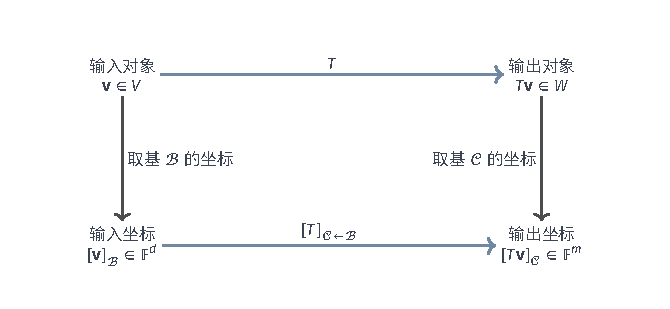
\includegraphics[width=112.0mm]{figures/00-shared/mathematical-preliminaries-upper/02-linear-spaces/tikz/ch06-object-coordinate-map/figure.pdf}
  \caption{先作用于对象再取坐标，与先取输入坐标再按矩阵的列作线性组合（即乘矩阵），得到相同输出坐标。横向箭头改变对象或数值，竖向箭头只改变记录方式。}
  \label{fig:ch06-object-coordinate-map}
\end{figure}

\subsubsection{基于矩阵的映射运算}
\phantomsection
\label{sec:ls-map-addition-composition}

映射之间有几种常用运算：把两个映射的输出相加，让两个映射接连作用，撤销一个映射。在固定基下，它们分别记录为第~\ref{chap:linear-operations}章的矩阵加法、乘法与求逆。带常数偏置的仿射映射不是线性映射，但可以借增广坐标写成一张更大的矩阵。

\paragraph{叠加}
\phantomsection
\label{sec:linear-algebra-map-addition}
设$T,S:V\to W$是同一对空间之间的两个线性映射，定义
\[
(aT+bS)(\bm x)=aT\bm x+bS\bm x,\qquad\bm x\in V,\ a,b\in\mathbb R.
\]

把输入的线性组合代入，两项分别展开再汇总，可知叠加仍是线性映射。在$V$与$W$的固定基下，设$T,S$的矩阵为$\bm A,\bm B$。$aT+bS$把第$j$个基向量送到$aT\bm b_j+bS\bm b_j$，其坐标是$a\bm A_{:,j}+b\bm B_{:,j}$，所以$aT+bS$的矩阵就是$a\bm A+b\bm B$。

相加要求两个映射的定义域相同、陪域也相同，这对应于只有同形矩阵才能相加。它不要求$V=W$：两个从$\mathbb R^2$到$\mathbb R^3$的映射可以相加，但不能与一个从$\mathbb R^3$到$\mathbb R^2$的映射相加。系数$a,b$必须与输入无关；若系数随$\bm x$改变，叠加的结果一般不再线性，需要单独检验。

\paragraph{复合}
设$T:U\to V$、$S:V\to W$是线性映射。复合$S\circ T$先作用$T$、再作用$S$，仍保持线性组合：
\[
 S(T(a\bm x+b\bm y))=S(aT\bm x+bT\bm y)=aS(T\bm x)+bS(T\bm y).
\]
取$U,V,W$的基$\mathcal B,\mathcal C,\mathcal D$。对每个$\bm x\in U$，两次使用式~\eqref{eq:linear-algebra-map-matrix-representation}，再用矩阵乘法的结合律，得
\[
 \begin{aligned}
 [S(T\bm x)]_{\mathcal D}
 &=[S]_{\mathcal D\leftarrow\mathcal C}[T\bm x]_{\mathcal C}\\
 &=[S]_{\mathcal D\leftarrow\mathcal C}\bigl([T]_{\mathcal C\leftarrow\mathcal B}[\bm x]_{\mathcal B}\bigr)\\
 &=\bigl([S]_{\mathcal D\leftarrow\mathcal C}[T]_{\mathcal C\leftarrow\mathcal B}\bigr)[\bm x]_{\mathcal B}.
 \end{aligned}
\]
取$\bm x=\bm b_j$，其坐标是$\bm e_j$，两边读出的是$[S\circ T]_{\mathcal D\leftarrow\mathcal B}$与乘积的第$j$列，所以
\begin{equation}
 [S\circ T]_{\mathcal D\leftarrow\mathcal B}
 =[S]_{\mathcal D\leftarrow\mathcal C}\,[T]_{\mathcal C\leftarrow\mathcal B}.
 \label{eq:ls-composition-matrix}
\end{equation}

复合的矩阵是矩阵的乘积，中间空间$V$的基$\mathcal C$在乘积中消去；第~\ref{sec:prelim-linear-actions-composition}节的推导是这里取标准基的特例。恒等映射$\operatorname{id}_V$在同一组基下的矩阵是单位矩阵。映射复合的结合律对应矩阵乘法的结合律；矩阵乘法不可交换，对应先后作用的次序不能交换。

对算子$T:V\to V$两端都用基$\mathcal B$，反复使用式~\eqref{eq:ls-composition-matrix}，得
\[
 [T^k]_{\mathcal B}=([T]_{\mathcal B})^k .
\]
算子的反复作用因此记录为第~\ref{sec:ls-matrix-power-rules}节的矩阵幂。例如对示例~\ref{ex:ls-derivative-matrix}中的$[D]$直接相乘可得$[D]^3=\bm0$，这对应于任何次数不超过$2$的多项式求导三次都变为零。

\paragraph{逆映射}
第~\ref{sec:prelim-inverse-matrices}节把满足$\bm A\bm B=\bm B\bm A=\bm I$的方阵$\bm A$称为可逆矩阵，那里只把它看成可以撤销的数表运算。有了矩阵表示，可以说明它记录的是哪一类映射。

若线性映射$T:V\to W$是双射，每个输出恰有一个原输入，逆映射$T^{-1}:W\to V$存在。逆映射自动是线性的：对$\bm w,\bm w'\in W$，由$T$的线性性
\[
 T\bigl(aT^{-1}\bm w+bT^{-1}\bm w'\bigr)=a\bm w+b\bm w',
\]
所以$aT^{-1}\bm w+bT^{-1}\bm w'$就是$a\bm w+b\bm w'$唯一的原输入，即
\[
 T^{-1}(a\bm w+b\bm w')=aT^{-1}\bm w+bT^{-1}\bm w'.
\]
这样的$T$称为可逆线性映射。

可逆映射与可逆矩阵相互对应。设$T:V\to W$可逆，在基$\mathcal B,\mathcal C$下$\bm A=[T]_{\mathcal C\leftarrow\mathcal B}$，$\bm B=[T^{-1}]_{\mathcal B\leftarrow\mathcal C}$。由式~\eqref{eq:ls-composition-matrix}，$T^{-1}\circ T=\operatorname{id}_V$与$T\circ T^{-1}=\operatorname{id}_W$分别给出$\bm B\bm A=\bm I$与$\bm A\bm B=\bm I$。所以$\bm A$是可逆方阵（下一小节将说明此时必有$\dim V=\dim W$），且$[T^{-1}]_{\mathcal B\leftarrow\mathcal C}=\bm A^{-1}$。

反过来，若$\bm A$可逆，$\bm y\mapsto\bm A^{-1}\bm y$就是$\bm x\mapsto\bm A\bm x$的逆映射。

两个可逆映射接连作用时，$(S\circ T)^{-1}=T^{-1}\circ S^{-1}$，在矩阵上就是式~\eqref{eq:ls-inverse-product}。判断一个映射是否可逆，要先知道它丢失了什么、能到达什么，这由下一小节处理。

\paragraph{仿射映射}
\phantomsection
\label{sec:ls-affine-maps}
线性模型的预测常带截距，平面上的平移也常与旋转一起出现，这些作用都不把原点留在原处。带常数偏置的规则$\bm x\mapsto\bm A\bm x+\bm b$称为\term{仿射映射}（affine map）。当$\bm b\neq\bm0$时，它把$\bm0$送到$\bm b$，所以不是线性映射；当$\bm b=\bm0$时，它就是线性映射。

两个仿射映射$\bm x\mapsto\bm A_1\bm x+\bm b_1$、$\bm y\mapsto\bm A_2\bm y+\bm b_2$复合，得到
\[
 \bm x\mapsto\bm A_2\bm A_1\bm x+(\bm A_2\bm b_1+\bm b_2),
\]
前一个映射的平移项也受到后一个映射的作用。

给坐标补一个恒为$1$的末位，仿射映射就能写成高一维空间上的线性作用：
\begin{equation}
 \begin{bmatrix}\bm A&\bm b\\ \bm0^\top&1\end{bmatrix}
 \begin{bmatrix}\bm x\\1\end{bmatrix}
 =
 \begin{bmatrix}\bm A\bm x+\bm b\\1\end{bmatrix}.
 \label{eq:ls-affine-homogeneous}
\end{equation}
按分块乘法，两个这样的增广矩阵相乘得
\[
 \begin{bmatrix}\bm A_2&\bm b_2\\ \bm0^\top&1\end{bmatrix}
 \begin{bmatrix}\bm A_1&\bm b_1\\ \bm0^\top&1\end{bmatrix}
 =\begin{bmatrix}\bm A_2\bm A_1&\bm A_2\bm b_1+\bm b_2\\ \bm0^\top&1\end{bmatrix},
\]
正是复合仿射映射的增广矩阵。

增广矩阵在整个增广空间上是线性的，但原输入只取末坐标为$1$的向量，所以不能据此说原映射线性。第~\ref{chap:linear-solution-selection}章用这种形式描述仿射解集的几何。

\subsubsection{矩阵基本子空间}
\phantomsection
\label{sec:ls-four-fundamental-subspaces}

矩阵$\bm A\in\mathbb R^{m\times d}$给出从$\mathbb R^d$到$\mathbb R^m$的映射$\bm x\mapsto\bm A\bm x$，它的转置$\bm A^\top\in\mathbb R^{d\times m}$给出反方向的映射$\bm y\mapsto\bm A^\top\bm y$。对每个方向可以问两个问题：哪些输出能够到达，哪些输入被送到零。四个答案都是子空间，它们刻画了矩阵保留和丢失的信息。

按矩阵与向量乘积的列读法，$\bm A\bm x=\sum_jx_j\bm A_{:,j}$。$\bm x$取遍$\mathbb R^d$时，输出取遍$\bm A$各列的全部线性组合，即各列的张成空间，称为$\bm A$的\term{列空间}（column space），记为$\operatorname{range}(\bm A)$。所以方程$\bm A\bm x=\bm b$有解，当且仅当$\bm b\in\operatorname{range}(\bm A)$。

齐次方程组$\bm A\bm x=\bm0$的解集合是$\mathbb R^d$的子空间（示例~\ref{ex:ls-subspace-checks}），称为$\bm A$的\term{零空间}（null space），记为$\operatorname{null}(\bm A)$。

对$\bm A^\top$问同样的两个问题，又得到两个子空间。$\bm A^\top$的列就是$\bm A$的行，所以$\operatorname{range}(\bm A^\top)$由$\bm A$各行的线性组合组成，称为$\bm A$的\term{行空间}（row space）。

$\bm A^\top\bm y=\bm0$转置后就是$\bm y^\top\bm A=\bm0^\top$，即$\bm y^\top$从左边乘$\bm A$得到零，所以$\operatorname{null}(\bm A^\top)$称为$\bm A$的\term{左零空间}（left null space）。

这四个子空间合称$\bm A$的\term{四个基本子空间}（four fundamental subspaces）：
\begin{equation}
 \begin{aligned}
  \operatorname{range}(\bm A)&=\{\bm A\bm x:\bm x\in\mathbb R^d\}\subseteq\mathbb R^m,\\
  \operatorname{null}(\bm A)&=\{\bm x\in\mathbb R^d:\bm A\bm x=\bm0\}\subseteq\mathbb R^d,\\
  \operatorname{range}(\bm A^\top)&=\{\bm A^\top\bm y:\bm y\in\mathbb R^m\}\subseteq\mathbb R^d,\\
  \operatorname{null}(\bm A^\top)&=\{\bm y\in\mathbb R^m:\bm A^\top\bm y=\bm0\}\subseteq\mathbb R^m.
 \end{aligned}
 \label{eq:ls-four-fundamental-subspaces}
\end{equation}

零空间与行空间在输入空间$\mathbb R^d$中，列空间与左零空间在输出空间$\mathbb R^m$中。零空间收集被完全消去的输入方向。

行空间收集读取输出分量所用的方向：输出的第$i$个分量$(\bm A\bm x)_i=\bm A_{i,:}\bm x$由第$i$行与$\bm x$逐项相乘再相加得到。

左零空间收集对可达输出读数恒为零的加权方式：对$\bm y\in\operatorname{null}(\bm A^\top)$与任意输入$\bm x$，
\[
 \bm y^\top(\bm A\bm x)=(\bm y^\top\bm A)\bm x=0 .
\]

下面对一个具体矩阵求出四个基本子空间。
\begin{example}[一个$2\times3$矩阵的四个基本子空间]
\label{ex:ls-rank-one-four-subspaces}
取
\[
 \bm A=\begin{bmatrix}1&2&3\\2&4&6\end{bmatrix}\in\mathbb R^{2\times3}.
\]
它的第二行是第一行的$2$倍，每一列也都是$(1,2)^\top$的倍数，四个子空间都可以直接读出。

先看输出空间$\mathbb R^2$。三列$(1,2)^\top$、$(2,4)^\top$、$(3,6)^\top$都落在同一条直线上，所以列空间$\operatorname{range}(\bm A)=\operatorname{span}\{(1,2)^\top\}$。左零空间要求
\[
 \bm y^\top\bm A=(y_1+2y_2)(1,2,3)
\]
为零，即$y_1=-2y_2$，所以$\operatorname{null}(\bm A^\top)=\operatorname{span}\{(2,-1)^\top\}$，也是一条直线。

再看输入空间$\mathbb R^3$。两行都是$(1,2,3)$的倍数，所以行空间是一条直线：
\[
 \operatorname{range}(\bm A^\top)=\operatorname{span}\{(1,2,3)^\top\}.
\]
因为第二行重复第一行，$\bm A\bm x=\bm0$只剩一个方程$x_1+2x_2+3x_3=0$，由示例~\ref{ex:ls-solution-plane-basis}，零空间
\[
 \operatorname{null}(\bm A)=\operatorname{span}\{(-2,1,0)^\top,(-3,0,1)^\top\}
\]
是一个平面。

四个维数依次为：列空间$1$、零空间$2$、行空间$1$、左零空间$1$。其中有两条规律。一是列空间与行空间维数相同。二是同一端的两个子空间维数互补。

此外，行空间的方向$(1,2,3)^\top$与零空间的两个基向量逐项相乘再相加都得零，列空间的方向$(1,2)^\top$与左零空间的方向$(2,-1)^\top$也是如此。
\end{example}
第~\ref{sec:ls-kernel-image}节将证明，示例中的两条维数规律对任何矩阵都成立；垂直关系要等第~\ref{sec:ls-orthogonality}节有了内积才能说清。

\subsection{核、像与秩}
\label{sec:ls-kernel-image}

能否由输出反求输入，取决于映射丢失了哪些输入信息、能产生哪些输出。本小节把这两方面写成核与像两个子空间，用秩零度定理联系二者的维数，再从商空间的角度重新解释这一关系，最后算出矩阵四个基本子空间的维数。

\paragraph{核与像}
被映射送到零的输入集合称为$T$的核（kernel），记为
\[
 \ker T=\{\bm x\in V:T\bm x=\bm0\};
\]
所有可到达的输出组成的集合称为\term{像空间}（简称像，image），记为
\[
 \operatorname{im}T=\{T\bm x:\bm x\in V\}.
\]
二者都是子空间：若$T\bm x=T\bm y=\bm0$，则$T(a\bm x+b\bm y)=\bm0$；若$\bm u=T\bm x$、$\bm v=T\bm y$，则$a\bm u+b\bm v=T(a\bm x+b\bm y)$。

核位于输入端，像位于输出端，二者不在同一空间中，不能直接比较。对矩阵$\bm A\in\mathbb R^{m\times d}$，映射$\bm x\mapsto\bm A\bm x$的核就是零空间$\operatorname{null}(\bm A)$，像就是列空间$\operatorname{range}(\bm A)$（第~\ref{sec:ls-four-fundamental-subspaces}节）。说“矩阵$\bm A$的核”“矩阵$\bm A$的秩”时，指的都是映射$\bm x\mapsto\bm A\bm x$的相应量。

核代表丢失的信息，理由如下：$T\bm x=T\bm y$当且仅当$T(\bm x-\bm y)=\bm0$，即$\bm x-\bm y\in\ker T$。所以两个输入相差一个核中的向量时，输出完全相同。下面的例子用三个响应读取四个分量，展示这一点。
\begin{example}[相差核方向的输入给出相同输出]
\label{ex:ls-kernel-indistinguishable}
设$T:\mathbb R^4\to\mathbb R^3$把第四个分量分别加到前三个分量上：
\[
 T(x_1,x_2,x_3,x_4)=(x_1+x_4,\ x_2+x_4,\ x_3+x_4).
\]
三个响应全为零，要求$x_1=x_2=x_3=-x_4$，所以$\ker T=\operatorname{span}\{(1,1,1,-1)^{\top}\}$。

另一方面，取$x_4=0$时$T\bm x=(x_1,x_2,x_3)$可以是任意向量，所以$\operatorname{im}T=\mathbb R^3$：每个输出都能到达，但核不为零。

具体比较两个输入$(1,1,1,1)^\top$与$(0,0,0,2)^\top$。它们之差$(1,1,1,-1)^\top$恰在核中，于是
\[
 T(1,1,1,1)=T(0,0,0,2)=(2,2,2).
\]
仅凭三个响应无法区分这两个输入；同样的论证说明，任何两个相差$(1,1,1,-1)^\top$倍数的输入都无法区分。
\end{example}
这就是线性不可辨识性：两个输入相差核方向时输出相同，只凭输出无法确定输入。若另有约束限制了可取的输入，能否辨识还要结合这些约束判断。

\paragraph{秩零度定理}
\phantomsection
\label{sec:ls-rank-nullity}
核与像的维数之间有一个精确的关系。像的维数称为\term{秩}（rank），记为$\operatorname{rank}T=\dim\operatorname{im}T$；核的维数称为\term{零度}（nullity），即$\dim\ker T$。
\begin{theorem}[秩零度定理]
\label{thm:ls-rank-nullity}
\label{thm:linear-algebra-rank-nullity}
有限维线性映射$T:V\to W$满足
\begin{equation}
\begin{gathered}
\dim V=\dim\ker T+\dim\operatorname{im}T\\
\text{即}\qquad
 \dim V=\dim\ker T+\operatorname{rank}T.
\end{gathered}
\label{eq:ls-rank-nullity}
\end{equation}
\end{theorem}
\begin{proof}
取核的一组基$\bm v_1,\ldots,\bm v_r$，扩充成$V$的基$\bm v_1,\ldots,\bm v_d$。前$r$个基向量的像为零，所以其余的像$T\bm v_{r+1},\ldots,T\bm v_d$张成像。若$\sum_{j>r}a_jT\bm v_j=\bm0$，则$\sum_{j>r}a_j\bm v_j$属于核，能由前$r$个基向量表示；整组基的线性无关性迫使全部$a_j=0$，所以这些像线性无关。于是像的维数为$d-r$，结论成立。
\end{proof}
对矩阵$\bm A\in\mathbb R^{m\times d}$，记$\operatorname{rank}\bm A$为其映射的秩，即列空间的维数，则
\[
 d=\dim\operatorname{null}(\bm A)+\operatorname{rank}\bm A.
\]
秩计数独立的输出方向，零度计数被消去的独立输入方向，二者之和固定为输入维数。在示例~\ref{ex:ls-kernel-indistinguishable}中，$\dim\ker T=1$、$\operatorname{rank}T=3$，二者之和为输入维数$4$。图~\ref{fig:ls-kernel-image-rank-nullity}再给出两个几何算例：被送到零的方向与实际用到的输出方向，维数相加恰为定义域的维数。
\begin{figure*}[htbp]
  \centering
  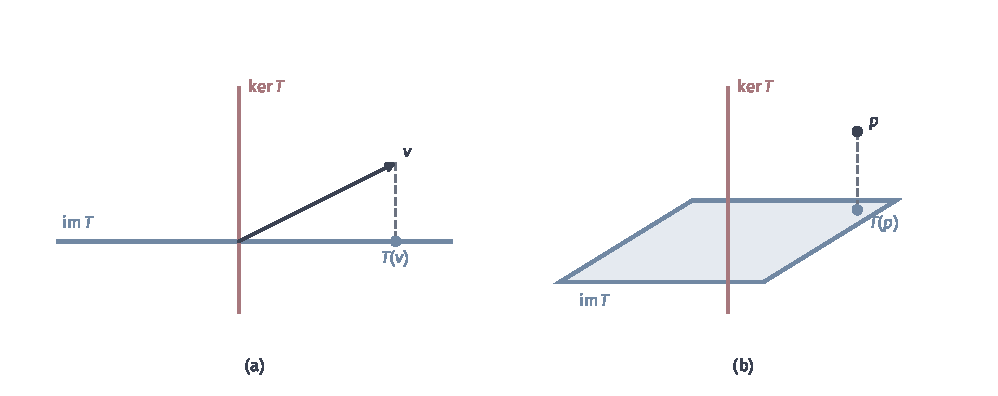
\includegraphics[width=169mm]{figures/00-shared/mathematical-preliminaries-upper/02-linear-spaces/matplotlib/ls-kernel-image-rank-nullity/ls-kernel-image-rank-nullity.pdf}
  \caption{核与像的维数此消彼长。两幅共用图面基线，红色表示核，蓝色表示像。(a)~$T(x,y)=(x,0)$把平面映到$x$轴，$\bm v=(2,1)$被映到$(2,0)$，核与像各为一维，$1+1=2$。(b)~$T(x,y,z)=(x,y)$的核是$z$轴，像是二维平面，$1+2=3$；斜投影图中$\bm p=(1,1,1)$沿虚线落到$T(\bm p)=(1,1)$。平面画在输入空间的$xy$位置，用来表示输出的两个坐标。}
  \label{fig:ls-kernel-image-rank-nullity}
\end{figure*}

秩不超过矩阵的行数和列数：$\operatorname{rank}\bm A\leq\min(m,d)$。这是因为列空间在$\mathbb R^m$中，维数不超过$m$；它又由$d$列张成，从中抽取的基不超过$d$个向量。$\operatorname{rank}\bm A=d$称为满列秩，这时输入方向全部保留，等价于各列线性无关；$\operatorname{rank}\bm A=m$称为满行秩，这时每个输出都可以到达。二者统称\term{满秩}（full rank）。

矩形矩阵不能同时满列秩和满行秩。$m<d$时，即使满行秩，核的维数也是$d-m>0$；$m>d$时，即使满列秩，像的维数也只有$d<m$，总有输出无法到达。

例如贯穿例$\bm X_\varepsilon$在$\varepsilon\neq0$时两列线性无关（示例~\ref{ex:ls-nearly-collinear-independence}），秩为$2$，满列秩；它的像是$\mathbb R^3$中的一个平面，所以不是满行秩。

\paragraph{商空间}
前面看到，输出相同的输入恰好彼此相差一个核中的向量。按输出把输入分组，每组都形如$\bm x+\ker T$，正是第~\ref{sec:ls-quotient-spaces}节取$U=\ker T$得到的等价类；全部分组组成商空间$V/\ker T$。

规则$\bm x+\ker T\mapsto T\bm x$不依赖代表元，因为代表元相差核中的向量时输出相同。它保持线性组合，并且满射到$\operatorname{im}T$。它也是单射：两个类的像相同即$T\bm x=T\bm y$时，$\bm x-\bm y\in\ker T$，两个类相同。所以它是从$V/\ker T$到$\operatorname{im}T$的线性双射。压去全部丢失的方向以后，每个等价类恰好对应一个可达输出。

线性双射把一组基送到一组基，所以两边维数相同。由式~\eqref{eq:ls-quotient-dimension}得
\[
 \dim V-\dim\ker T=\operatorname{rank}T,
\]
这是秩零度定理的另一种读法。在示例~\ref{ex:ls-kernel-indistinguishable}中，商空间$\mathbb R^4/\ker T$是三维的，像$\mathbb R^3$也是三维的。

\paragraph{证明行秩等于列秩}
现在对一般的$\bm A\in\mathbb R^{m\times d}$证明示例~\ref{ex:ls-rank-one-four-subspaces}中的维数规律。对$\bm A$用秩零度定理，零空间与列空间的维数之和为$d$；对$\bm A^\top$用秩零度定理，左零空间与行空间的维数之和为$m$。还需证明行空间与列空间的维数总相等。
\begin{theorem}[行秩等于列秩]
\label{thm:ls-row-rank-column-rank}
对任意$\bm A\in\mathbb R^{m\times d}$，$\dim\operatorname{range}(\bm A^\top)=\dim\operatorname{range}(\bm A)$，即$\operatorname{rank}\bm A^\top=\operatorname{rank}\bm A$。
\end{theorem}
\begin{proof}
设$r=\operatorname{rank}\bm A$，取列空间的一组基$\bm c_1,\ldots,\bm c_r$，排成$\bm C\in\mathbb R^{m\times r}$。$\bm A$的每一列都在列空间中，所以第$j$列可写成$\bm A_{:,j}=\bm C\bm r_j$，$\bm r_j\in\mathbb R^r$；把这些系数列排成$\bm R\in\mathbb R^{r\times d}$，按乘积的列读法得
\[
 \bm A=\bm C\bm R .
\]

再按行读这个乘积：$\bm A$的第$i$行是
\[
 \bm A_{i,:}=\sum_{k=1}^r\bm C_{i,k}\bm R_{k,:},
\]
即$\bm R$的$r$行的线性组合。所以$\bm A$的全部行都落在$\bm R$的$r$行张成的空间里，行空间的维数不超过$r$，即$\operatorname{rank}\bm A^\top\leq\operatorname{rank}\bm A$。对$\bm A^\top$用同样的论证，得$\operatorname{rank}\bm A\leq\operatorname{rank}\bm A^\top$，两者相等。
\end{proof}
于是行秩（行空间的维数）与列秩（列空间的维数）可以统称为秩。对$\bm A$与$\bm A^\top$分别用秩零度定理，四个基本子空间的维数全部由$m,d$与$r=\operatorname{rank}\bm A$决定：
\begin{equation}
 \begin{gathered}
 \dim\operatorname{range}(\bm A)=\dim\operatorname{range}(\bm A^\top)=r,\\
 \dim\operatorname{null}(\bm A)=d-r,\qquad
 \dim\operatorname{null}(\bm A^\top)=m-r.
 \end{gathered}
 \label{eq:ls-four-subspace-dimensions}
\end{equation}
输入空间中的零空间与行空间维数相加为$d$，输出空间中的列空间与左零空间维数相加为$m$。

对示例~\ref{ex:ls-rank-one-four-subspaces}中的$\bm A$，$r=1$，式~\eqref{eq:ls-four-subspace-dimensions}给出的维数与直接计算一致；证明中的分解$\bm A=\bm C\bm R$在那里就是
\[
 \bm A=(1,2)^\top(1,2,3).
\]
该示例还显示，两对子空间不仅维数互补，而且互相垂直，这要等第~\ref{sec:ls-orthogonality}节有了内积才能说清。第~\ref{sec:ls-dual-map}节还将用对偶映射给出行秩等于列秩的另一个证明。

\subsection{单射、满射与可逆性}
\phantomsection
\label{sec:ls-injective-surjective-invertible}
线性映射$T:V\to W$可逆，是说每个输出都能唯一地还原出输入。这包含两个要求：不同的输入不会给出相同的输出，称为单射；输出空间中的每个向量都能被某个输入到达，称为满射。两者都成立时称为双射，也就是可逆。对线性映射，这两个要求都可以用上一小节的核与像来检验。

\paragraph{单射与核}
单射当且仅当核为零。原因是$T\bm x=T\bm y$等价于$T(\bm x-\bm y)=\bm0$，即$\bm x-\bm y\in\ker T$。若核只含零向量，输出相同就迫使输入相同；反过来，若核中有非零向量$\bm z$，它与$\bm0$给出相同的输出$\bm0$，映射就不是单射。

\paragraph{满射与像}
满射按定义就是像等于整个输出空间。在有限维情形，两条判据都可以换成秩的条件。由秩零度定理$\dim\ker T=\dim V-\operatorname{rank}T$，核为零等价于$\operatorname{rank}T=\dim V$；像是$W$的子空间，它等于$W$当且仅当$\operatorname{rank}T=\dim W$。所以
\[
 T\text{单射}\iff\operatorname{rank}T=\dim V,\qquad
 T\text{满射}\iff\operatorname{rank}T=\dim W.
\]

\paragraph{维数与可逆性}
秩至多等于两端维数中较小的一个，所以两端维数的关系先决定了哪些性质可能成立。

若$\dim V<\dim W$，像的维数至多为$\dim V$，映射不可能满射；若$\dim V>\dim W$，核的维数至少为$\dim V-\dim W>0$，映射不可能单射。

因此，只有输入与输出维数相等的映射才可能可逆；矩形矩阵即使满秩，也只能是单射或满射之一。

维数相等时，情况反而简单。$\dim V=\dim W$时上面两个秩条件是同一个条件，单射、满射与可逆互相等价，只需检查其中任意一条，例如核是否为零。

\paragraph{方阵的可逆判据}
把这些结论用到$n$阶方阵$\bm A$上，再结合上一小节可逆映射与逆矩阵的对应，得到一串等价条件：
\[
 \bm A\text{可逆}
 \iff\operatorname{null}(\bm A)=\{\bm0\}
 \iff\operatorname{rank}\bm A=n
 \iff\bm A\text{的}n\text{列线性无关}.
\]
最后一步成立，是因为列空间由$n$列张成，维数为$n$恰好说明这$n$列构成它的一组基。由行秩等于列秩，还可以在链中加入“$\bm A$的$n$行线性无关”。

下面两个矩阵都用同一个判据检验：方阵的核是否为零。
\begin{example}[用核判断可逆]
\label{ex:ls-kernel-invertibility}
对角矩阵$\operatorname{diag}(d_1,\ldots,d_n)$逐坐标缩放，坐标之间互不影响。若每个$d_i\neq0$，逐坐标除以$d_i$即可撤销，逆矩阵为$\operatorname{diag}(1/d_1,\ldots,1/d_n)$。若某个$d_i=0$，$\bm e_i$就落入核中：两个只在第$i$个坐标上不同的输入给出相同的输出，无法还原。所以对角矩阵可逆当且仅当全部$d_i\neq0$。

矩阵
\[
 \bm A=\begin{bmatrix}2&1\\0&3\end{bmatrix}
\]
把两个坐标掺在一起，不能逐坐标撤销，但判据照样适用。$\bm A\bm x=\bm0$即
\[
 2x_1+x_2=0,\qquad 3x_2=0 .
\]
第二式给出$x_2=0$，代入第一式得$x_1=0$。核为零，所以$\bm A$可逆；按第~\ref{sec:prelim-inverse-matrices}节的二阶公式，
\[
 \bm A^{-1}=\frac16\begin{bmatrix}3&-1\\0&2\end{bmatrix}.
\]
\end{example}

这条判据不借助行列式，就能推出关于方阵的两个常用结论。

第一，方阵的单侧逆就是逆（第~\ref{sec:ls-square-one-sided-inverse}节曾用行列式证明）。若$n$阶方阵满足$\bm B\bm A=\bm I_n$，则$\bm A\bm x=\bm0$蕴含
\[
 \bm x=\bm B\bm A\bm x=\bm0,
\]
核为零，所以$\bm A$可逆，进而
\[
 \bm B=\bm B\bm A\bm A^{-1}=\bm A^{-1};
\]$\bm A\bm B=\bm I_n$时对$\bm B$作同样论证。

第二，若$n$阶方阵的乘积$\bm A\bm B$可逆，则两个因子都可逆。$\bm B\bm x=\bm0$蕴含$\bm A\bm B\bm x=\bm0$，从而$\bm x=\bm0$，所以$\bm B$的核为零、$\bm B$可逆；于是$\bm A=(\bm A\bm B)\bm B^{-1}$是两个可逆矩阵的乘积，也可逆。

\paragraph{单侧逆}
维数不同时不能完全撤销，但可以从一侧撤销。若$T:V\to W$是单射，存在线性映射$L:W\to V$使$L\circ T=\operatorname{id}_V$：在像上按$T$的逆读回输入，在像的一个补空间上任意规定，例如全部送到零。若$T$是满射，存在线性映射$R:W\to V$使$T\circ R=\operatorname{id}_W$：为输出基中的每个向量任选一个原像，再线性延拓。补空间与原像都有多种选法，所以这些单侧逆一般不唯一。

写成矩阵，对$\bm A\in\mathbb R^{m\times d}$：$\bm A$有左逆当且仅当它满列秩，有右逆当且仅当它满行秩。充分性来自上面的构造，因为满列秩就是单射，满行秩就是满射。必要性同样直接：若$\bm L\bm A=\bm I_d$，则$\bm A\bm x=\bm0$蕴含$\bm x=\bm L\bm A\bm x=\bm0$，核为零；若$\bm A\bm R=\bm I_m$，则每个$\bm y=\bm A(\bm R\bm y)$都能到达。

\subsection{换基与相抵}
\label{sec:ls-coordinates-change-of-basis}
\phantomsection
\label{sec:ls-equivalence-matrices}

第~\ref{sec:ls-coordinates}节看到，同一个向量在不同的基下有不同的坐标。线性映射也是这样：映射本身不变，换一组基，记录它的矩阵通常就会改变。这一小节和下一小节写出这种变化的规律，并回答一个反方向的问题：给定两个矩阵，怎样判断它们记录的是不是同一个映射。

需要区分两种情形。一般的线性映射$T:V\to W$两端是两个空间，可以各自换基，由此得到的矩阵关系称为相抵，是本小节的内容。线性算子$T:V\to V$两端是同一个空间，换基时两端必须一起换，由此得到的关系称为相似，留到下一小节。相似多了“两端换基相同”这一约束，可调整的余地更小：后面会看到，相抵只用秩就能完全分类，相似则需要更多不变量。

推导时要用到一个观察：换基矩阵本身就是一个线性映射的矩阵。比较式~\eqref{eq:linear-algebra-coordinate-change}与式~\eqref{eq:linear-algebra-map-matrix-representation}可见，$\bm S_{\mathcal C\leftarrow\mathcal B}$正是恒等映射$\operatorname{id}_V$以$\mathcal B$为输入基、$\mathcal C$为输出基的矩阵：向量不动，只是两端用不同的基记录。连续换基时换基矩阵相乘，就是复合公式~\eqref{eq:ls-composition-matrix}用于$\operatorname{id}_V\circ\operatorname{id}_V=\operatorname{id}_V$的特例。

下面设$T:V\to W$是线性映射，$\dim V=d$、$\dim W=m$。先求出$T$在两对基下的矩阵之间的关系，再说明这一关系恰好刻画“记录同一个映射”，最后证明只需比较秩就能判断。

\subsubsection{相抵的定义}
\label{sec:ls-equivalence-definition}
先从换基推导两种记录之间的关系，再据此给出定义。

设$\mathcal B,\mathcal B'$是$V$的旧基与新基，$\mathcal C,\mathcal C'$是$W$的旧基与新基，$T$在旧基下的矩阵为$\bm A=[T]_{\mathcal C\leftarrow\mathcal B}$，在新基下的矩阵为$\bm B=[T]_{\mathcal C'\leftarrow\mathcal B'}$。两端的换基矩阵记为
\[
 \bm P=\bm S_{\mathcal B\leftarrow\mathcal B'}\ (d\text{阶可逆}),\qquad
 \bm Q=\bm S_{\mathcal C\leftarrow\mathcal C'}\ (m\text{阶可逆}),
\]
$\bm P$的第$j$列是第$j$个新输入基向量在旧输入基下的坐标，$\bm Q$同理。

要从新输入坐标$[\bm v]_{\mathcal B'}$求出新输出坐标$[T\bm v]_{\mathcal C'}$，可以绕道旧基走三步。先把新输入坐标换成旧输入坐标，再在旧基下作用：
\[
 [\bm v]_{\mathcal B}=\bm P[\bm v]_{\mathcal B'},\qquad
 [T\bm v]_{\mathcal C}=\bm A[\bm v]_{\mathcal B}.
\]
最后用反向换基矩阵$\bm Q^{-1}=\bm S_{\mathcal C'\leftarrow\mathcal C}$把旧输出坐标换成新输出坐标。合起来是
\[
 [T\bm v]_{\mathcal C'}=\bm Q^{-1}[T\bm v]_{\mathcal C}=\bm Q^{-1}\bm A\bm P[\bm v]_{\mathcal B'}.
\]

另一方面，按定义
\[
 [T\bm v]_{\mathcal C'}=\bm B[\bm v]_{\mathcal B'} .
\]
两式对每个$\bm v$都成立。取$\bm v$为第$j$个新输入基向量，它的新坐标是$\bm e_j$，两边读出的就是两个矩阵的第$j$列。所以
\begin{equation}
 \bm B=\bm Q^{-1}\bm A\bm P.
 \label{eq:ls-equivalence-transform}
\end{equation}
从右向左读，$\bm P$把新输入坐标换成旧坐标，$\bm A$在旧基下作用，$\bm Q^{-1}$把结果换成新输出坐标。也可以用复合来理解：$T=\operatorname{id}_W\circ T\circ\operatorname{id}_V$，三个因子各自在相应的基下记录，由式~\eqref{eq:ls-composition-matrix}就得到右端的三个矩阵。

\phantomsection
\label{sec:ls-equivalence-meaning}%
上面的推导表明，同一个映射的两种记录之间，只差在两侧各乘一个可逆矩阵。把这种关系单独命名。
\begin{definition}[矩阵相抵]
\label{def:ls-matrix-equivalence}
设$\bm A,\bm B\in\mathbb R^{m\times d}$。若存在可逆矩阵$\bm Q\in\mathbb R^{m\times m}$与$\bm P\in\mathbb R^{d\times d}$使$\bm B=\bm Q^{-1}\bm A\bm P$，就称$\bm A$与$\bm B$\term{相抵}（equivalent matrices）。
\end{definition}
定义中的$\bm Q,\bm P$可以是任意可逆矩阵，不必事先知道它们来自哪组基。写成$\bm Q^{-1}$只是为了与换基推导一致；$\bm Q$取遍全部可逆矩阵时，$\bm Q^{-1}$也取遍全部可逆矩阵。

反过来，任意一对可逆矩阵都对应一次换基，所以相抵恰好刻画“记录同一个映射”。设$\bm A=[T]_{\mathcal C\leftarrow\mathcal B}$，任给可逆的$\bm P,\bm Q$。由第~\ref{sec:ls-coordinates}节，以$\bm P$的各列为旧基下的坐标，可以构造$V$的一组新基$\mathcal B'$，使$\bm S_{\mathcal B\leftarrow\mathcal B'}=\bm P$；输出端用$\bm Q$同样构造$\mathcal C'$。按换基过程，$T$在这两组新基下的矩阵正是$\bm Q^{-1}\bm A\bm P$。因此，两个同形矩阵相抵，当且仅当它们是同一个线性映射在两端不同选基下的记录。

在这个意义下，右乘$\bm P$对应更换输入基，左乘$\bm Q^{-1}$对应更换输出基。初等列变换与初等行变换就是这两种换基最简单的具体形式。

\subsubsection{相抵的性质}
\label{sec:ls-equivalence-properties}
相抵的矩阵记录同一个映射，映射本身的性质就不应随基改变。下面逐条给出相抵的性质。

首先，“相抵”可以像“相等”一样使用：它是等价关系。
\begin{theorem}[相抵是等价关系]
\label{thm:ls-equivalence-relation}
在$\mathbb R^{m\times d}$上：每个矩阵与自身相抵；若$\bm A$与$\bm B$相抵，则$\bm B$与$\bm A$相抵；若$\bm A$与$\bm B$相抵、$\bm B$与$\bm C$相抵，则$\bm A$与$\bm C$相抵。
\end{theorem}
\begin{proof}
自反性取$\bm Q=\bm P=\bm I$。

对称性：由$\bm B=\bm Q^{-1}\bm A\bm P$得$\bm A=\bm Q\bm B\bm P^{-1}=(\bm Q^{-1})^{-1}\bm B\bm P^{-1}$。

传递性：若$\bm B=\bm Q_1^{-1}\bm A\bm P_1$、$\bm C=\bm Q_2^{-1}\bm B\bm P_2$，则$\bm C=(\bm Q_1\bm Q_2)^{-1}\bm A(\bm P_1\bm P_2)$。

三条分别对应不换基、换回原基和连续换两次基。
\end{proof}

其次，换基只是把零空间和列空间“搬”到新的坐标下，并不改变它们。
\begin{theorem}[相抵下的零空间与列空间]
\label{thm:ls-equivalence-subspaces}
若$\bm B=\bm Q^{-1}\bm A\bm P$，其中$\bm Q,\bm P$可逆，则
\[
 \operatorname{null}(\bm B)=\bm P^{-1}\operatorname{null}(\bm A),\qquad
 \operatorname{range}(\bm B)=\bm Q^{-1}\operatorname{range}(\bm A).
\]
\end{theorem}
\begin{proof}
$\bm B\bm x=\bm0$当且仅当$\bm A(\bm P\bm x)=\bm0$，即$\bm P\bm x\in\operatorname{null}(\bm A)$，所以零空间在输入端被$\bm P^{-1}$搬运。又$\bm B\bm x=\bm Q^{-1}\bm A(\bm P\bm x)$，而$\bm x$取遍全部输入时$\bm P\bm x$也取遍全部输入，所以列空间在输出端被$\bm Q^{-1}$搬运。
\end{proof}

最后，可逆矩阵把线性无关组送到线性无关组，因而不改变子空间的维数。由上一定理立即得到最常用的不变量。
\begin{theorem}[相抵保持秩]
\label{thm:ls-equivalence-invariants}
相抵的矩阵$\bm A,\bm B\in\mathbb R^{m\times d}$秩相同，零空间维数也相同：
\begin{equation}
\begin{gathered}
\operatorname{rank}\bm B=\operatorname{rank}\bm A\\
\dim\operatorname{null}(\bm B)=\dim\operatorname{null}(\bm A)=d-\operatorname{rank}\bm A.
\end{gathered}
\label{eq:ls-equivalence-invariants}
\end{equation}
\end{theorem}
\begin{proof}
由定理~\ref{thm:ls-equivalence-subspaces}，$\operatorname{range}(\bm B)$与$\operatorname{null}(\bm B)$分别是$\operatorname{range}(\bm A)$与$\operatorname{null}(\bm A)$在可逆矩阵下的像，维数不变；第二个等式的右端由秩零度定理给出。
\end{proof}

幂、迹这类量不在相抵的讨论之列：相抵允许输入与输出是不同的空间，$\bm B$一般不是方阵，不能对自身反复作用。

\subsubsection{相抵的判据}
\label{sec:ls-equivalence-conditions}
秩在相抵下不变；反过来，秩相同的两个同形矩阵也一定相抵。证明的思路是：两端可以各自选基时，每个矩阵都能化成只由秩决定的简单形状。

设$\bm A$是$T$在某对基下的矩阵，$r=\operatorname{rank}\bm A$。在输入端，取$\ker T$的一组基，再扩充为$V$的一组基；由秩零度定理，新增的向量恰有$r$个，把它们排在前面。这$r$个向量的像线性无关：若像的某个组合为零，相应的新增向量组合就落进核里，能由核的基表示，而整组基线性无关，迫使系数全为零。核的基向量的像都是零，所以这$r$个像还张成$\operatorname{im}T$。

在输出端，把这$r$个像扩充为$W$的一组基。在这样选取的两组基下，$T$把前$r$个输入基向量依次送到前$r$个输出基向量，把其余输入基向量送到零，矩阵为秩标准形
\begin{equation}
 \begin{bmatrix}\bm I_r&\bm0\\\bm0&\bm0\end{bmatrix},\qquad r=\operatorname{rank}\bm A.
\label{eq:ls-rank-normal-form}
\end{equation}

下面对一个秩为$1$的二阶矩阵具体做出这两组基。
\begin{example}[两端各自选基化为秩标准形]
\label{ex:ls-rank-normal-form-two-by-two}
设$T\bm x=\bm A\bm x$，其中
\[
 \bm A=\begin{bmatrix}1&2\\2&4\end{bmatrix},
\]
两端原来都用标准基。两列共线，$\operatorname{rank}\bm A=1$；又$\bm A(-2,1)^\top=\bm0$，所以$\ker T=\operatorname{span}\{(-2,1)^\top\}$。

按上面的构造选基。输入端把核的基向量$\bm v_2=(-2,1)^{\top}$放在后面，前面补一个不在核中的$\bm v_1=\bm e_1$；输出端先取它的像$\bm w_1=\bm A\bm v_1=(1,2)^{\top}$，再补上$\bm w_2=\bm e_2$凑成一组基。以新基向量的标准坐标为列，得到两端的换基矩阵
\[
 \bm P=\begin{bmatrix}1&-2\\0&1\end{bmatrix},\qquad
 \bm Q=\begin{bmatrix}1&0\\2&1\end{bmatrix}.
\]
输出端的换基矩阵还要求逆，得
\[
 \bm Q^{-1}=\begin{bmatrix}1&0\\-2&1\end{bmatrix}.
\]
先算$\bm A\bm P$，它的两列就是$\bm v_1,\bm v_2$的像的标准坐标：
\[
 \bm A\bm P=\begin{bmatrix}1&0\\2&0\end{bmatrix}.
\]
再左乘$\bm Q^{-1}$，把这两个像改用输出基$\bm w_1,\bm w_2$记录：
\[
 \bm Q^{-1}\bm A\bm P=\begin{bmatrix}1&0\\-2&1\end{bmatrix}\begin{bmatrix}1&0\\2&0\end{bmatrix}
 =\begin{bmatrix}1&0\\0&0\end{bmatrix}.
\]
结果正是秩标准形$\operatorname{diag}(1,0)$：在新基下，$T$把$\bm v_1$送到$\bm w_1$，把核方向$\bm v_2$送到零。
\end{example}
图~\ref{fig:ls-equivalence-two-sided-bases-flow}画出这两组基：$\bm v_1$被送到$\bm w_1$，核方向$\bm v_2$被送到零，输出端的$\bm w_2$不被任何输入到达。这几点要同时做到，需要两端各自选基；若要求两端用同一组基，这样的化简一般做不到。
\begin{figure}[!htb]
  \centering
  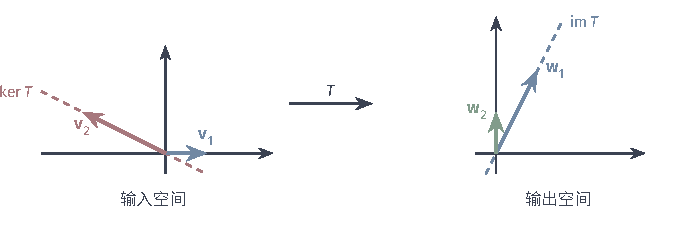
\includegraphics[width=112mm]{figures/00-shared/mathematical-preliminaries-upper/02-linear-spaces/tikz/comprehension-additions/equivalence-two-bases.pdf}
  \caption{两端各自选基化为秩标准形。$T(\bm x)=\bm A\bm x$，$\bm A=\left[\begin{smallmatrix}1&2\\2&4\end{smallmatrix}\right]$。左：输入基$\bm v_1=\bm e_1$（蓝）与$\bm v_2=(-2,1)^{\top}$（红），$\bm v_2$在核（红虚线）上。右：输出基$\bm w_1=T\bm v_1=(1,2)^{\top}$（蓝）位于像（蓝虚线）上，$\bm w_2=\bm e_2$（绿）补足一组基。在这两组基下$T$的矩阵为$\operatorname{diag}(1,0)$。}
  \label{fig:ls-equivalence-two-sided-bases-flow}
\end{figure}

有了秩标准形，就得到相抵的完整判据。
\begin{theorem}[相抵判据]
\label{thm:ls-equivalence-criterion}
两个同形实矩阵$\bm A,\bm B\in\mathbb R^{m\times d}$相抵，当且仅当$\operatorname{rank}\bm A=\operatorname{rank}\bm B$。
\end{theorem}
\begin{proof}
必要性由定理~\ref{thm:ls-equivalence-invariants}得到。充分性：设二者秩都为$r$，由上面的构造，存在可逆矩阵使
\[
 \bm R=\bm Q_A^{-1}\bm A\bm P_A=\bm Q_B^{-1}\bm B\bm P_B,
\]
其中$\bm R$是式\eqref{eq:ls-rank-normal-form}的秩标准形。两式对接得
\[
 \bm B=(\bm Q_A\bm Q_B^{-1})^{-1}\bm A(\bm P_A\bm P_B^{-1}),
\]
即二者相抵。
\end{proof}
所以形状固定以后，秩就是判断相抵的唯一依据：零矩阵只与零矩阵相抵，同形的满秩矩阵彼此相抵。

实际把矩阵化到秩标准形，可以交替使用第~\ref{sec:ls-elementary-row-operations}节的初等行变换与相应的初等列变换；数值计算中的消元算法在第~\ref{chap:direct-linear-solvers}章建立。

\subsection{换基与相似}
\label{sec:ls-similarity}
\phantomsection
\label{sec:ls-matrix-equivalences}

线性算子$T:V\to V$的输入与输出是同一个空间。记录它时两端用同一组基，换基时两端也要换成同一组新基。本小节把这一约束加进上一小节的推导，得到相似关系，再讨论相似保持哪些量，以及怎样判断两个方阵是否相似。

\subsubsection{相似的定义}
\label{sec:ls-similarity-definition}
设$\mathcal B$与$\mathcal B'$是$V$的旧基与新基，$\bm A=[T]_{\mathcal B}$、$\bm B=[T]_{\mathcal B'}$，换基矩阵$\bm P=\bm S_{\mathcal B\leftarrow\mathcal B'}$的第$j$列是第$j$个新基向量在旧基下的坐标。

两端是同一个空间、同一次换基，所以上一小节三步推导中的$\bm Q$就是$\bm P$。先把新坐标换成旧坐标，再在旧基下作用：
\[
 [\bm v]_{\mathcal B}=\bm P[\bm v]_{\mathcal B'},\qquad
 [T\bm v]_{\mathcal B}=\bm A\bm P[\bm v]_{\mathcal B'}.
\]
再把输出换回新坐标，
\[
 [T\bm v]_{\mathcal B'}=\bm P^{-1}[T\bm v]_{\mathcal B}=\bm P^{-1}\bm A\bm P[\bm v]_{\mathcal B'}.
\]
与$[T\bm v]_{\mathcal B'}=\bm B[\bm v]_{\mathcal B'}$逐列比较，得到
\begin{equation}
 \bm B=\bm P^{-1}\bm A\bm P.
 \label{eq:linear-algebra-similarity-change-basis}
\end{equation}
它就是式~\eqref{eq:ls-equivalence-transform}取$\bm Q=\bm P$的情形。

\phantomsection
\label{sec:ls-similarity-meaning}%
与相抵一样，给同一算子两种记录之间的关系单独命名。
\begin{definition}[矩阵相似]
\label{def:ls-matrix-similarity}
设$\bm A,\bm B$是$n$阶方阵。若存在$n$阶可逆矩阵$\bm P$使$\bm B=\bm P^{-1}\bm A\bm P$，就称$\bm A$与$\bm B$\term{相似}（similar）。
\end{definition}
和相抵的论证相同，任意可逆的$\bm P$都对应一次换基：给定$\bm A=[T]_{\mathcal B}$，以$\bm P$的各列为旧基下的坐标构造新基，$T$在新基下的矩阵恰为$\bm P^{-1}\bm A\bm P$。所以两个方阵相似，当且仅当它们是同一个线性算子在两组基下的记录。

注意相似并不要求$\bm A,\bm B$本身可逆，要求可逆的只是换基矩阵$\bm P$。取$\bm Q=\bm P$可见，相似的矩阵一定相抵；反之不然，后面的示例~\ref{ex:ls-equivalent-not-similar}给出秩相同、因而相抵，却不相似的两个矩阵。

换基的一个用处是简化算子的矩阵。下面的例子把一个上三角矩阵化成对角形。
\begin{example}[换基把算子的矩阵化为对角形]
\label{ex:ls-similarity-diagonal}
示例~\ref{ex:ls-plane-operator-matrix}中的算子$T(x_1,x_2)=(2x_1+x_2,3x_2)$在标准基下的矩阵为
\[
 \bm A=\begin{bmatrix}2&1\\0&3\end{bmatrix},
\]
即$T\bm e_1=2\bm e_1$、$T\bm e_2=\bm e_1+3\bm e_2$。$\bm e_1$只被伸长，$\bm e_2$的像却混入了$\bm e_1$方向，这就是非对角元$1$的来源。改取新基$\bm b_1'=\bm e_1$、$\bm b_2'=\bm e_1+\bm e_2$，换基矩阵以新基向量的标准坐标为列，它和它的逆为
\[
 \bm P=\begin{bmatrix}1&1\\0&1\end{bmatrix},\quad
 \bm P^{-1}=\begin{bmatrix}1&-1\\0&1\end{bmatrix},
\]
于是
\[
 \bm B=\bm P^{-1}\bm A\bm P
 =\begin{bmatrix}1&-1\\0&1\end{bmatrix}
 \begin{bmatrix}2&1\\0&3\end{bmatrix}
 \begin{bmatrix}1&1\\0&1\end{bmatrix}.
\]
依次相乘，得
\[
 \bm B=\begin{bmatrix}2&0\\0&3\end{bmatrix}.
\]

不经矩阵乘法也能看出这一结果：$T\bm b_1'=2\bm b_1'$，而
\[
 T\bm b_2'=T\bm e_1+T\bm e_2=3\bm e_1+3\bm e_2=3\bm b_2'.
\]
两个新基方向在$T$的作用下都只被伸缩、不被转向，彼此互不干扰，所以$T$在新基下的矩阵是对角矩阵$\operatorname{diag}(2,3)$。
\end{example}
$T$本身没有改变，改变的只是沿哪两个方向读取它的作用。图~\ref{fig:ls-similarity-change-of-basis-flow}把这一点画在平面上。在标准基下，单位正方形被$T$拉成一个斜的平行四边形，所以矩阵$\bm A$有非零的非对角元；在新基下，基向量围成的平行四边形只沿两个基方向分别伸长$2$倍和$3$倍，所以矩阵是对角的$\bm B$。

\begin{figure}[!htb]
  \centering
  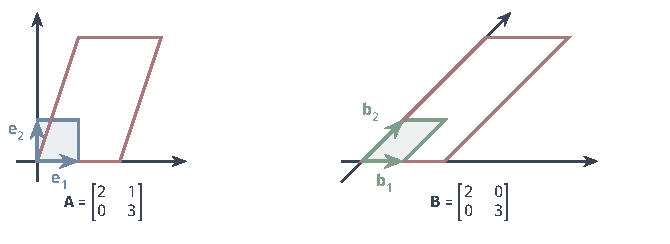
\includegraphics[width=112mm]{figures/00-shared/mathematical-preliminaries-upper/02-linear-spaces/tikz/comprehension-additions/similarity-two-bases.pdf}
  \caption{同一个算子在两组基下的记录。左：标准基$\bm e_1,\bm e_2$围成的单位正方形（蓝）被$\bm A=\left[\begin{smallmatrix}2&1\\0&3\end{smallmatrix}\right]$送到红色平行四边形，形状被斜切。右：新基$\bm b_1=\bm e_1$、$\bm b_2=\bm e_1+\bm e_2$围成的平行四边形（绿）被同一个算子送到红色平行四边形，只沿$\bm b_1$伸长$2$倍、沿$\bm b_2$伸长$3$倍，因此新矩阵为$\operatorname{diag}(2,3)$。}
  \label{fig:ls-similarity-change-of-basis-flow}
\end{figure}

\subsubsection{相似的性质}
\label{sec:ls-similarity-properties}
同一个算子的性质不随基改变。相似是相抵的特例，相抵的不变量自然保持；算子还能对自身反复作用，由此得到更多不变量。下面逐条给出。以下设$\bm A,\bm B$是$n$阶方阵，$\bm B=\bm P^{-1}\bm A\bm P$，$\bm P$可逆。
\begin{theorem}[相似是等价关系]
\label{thm:ls-similarity-relation}
在$n$阶方阵上：每个矩阵与自身相似；若$\bm A$与$\bm B$相似，则$\bm B$与$\bm A$相似；若$\bm A$与$\bm B$相似、$\bm B$与$\bm C$相似，则$\bm A$与$\bm C$相似。
\end{theorem}
\begin{proof}
自反性：$\bm A=\bm I^{-1}\bm A\bm I$。对称性：$\bm A=\bm P\bm B\bm P^{-1}=(\bm P^{-1})^{-1}\bm B\bm P^{-1}$。传递性：若再有$\bm C=\bm R^{-1}\bm B\bm R$，则$\bm C=(\bm P\bm R)^{-1}\bm A(\bm P\bm R)$。
\end{proof}

\begin{theorem}[相似保持秩]
\label{thm:ls-similarity-invariants}
相似的矩阵秩相同，零空间维数也相同：
\begin{equation}
\begin{gathered}
\operatorname{rank}\bm B=\operatorname{rank}\bm A\\
\dim\operatorname{null}(\bm B)=\dim\operatorname{null}(\bm A).
\end{gathered}
\label{eq:ls-similarity-invariants}
\end{equation}
\end{theorem}
\begin{proof}
取$\bm Q=\bm P$，相似的矩阵相抵，由定理~\ref{thm:ls-equivalence-invariants}即得。
\end{proof}

算子可以对自身反复作用，而反复作用与换基相容。
\begin{theorem}[乘积与幂的换基]
\label{thm:ls-similarity-powers}
若还有$\bm B_2=\bm P^{-1}\bm A_2\bm P$，则
\begin{equation}
 \bm B\bm B_2=\bm P^{-1}\bm A\bm A_2\bm P.
 \label{eq:ls-similarity-product}
\end{equation}
特别地，对每个正整数$k$，
\[
 \bm B^k=\bm P^{-1}\bm A^k\bm P.
\]
\end{theorem}
\begin{proof}
把两个换基式相乘，
\[
 \bm B\bm B_2=\bm P^{-1}\bm A\bm P\,\bm P^{-1}\bm A_2\bm P=\bm P^{-1}\bm A\bm A_2\bm P,
\]
中间的$\bm P\bm P^{-1}$相消；对$k$归纳即得幂的公式。
\end{proof}
换基以后，反复作用记录的仍是同一个过程。

把单位矩阵的倍数减掉，相似关系仍然保持，由此得到比秩更细的一族不变量。
\begin{theorem}[移位后的秩]
\label{thm:ls-similarity-shifted-rank}
对每个实数$c$，$\bm B-c\bm I$与$\bm A-c\bm I$相似，因而
\begin{equation}
\operatorname{rank}(\bm B-c\bm I)=\operatorname{rank}(\bm A-c\bm I),\qquad c\in\mathbb R.
\label{eq:ls-similarity-shifted-rank}
\end{equation}
\end{theorem}
\begin{proof}
把$c\bm I$写成$c\bm P^{-1}\bm P$，得
\[
 \bm B-c\bm I=\bm P^{-1}\bm A\bm P-c\bm P^{-1}\bm P=\bm P^{-1}(\bm A-c\bm I)\bm P,
\]
再由定理~\ref{thm:ls-similarity-invariants}。
\end{proof}
每个$c$都给出一个不变量；$c=0$时就是秩本身。

最后，相似保持两个可以直接计算的标量。
\begin{theorem}[行列式与迹不变]
\label{thm:ls-similarity-det-trace}
$\det\bm B=\det\bm A$，$\operatorname{tr}\bm B=\operatorname{tr}\bm A$。
\end{theorem}
\begin{proof}
由行列式的乘法性（第~\ref{sec:ls-determinant-properties}节）与$\det(\bm P^{-1})\det\bm P=\det\bm I=1$，
\[
 \det(\bm P^{-1}\bm A\bm P)=\det(\bm P^{-1})\,\det\bm A\,\det\bm P=\det\bm A;
\]
由迹的循环性（式~\eqref{eq:linear-algebra-trace-cyclic}），
\[
 \operatorname{tr}(\bm P^{-1}\bm A\bm P)=\operatorname{tr}\bigl((\bm A\bm P)\bm P^{-1}\bigr)=\operatorname{tr}\bm A.
\]
\end{proof}
所以行列式与迹只依赖算子本身，可以说“算子$T$的行列式”“算子$T$的迹”，用任意一组基下的矩阵计算即可。例如示例~\ref{ex:ls-similarity-diagonal}中的$\bm A$与$\bm B=\operatorname{diag}(2,3)$，行列式都是$6$，迹都是$5$。

引入特征值以后还将看到（第~\ref{sec:ls-eigen-similarity-invariance}节），特征值与特征多项式同样是相似不变量，而行列式与迹恰好是特征值之积与特征值之和。一般的换基不保持欧氏长度与夹角，这些度量量不是相似不变量。

\subsubsection{相似的判据}
\label{sec:ls-similarity-conditions}
判断两个给定的方阵是否相似，可以把定义改写成线性方程。两端左乘$\bm P$，相似就是存在\emph{可逆}的$\bm P$满足
\begin{equation}
 \bm A\bm P=\bm P\bm B.
 \label{eq:ls-similarity-equation}
\end{equation}
这是关于$\bm P$各元素的一组线性方程。注意解必须可逆：非零但不可逆的解只把一部分方向对应起来，不构成两组基之间的换基。

不变量给出否定的判据：只要某个相似不变量不同，两个矩阵就不相似。反过来却不成立。秩、行列式、迹相同都只是相似的必要条件，下面的例子说明它们合在一起也不充分。
\begin{example}[反例：相抵而不相似的两个矩阵]
\label{ex:ls-equivalent-not-similar}
比较$\bm I_2$与
\[
 \bm J=\begin{bmatrix}1&1\\0&1\end{bmatrix}.
\]
前面列出的不变量都分不开它们：二者都可逆，秩都为$2$，由相抵判据它们相抵；行列式都是$1$，迹都是$2$。移位后的秩却不同。取$c=1$，$\bm I_2-\bm I_2=\bm0$的秩为$0$，而
\[
 \bm J-\bm I_2=\begin{bmatrix}0&1\\0&0\end{bmatrix}
\]
的秩为$1$，式~\eqref{eq:ls-similarity-shifted-rank}不成立，所以二者不相似。

这个结论也可以直接看出：若$\bm J=\bm P^{-1}\bm I_2\bm P$，则$\bm J=\bm P^{-1}\bm P=\bm I_2$，矛盾。单位矩阵在任何基下都是单位矩阵，只与自己相似；$\bm J$与它相抵，秩、行列式与迹也都相同，却不是同一个算子的记录。
\end{example}
这正是“两端换基相同”这一约束的代价：判断相抵时秩相同就足够，判断相似时秩、行列式与迹一起相同都不够。比较$\bm A-c\bm I$在各个$c$处的秩是更细的必要条件；完整的相似分类需要Jordan标准形，本书不展开。

\subsection{多线性映射}
\label{sec:ls-multilinear-maps}

前面的线性映射只有一个输入。矩阵的元素内积、两个向量的外积都有两个输入：固定其中一个、改变另一个时，结果保持线性组合。描述这种逐个输入的线性，要为每个输入保留一个独立的位置，称为槽位。

设$V_1,\ldots,V_k,W$是同一数域上的线性空间。若映射$F:V_1\times\cdots\times V_k\to W$在固定其余输入后，对每一个输入都是线性的，就称为多线性映射；$k=2$时称为双线性映射。例如$F(\bm x,\bm y)=\bm x\bm y^\top$对两个输入分别线性。

对每个输入分别线性，不等于把输入组看成一个整体后线性。以实数乘法$f(x,y)=xy$为例，$f(1,1)+f(1,1)=2$，但$f(2,2)=4$。

选定各输入空间的基后，多线性映射也能由有限组系数记录。以实双线性函数$B:V\times W\to\mathbb R$为例，取基$(\bm v_i)$与$(\bm w_j)$，令$b_{i,j}=B(\bm v_i,\bm w_j)$。当$\bm x=\sum_i x_i\bm v_i$、$\bm y=\sum_j y_j\bm w_j$时，逐个槽位展开得到
\[
 B(\bm x,\bm y)=\sum_{i,j}x_i y_j b_{i,j}.
\]
因此，基向量两两配对的值足以确定任意输入下的值。换基会改变这些系数，映射本身不变。这组系数就是第~\ref{sec:ls-tensor-products}节张量积与指标缩约所用的系数数组：上式右端正是系数表$(b_{i,j})$与两列坐标的张量积$[\bm x]\otimes[\bm y]$的Frobenius配对。不过，重排数组的存放次序只改变存放方式，不等于更换坐标基；换基改变的是系数表本身的数值。

\section{本章小结}
\label{sec:ls-representation-summary}

本章把对象与记录对象的数分开。线性空间规定哪些对象可以相加和缩放，子空间是其中对线性组合封闭的部分。子空间可以求交、求和；交为零时和是直和，分解唯一。商空间则把相差某个子空间中向量的对象视为相同。

基同时满足张成与线性无关，所以每个向量有唯一的坐标。基的向量个数与选取无关，这个数就是维数；“先取已有的基，再补新方向”给出和空间、补空间与商空间的维数。换基改变坐标，不改变向量，新旧坐标由可逆的换基矩阵换算。基接近退化时，坐标可能很大，不能用来判断对象的大小。

线性映射保持线性组合。选定两端的基，它记成矩阵，叠加、复合与求逆分别对应矩阵的加法、乘法与求逆。核记录丢失的输入，像记录能到达的输出，秩零度定理说明二者的维数之和等于输入维数；由此可以判断单射、满射与可逆。同一个映射在不同基下的矩阵相差两侧的可逆因子：两端各自换基得到相抵，秩是它的完整不变量；算子两端同时换基得到相似，秩、行列式与迹相同仍不足以保证相似。

回到章首的问题：坐标和矩阵都是在选定基以后才有的记录，换基时它们按可逆矩阵换算；张成、线性无关、维数、核与像的维数、秩、相似矩阵的行列式与迹，则是对象或映射本身的性质，不随记录方式改变。这些结构还没有规定向量的大小或夹角，所以近共线基下的大坐标究竟意味着什么，还无法定量回答。第~\ref{chap:normed-spaces}章引入范数，讨论大小与收敛；第~\ref{chap:inner-product-spaces}章引入内积，讨论正交分解与最佳近似；第~\ref{chap:dual-spaces}章再研究把向量读成一个数的线性泛函。


\chapter{赋范空间}
\label{chap:normed-spaces}
\label{chap:normed-inner-product-spaces}

上一章的线性空间只有加法和数乘。借助它们可以判断一个向量能否由给定向量线性表示、表示是否唯一，却无法回答两个向量相差多少、一列近似是否趋于某个极限。本章用范数给线性空间规定大小，回答这两个问题；角度与正交留给第~\ref{chap:inner-product-spaces}章的内积。

第~\ref{sec:ls-normed-spaces}节给出范数的公理与例子，说明第~\ref{chap:linear-operations}章的坐标范数满足这些公理，并证明有限维空间中任意两个范数等价，所以后面的概念都可以在任意范数下定义，并且不依赖所选范数。

在此基础上，第~\ref{sec:multivariable-open-closed-sets}节定义开集、闭集与有界集；第~\ref{sec:multivariable-limits-continuity}节定义序列的收敛，证明有限维空间完备、有界序列有收敛子列、子空间都是闭集，再讨论级数的极限与映射的联合极限；第~\ref{sec:multivariable-continuity}节研究连续性，证明闭有界集上的连续函数取到最值、一致连续。第~\ref{sec:ls-derived-norms}节再定义两种导出的范数：矩阵范数衡量线性映射的最大放大倍数，商范数衡量忽略一个子空间后剩下的大小。第~\ref{chap:linear-recurrence-stability}章的矩阵幂与Neumann级数、第~\ref{chap:stationary-iterations}章的迭代以及第~\ref{chap:multivariate-differentiation}章的微分，都使用这套分析基础。

本章依赖前两章的线性运算、基与坐标，以及一元分析中的数列极限、确界和最值定理（第~\ref{sec:multivariable-limits-continuity}节开头说明所用的结论）。全章只讨论有限维空间；收敛与连续性适用于一般映射，不限于线性映射。无限维的函数空间中，范数等价、完备性和最近点存在都可能失败，那里的理论可参考\BookChapterRef{chap:functional-analysis-and-approximation}{卷四“函数空间”一章}。

% 赋范空间：范数与距离；收敛、极限与连续性；有限维赋范空间的性质（范数等价、完备性、级数、矩阵范数、对偶范数、商范数），只讨论有限维情形。

\section{范数与距离}
\label{sec:ls-normed-spaces}

用多项式近似一个函数时，要估计误差有多大；迭代产生一列近似时，要判断它是否趋于某个对象。这些问题都需要先规定向量的大小。第~\ref{chap:linear-operations}章用$\ell_1$、$\ell_2$、$\ell_\infty$范数度量$\mathbb R^d$中数组的大小，本节把这种度量推广到一般线性空间。

本节先给出范数的公理和例子，这一部分只用到线性运算与标量不等式；坐标范数之间的比较已在第~\ref{sec:ls-error-scale-comparison}节给出。然后证明有限维空间中任意两个范数等价，此后的开集、闭集、收敛、极限与连续性因而都不依赖所选范数；第~\ref{sec:ls-derived-norms}节再在矩阵、线性泛函和商空间上定义范数。本章只讨论有限维空间。

\subsection{范数的定义与示例}
\label{sec:ls-normed-space-definition}

\paragraph{范数的定义}
第~\ref{sec:ls-p-norm-properties}节证明了，$p$范数非负、正定、齐次，并满足三角不等式。这些性质只涉及加法和数乘，因此可以直接作为一般线性空间上“大小”的要求。
\begin{definition}[赋范空间]
\label{def:ls-normed-space}
\label{def:functional-normed-space}
设$V$是实线性空间。映射$\lVert\cdot\rVert:V\to[0,\infty)$若对任意$\bm x,\bm y\in V$与$c\in\mathbb R$满足
\begin{enumerate}
 \item 正定性：$\lVert\bm x\rVert=0$当且仅当$\bm x=\bm0$；
 \item 齐次性：$\lVert c\bm x\rVert=|c|\,\lVert\bm x\rVert$；
 \item 三角不等式：$\lVert\bm x+\bm y\rVert\leq\lVert\bm x\rVert+\lVert\bm y\rVert$，
\end{enumerate}
就称为$V$上的\term{范数}（norm）；配备范数的线性空间$(V,\lVert\cdot\rVert)$称为\term{赋范空间}（normed space）。
\end{definition}
范数诱导距离$d(\bm x,\bm y)=\lVert\bm x-\bm y\rVert$。这个距离非负，只在$\bm x=\bm y$时为零，对称，并满足$d(\bm x,\bm z)\leq d(\bm x,\bm y)+d(\bm y,\bm z)$。这四条正是度量空间对距离的要求，所以赋范空间是一类特殊的度量空间；一般度量空间可参考\BookChapterRef{chap:metric-spaces}{卷四“度量空间”一章}。它的距离还与线性运算相容：平移不改变距离，缩放按同一比例改变距离。

三角不等式还能反过来控制长度之差。把它用于$\bm x=(\bm x-\bm y)+\bm y$，得$\lVert\bm x\rVert-\lVert\bm y\rVert\leq\lVert\bm x-\bm y\rVert$；交换$\bm x,\bm y$，又得$\lVert\bm y\rVert-\lVert\bm x\rVert\leq\lVert\bm x-\bm y\rVert$。两式合起来就是反向三角不等式
\begin{equation}
 \bigl|\lVert\bm x\rVert-\lVert\bm y\rVert\bigr|\leq\lVert\bm x-\bm y\rVert.
 \label{eq:ls-reverse-triangle}
\end{equation}
即两个向量的长度之差不超过差向量的长度。下一节用它说明范数随向量收敛。

\paragraph{坐标范数是范数}
\label{sec:ls-norms-distances}
\label{sec:linear-algebra-distance-relations}
第~\ref{chap:linear-operations}章的$p$范数正是这一定义的例子。第~\ref{sec:ls-p-norm-properties}节已经证明，每个$p$范数非负、正定、齐次，并满足三角不等式（定理~\ref{thm:linear-algebra-minkowski}）。这恰好是定义~\ref{def:ls-normed-space}的三条要求，所以$\lVert\cdot\rVert_p$（$1\leq p\leq\infty$）是$\mathbb R^d$上的范数，$(\mathbb R^d,\lVert\cdot\rVert_p)$是赋范空间。

\paragraph{其他空间上的范数}
除$p$范数外，前面还出现过别的范数。同形矩阵上的Frobenius范数，就是把矩阵元素排成向量后的$2$范数；诱导矩阵范数将在第~\ref{sec:ls-matrix-norms}节定义并验证。

在一般线性空间上，最直接的做法是借助坐标。若$\lVert\cdot\rVert_\star$是$\mathbb R^d$上的范数，$\mathcal B$是$V$的基，则$\lVert\bm v\rVert=\lVert[\bm v]_{\mathcal B}\rVert_\star$是$V$上的范数，因为坐标映射是保持线性组合的双射。也可以不经过坐标，直接用对象本身的性质规定范数。下面在$P_k$上各举一例。
\begin{example}[多项式空间上的两个范数]
\label{ex:ls-polynomial-norms}
对$p=a_0+a_1t+\cdots+a_kt^k$，可以看系数，也可以看函数在区间$[0,1]$上的取值，由此得到两个规则：
\[
\begin{gathered}
p\mapsto\max_{0\leq j\leq k}|a_j|,\\
p\mapsto\lVert p\rVert_\infty=\max_{t\in[0,1]}|p(t)| .
\end{gathered}
\]

第一个规则正是坐标$(a_0,\ldots,a_k)$在基$(1,t,\ldots,t^k)$下的$\ell_\infty$范数，按上面借助坐标的方法，它是范数。第二个规则不经过坐标，需要逐条检验公理。齐次性在每个$t$处成立，取最大值后仍成立。对三角不等式，每个$t$都满足$|p(t)+q(t)|\leq|p(t)|+|q(t)|\leq\lVert p\rVert_\infty+\lVert q\rVert_\infty$，左侧再对$t$取最大值即可。正定性依赖多项式的代数性质：次数不超过$k$的非零多项式至多有$k$个根，不能在整个区间$[0,1]$上为零。

所以两个规则都是$P_k$上的范数。前者借助坐标，后者直接用函数值，检验时只需用到多项式本身的性质。
\end{example}

有时只关心向量的一部分信息。这时可以去掉正定性，只保留非负性、齐次性与三角不等式，得到的尺度称为\term{半范数}（seminorm）。半范数可能把两个不同的点判为距离为零。
\begin{example}[只看第一个坐标的半范数]
\label{ex:ls-seminorm-first-coordinate}
在$\mathbb R^2$上只用第一个坐标衡量大小，令$p(\bm x)=|x_1|$。半范数要求的三条性质都由实数绝对值的性质得到：$p(\bm x)\geq0$，$p(c\bm x)=|cx_1|=|c|\,p(\bm x)$，并且$p(\bm x+\bm y)=|x_1+y_1|\leq|x_1|+|y_1|=p(\bm x)+p(\bm y)$。缺少的是正定性：非零向量$(0,1)^\top$满足$p\bigl((0,1)^\top\bigr)=0$。

因此$p$是半范数而不是范数。用它度量距离时，$(0,0)^\top$与$(0,1)^\top$的距离为$p\bigl((0,-1)^\top\bigr)=0$，两个不同的点被视为没有差别，第二个坐标上的差别完全被忽略。
\end{example}
因此使用半范数之前，须先说明哪些差别被有意忽略。

\subsection{有限维范数等价}
\label{sec:multivariable-norm-equivalence}
\label{sec:linear-algebra-sequence-convergence}
\phantomsection
\label{sec:ls-finite-dimensional-normed-properties}

上一小节与第~\ref{chap:linear-operations}章给出了许多范数，误差分析也常常在$\ell_1$、$\ell_2$、$\ell_\infty$与诱导矩阵范数之间切换。同一个向量在不同范数下的大小不同；那么，“接近”“收敛”“连续”这些说法会不会随范数改变？本小节证明，在有限维空间中不会：任意两个范数只相差常数倍。后面各节因此可以在任意范数下定义开集、收敛与连续性。

\begin{theorem}[有限维范数等价]
\label{thm:ls-norm-equivalence}
有限维实线性空间上任意两个范数$p,q$都等价：存在常数$c,C>0$，使$c\,q(\bm x)\leq p(\bm x)\leq C\,q(\bm x)$对所有$\bm x$成立。
\end{theorem}
\begin{proof}
零维空间只有零向量，结论显然；下设$\dim V=d\geq1$。思路是把每个范数都与一个固定的参照比较。固定基$(\bm b_1,\ldots,\bm b_d)$，把$\bm x=\sum_jx_j\bm b_j$等同于坐标向量$(x_1,\ldots,x_d)^\top$，取坐标的欧氏长度$\lVert\bm x\rVert_c=(\sum_jx_j^2)^{1/2}$作参照。

上界。对任意范数$p$，由三角不等式、齐次性与$p=q=2$的Hölder不等式，
\[
 \begin{gathered}
 p(\bm x)=p\Bigl(\sum_jx_j\bm b_j\Bigr)\leq\sum_j|x_j|\,p(\bm b_j)\leq C_p\lVert\bm x\rVert_c,\\
 C_p=\Bigl(\sum_jp(\bm b_j)^2\Bigr)^{1/2}.
 \end{gathered}
\]
下界。只需找到$m_p>0$，使$p(\bm x)\geq m_p\lVert\bm x\rVert_c$对一切$\bm x$成立。若不然，对每个正整数$n$都有$\bm x_n\neq\bm0$满足$p(\bm x_n)<\lVert\bm x_n\rVert_c/n$；由齐次性，可以设$\lVert\bm x_n\rVert_c=1$，于是$p(\bm x_n)<1/n$。这时每个坐标都满足$|x_{n,j}|\leq1$，坐标组成的实数列都有界。由实数列的Bolzano--Weierstrass定理，先从第一个坐标中选出收敛子列，再在这个子列中从第二个坐标选出收敛子列，如此进行$d$次，得到一个子列（仍记为$\bm x_n$），它的每个坐标都收敛：$x_{n,j}\to x_j$。令$\bm x=\sum_jx_j\bm b_j$。

这个极限$\bm x$引出矛盾。一方面，$\lVert\bm x_n-\bm x\rVert_c^2=\sum_j(x_{n,j}-x_j)^2$是有限个趋于零的数之和，所以$\lVert\bm x_n-\bm x\rVert_c\to0$；又$\lVert\bm x\rVert_c^2=\sum_jx_j^2=\lim_n\sum_jx_{n,j}^2=1$，所以$\bm x\neq\bm0$。另一方面，由三角不等式与上界，
\[
 p(\bm x)\leq p(\bm x_n)+p(\bm x-\bm x_n)<\frac1n+C_p\lVert\bm x_n-\bm x\rVert_c\to0,
\]
于是$p(\bm x)=0$，与范数的正定性矛盾。合起来，
\begin{equation}
 m_p\lVert\bm x\rVert_c\leq p(\bm x)\leq C_p\lVert\bm x\rVert_c.
 \label{eq:linear-algebra-finite-norm-equivalence}
\end{equation}

最后比较$p$与$q$：$p\leq C_p\lVert\cdot\rVert_c\leq(C_p/m_q)\,q$；交换$p,q$的角色，得反向不等式。
\end{proof}
定理中的常数依赖维数与所选范数，示例~\ref{ex:ls-l1-linf-constants}说明$\ell_1$与$\ell_\infty$之间的常数$1$与$d$不能改进。证明中真正依赖有限维的是下界：逐个坐标抽取收敛子列只能进行有限次。证明只用到实数列的Bolzano--Weierstrass定理（可参考\BookChapterRef{chap:limits-continuity}{卷一“极限与连续”一章}），不需要后面的收敛与连续性理论。

范数等价说明，后面各节的定性概念都与所选范数无关：开集、闭集与有界集（第~\ref{sec:multivariable-open-closed-sets}节），序列的收敛、柯西性与完备性，映射的极限与连续性，换一种范数都不改变；各节在定义处具体说明。不变的只是这些定性结论。数值误差与比较常数会随范数改变，常数还依赖维数，维数增长时不能视为统一的界。范数等价也不给出衰减速度：同一个收敛序列在一种范数下单调下降，在另一种范数下可能先上升。速度要在选定的范数中由具体结构估计。

\section{开集、闭集与有界集}
\label{sec:multivariable-open-closed-sets}

讨论收敛、极限与连续性时，先要说明点在什么样的集合里变化：基点周围是否留有向各个方向移动的余地，集合是否包含它边界上的点，集合是否伸向无穷远。这三个问题分别由开集、闭集与有界集回答。本节设$V$是有限维赋范空间，范数记为$\lVert\cdot\rVert$；例子取欧氏范数下的$\mathbb R^d$或Frobenius范数下的矩阵空间。由上一节的范数等价，这些概念都不依赖所选的范数。

\subsection{开集、闭集与有界集的定义}
\label{sec:multivariable-open-closed-definitions}

\paragraph{开球}
以$\bm a$为心、半径为$r>0$的\emph{开球}是
\[
 B(\bm a,r)=\{\bm x\in V:\lVert\bm x-\bm a\rVert<r\},
\]
即与$\bm a$的距离小于$r$的全部点。$d=1$时它是开区间$(a-r,a+r)$，$d=2$时是不含边界圆的圆盘。含有某个开球$B(\bm a,r)$的集合称为$\bm a$的一个\emph{邻域}；说“$\bm a$附近”某性质成立，就是指它在$\bm a$的某个邻域内成立。

\paragraph{开集}
开集要求集合中每一点周围都留有余地。
\begin{definition}[开集]
\label{def:multivariable-open-closed-bounded}
设$K\subseteq V$。若$K$中每一点$\bm a$都有某个开球$B(\bm a,r)\subseteq K$，就称$K$为\emph{开集}。
\end{definition}
开集中的每一点都被同一集合的点包围：从这一点出发，向任何方向走足够小的一步都还在集合里。后面在开集上求导数，正是要用到这一点，因为双侧差商需要向两侧都能移动。半径$r$可以随点改变，越靠近边界，能取的半径越小。

\paragraph{闭集}
闭集用开集的补集来定义。
\begin{definition}[闭集]
\label{def:multivariable-closed-set}
设$K\subseteq V$。若补集$V\setminus K$是开集，就称$K$为\emph{闭集}。
\end{definition}
闭集与开集不是对立的两类。整个空间$V$与空集既开又闭；平面上的半开带$\{(x,y):0\leq x<1\}$既不开也不闭，因为它含有边界$x=0$上的点，却不含边界$x=1$上的点。闭集的直观意义是“包含自己的全部边界点”，第~\ref{sec:ls-finite-dimensional-sequences}节的序列判据把这一点说清楚。

\paragraph{有界集}
有界集是不伸向无穷远的集合。
\begin{definition}[有界集]
\label{def:multivariable-bounded-set}
设$K\subseteq V$。若存在$R$，使$\lVert\bm x\rVert\leq R$对一切$\bm x\in K$成立，就称$K$\emph{有界}。
\end{definition}
有界性与中心的选取无关：若$K\subseteq B(\bm a,r)$，则由三角不等式，$K$中的点满足$\lVert\bm x\rVert\leq\lVert\bm a\rVert+r$。

\paragraph{与范数无关}
这三个概念都不依赖所选的范数。设$p,q$是$V$上的两个范数，由范数等价，存在$c,C>0$使$c\,q\leq p\leq C\,q$。于是同一个中心的两种开球互相嵌套：
\[
 B_q(\bm a,r/C)\subseteq B_p(\bm a,r)\subseteq B_q(\bm a,r/c),
\]
其中下标表示所用的范数。所以一个集合在$p$下是开集，当且仅当它在$q$下是开集；闭集是开集的补集，有界集含于某个开球，也都与范数无关。

\subsection{聚点、孤立点与边界点}
\label{sec:multivariable-limit-points}

若以$\bm a$为心的每个开球都含有$D$中不同于$\bm a$的点，就称$\bm a$是$D$的\emph{聚点}。聚点可以不属于$D$；它的意义在于，$D$中的点能从$\bm a$以外任意接近$\bm a$，因此可以讨论$\bm x\to\bm a$时的极限。$D$中不是聚点的点称为\emph{孤立点}：它周围某个小球内只有它自己属于$D$。

若以$\bm a$为心的每个开球既含$K$中的点、又含补集中的点，就称$\bm a$是$K$的\emph{边界点}。例如开圆盘的边界点就是单位圆上的点，它们都不属于开圆盘，却都是开圆盘的聚点。

\begin{example}[圆盘与矩阵球]
\label{ex:multivariable-open-closed-sets}
比较平面上的开圆盘$\{x^2+y^2<1\}$与闭圆盘$\{x^2+y^2\leq1\}$，再看矩阵空间中的球$\{\bm X\in\mathbb R^{2\times2}:\lVert\bm X-\bm I_2\rVert_{\mathrm F}\leq1/2\}$，就能看到三个定义怎样分别检验。

开圆盘中的点$\bm x$满足$\lVert\bm x\rVert_2<1$。取$r=1-\lVert\bm x\rVert_2$，由三角不等式，$B(\bm x,r)$含于开圆盘，所以开圆盘是开集。它却不是闭集：补集中的点$(1,0)$周围的每个开球都含有开圆盘中的点，例如$(1-r/2,0)$，所以补集不是开集；同样，边界圆上的点都是开圆盘的聚点。闭圆盘的情形相反：它的补集$\{\lVert\bm x\rVert_2>1\}$中的点$\bm x$周围有开球$B(\bm x,\lVert\bm x\rVert_2-1)$留在补集中，所以补集开，闭圆盘是闭集。矩阵球按同样的论证是闭集：$\lVert\bm X-\bm I_2\rVert_{\mathrm F}>1/2$的点周围，半径为$\lVert\bm X-\bm I_2\rVert_{\mathrm F}-1/2$的球都留在补集中。它又含于以零矩阵为心、半径$\lVert\bm I_2\rVert_{\mathrm F}+1/2$的球内，因而有界。

所以开圆盘开而不闭，闭圆盘与矩阵球闭且有界。开圆盘缺少的边界点仍是它的聚点，因此函数的定义域是开圆盘时，也可以在这些不属于定义域的点处讨论极限。
\end{example}

邻域描述一点周围的情形，聚点与边界点描述集合怎样贴近一个点。把边界上缺少的点补齐以后得到的闭包，要用序列来描述，放在下一节。

\section{收敛与极限}
\label{sec:multivariable-limits-continuity}

范数度量一个向量的大小。本节用它描述“接近”：一列向量或矩阵怎样趋于极限，无穷多项怎样加成一个和，映射的输出怎样随输入的接近而接近。向量与矩阵的分量都只有有限个，许多结论可以逐个坐标归结为一元的结果：数列极限的运算法则、闭区间上的Bolzano--Weierstrass定理与最值定理、一致连续性，以及实数列的柯西收敛准则。这些一元结论及其证明可参考\BookChapterRef{chap:limits-continuity}{卷一“极限与连续”一章}，本章用到时只说明所用的结论和条件。

本节在有限维赋范空间中讨论，范数任取；由第~\ref{sec:ls-finite-dimensional-normed-properties}节的范数等价，结论都不依赖所选范数。依次讨论序列的收敛，有限维空间中收敛的性质（完备性、子空间的闭性、有界序列的收敛子列），级数的极限与映射的联合极限，连续性留到下一节。这些概念适用于一般映射，不限于线性映射；后面的矩阵幂、迭代和多元微分都以它们为基础。

\subsection{向量列与矩阵列的收敛}
\label{sec:ls-finite-dimensional-sequences}

一元数列$a_k\to a$的意思是误差$|a_k-a|$趋于零。向量有多个坐标，要求的是整个误差向量的大小趋于零，这个大小用范数度量。
\begin{definition}[向量列与矩阵列的收敛]
\label{def:multivariable-sequence-convergence}
设$V$是有限维赋范空间，$\bm x_k,\bm x\in V$。若实数列$\lVert\bm x_k-\bm x\rVert\to0$，就称序列$(\bm x_k)$\emph{收敛}到$\bm x$，记为$\bm x_k\to\bm x$。$V=\mathbb R^d$时通常取欧氏范数，$V=\mathbb R^{m\times n}$时通常取Frobenius范数，此时分别称为向量列与矩阵列的收敛。
\end{definition}
换用另一个范数，误差只乘以夹在两个正常数之间的因子，所以序列是否收敛、收敛到哪里都不随范数改变。
序列中各项的维数或形状都相同，候选极限也属于同一个空间。复向量与复矩阵可以把每个元素拆成实部和虚部，看作维数加倍的实向量，作同样的讨论。

\paragraph{逐坐标判据}
收敛可以逐个坐标检查。由于收敛与范数无关，下面在欧氏范数下证明。
\begin{theorem}[收敛等价于逐坐标收敛]
\label{thm:multivariable-coordinatewise-convergence}
$\bm x_k\to\bm x$当且仅当每个坐标$x_{k,j}\to x_j$（$j=1,\ldots,d$）；$\bm A_k\to\bm A$当且仅当每个元素$(\bm A_k)_{i,j}\to a_{i,j}$。
\end{theorem}
\begin{proof}
由定理~\ref{thm:ls-coordinate-norm-comparison}，
\[
 \max_j|x_{k,j}-x_j|\leq\lVert\bm x_k-\bm x\rVert_2\leq\sqrt d\,\max_j|x_{k,j}-x_j|.
\]
左侧不等式说明，欧氏误差趋于零时，每个坐标误差都趋于零。反过来，设每个坐标误差都趋于零。给定$\varepsilon>0$，对每个$j$取$N_j$，使$k>N_j$时$|x_{k,j}-x_j|<\varepsilon$；令$N=\max_jN_j$，则$k>N$时$\max_j|x_{k,j}-x_j|<\varepsilon$，由右侧不等式，欧氏误差小于$\sqrt d\,\varepsilon$。把矩阵的元素按固定顺序排成向量，Frobenius范数就是欧氏范数，矩阵的结论随之得到。
\end{proof}
证明中取$N=\max_jN_j$要求坐标只有有限个。结论也与所选的基无关：换一组基，新基下坐标的欧氏长度仍是范数（第~\ref{sec:ls-normed-space-definition}节借助坐标定义范数的方法），由范数等价，在任意基下收敛都等价于逐坐标收敛。矩阵序列在任意矩阵范数（包括诱导范数）下收敛，都等价于逐元素收敛。

\paragraph{极限的唯一性与运算}
极限若存在则唯一：若$\bm x_k\to\bm x$且$\bm x_k\to\bm y$，则
\[
 \lVert\bm x-\bm y\rVert\leq\lVert\bm x-\bm x_k\rVert+\lVert\bm x_k-\bm y\rVert\to0.
\]
由反向三角不等式~\eqref{eq:ls-reverse-triangle}，$\bm x_k\to\bm x$时还有$\lVert\bm x_k\rVert\to\lVert\bm x\rVert$。收敛序列有界：取$N$使$k>N$时$\lVert\bm x_k-\bm x\rVert<1$，则所有项的大小不超过$\max\{\lVert\bm x_1\rVert,\ldots,\lVert\bm x_N\rVert,\lVert\bm x\rVert+1\}$。

线性运算和乘法都保持极限。设$\bm x_k\to\bm x$、$\bm y_k\to\bm y$，实数列$c_k\to c$，则
\[
 \bm x_k+\bm y_k\to\bm x+\bm y,\qquad c_k\bm x_k\to c\bm x,\qquad\bm x_k^\top\bm y_k\to\bm x^\top\bm y;
\]
若矩阵列$\bm A_k\to\bm A$、$\bm B_k\to\bm B$且形状相容，则$\bm A_k\bm B_k\to\bm A\bm B$。理由相同：结果的每个坐标或元素都是有限个标量数列的和与积，由一元数列的运算法则逐个得到极限，再用逐坐标判据。

\paragraph{闭集的序列判据}
有了收敛，就可以用序列刻画上一节的闭集。与实轴上的闭集一样，闭集包含其中任何收敛序列的极限。
\begin{lemma}[闭集的序列判据]
\label{lem:multivariable-closed-sequence}
$K\subseteq V$是闭集，当且仅当：$K$中任何收敛序列的极限仍属于$K$。
\end{lemma}
\begin{proof}
设$K$闭，$\bm x_k\in K$，$\bm x_k\to\bm x$。若$\bm x\notin K$，补集是开集，存在开球$B(\bm x,r)$与$K$不相交；而$k$充分大时$\bm x_k\in B(\bm x,r)$，矛盾。反过来，设$K$包含其中收敛序列的极限。若补集不是开集，就有$\bm x\notin K$，使每个$B(\bm x,1/k)$都含有$K$中的点$\bm x_k$；于是$\bm x_k\to\bm x$，$\bm x$应属于$K$，矛盾。
\end{proof}

序列还给出闭包的描述。开圆盘缺少的恰好是它的边界圆。一般地，把$K$中序列所有可能的极限都补进来，得到$K$的\emph{闭包}
\[
 \overline K=\{\bm x\in V:\text{存在}\bm x_k\in K\text{使}\bm x_k\to\bm x\}.
\]
取常数序列可知$K\subseteq\overline K$；$\overline K$中多出的点都是$K$的聚点，所以$\overline K$就是$K$与它全部聚点的并。闭包本身是闭集：若$\bm y_k\in\overline K$且$\bm y_k\to\bm y$，对每个$k$取$\bm x_k\in K$使$\lVert\bm x_k-\bm y_k\rVert<1/k$，则$\bm x_k\to\bm y$，于是$\bm y\in\overline K$，再用序列判据。另一方面，任何包含$K$的闭集都含有$K$中序列的极限，因而含有$\overline K$。所以闭包是包含$K$的最小闭集，$K$闭当且仅当$\overline K=K$。例如开圆盘的闭包是闭圆盘。

\subsection{有限维空间中收敛的性质}
\label{sec:ls-finite-dimensional-convergence-properties}

有限维空间中的收敛还有三条一元情形中熟悉的性质：彼此越来越接近的序列一定收敛，子空间包含其中序列的极限，有界序列有收敛子列。三条性质的证明都归结为有限个坐标上的实数列结论，坐标有无穷多个时都可能失败。

\subsubsection{完备性}
\label{sec:ls-banach-spaces}

收敛的定义要求事先知道极限。迭代算法、级数截断等过程却常常只给出一列彼此越来越接近的近似，极限是什么、是否仍在所讨论的空间里，事先并不知道。一元分析对实数列用柯西条件处理这一问题，这里把它推广到赋范空间。

\paragraph{Cauchy列与完备性}
赋范空间中的序列$\bm x_n$若满足：对任意$\varepsilon>0$，存在$N$使$m,n>N$时$\lVert\bm x_m-\bm x_n\rVert<\varepsilon$，就称为\emph{柯西列}。收敛序列都是柯西列：若$\bm x_n\to\bm x$，则$\lVert\bm x_m-\bm x_n\rVert\leq\lVert\bm x_m-\bm x\rVert+\lVert\bm x-\bm x_n\rVert$。柯西条件只检查序列内部，不引用任何候选极限；柯西列是否收敛，还要看空间里有没有那个极限。

若赋范空间中每个柯西列都收敛到空间中的某个元素，就称该空间\term{完备}（complete）；完备的赋范空间称为\term{Banach空间}（Banach space，也译作巴拿赫空间）。实数在通常距离下完备，这正是实数列的柯西收敛准则：实数柯西列必收敛。

\paragraph{有限维空间的完备性}
有限维赋范空间的完备性可以从实数的完备性逐坐标得到。
\begin{theorem}[有限维赋范空间的完备性]
\label{thm:ls-finite-dimensional-complete}
有限维赋范空间在任意范数下都完备，因而是Banach空间；它的每个子空间也完备。特别地，$\mathbb R^d$与$\mathbb R^{m\times n}$完备。
\end{theorem}
\begin{proof}
固定一组基，用坐标的欧氏长度$\lVert\cdot\rVert_c$作参照。设$\bm x^{(m)}$是柯西列。由式~\eqref{eq:linear-algebra-finite-norm-equivalence}，$\lVert\bm x^{(m)}-\bm x^{(n)}\rVert_c\leq\lVert\bm x^{(m)}-\bm x^{(n)}\rVert/m_0$，其中$m_0>0$是所用范数的下界常数。每个坐标差的绝对值不超过$\lVert\cdot\rVert_c$，所以每个坐标都是实柯西数列，由实数的完备性各有极限$x_j$。令$\bm x=\sum_jx_j\bm b_j$。由逐坐标判据，$\bm x^{(m)}\to\bm x$。子空间本身也是有限维赋范空间，同样完备。
\end{proof}
证明的关键是有限维：坐标只有有限个，“每个坐标都收敛”才推出整个向量收敛。坐标有无穷多个时这一步会失败，无限维赋范空间未必完备，是否完备取决于空间与范数的搭配。由范数等价，一个序列是否为柯西列也不随范数改变。

完备性的用处在于，只要证明近似序列是柯西列，就能断定极限存在并且仍在空间中，不必事先找出极限。第~\ref{sec:ls-vector-matrix-series}节的级数、第~\ref{chap:linear-recurrence-stability}章的矩阵幂与第~\ref{chap:stationary-iterations}章的迭代，都依靠这一点。

\subsubsection{子空间的闭性}
\label{sec:ls-subspace-closedness}

判断一个点是否属于子空间时，常常只能得到它与子空间中的点任意接近。要由此断定它属于子空间，需要子空间是闭集。
\begin{theorem}[有限维子空间闭性]
\label{thm:ls-subspace-closed}
有限维赋范空间的每个线性子空间$U$都是闭集：若$\bm x_n\in U$且$\bm x_n\to\bm x$，则$\bm x\in U$。
\end{theorem}
\begin{proof}
把$U$的基扩充为整个空间的基，则$\bm x_n$在补充方向上的坐标恒为零。收敛等价于在这组基下逐坐标收敛，所以$\bm x$在补充方向上的坐标是零序列的极限，仍为零，于是$\bm x\in U$。
\end{proof}
这与定理~\ref{thm:ls-finite-dimensional-complete}一致：子空间中的柯西列在大空间中有极限，而这个极限留在闭的子空间里。记点到子空间的距离为
\[
 d(\bm x,U)=\inf_{\bm u\in U}\lVert\bm x-\bm u\rVert.
\]
若$d(\bm x,U)=0$，可在$U$中取$\bm u_n$使$\lVert\bm x-\bm u_n\rVert<1/n$，于是$\bm u_n\to\bm x$，由闭性$\bm x\in U$；反之显然。所以$d(\bm x,U)=0$当且仅当$\bm x\in U$。

\subsubsection{有界序列的收敛子列}
\label{sec:multivariable-bolzano-weierstrass-section}

实数列的Bolzano--Weierstrass定理说，有界实数列有收敛子列。把它逐个坐标使用，就得到多维点列的子列性质。其中有界性保证收敛子列存在，闭性保证极限点仍在集合内。
\begin{theorem}[有限维有界序列的收敛子列]
\label{thm:multivariable-bolzano-weierstrass}
若$(\bm x_n)$是$\mathbb R^d$中的有界序列，则存在严格递增的正整数序列$(n_k)$及$\bm a\in\mathbb R^d$，使$\bm x_{n_k}\to\bm a$。
若所有$\bm x_n$属于闭集$K$，则$\bm a\in K$。
\end{theorem}
\begin{proof}
序列有界，所以每个坐标组成的实数列也有界。做法与范数等价定理证明中的下界一步相同，以$d=2$为例：先用实数列定理，从第一坐标中选出收敛子列；在这个子列中，第二坐标仍是有界实数列，再从中选出收敛的子子列。子子列的第一坐标是收敛数列的子列，仍然收敛，因此两个坐标都收敛。一般的$d$重复这一步$d$次，每次都在上一步的子列中继续选取，最后全部坐标都收敛。
设各坐标极限组成$\bm a$，由逐坐标判据（定理~\ref{thm:multivariable-coordinatewise-convergence}），所得子列收敛于$\bm a$。
若所有项都属于闭集$K$，由引理~\ref{lem:multivariable-closed-sequence}，$\bm a\in K$。
\end{proof}
因此有限维闭有界集具有与闭区间相同的子列性质；由范数等价，在任意有限维赋范空间与任意范数下都是如此。一般度量空间中紧致与序列紧致的关系，属于度量空间的一般理论，这里不展开。

\subsection{级数的极限}
\label{sec:ls-vector-matrix-series}

一元分析用部分和的极限定义实数级数的和。矩阵幂之和$\sum_k\bm A^k$、迭代中逐步累积的误差，都是向量或矩阵的无穷和，需要同样的定义。

\paragraph{部分和与收敛}
设$u_0,u_1,\ldots$是有限维赋范空间$V$中的元素，可以是向量，也可以是同形矩阵。若部分和$S_N=\sum_{k=0}^Nu_k$在$V$中收敛到$S$，就称级数$\sum_{k=0}^\infty u_k$\emph{收敛}，记$\sum_{k=0}^\infty u_k=S$。取欧氏范数或Frobenius范数时，由逐坐标判据，级数收敛当且仅当每个坐标（或元素）组成的实数级数都收敛。由$u_N=S_N-S_{N-1}$，收敛级数的通项必趋于零。

\paragraph{绝对收敛}
若实数级数$\sum_k\lVert u_k\rVert$收敛，就称$\sum_ku_k$\emph{绝对收敛}。由完备性，绝对收敛足以保证收敛。
\begin{theorem}[绝对收敛的级数收敛]
\label{thm:ls-absolute-series-convergence}
在有限维赋范空间$V$中，若$\sum_k\lVert u_k\rVert<\infty$，则级数$\sum_ku_k$收敛，并且
\[
 \Bigl\lVert\sum_{k=0}^\infty u_k-S_N\Bigr\rVert\leq\sum_{k>N}\lVert u_k\rVert .
\]
\end{theorem}
\begin{proof}
对$M>N$，由三角不等式，
\[
 \lVert S_M-S_N\rVert=\Bigl\lVert\sum_{k=N+1}^Mu_k\Bigr\rVert\leq\sum_{k=N+1}^M\lVert u_k\rVert\leq\sum_{k>N}\lVert u_k\rVert .
\]
右端是收敛实数级数的尾和，随$N\to\infty$趋于零，所以$(S_N)$是柯西列。由定理~\ref{thm:ls-finite-dimensional-complete}，它收敛到某个$S\in V$。在上式中令$M\to\infty$，由范数的连续性即得尾和估计。
\end{proof}
这正是完备性的用处：不必事先知道和是什么，只要用标量级数控制各项的大小，就能断定和存在，并得到截断误差的上界。绝对收敛本身也与所选范数无关，因为换用范数只把每一项的大小乘以夹在两个正常数之间的因子。下面用一个矩阵的几何级数比较逐元素判据与绝对收敛判据。
\begin{example}[矩阵几何级数]
\label{ex:ls-matrix-geometric-series}
考虑幂级数$\sum_k\bm A^k$，其中
\[
 \bm A=\begin{bmatrix}1/2&1\\0&1/2\end{bmatrix}.
\]
由归纳可得$\bm A^k=\begin{bmatrix}2^{-k}&k2^{1-k}\\0&2^{-k}\end{bmatrix}$。右上角元素含有因子$k$，但仍被$2^{-k}$压住。逐元素看，四个元素组成的级数$\sum_k2^{-k}=2$与$\sum_kk2^{1-k}=4$都收敛，所以$\sum_k\bm A^k$收敛。也可以按Frobenius范数估计每一项：$\lVert\bm A^k\rVert_{\mathrm F}\leq\sqrt2\,2^{-k}+k2^{1-k}$，右端的实数级数收敛，所以这个级数还绝对收敛，定理~\ref{thm:ls-absolute-series-convergence}同样适用。

把逐元素的和写回矩阵，得到
\[
 \sum_{k=0}^\infty\bm A^k=\begin{bmatrix}2&4\\0&2\end{bmatrix}=(\bm I-\bm A)^{-1}.
\]
最后一个等式可以直接验证：$(\bm I-\bm A)\begin{bmatrix}2&4\\0&2\end{bmatrix}=\bm I$。这与实数几何级数$\sum_ka^k=(1-a)^{-1}$形式相同，第~\ref{sec:ls-matrix-series-exponential}节将对一般方阵说明这一关系。
\end{example}

\paragraph{级数的运算}
收敛级数可以逐项相加和数乘：若$\sum_ku_k=S$、$\sum_kv_k=T$，则$\sum_k(u_k+v_k)=S+T$、$\sum_kcu_k=cS$，因为部分和满足相应关系，再取极限。固定矩阵也可以移入求和号：若$\sum_k\bm U_k=\bm S$，则$\sum_k\bm B\bm U_k=\bm B\bm S$，因为部分和满足$\sum_{k\leq N}\bm B\bm U_k=\bm B\bm S_N$，而矩阵乘积保持极限。第~\ref{sec:ls-matrix-norms}节还会把这一点看作线性映射连续性的推论。一般级数的乘积与任意重排在这里不需要。

\subsection{映射的联合极限}
\label{sec:multivariable-joint-limit-section}

本小节与下一节研究映射$F:D\to W$，其中$D\subseteq V$。$V$与$W$是有限维赋范空间，例如欧氏范数下的$\mathbb R^d$或Frobenius范数下的矩阵空间；记号$\lVert\cdot\rVert$按所在空间理解。输入端与输出端的范数可以分别更换，定义中的$\delta$与$\varepsilon$只需乘以相应常数，所以极限与连续性都不依赖所选范数。输出为实数（$W=\mathbb R$）时，$F$是多元标量函数；输出为向量时是向量值映射；输入为矩阵时，例如$\bm X\mapsto\bm X^{-1}$，就是矩阵的函数。下面的许多例子取标量输出，因为困难都来自输入的多个坐标。

\paragraph{多元标量函数}
多元标量函数在每个输入点给出一个实数。$d=2$时这类函数最容易画出来：把$f(x,y)$当作水平位置$(x,y)$上方的高度，所有点$(x,y,f(x,y))$组成一张曲面，称为函数的图像。
\begin{definition}[多元标量函数]
\label{def:multivariable-scalar-function}
设$d$为正整数、$D\subseteq\mathbb R^d$。映射$f:D\to\mathbb R$称为多元标量函数；它把整个输入点$\bm x=(x_1,\ldots,x_d)^\top$映为一个实数$f(\bm x)$。
\end{definition}
例如$f(x,y)=x^2+xy+y^2$在$(1,2)$处取值$1+2+4=7$。观察这类函数常用两种办法。
第一种是切片：固定$y=2$，得到一元函数$x\mapsto x^2+2x+4$。几何上，这是用竖直平面$y=2$去截曲面，截出一条曲线；它只反映原函数在一条直线上的取值。
第二种是等值曲线：把函数值相同的点连起来。例如$x^2+xy+y^2=7$是平面上一个经过$(1,2)$的倾斜椭圆，就像地图上的等高线。

后文的偏导数就是切片曲线的斜率，梯度则与等值曲线的方向有关。但切片只看一条直线。极限与连续性要回答的是：在整个平面中趋近基点时，函数值怎样变化。

\subsubsection{极限的定义}
\label{sec:multivariable-joint-limits}

一元时，$x\to a$只能从左右两侧靠近；在平面中，输入可以沿直线、抛物线、螺旋线等路径趋近基点。极限的定义必须用一个条件同时控制所有这些输入，不能按路径分别选择误差范围。做法是只看输入到基点的距离。

一元极限中，条件$0<|x-a|<\delta$表示$x$落在$a$两侧、半径为$\delta$的小区间内且不等于$a$。在平面上，与之对应的是以$\bm a$为圆心、半径为$\delta$的圆盘去掉圆心；在$\mathbb R^d$中则是去心的球。

欧氏距离$\lVert\bm x-\bm a\rVert_2$同时控制各坐标的偏移，用它代替$|x-a|$，就得到多元极限的邻域条件；输出的误差用输出空间的范数度量。设$F:D\to W$，$\bm a$是$D$的聚点。这个条件保证$\bm x$确实能在定义域内趋近$\bm a$。
\begin{definition}[映射的极限]
\label{def:multivariable-limit}
若对每个$\varepsilon>0$，都存在$\delta>0$，使得
\[
 \bm x\in D,\quad 0<\lVert\bm x-\bm a\rVert<\delta
 \quad\Longrightarrow\quad \lVert F(\bm x)-\bm L\rVert<\varepsilon,
\]
则称$F$在$\bm x\to\bm a$时的极限为$\bm L$，记为$\lim_{\bm x\to\bm a}F(\bm x)=\bm L$。标量函数$f$的情形中，输出误差就是$|f(\bm x)-L|$。
\end{definition}
定义中的$\delta$只依赖$\varepsilon$（以及固定的$f$与$\bm a$），不依赖输入从哪个方向来。只要点进入半径为$\delta$的去心球，函数值就必须落在$L$的$\varepsilon$范围内；点沿直线、沿曲线还是来回跳动地进入都一样。各坐标可以按不同速度趋近，行进方向也可以随位置改变，这些情形都由同一个$\delta$覆盖。这样定义的极限也称联合极限，以区别于只沿某条路径或逐个坐标取的极限。

\subsubsection{极限的判据}
\label{sec:multivariable-limit-criteria}

极限的定义要求一个误差半径同时控制全部趋近方式，直接验证往往不方便。本小节给出几种判据：序列判据把极限化为序列的收敛，路径检验与累次极限可以用来否定极限的存在，统一误差估计则用来证明极限存在。

\paragraph{序列判据}
与一元情形一样，$\lim_{\bm x\to\bm a}F(\bm x)=\bm L$当且仅当：任意满足$\bm x_n\in D\setminus\{\bm a\}$、$\bm x_n\to\bm a$的序列都有$F(\bm x_n)\to\bm L$。
证明只需把一元序列判据中的$|x_n-a|$换成$\lVert\bm x_n-\bm a\rVert$。

由逐坐标判据（定理~\ref{thm:multivariable-coordinatewise-convergence}），向量值或矩阵值映射的极限为$\bm L$，当且仅当每个输出分量的极限是$\bm L$的相应分量。这里分解的是输出。分别固定输入的坐标则是另一回事：它只检查若干种趋近方式，不能保证联合极限存在，下面的例子说明了这一点。

\paragraph{路径检验}
沿一条路径趋近基点时取出的点列只是这类序列的特例。由此可知路径检验能做什么、不能做什么。若沿两条路径得到不同的极限，就有两个序列的函数值趋于不同的数，联合极限不存在。反过来，只验证有限条路径，甚至验证全部过基点的直线，都没有覆盖全部序列，不能据此断定极限存在。

先看第一种情形：两条直线就足以否定联合极限。
\begin{example}[沿不同直线得到不同极限]
\label{ex:multivariable-path-limits}
令$f(0,0)=0$，非原点处令$f(x,y)=xy/(x^2+y^2)$。
沿直线$y=kx$（$x\neq0$）代入，得到
\[
 f(x,kx)=\frac{kx^2}{x^2+k^2x^2}=\frac{k}{1+k^2}.
\]
这个值不随$x$变化，却随斜率$k$变化：沿$x$轴（$k=0$）为$0$，沿$y=x$为$1/2$，沿$y=-x$为$-1/2$；沿$y$轴同样为$0$。
所以$f$的值只取决于点所在的方向，不取决于离原点多远。原点附近再小的圆盘里，$f$仍然取遍$-1/2$到$1/2$之间的值，原点处没有联合极限。

另一方面，固定$y=c$时，$x\mapsto f(x,c)$在$c\neq0$时是分母不为零的有理函数，在$c=0$时恒为$0$，都是连续的；固定$x$同理。于是$f$的每条坐标切片都连续，$f$却在原点不联合连续。
\end{example}

第二种情形更隐蔽：所有直线给出相同的极限，联合极限仍可能不存在。
\begin{example}[所有直线极限相同而联合极限不存在]
\label{ex:multivariable-parabola-path-limit}
令$g(0,0)=0$，并在非原点处令
\[
 g(x,y)=\frac{x^2y}{x^4+y^2}.
\]
沿$y=kx$，当$k\neq0$时$g(x,kx)=kx/(x^2+k^2)\to0$；
当$k=0$或沿竖直轴时，函数恒为$0$。所有直线给出的极限都是$0$。
可是沿抛物线$y=x^2$，$g(x,x^2)=x^4/(2x^4)=1/2$。更一般地，沿$y=cx^2$代入得到常数$c/(1+c^2)$，因此原点处没有联合极限。

直线检验失败的原因如下。对$x\neq0$，直线$y=kx$可以写成$y=(k/x)x^2$，相当于取$c=k/x$；靠近原点时$c\to\infty$，函数值$c/(1+c^2)\to0$。函数值为$1/2$的“山脊”沿抛物线$y=x^2$弯进原点，每条固定直线最终都离开山脊，进入函数值很小的区域。
\end{example}

因此路径检验只能否定联合极限。要证明联合极限存在，需要像后面的示例~\ref{ex:multivariable-distance-bound-limit}那样，给出对所有路径同时有效的误差估计。
图~\ref{fig:analysis-process-joint-limit-paths}把直线路径和弯曲路径画在同一函数上，可以看到只检查直线会遗漏哪种趋近方式。
\begin{figure*}[!htbp]
 \centering
 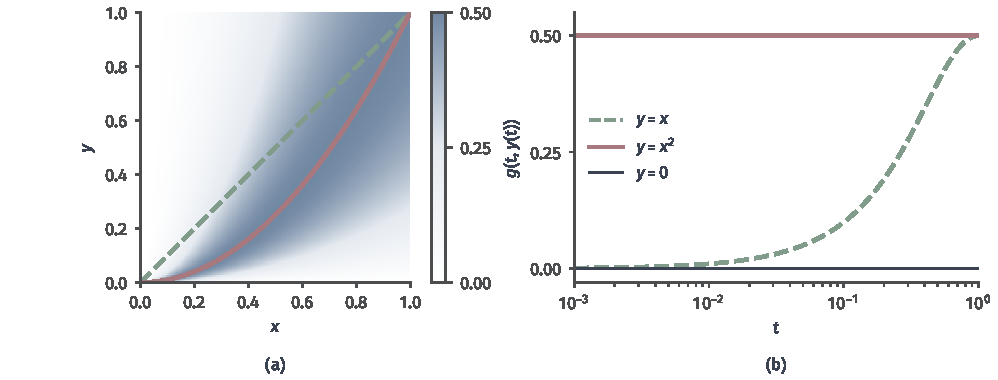
\includegraphics[width=169.0mm]{figures/00-shared/mathematical-preliminaries-upper/00-shared/matplotlib/chapter3-concept-processes/joint-limit-paths.pdf}
 \caption{取前例$g(x,y)=x^2y/(x^4+y^2)$，原点另置零。(a) 第一象限的函数值及三条路径，色阶固定为$0$至$1/2$。(b) 沿$y=0$、$y=x$分别趋零，沿$y=x^2$恒为$1/2$；横轴为正参数$t$的对数刻度，向左趋近原点。不同路径极限足以否定联合极限，有限条路径不能反向证明存在。}
 \label{fig:analysis-process-joint-limit-paths}
\end{figure*}

\paragraph{累次极限与联合极限}
另一种常见做法是逐个坐标取极限，称为累次极限。先令$y\to0$、再令$x\to0$，得到
\[
 \lim_{x\to0}\lim_{y\to0}f(x,y).
\]
内层固定$x\neq0$，让$y$单独趋于$0$；得到一个关于$x$的函数后，外层再让$x$趋于$0$。整个过程从不要求两个坐标同时趋近，因此它与联合极限是不同的问题。
对示例~\ref{ex:multivariable-path-limits}中的$f$，固定$x\neq0$时$f(x,y)\to0$，再令$x\to0$仍为$0$；交换次序同样得到$0$。两个次序的累次极限都为$0$，联合极限却不存在。

累次极限的结果还可能依赖取极限的次序。
\begin{example}[两个次序的累次极限不相等]
\label{ex:multivariable-iterated-limits-differ}
在非原点处令$h(x,y)=x^2/(x^2+y^2)$。固定$x\neq0$而令$y\to0$，得到$x^2/x^2=1$；固定$y\neq0$而令$x\to0$，得到$0$。再取外层极限，
\[
 \begin{gathered}
\lim_{x\to0}\lim_{y\to0}h(x,y)=1\\
\lim_{y\to0}\lim_{x\to0}h(x,y)=0.
 \end{gathered}
\]
内层先把一个坐标压到零，相当于先走到某条坐标轴附近，再沿坐标轴靠近原点。$h$在$x$轴上恒为$1$、在$y$轴上恒为$0$，两种次序因而给出不同结果。
\end{example}

两个例子说明：两个次序的累次极限相等，不足以推出联合极限存在；改变次序也可能改变累次极限。

反方向在补充条件下成立。若联合极限$\lim_{(x,y)\to(0,0)}f(x,y)=L$存在，并且对充分接近$0$的每个$x\neq0$，内层极限$\lim_{y\to0}f(x,y)$都存在，则累次极限$\lim_{x\to0}\lim_{y\to0}f(x,y)$也存在且等于$L$。理由是：给定$\varepsilon>0$，取联合极限定义中的$\delta$；当$0<|x|<\delta/2$、$0<|y|<\delta/2$时$|f(x,y)-L|<\varepsilon$，令$y\to0$，内层极限与$L$相差不超过$\varepsilon$。

\paragraph{统一误差估计}
要证明联合极限存在，可以寻找只依赖距离的上界。若$|f(\bm x)-L|$不超过一个只与$\lVert\bm x-\bm a\rVert_2$有关、并随距离趋于零的量，所有路径就同时受到控制。
\begin{example}[用距离上界证明联合极限]
\label{ex:multivariable-distance-bound-limit}
在非原点处考虑$x^2y/(x^2+y^2)$。由$|xy|\leq(x^2+y^2)/2$，有
\[
 \left|\frac{x^2y}{x^2+y^2}\right|
 =|x|\cdot\frac{|xy|}{x^2+y^2}
 \leq \frac{|x|}{2}
 \leq\frac12\sqrt{x^2+y^2}.
\]
给定$\varepsilon>0$，取$\delta=2\varepsilon$，则距离原点小于$\delta$的非原点都满足误差小于$\varepsilon$，因此原点处极限为$0$。

改用极坐标$(x,y)=(r\cos\theta,r\sin\theta)$，同一函数等于$r\cos^2\theta\sin\theta$，绝对值不超过$r$。这个界对所有$\theta$同时成立，给出同样的结论。
\end{example}

极坐标估计有效，关键在于这个界与角度无关。若只固定$\theta$再令$r\to0$，检查的仍然只是直线。
\begin{example}[固定角度的极坐标检验]
\label{ex:multivariable-polar-fixed-angle}
对示例~\ref{ex:multivariable-parabola-path-limit}中的$g$，代入$(x,y)=(r\cos\theta,r\sin\theta)$得到
\[
 g=\frac{r\cos^2\theta\sin\theta}{r^2\cos^4\theta+\sin^2\theta}.
\]
固定$\theta$再令$r\to0$：$\sin\theta\neq0$时分母趋于$\sin^2\theta$而分子趋于$0$，$\sin\theta=0$时函数恒为$0$，结果总是$0$。
但对每个小的$r>0$，可以取满足$\sin\theta=r\cos^2\theta$的角度。此时分子等于$r^2\cos^4\theta$、分母等于$2r^2\cos^4\theta$，函数值恰为$1/2$。这个角度随$r$改变，对应的点$(r\cos\theta,r\sin\theta)$满足$y=r^2\cos^2\theta=x^2$，正好落在抛物线上。
\end{example}

因此用极坐标证明联合极限时，需要一个对全部$\theta$同时成立、并随$r\to0$趋于零的界。

\section{连续性}
\label{sec:multivariable-continuity}

有了联合极限，就可以讨论连续：输入趋近基点时，输出趋于基点处的值。本节先给出连续性的定义，并用一致连续与Lipschitz连续量化误差的传递；再说明连续性在和、积、复合等运算下保持；最后证明闭有界集上的连续函数取到最值、一致连续。

\subsection{连续性的定义}
\label{sec:multivariable-continuity-definition}

有了联合极限，就可以定义连续：输入联合趋近基点时，输出趋于基点处的值。定义形式与一元连续性相同，只是把$|x-a|$换成输入、输出空间中的距离。
\begin{definition}[映射的连续性]
\label{def:multivariable-scalar-continuity}
设$F:D\to W$、$\bm a\in D$。若对每个$\varepsilon>0$都存在$\delta>0$，使
\[
 \bm x\in D,\quad\lVert\bm x-\bm a\rVert<\delta
 \Longrightarrow \lVert F(\bm x)-F(\bm a)\rVert<\varepsilon,
\]
则称$F$在$\bm a$处连续；在$D$上每点连续时称$F$为连续映射，标量输出时也称连续函数。
\end{definition}
条件中允许$\bm x=\bm a$。在聚点处，这等价于联合极限等于$F(\bm a)$；在孤立点处，取足够小的$\delta$使球内只有$\bm a$，定义自动成立。与极限一样，$F$连续当且仅当每个输出分量连续。
几何上，连续意味着曲面在$\bm a$上方没有裂缝或跳跃：从任何方向走近，高度都平稳地接近$f(\bm a)$。
连续函数的每条坐标切片都连续，但反过来不成立：示例~\ref{ex:multivariable-path-limits}中各条切片都连续，函数在原点却不连续。

\subsection{一致连续与Lipschitz连续}
\label{sec:multivariable-uniform-lipschitz}

连续性允许$\delta$随基点改变。有时需要在整个定义域上用同一个$\delta$统一控制误差。
\begin{definition}[一致连续]
\label{def:ls-uniform-continuity}
设$F:D\to W$。若对每个$\varepsilon>0$存在不依赖基点的$\delta>0$，使$\bm x,\bm y\in D$、$\lVert\bm x-\bm y\rVert<\delta$时$\lVert F(\bm x)-F(\bm y)\rVert<\varepsilon$，就称$F$在$D$上\term{一致连续}。
\end{definition}
有时还要给出误差的数量关系：输出的差至多是输入之差的常数倍。
\begin{definition}[Lipschitz连续]
\label{def:ls-lipschitz}
设$F:D\to W$。若存在常数$L\geq0$，使
\[
 \lVert F(\bm x)-F(\bm y)\rVert\leq L\lVert\bm x-\bm y\rVert\qquad(\bm x,\bm y\in D),
\]
就称$F$在$D$上\term{Lipschitz连续}，$L$称为Lipschitz常数。若每点都有一个邻域，使$F$在该邻域与$D$的交上Lipschitz连续，就称$F$\emph{局部Lipschitz连续}。
\end{definition}
Lipschitz连续蕴含一致连续：取$\delta=\varepsilon/L$（$L=0$时任取）即可。反过来不成立：$\sqrt x$在$[0,1]$上连续，第~\ref{sec:multivariable-closed-bounded-continuous}节将说明它一致连续，但$|\sqrt x-\sqrt0|/|x-0|=1/\sqrt x$在$x\to0^+$时无界，没有Lipschitz常数。范数本身是Lipschitz连续的，由反向三角不等式，常数为$1$。这里只说明误差界的含义；第~\ref{chap:multivariate-differentiation}章将用导数求出可微映射的Lipschitz常数。

\subsection{连续性的性质}
\label{sec:multivariable-continuity-properties}

连续性在常用运算下保持。下面逐条检验和、差、数乘、积、商、乘积型运算与复合，再用它们说明求逆在可逆矩阵上连续。

\paragraph{和的连续性}
设$f,g$在$\bm a$处连续。由三角不等式，
\[
 |(f+g)(\bm x)-(f+g)(\bm a)|\leq|f(\bm x)-f(\bm a)|+|g(\bm x)-g(\bm a)|.
\]
给定$\varepsilon>0$，分别取使两个误差都小于$\varepsilon/2$的半径，其中较小的半径就满足$f+g$的连续性要求。

\paragraph{差的连续性}
相减时两项的误差仍按三角不等式相加：$|(f-g)(\bm x)-(f-g)(\bm a)|\leq|f(\bm x)-f(\bm a)|+|g(\bm x)-g(\bm a)|$。取与和相同的半径，即得$f-g$在$\bm a$处连续。

\paragraph{数乘的连续性}
对固定实数$c$，有$|cf(\bm x)-cf(\bm a)|=|c|\,|f(\bm x)-f(\bm a)|$。$c\neq0$时，把$f$的误差控制在$\varepsilon/|c|$以内即可；$c=0$时$cf$是常函数，结论直接成立。

\paragraph{积的连续性}
若$f,g$在$\bm a$处连续，乘积的误差可以拆成两项：
\[
 f(\bm x)g(\bm x)-f(\bm a)g(\bm a)
 =f(\bm x)\bigl(g(\bm x)-g(\bm a)\bigr)+g(\bm a)\bigl(f(\bm x)-f(\bm a)\bigr).
\]
由$f$的连续性，$\bm x$足够靠近$\bm a$时$|f(\bm x)|\leq|f(\bm a)|+1$，第一项的因子$f(\bm x)$有界；两个括号又都趋于零，所以$fg$在$\bm a$处连续。这与一元的乘积极限法则是同一个论证。

坐标函数$\bm x\mapsto x_j$连续，因为$|x_j-a_j|\leq\lVert\bm x-\bm a\rVert_2$。多元多项式由坐标函数和常数经有限次加法与乘法得到，因此连续，例如$x^2+xy+y^2$。

\paragraph{商的连续性}
除法还要防止分母变为零。若再设$g(\bm a)\neq0$，由$g$的连续性，可以取一个小球使其中$|g(\bm x)|>|g(\bm a)|/2$，即$g$在基点附近远离零。于是
\[
 \left|\frac1{g(\bm x)}-\frac1{g(\bm a)}\right|
 =\frac{|g(\bm x)-g(\bm a)|}{|g(\bm x)|\,|g(\bm a)|}
 \leq\frac{2|g(\bm x)-g(\bm a)|}{g(\bm a)^2}\longrightarrow0,
\]
所以$1/g$在$\bm a$处连续，再用积的连续性得到$f/g$连续。分母非零的条件不能省略，否则商在基点没有定义；由此，有理函数在分母非零处连续。

\paragraph{内积与矩阵乘法}
向量值与矩阵值映射的乘积同样保持连续。若$F,G$在$\bm a$处连续，取值为同维向量，则$\bm x\mapsto F(\bm x)^\top G(\bm x)$在$\bm a$处连续；若$F,G$取矩阵值且形状相容，则$\bm x\mapsto F(\bm x)G(\bm x)$在$\bm a$处连续。理由是结果的每个元素都是有限个分量乘积之和，由和与积的连续性及逐分量判据得到。

\paragraph{复合映射}
若$F:D\to W$在$\bm a$处连续，映射$G$在$F(\bm a)$处连续，且$F$在$\bm a$附近的输出都在$G$的定义域内，则$G\circ F$在$\bm a$处连续。
证明分两步控制误差。给定$\varepsilon>0$，先由$G$的连续性取$\eta>0$，使中间值与$F(\bm a)$相差小于$\eta$时，$G$的输出误差小于$\varepsilon$；再由$F$的连续性取$\delta>0$，使输入距离小于$\delta$时，$F$的输出与$F(\bm a)$相差小于$\eta$。合并两步，$\lVert\bm x-\bm a\rVert<\delta$时就有$\lVert G(F(\bm x))-G(F(\bm a))\rVert<\varepsilon$。
例如$e^{-(x^2+y^2)}$和$\sqrt{1+x^2+y^2}$都是一元连续函数与多项式的复合，因而在整个平面上连续。

\paragraph{逆映射}
矩阵的函数也可以用这些规则检验。记$\mathcal G=\{\bm X\in\mathbb R^{n\times n}:\det\bm X\neq0\}$。由定理~\ref{thm:ls-adjugate-identity}，在$\mathcal G$上
\[
 \bm X^{-1}=\frac{\operatorname{adj}(\bm X)}{\det\bm X}.
\]
$\det\bm X$与$\operatorname{adj}(\bm X)$的每个元素都是$\bm X$各元素的多项式，因而连续；在$\mathcal G$上分母非零，由商的连续性，$\bm X^{-1}$的每个元素都连续。由逐分量判据，求逆$\bm X\mapsto\bm X^{-1}$在可逆矩阵集合上连续。

\subsection{闭有界集上的连续函数}
\label{sec:multivariable-closed-bounded-continuous}

连续性的一个重要用途是保证最值存在。机器学习中常在一块参数区域内最小化损失；如果最小值根本取不到，“求最小点”就没有对象。
一元情形中，闭区间上的连续函数一定取到最值，关键事实是闭区间内任意点列都有收敛于该区间内的子列。第~\ref{sec:multivariable-bolzano-weierstrass-section}节已把这一子列性质推广到有限维闭有界集（定理~\ref{thm:multivariable-bolzano-weierstrass}），本小节用它得到多元极值定理和一致连续性。矩阵空间把元素排成向量后是$\mathbb R^{mn}$，结论相同。

\paragraph{有界性与极值达到}
要让上、下确界由定义域内的点取得，必须防止函数值趋近确界的输入序列逃出定义域。这样的序列可能跑向无穷远，也可能趋向一个不属于定义域的边界点。闭有界集的子列性质同时排除了这两种情况。
\begin{theorem}[闭有界集上的极值定理]
\label{thm:multivariable-extreme-value}
\phantomsection\label{thm:ls-extreme-value}
设$K\subseteq\mathbb R^d$非空、闭且有界，$f:K\to\mathbb R$连续，则$f$有界，且存在$\bm x_{\min},\bm x_{\max}\in K$满足
\[
 f(\bm x_{\min})\leq f(\bm x)\leq f(\bm x_{\max})\qquad(\bm x\in K).
\]
\end{theorem}
\begin{proof}
一元闭区间上最值定理的证明只用到两件事：定义域内任意点列有收敛于定义域内的子列，以及函数连续。
这里的$K$由定理~\ref{thm:multivariable-bolzano-weierstrass}满足同一子列条件，输出仍为实数，所以该证明逐字适用。例如对最大值，取$\bm x_n\in K$使$f(\bm x_n)$趋于上确界，选出收敛子列$\bm x_{n_k}\to\bm x_{\max}\in K$，连续性给出$f(\bm x_{\max})$等于上确界。
\end{proof}
定理的条件只是充分条件，但删去其中任何一个，结论都可能失败。与一元情形一样，可以逐项构造反例。
\begin{example}[删去闭性、有界性或连续性时最值可能取不到]
\label{ex:multivariable-extreme-value-failures}
在开单位圆盘$\{x^2+y^2<1\}$上，连续函数$f(x,y)=x^2+y^2$的上确界为$1$，但趋近上确界的点跑向不属于圆盘的边界圆，最大值取不到；这说明不能删去闭性。
在闭而无界的整个平面上，$f(x,y)=-(x^2+y^2)$在远处无限变小，没有下界；这说明不能删去有界性。
在闭单位圆盘上，令$f(x,y)=x^2+y^2$（$x^2+y^2<1$），并在边界圆上令$f=0$。定义域闭且有界，但$f$在边界圆上不连续，上确界$1$仍取不到；这说明不能删去连续性。
\end{example}

\paragraph{一致连续性}
一元情形中，闭区间上的连续函数一致连续。同样，闭有界集上的连续映射一致连续（定义~\ref{def:ls-uniform-continuity}），证明仍然只用子列性质。
\begin{theorem}[闭有界集上的一致连续性]
\label{thm:multivariable-uniform-continuity}
设$K\subseteq\mathbb R^d$非空、闭且有界，$F:K\to W$连续，则$F$在$K$上一致连续。
\end{theorem}
\begin{proof}
若不然，存在$\varepsilon_0>0$，使每个$\delta=1/n$都对应$\bm x_n,\bm y_n\in K$，满足$\lVert\bm x_n-\bm y_n\rVert<1/n$而$\lVert F(\bm x_n)-F(\bm y_n)\rVert\geq\varepsilon_0$。由定理~\ref{thm:multivariable-bolzano-weierstrass}取收敛子列$\bm x_{n_k}\to\bm x\in K$，则$\lVert\bm y_{n_k}-\bm x\rVert\leq\lVert\bm y_{n_k}-\bm x_{n_k}\rVert+\lVert\bm x_{n_k}-\bm x\rVert\to0$。由$F$在$\bm x$处连续，$F(\bm x_{n_k})$与$F(\bm y_{n_k})$都趋于$F(\bm x)$，两者之差趋于零，与$\varepsilon_0$矛盾。
\end{proof}
第~\ref{chap:region-integrals}章的Riemann和、参数积分与换元，都要在整个区域上统一控制局部近似的误差，用到的正是一致连续性。

\section{矩阵范数与商范数}
\label{sec:ls-derived-norms}

有了范数与前几节的结论，就可以在由已有空间构造出的新空间上定义范数。矩阵（线性映射）组成的空间上，诱导矩阵范数衡量最大放大倍数；商空间上，商范数衡量忽略一个子空间中的差别以后剩下的大小。两者都是定义，它们的上确界或下确界有限、可以取到，用的正是范数等价、闭有界集上的最值与子空间的闭性。线性泛函组成的对偶空间上的对偶范数，放到第~\ref{chap:dual-spaces}章与对偶空间一起讨论。

\subsection{矩阵范数}
\label{sec:ls-matrix-norms}
\label{sec:ch06-map-comparison}
\label{sec:matrix-analysis-norms-effective-rank}
\label{sec:multivariable-operator-norm}

第~\ref{chap:linear-operations}章用Frobenius范数衡量矩阵元素的总体大小。误差分析更常用另一种大小：把矩阵看作映射$\bm x\mapsto\bm A\bm x$，问它最多把输入放大多少倍。

\paragraph{诱导矩阵范数}
设$\bm A\in\mathbb R^{m\times d}$，在$\mathbb R^d$上取输入范数$\lVert\cdot\rVert_\alpha$，在$\mathbb R^m$上取输出范数$\lVert\cdot\rVert_\beta$，两者可以是任意范数。
\begin{definition}[由向量范数诱导的矩阵范数]
\label{def:matrix-analysis-induced-norm}
$\bm A$的\term{诱导矩阵范数}（induced matrix norm）为
\[
 \lVert\bm A\rVert_{\alpha\to\beta}
 =\sup_{\lVert\bm x\rVert_\alpha\leq1}\lVert\bm A\bm x\rVert_\beta .
\]
两端采用同一类$p$范数时简写为$\lVert\bm A\rVert_p$。
\end{definition}
$d\geq1$时，由齐次性，上确界也等于$\sup_{\bm x\neq\bm0}\lVert\bm A\bm x\rVert_\beta/\lVert\bm x\rVert_\alpha$：单位球内的非零$\bm x$满足$\lVert\bm A\bm x\rVert_\beta\leq\lVert\bm A(\bm x/\lVert\bm x\rVert_\alpha)\rVert_\beta$，零向量的贡献为零。定义域为零空间时规定范数为零。

下面先证明这个上确界有限，并由此得到线性作用的连续性。

\subsubsection{线性作用的连续性}
\label{sec:ls-linear-action-continuity}

把矩阵作用看作映射$\bm x\mapsto\bm A\bm x$，诱导范数正是它放大输入的倍数上界，因而也给出连续性的定量形式。
\begin{theorem}[线性作用的连续性]
\label{thm:ls-linear-map-continuity}
设$\bm A\in\mathbb R^{m\times d}$，$\mathbb R^d$与$\mathbb R^m$上分别取范数$\lVert\cdot\rVert_\alpha$与$\lVert\cdot\rVert_\beta$，则：
\begin{enumerate}
 \item 诱导范数$\lVert\bm A\rVert_{\alpha\to\beta}$有限，并且对一切$\bm x$有$\lVert\bm A\bm x\rVert_\beta\leq\lVert\bm A\rVert_{\alpha\to\beta}\lVert\bm x\rVert_\alpha$；
 \item $\bm x\mapsto\bm A\bm x$是Lipschitz连续的：$\lVert\bm A\bm x-\bm A\bm y\rVert_\beta\leq\lVert\bm A\rVert_{\alpha\to\beta}\lVert\bm x-\bm y\rVert_\alpha$；
 \item 定义中的上确界可以取到：存在$\lVert\bm x^\star\rVert_\alpha\leq1$，使$\lVert\bm A\bm x^\star\rVert_\beta=\lVert\bm A\rVert_{\alpha\to\beta}$。
\end{enumerate}
\end{theorem}
\begin{proof}
第一条。把$\bm A\bm x$按列展开，由三角不等式与齐次性，
\[
 \lVert\bm A\bm x\rVert_\beta=\Bigl\lVert\sum_jx_j\bm A\bm e_j\Bigr\rVert_\beta\leq\sum_j|x_j|\,\lVert\bm A\bm e_j\rVert_\beta\leq\Bigl(\max_j\lVert\bm A\bm e_j\rVert_\beta\Bigr)\lVert\bm x\rVert_1 .
\]
由范数等价，存在常数$c$使$\lVert\bm x\rVert_1\leq c\lVert\bm x\rVert_\alpha$，所以$\lVert\bm A\bm x\rVert_\beta\leq C\lVert\bm x\rVert_\alpha$，其中$C=c\max_j\lVert\bm A\bm e_j\rVert_\beta$。于是单位球上的$\lVert\bm A\bm x\rVert_\beta$不超过$C$，上确界有限。对$\bm x\neq\bm0$，$\bm x/\lVert\bm x\rVert_\alpha$在单位球上，由齐次性得所述不等式；$\bm x=\bm0$时两边都为零。

第二条。把第一条用于$\bm x-\bm y$，并利用$\bm A\bm x-\bm A\bm y=\bm A(\bm x-\bm y)$即得。

第三条。单位球$\{\bm x:\lVert\bm x\rVert_\alpha\leq1\}$是闭集，由范数等价又是有界集。函数$\bm x\mapsto\lVert\bm A\bm x\rVert_\beta$是连续的矩阵作用与连续的范数的复合，由极值定理~\ref{thm:multivariable-extreme-value}，它在单位球上取到最大值。
\end{proof}
第一条说明，诱导范数是使$\lVert\bm A\bm x\rVert_\beta\leq C\lVert\bm x\rVert_\alpha$对全部$\bm x$成立的最小常数：比它小的常数在取到最大值的$\bm x^\star$处就不成立。第二条按定义~\ref{def:ls-lipschitz}把这个常数读作误差放大的上界：输入相差$\lVert\bm x-\bm y\rVert_\alpha$时，输出至多相差它的$\lVert\bm A\rVert_{\alpha\to\beta}$倍。第三条使定义中的$\sup$可以写成$\max$。

\paragraph{线性映射的算子范数}
对有限维赋范空间之间的线性映射$T:V\to W$，同样定义\term{算子范数}（operator norm）
\[
 \lVert T\rVert=\sup_{\lVert\bm v\rVert_V\leq1}\lVert T\bm v\rVert_W .
\]
选定$V,W$的基，并把$V,W$原有的范数搬到坐标空间（第~\ref{sec:ls-normed-space-definition}节借助坐标定义范数的方法），$T$由矩阵$\bm A$表示，而$\lVert T\rVert$恰等于$\bm A$在这两个坐标范数下的诱导范数。由定理~\ref{thm:ls-linear-map-continuity}，算子范数有限并可以取到，有限维空间之间的线性映射都Lipschitz连续。换基而保持原空间的范数时，数值不变；若改为在坐标上指定另一种范数，就改变了大小的计量规则。

\subsubsection{常用的诱导范数}
\label{sec:ls-common-induced-norms}

诱导范数与把矩阵看作元素数组的Frobenius范数不同。常用的诱导范数有三种。

前两种可以直接从元素算出：
\[
 \begin{gathered}
 \lVert\bm A\rVert_1=\max_j\sum_i|a_{i,j}|,\\
 \lVert\bm A\rVert_\infty=\max_i\sum_j|a_{i,j}|,
 \end{gathered}
\]
即最大绝对列和与最大绝对行和，推导见下面的“列和与行和公式”。

第三种是诱导$2$范数，也称\term{谱范数}（spectral norm），
\[
 \lVert\bm A\rVert_2=\sup_{\lVert\bm x\rVert_2=1}\lVert\bm A\bm x\rVert_2,
\]
它等于最大奇异值，计算要用到第~\ref{chap:singular-value-decomposition}章的奇异值分解。下面在同一个矩阵上比较两种诱导范数与Frobenius范数。
\begin{example}[同一矩阵在不同口径下的大小]
\label{ex:ls-matrix-norms-shear}
以剪切矩阵
\[
 \bm A=\begin{bmatrix}1&1\\0&1\end{bmatrix}
\]
为例。按列和公式，两列的绝对值之和分别为$1+0=1$与$1+1=2$；按行和公式，两行的绝对值之和分别为$1+1=2$与$0+1=1$；Frobenius范数则把全部元素的平方相加，得$1+1+0+1=3$。所以
\[
 \begin{gathered}
 \lVert\bm A\rVert_1=\max\{1,2\}=2,\\
 \lVert\bm A\rVert_\infty=\max\{2,1\}=2,\\
 \lVert\bm A\rVert_{\mathrm F}=\sqrt3.
 \end{gathered}
\]
$\lVert\bm A\rVert_1$与$\lVert\bm A\rVert_\infty$在这里碰巧相等，但分别由第二列和第一行取得，回答的是不同输入范数下的最大放大倍数；Frobenius范数只汇总元素大小，又给出另一个数值。谈论矩阵“多大”时，须说明所用的口径。
\end{example}
谱范数也有直观的几何意义。如图~\ref{fig:ls-induced-norm-action}，单位圆被$\bm A$拉成椭圆，椭圆最长半轴的长度就是最大放大倍数。
\begin{figure*}[htbp]
  \centering
  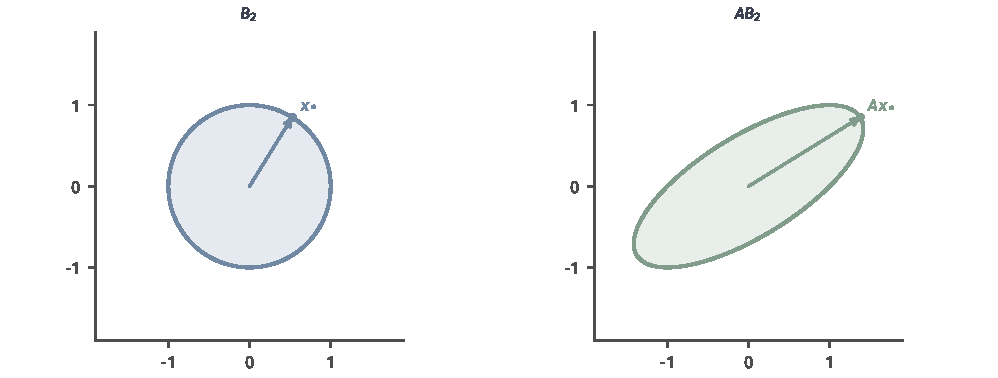
\includegraphics[width=169mm]{figures/00-shared/mathematical-preliminaries-upper/02-linear-spaces/matplotlib/ls-induced-norm-action/ls-induced-norm-action.pdf}
  \caption{诱导矩阵范数衡量最坏放大倍数。左：单位圆$\lVert\bm x\rVert_2=1$；中：线性作用$\bm A$把单位圆映成椭圆；右：椭圆最长的半轴长度就是$\lVert\bm A\rVert_2$，箭头指示最大放大方向。数值由$\bm A$的教学构造直接得到，是解析例。}
  \label{fig:ls-induced-norm-action}
\end{figure*}

\subsubsection{矩阵范数的性质}

有限性与可达性已由定理~\ref{thm:ls-linear-map-continuity}得到。本小节依次求出具体公式、核对范数公理，再给出乘积的上界；这些显式估计用于计算实际的误差常数。

\paragraph{列和与行和公式}
第一式按列计算：
\[
 \lVert\bm A\bm x\rVert_1=\Bigl\lVert\sum_jx_j\bm A_{:,j}\Bigr\rVert_1\leq\sum_j|x_j|\,\lVert\bm A_{:,j}\rVert_1\leq\Bigl(\max_j\lVert\bm A_{:,j}\rVert_1\Bigr)\lVert\bm x\rVert_1.
\]
取$\bm x$为最大绝对列和所在列对应的标准坐标向量时，等号成立。第二式按行计算：对每个$i$，
\[
 |(\bm A\bm x)_i|\leq\sum_j|a_{i,j}|\,|x_j|\leq\Bigl(\sum_j|a_{i,j}|\Bigr)\lVert\bm x\rVert_\infty,
\]
对$i$取最大值即得上界。取输入各坐标为最大绝对行和那一行元素的符号（元素为零处取$1$），等号成立。

\paragraph{谱范数不超过Frobenius范数}
谱范数需要奇异值才能精确计算，但Frobenius范数给出一个容易计算的上界：
\[
 \begin{gathered}
 \lVert\bm A\bm x\rVert_2\leq\lVert\bm A\rVert_{\mathrm F}\lVert\bm x\rVert_2,\\
 \lVert\bm A\rVert_2\leq\lVert\bm A\rVert_{\mathrm F}.
 \end{gathered}
\]
对每行用$p=q=2$的Hölder不等式，得$(\bm A\bm x)_i^2=(\bm A_{i,:}\bm x)^2\leq\lVert\bm A_{i,:}\rVert_2^2\lVert\bm x\rVert_2^2$。对$i$求和，右侧的$\sum_i\lVert\bm A_{i,:}\rVert_2^2$正是$\lVert\bm A\rVert_{\mathrm F}^2$，于是得到第一式。第一式说明每个比值$\lVert\bm A\bm x\rVert_2/\lVert\bm x\rVert_2$都不超过$\lVert\bm A\rVert_{\mathrm F}$，由此得到第二式。

\paragraph{诱导范数是范数}
诱导范数满足范数的各条要求。非负性与齐次性由定义直接得到。若$\lVert\bm A\rVert_{\alpha\to\beta}=0$，则每个$\bm A\bm e_j=\bm0$，即$\bm A=\bm0$，这给出正定性。三角不等式来自$\lVert(\bm A+\bm B)\bm x\rVert_\beta\leq\lVert\bm A\bm x\rVert_\beta+\lVert\bm B\bm x\rVert_\beta$，两边除以$\lVert\bm x\rVert_\alpha$再取上确界即得。

\paragraph{次乘性}
诱导范数还能控制乘积。中间范数匹配时，
\[
 \lVert\bm A\bm B\rVert_{\alpha\to\gamma}
 \leq\lVert\bm A\rVert_{\beta\to\gamma}
 \lVert\bm B\rVert_{\alpha\to\beta}.
\]
这只需连续应用两次诱导范数的界：
\[
 \lVert\bm A\bm B\bm x\rVert_\gamma\leq\lVert\bm A\rVert_{\beta\to\gamma}\lVert\bm B\bm x\rVert_\beta\leq\lVert\bm A\rVert_{\beta\to\gamma}\lVert\bm B\rVert_{\alpha\to\beta}\lVert\bm x\rVert_\alpha.
\]
两边除以$\lVert\bm x\rVert_\alpha$再取上确界即得。反复使用可得$\lVert\bm A^k\rVert_p\leq\lVert\bm A\rVert_p^k$。

\paragraph{Frobenius范数与谱范数的混合界}
乘积的Frobenius范数可以用一个因子的谱范数和另一个因子的Frobenius范数控制：
\begin{equation}
\begin{gathered}
\lVert\bm A\bm B\rVert_{\mathrm F}
 \leq\lVert\bm A\rVert_2\lVert\bm B\rVert_{\mathrm F},\\
\lVert\bm A\bm B\rVert_{\mathrm F}
 \leq\lVert\bm A\rVert_{\mathrm F}\lVert\bm B\rVert_2.
\end{gathered}
\label{eq:matrix-analysis-mixed-submultiplicativity}
\end{equation}
第一式按列计算：
\[
 \lVert\bm A\bm B\rVert_{\mathrm F}^2=\sum_j\lVert\bm A\bm B_{:,j}\rVert_2^2\leq\lVert\bm A\rVert_2^2\sum_j\lVert\bm B_{:,j}\rVert_2^2=\lVert\bm A\rVert_2^2\lVert\bm B\rVert_{\mathrm F}^2.
\]
第二式对转置应用第一式：$\lVert\bm A\bm B\rVert_{\mathrm F}=\lVert\bm B^\top\bm A^\top\rVert_{\mathrm F}\leq\lVert\bm B^\top\rVert_2\lVert\bm A^\top\rVert_{\mathrm F}$。转置不改变Frobenius范数，还需要说明$\lVert\bm B^\top\rVert_2=\lVert\bm B\rVert_2$。对固定的$\bm x$，由$p=q=2$的Hölder不等式，$\lVert\bm y\rVert_2=1$时$|\bm y^\top\bm B\bm x|\leq\lVert\bm B\bm x\rVert_2$；$\bm B\bm x\neq\bm0$时取$\bm y=\bm B\bm x/\lVert\bm B\bm x\rVert_2$即取等号。所以
\[
 \lVert\bm B\rVert_2=\sup_{\lVert\bm x\rVert_2=\lVert\bm y\rVert_2=1}|\bm y^\top\bm B\bm x|.
\]
由于$\bm y^\top\bm B\bm x=\bm x^\top\bm B^\top\bm y$，交换$\bm x,\bm y$的角色，同一个上确界也等于$\lVert\bm B^\top\rVert_2$。再结合$\lVert\bm A\rVert_2\leq\lVert\bm A\rVert_{\mathrm F}$，可知Frobenius范数也满足次乘性：$\lVert\bm A\bm B\rVert_{\mathrm F}\leq\lVert\bm A\rVert_{\mathrm F}\lVert\bm B\rVert_{\mathrm F}$。

\subsection{商范数}
\label{sec:ls-quotient-norms}

子空间的闭性还可以用来给商空间定义范数。第~\ref{sec:ls-quotient-spaces}节的商空间$V/U$把相差$U$中向量的点看成同一个类$\bm x+U$，那里只建立了线性结构。要度量一个类的大小，自然的选择是类中的点到$U$的距离。这个距离不依赖类中代表元的选取：若$\bm x'=\bm x+\bm u_0$，$\bm u_0\in U$，则$\bm u$遍历$U$时$\bm u-\bm u_0$也遍历$U$，所以$d(\bm x',U)=d(\bm x,U)$。于是可以定义\term{商范数}（quotient norm）
\[
 \lVert\bm x+U\rVert_{V/U}=d(\bm x,U)=\inf_{\bm u\in U}\lVert\bm x-\bm u\rVert .
\]

它满足范数的三条要求。三角不等式：对任意$\bm u,\bm u'\in U$，
\[
 d(\bm x+\bm y,U)\leq\lVert(\bm x-\bm u)+(\bm y-\bm u')\rVert\leq\lVert\bm x-\bm u\rVert+\lVert\bm y-\bm u'\rVert;
\]
取$\bm u,\bm u'$使右侧两项分别任意接近$d(\bm x,U)$与$d(\bm y,U)$，即得$d(\bm x+\bm y,U)\leq d(\bm x,U)+d(\bm y,U)$。齐次性：$c\neq0$时$cU=U$，所以$d(c\bm x,U)=|c|\,d(\bm x,U)$；$c=0$时两边都为零。正定性要求$d(\bm x,U)=0$只在$\bm x+U=U$即$\bm x\in U$时发生，这正是前面由子空间闭性得到的结论。在子空间不一定闭的更一般空间中，同一个公式可能只给出半范数，有限维的结论不能无条件外推。

\paragraph{一般范数下的最近点}
商范数是一个下确界。这个下确界能否取到，就是$U$中是否存在离给定点最近的点。
\begin{theorem}[最近点的存在]
\label{thm:multivariable-nearest-point-existence}
设$V$是有限维赋范空间，$U$是子空间，$\bm x\in V$，则存在$\bm u^\star\in U$，使$\lVert\bm x-\bm u^\star\rVert=d(\bm x,U)$。
\end{theorem}
\begin{proof}
在$U$中取$\bm u_k$，使$\lVert\bm x-\bm u_k\rVert\to d(\bm x,U)$。由$\lVert\bm u_k\rVert\leq\lVert\bm x\rVert+\lVert\bm x-\bm u_k\rVert$，序列$(\bm u_k)$有界。由定理~\ref{thm:multivariable-bolzano-weierstrass}（范数等价使它对任意范数适用），存在收敛子列$\bm u_{k_i}\to\bm u^\star$；由子空间闭性，$\bm u^\star\in U$。范数连续，所以$\lVert\bm x-\bm u^\star\rVert=\lim_i\lVert\bm x-\bm u_{k_i}\rVert=d(\bm x,U)$。
\end{proof}
最近点存在，却可能不唯一。
\begin{example}[反例：$\ell_\infty$范数下最近点不唯一]
\label{ex:ls-linf-nonunique-nearest}
在$\mathbb R^2$上取$\ell_\infty$范数，求点$\bm y=(0,1)^\top$到横轴$U=\operatorname{span}\{(1,0)^\top\}$的最近点。$U$中的点写成$(t,0)^\top$，差向量为$(-t,1)^\top$，于是
\[
 \lVert\bm y-(t,0)^\top\rVert_\infty=\max\{|t|,1\}\geq1,
\]
等号当且仅当$|t|\leq1$时成立。

所以$d(\bm y,U)=1$，而且横轴上整整一段$|t|\leq1$的点$(t,0)^\top$都是最近点。原因在于$\ell_\infty$只看最大坐标：竖直方向的差已经是$1$，水平方向的差只要不超过$1$，就不影响距离。欧氏范数下只有$t=0$达到最小距离，可见最近点是否唯一取决于所用的范数，而不只取决于点和子空间。
\end{example}
加入内积以后，第~\ref{sec:ls-orthogonal-projection}节将证明正交投影给出唯一的最近点。一般范数下的存在性与内积几何下的唯一性，回答的是两个不同的问题。


\section{本章小结}
\label{sec:ls-normed-spaces-summary}
\phantomsection
\label{sec:ls-normed-inner-product-summary}

本章回答了章首的两个问题：两个向量相差多少，一列近似是否趋于极限。两者都由范数回答。

范数给向量规定大小，从而可以度量误差。常用坐标范数之间满足$\lVert\bm x\rVert_q\leq\lVert\bm x\rVert_p\leq d^{1/p-1/q}\lVert\bm x\rVert_q$（$p\leq q$），比较常数依赖维数，所以同一个误差在不同范数下的读数不同。

有限维空间中任意两个范数等价，所以开集、闭集、有界集、收敛、柯西性质与连续都不依赖所选范数，变的只是误差的数值和比较常数。

有了这些概念就能谈收敛与连续。向量列与矩阵列的收敛等价于逐坐标、逐元素收敛；有限维赋范空间在任意范数下完备，是Banach空间，因而绝对收敛的向量与矩阵级数收敛，并有尾和估计。映射的联合极限要求所有趋近方式给出同一结果，只检查若干路径只能否定、不能证明极限存在。闭有界集上的连续函数取到最值并且一致连续，闭性、有界性与连续性三个条件缺一不可；有限维子空间都是闭集。

在此基础上可以定义导出的范数：诱导矩阵范数给出线性映射的最大放大倍数，有限维线性映射因而都Lipschitz连续；商范数衡量忽略一个子空间中的差别以后剩余的大小。一般范数下向子空间的最近点存在，但可能不唯一；唯一性要等第~\ref{chap:inner-product-spaces}章的内积给出。

这些结论都依赖有限维：范数等价、完备性与最近点存在的证明，都用到了有限个坐标或闭有界集上的最值。它们为后续各章提供共同依据：矩阵幂和级数使用收敛与次乘性，迭代使用完备性和误差估计，多元微分把局部变化表示为线性映射并用算子范数控制余项。


\chapter{内积空间}
\label{chap:inner-product-spaces}

范数只度量大小，不给出角度。一般范数下谈不上两个方向是否垂直，向子空间的最近点也可能不唯一（示例~\ref{ex:ls-linf-nonunique-nearest}）。第~\ref{chap:linear-operations}章在$\mathbb R^d$上用逐项相乘再求和定义了欧氏内积，并由它得到长度和夹角。本章提取这种计算的共同规则，在一般线性空间上定义内积，并回答三个问题：两个方向是否垂直、夹角多大，一个向量在子空间中最好的近似是什么，以及怎样选基才能让坐标计算最简单。

前三节从内积出发逐步得到几何量。第~\ref{sec:ls-inner-product-axioms}节给出内积的公理、例子与复内积的约定；第~\ref{sec:ls-inner-product-angle}节由内积定义长度与正交，证明Cauchy--Schwarz不等式，并由它定义夹角；第~\ref{sec:ls-inner-product-distance}节证明内积诱导的长度满足三角不等式，因而是范数并给出距离，再用平行四边形恒等式说明并非每个范数都来自内积。

后两节把这些几何量写成可以计算的形式。第~\ref{sec:ls-gram-psd}节用Gram矩阵记录一组向量的两两内积，说明Gram矩阵恰好是全部半正定矩阵，并用基的Gram矩阵写出坐标下的内积。第~\ref{sec:ls-orthogonality-and-projection}节研究正交分解与标准正交基，用Gram--Schmidt正交化构造标准正交基，证明正交投影是子空间中唯一的最近点。

本章依赖第~\ref{chap:linear-representation}章的基、坐标与线性映射，以及第~\ref{chap:normed-spaces}章的范数、收敛与有限维性质。全章只讨论有限维空间。内积把线性泛函表示为与固定向量的内积、把对偶映射改写为伴随，这些内容放在第~\ref{chap:dual-spaces}章。

% 内积空间：内积的定义（公理、例子、复内积的约定）。

\section{内积的定义}
\label{sec:ls-inner-product-axioms}
\phantomsection
\label{sec:ls-inner-product-spaces}
\label{sec:ls-inner-product-definition}

欧氏内积对每个变量都保持线性组合，交换两个变量不改变结果，向量与自身的内积只在零向量处为零。这些性质只涉及线性运算，因此可以用来定义一般空间上的内积。
\begin{definition}[内积空间]
\label{def:functional-inner-product-space}
\label{def:linear-algebra-inner-product}
设$V$是实线性空间。映射$\langle\cdot,\cdot\rangle:V\times V\to\mathbb R$若对任意$\bm x,\bm y,\bm z\in V$与$a,b\in\mathbb R$满足
\begin{enumerate}
 \item 双线性：$\langle a\bm x+b\bm y,\bm z\rangle=a\langle\bm x,\bm z\rangle+b\langle\bm y,\bm z\rangle$，且$\langle\bm z,a\bm x+b\bm y\rangle=a\langle\bm z,\bm x\rangle+b\langle\bm z,\bm y\rangle$；
 \item 对称性：$\langle\bm x,\bm y\rangle=\langle\bm y,\bm x\rangle$；
 \item 正定性：$\langle\bm x,\bm x\rangle\geq0$，且$\langle\bm x,\bm x\rangle=0$当且仅当$\bm x=\bm0$，
\end{enumerate}
就称为$V$上的\term{内积}（inner product）；配备内积的线性空间$(V,\langle\cdot,\cdot\rangle)$称为\term{内积空间}（inner-product space）。
\end{definition}

\paragraph{内积的例子}
先检验欧氏内积满足这三条公理。设$\bm x,\bm y,\bm z\in\mathbb R^d$，$a,b\in\mathbb R$。对称性成立，因为每一项$x_jy_j=y_jx_j$。对第一个变量的线性来自有限和的运算法则：
\[
 \sum_j(ax_j+bz_j)y_j=a\sum_jx_jy_j+b\sum_jz_jy_j,
\]
再由对称性，对第二个变量同样成立。正定性成立，因为$\langle\bm x,\bm x\rangle=\sum_jx_j^2\geq0$，而非负数之和为零时每一项都为零。

同形矩阵上的Frobenius内积也满足三条公理。它对两个变量分别线性；交换两个矩阵不改变各项乘积，因而对称；$\langle\bm A,\bm A\rangle_{\mathrm F}=\sum_{i,j}a_{i,j}^2$非负，并且只在$\bm A=\bm0$时为零。这正是把$mn$个元素看作坐标时欧氏内积的三条性质。所以下面从公理推出的一般结论对它同样成立。

标准内积之外，一般空间上还可以有各种内积。下面在$P_1$上规定一个只看两点取值的内积，后面的算例会反复用到它。
\begin{example}[只看两点取值的内积]
\label{ex:ls-two-point-inner-product}
在$P_1$上规定
\[
 \langle f,g\rangle=f(0)g(0)+f(1)g(1),
\]
即把两个函数在$t=0,1$处的取值配对相乘再相加。函数值$f(0)$、$f(1)$都随$f$线性变化，所以右端对$f$与对$g$分别线性；交换$f,g$不改变右端，对称性也成立。

正定性要用到$P_1$的特点。由
\[
 \langle f,f\rangle=f(0)^2+f(1)^2\geq0,
\]
若它为零，则$f(0)=f(1)=0$；对$f=a+bt$，这就是$a=0$、$a+b=0$，故$f=0$。一次多项式由两个点的取值确定，这一步才能成立。

因此这一规则是$P_1$上的内积。它与系数向量$(a,b)^\top$的欧氏内积并不相同：例如$\langle1,t\rangle=1\cdot0+1\cdot1=1$，而$1$与$t$的系数向量$(1,0)^\top$、$(0,1)^\top$的欧氏内积为零。同一对函数是否正交，要看采用哪种内积。
\end{example}

\paragraph{复内积的约定}
上面的定义针对实空间。在复空间中，若两个变量都按复数线性，并且满足实数式的对称性，那么$\langle\mathrm i\bm x,\mathrm i\bm x\rangle=-\langle\bm x,\bm x\rangle$，无法对非零向量保持正定。因此复内积采用另一种约定：对第一个变量共轭线性，对第二个变量线性，并满足$\langle\bm x,\bm y\rangle=\overline{\langle\bm y,\bm x\rangle}$。标准例子是$\langle\bm x,\bm y\rangle=\bm x^*\bm y$，其中$\bm x^*$表示共轭转置；仍要求$\langle\bm x,\bm x\rangle>0$对非零$\bm x$成立。

后面的Cauchy--Schwarz不等式在复内积下同样成立。若$\bm y\ne\bm0$，在$\lVert\bm x-\alpha\bm y\rVert^2\geq0$中取$\alpha=\langle\bm y,\bm x\rangle/\lVert\bm y\rVert^2$，展开可得
\[
 |\langle\bm x,\bm y\rangle|^2\leq\lVert\bm x\rVert^2\lVert\bm y\rVert^2 .
\]
因此它的平方根仍给出范数。

但复内积的值可能不是实数，下一节用余弦定义夹角的公式不能直接照搬。下文的证明继续使用实内积，复情形需要把转置相应改为共轭转置。

% 内积空间：由内积定义的长度、正交、Cauchy--Schwarz不等式与夹角。

\section{由内积定义的夹角}
\label{sec:ls-inner-product-angle}

\paragraph{长度与正交}
与$\mathbb R^d$中一样，内积给出长度$\lVert\bm v\rVert=\sqrt{\langle\bm v,\bm v\rangle}$，它是否满足范数的全部要求，留到下一节检验；$\langle\bm x,\bm y\rangle=0$时称$\bm x,\bm y$正交。正交的两个向量满足勾股定理。展开
\[
 \lVert\bm x+\bm y\rVert^2=\lVert\bm x\rVert^2+2\langle\bm x,\bm y\rangle+\lVert\bm y\rVert^2,
\]
交叉项为零，得$\lVert\bm x+\bm y\rVert^2=\lVert\bm x\rVert^2+\lVert\bm y\rVert^2$。

\paragraph{Cauchy--Schwarz不等式}
平面上两个非零向量的夹角$\theta$满足
\[
 \langle\bm x,\bm y\rangle=\lVert\bm x\rVert\,\lVert\bm y\rVert\cos\theta.
\]
要在一般内积空间中反过来用这个关系定义夹角，须先保证内积除以两个长度之积后总落在$[-1,1]$中。下面的不等式给出这一保证。
\begin{theorem}[Cauchy--Schwarz不等式]
\label{thm:linear-algebra-cauchy-schwarz}
对任一内积及其长度，任意向量$\bm x,\bm y$满足
\begin{equation}
 |\langle\bm x,\bm y\rangle|\leq\lVert\bm x\rVert\,\lVert\bm y\rVert,
 \label{eq:prelim-cauchy-schwarz}
\end{equation}
等号成立当且仅当其中一个向量是另一个向量的实数倍。
\end{theorem}
\begin{proof}
$\bm y=\bm0$时两边都为零。设$\bm y\neq\bm0$。对任意实数$s$，向量$\bm x-s\bm y$的长度平方非负；按内积的对称性与双线性展开，
\[
 0\leq\lVert\bm x-s\bm y\rVert^2
 =\lVert\bm x\rVert^2-2s\langle\bm x,\bm y\rangle+s^2\lVert\bm y\rVert^2.
\]
右侧是$s$的二次函数，二次项系数为正，在顶点$s=\langle\bm x,\bm y\rangle/\lVert\bm y\rVert^2$处最小，最小值为$\lVert\bm x\rVert^2-\langle\bm x,\bm y\rangle^2/\lVert\bm y\rVert^2$。它非负，两边乘以$\lVert\bm y\rVert^2$再开平方，即得不等式。等号成立当且仅当对这个$s$有$\bm x-s\bm y=\bm0$，即$\bm x$是$\bm y$的实数倍；连同$\bm y=\bm0$的情形，即得等号条件。
\end{proof}
证明只用了内积的三条公理，所以不等式对每一种内积都成立。在$\mathbb R^d$的标准内积下，它就是$p=q=2$的Hölder不等式（定理~\ref{thm:linear-algebra-holder}）；对Frobenius内积，它给出$|\langle\bm A,\bm B\rangle_{\mathrm F}|\leq\lVert\bm A\rVert_{\mathrm F}\lVert\bm B\rVert_{\mathrm F}$。

\paragraph{夹角}
由Cauchy--Schwarz不等式，非零向量的夹角$\theta\in[0,\pi]$可以由
\[
 \cos\theta=\frac{\langle\bm x,\bm y\rangle}{\lVert\bm x\rVert\,\lVert\bm y\rVert}
 =\left\langle\frac{\bm x}{\lVert\bm x\rVert},\frac{\bm y}{\lVert\bm y\rVert}\right\rangle
\]
定义。第二种写法说明，夹角只比较方向：先把两个向量各自归一化为单位向量，再取内积，所以$\bm x$与$c\bm x$（$c>0$）给出同一个方向。正交恰好对应$\theta=\pi/2$，这就是把正交称为垂直的理由。由等号条件，$\cos\theta=\pm1$恰好对应两个向量共线。分子和分母必须来自同一个内积；一边用$\ell_2$、一边用$\ell_1$计量长度时，这个比值没有几何意义。

回到第~\ref{chap:linear-operations}章贯穿例中两个特征的取值向量，计算它们的夹角。
\begin{example}[贯穿例两列的夹角]
\label{ex:ls-nearly-collinear-angle}
贯穿例的两列是$\bm c_1=(1,1,1)^\top$与$\bm c_2=(1,1+\varepsilon,1-\varepsilon)^\top$，取欧氏内积。夹角公式需要一个内积和两个长度：$\langle\bm c_1,\bm c_2\rangle=1+(1+\varepsilon)+(1-\varepsilon)=3$，其中$\pm\varepsilon$恰好抵消；$\lVert\bm c_1\rVert_2^2=3$；$\lVert\bm c_2\rVert_2^2=1+(1+\varepsilon)^2+(1-\varepsilon)^2=3+2\varepsilon^2$，一次项同样抵消，只剩下二次项。所以
\begin{equation}
 \cos\theta_\varepsilon=\frac{3}{\sqrt3\,\sqrt{3+2\varepsilon^2}}
 =\frac{1}{\sqrt{1+2\varepsilon^2/3}}\longrightarrow1\qquad(\varepsilon\to0).
 \label{eq:linear-algebra-nearly-collinear-angle}
\end{equation}
代入具体数值：$\varepsilon=0.1$时$\cos\theta_\varepsilon\approx0.9967$，夹角约$4.7^\circ$；$\varepsilon=0.01$时$\cos\theta_\varepsilon\approx0.99997$，夹角不到$0.5^\circ$。

可见$\varepsilon\to0$时两列的夹角趋于零。$\varepsilon$非零时两个向量并不重合，但$\varepsilon$很小时它们几乎同向：$\varepsilon$只以平方出现在余弦中，余弦与$1$只差$\varepsilon^2$量级。
\end{example}
两个向量不重合却几乎同向，称为\term{近共线}（nearly collinear）。这里的“近”指两列作为$\mathbb R^3$中向量的夹角很小，不是说各个样本点彼此接近。夹角也依赖所用的内积：换一种内积，同样两个向量的夹角会改变。

% 内积空间：由内积定义的距离（三角不等式、诱导范数、平行四边形恒等式、Hilbert空间）。

\section{由内积定义的距离}
\label{sec:ls-inner-product-distance}

\paragraph{三角不等式}
有了长度，自然想用$\lVert\bm x-\bm y\rVert$度量两个向量的距离。这要求长度是一个范数，其中关键是三角不等式：从$\bm x$到$\bm z$的距离不超过经过$\bm y$绕行的距离。定义~\ref{def:ls-normed-space}的正定性直接来自内积的正定性，齐次性来自$\langle c\bm x,c\bm x\rangle=c^2\langle\bm x,\bm x\rangle$。需要证明的是三角不等式，而Cauchy--Schwarz不等式正好控制展开式中的交叉项。
\begin{theorem}[内积诱导长度的三角不等式]
\label{thm:ls-inner-product-triangle}
设$V$是内积空间，$\lVert\bm v\rVert=\sqrt{\langle\bm v,\bm v\rangle}$，则对任意$\bm x,\bm y\in V$，
\begin{equation}
 \lVert\bm x+\bm y\rVert\leq\lVert\bm x\rVert+\lVert\bm y\rVert,
 \label{eq:ls-inner-product-triangle}
\end{equation}
等号成立当且仅当其中一个向量是另一个向量的非负实数倍。
\end{theorem}
\begin{proof}
按双线性与对称性展开平方，再对交叉项用$\langle\bm x,\bm y\rangle\leq|\langle\bm x,\bm y\rangle|$与Cauchy--Schwarz不等式~\eqref{eq:prelim-cauchy-schwarz}：
\[
 \begin{aligned}
 \lVert\bm x+\bm y\rVert^2
 &=\lVert\bm x\rVert^2+2\langle\bm x,\bm y\rangle+\lVert\bm y\rVert^2\\
 &\leq\lVert\bm x\rVert^2+2\lVert\bm x\rVert\lVert\bm y\rVert+\lVert\bm y\rVert^2\\
 &=(\lVert\bm x\rVert+\lVert\bm y\rVert)^2.
 \end{aligned}
\]
两边都非负，开平方即得不等式。

等号成立当且仅当$\langle\bm x,\bm y\rangle=\lVert\bm x\rVert\,\lVert\bm y\rVert$。若$\bm y=\bm0$，结论显然。若$\bm y\neq\bm0$，由Cauchy--Schwarz不等式的等号条件，$\bm x=s\bm y$；代入得$s\lVert\bm y\rVert^2=|s|\,\lVert\bm y\rVert^2$，即$s\geq0$。反过来，$\bm x=s\bm y$且$s\geq0$时，两侧都等于$(1+s)\lVert\bm y\rVert$。
\end{proof}

\paragraph{内积诱导的范数与距离}
由定理~\ref{thm:ls-inner-product-triangle}，长度$\lVert\bm v\rVert=\sqrt{\langle\bm v,\bm v\rangle}$满足范数的三条要求，称为内积\emph{诱导的范数}。它给出距离
\begin{equation}
 d(\bm x,\bm y)=\lVert\bm x-\bm y\rVert=\sqrt{\langle\bm x-\bm y,\bm x-\bm y\rangle},
 \label{eq:ls-inner-product-distance}
\end{equation}
欧氏距离与Frobenius距离都是这样得到的。于是每个内积空间都是赋范空间，前三节关于范数、收敛与完备性的结论都适用于它。

与一般范数相比，这个距离还可以用内积展开：
\[
 \lVert\bm x-\bm y\rVert^2=\lVert\bm x\rVert^2-2\langle\bm x,\bm y\rangle+\lVert\bm y\rVert^2,
\]
距离的平方由两个长度与夹角决定，这正是余弦定理。下面的平行四边形恒等式说明，这一额外结构可以用来区分哪些范数来自内积。

\paragraph{平行四边形恒等式}
反过来，并非每个范数都由内积给出。内积诱导的范数还满足一条额外的等式，即\term{平行四边形恒等式}。几何上，它表示平行四边形两条对角线长度的平方和等于四条边长度的平方和。
\begin{theorem}[平行四边形恒等式]
\label{thm:linear-algebra-parallelogram}
设$V$是实内积空间，$\bm x,\bm y\in V$，以该内积诱导的范数计量长度，则
\begin{equation}
 \lVert\bm x+\bm y\rVert^2+\lVert\bm x-\bm y\rVert^2
 =2\lVert\bm x\rVert^2+2\lVert\bm y\rVert^2.
 \label{eq:functional-parallelogram-identity}
\end{equation}
欧氏范数是这一结论的特例。
\end{theorem}
\begin{proof}
记$\lVert\bm u\rVert^2=\langle\bm u,\bm u\rangle$。由内积的双线性和对称性，分别展开和向量与差向量的长度平方：
\[
 \begin{aligned}
 \lVert\bm x+\bm y\rVert^2
 &=\lVert\bm x\rVert^2+2\langle\bm x,\bm y\rangle+\lVert\bm y\rVert^2,\\
 \lVert\bm x-\bm y\rVert^2
 &=\lVert\bm x\rVert^2-2\langle\bm x,\bm y\rangle+\lVert\bm y\rVert^2.
 \end{aligned}
\]
两式相加，交叉项相互抵消，得到所需恒等式。证明只用了内积公理，因此适用于定义~\ref{def:linear-algebra-inner-product}中的任一实内积。
\end{proof}

这条恒等式可以用来检验一个范数是否来自内积：只要某个范数在一对向量上使恒等式两侧不等，它就不可能由任何内积给出。下面用这个办法检验$\ell_1$与$\ell_\infty$范数。
\begin{example}[反例：$\ell_1$与$\ell_\infty$范数不来自内积]
\label{ex:ls-l1-linf-not-inner-product}
取$\mathbb R^2$中的两个标准坐标向量$\bm x=\bm e_1$、$\bm y=\bm e_2$作为平行四边形的两条边，两条对角线分别是$\bm x+\bm y=(1,1)^\top$与$\bm x-\bm y=(1,-1)^\top$。在$\ell_1$、$\ell_2$、$\ell_\infty$范数下，四条边的长度都是$1$，差别出在对角线上。

对$\ell_1$范数，两条对角线都长$2$：
\[
 \begin{gathered}
 \lVert\bm x+\bm y\rVert_1^2+\lVert\bm x-\bm y\rVert_1^2=2^2+2^2=8,\\
 2\lVert\bm x\rVert_1^2+2\lVert\bm y\rVert_1^2=2\cdot1^2+2\cdot1^2=4.
 \end{gathered}
\]
对$\ell_\infty$范数，两条对角线都只长$1$：
\[
 \begin{gathered}
 \lVert\bm x+\bm y\rVert_\infty^2+\lVert\bm x-\bm y\rVert_\infty^2=1^2+1^2=2,\\
 2\lVert\bm x\rVert_\infty^2+2\lVert\bm y\rVert_\infty^2=4.
 \end{gathered}
\]
$\ell_1$范数使左侧偏大，$\ell_\infty$范数使左侧偏小，恒等式都不成立。所以不存在内积使$\lVert\bm x\rVert_1=\sqrt{\langle\bm x,\bm x\rangle}$对一切$\bm x$成立；$\ell_\infty$范数同样不是由内积给出的长度。

作为对照，欧氏范数下两条对角线长都是$\sqrt2$，左侧为$4$，与右侧相等。
\end{example}
因此一般范数只能度量大小，不能用上面的公式定义夹角。

另一方面，内积可以由它诱导的范数恢复。在实空间中，分别展开$\lVert\bm x+\bm y\rVert^2$与$\lVert\bm x-\bm y\rVert^2$并相减，得到极化恒等式
\begin{equation}
 \langle\bm x,\bm y\rangle=\frac14\bigl(\lVert\bm x+\bm y\rVert^2-\lVert\bm x-\bm y\rVert^2\bigr).
 \label{eq:ls-polarization-identity}
\end{equation}
所以两个实内积若给出同一个范数，就必相同。

\paragraph{Hilbert空间}
\label{sec:ls-hilbert-spaces}
内积诱导的范数使内积空间成为赋范空间。若这个范数下的每个柯西列都收敛到空间内的元素，就称它为\term{Hilbert空间}（Hilbert space，也译作希尔伯特空间）。

由定理~\ref{thm:ls-finite-dimensional-complete}，有限维内积空间都是Hilbert空间。后面的正交分解与正交投影都用有限维的代数构造得到，不依赖完备性。无限维空间中，完备性与子空间的闭性都需要另行检查；无限正交级数、闭子空间上的投影以及连续泛函的表示，属于本章开头提到的无限维理论。

% 内积空间：Gram矩阵（正定与半正定、加权内积、Gram因子、逐元素乘积、基的Gram矩阵、复情形）。

\section{Gram矩阵}
\label{sec:ls-gram-psd}

一组向量的全部两两内积可以排成一个对称矩阵，即Gram矩阵。本节先引入正定与半正定矩阵，并用正定矩阵定义$\mathbb R^d$上的加权内积；然后定义Gram矩阵，说明Gram矩阵恰好是全部半正定矩阵，从中可以读出这组向量是否线性无关、是否两两正交。借助这一刻画，可以证明逐元素乘积保持半正定。最后用基的Gram矩阵写出一般内积在坐标下的计算公式。

\subsection{正定与半正定}
\label{sec:ls-positive-definite}
$n$阶对称矩阵$\bm M$与向量$\bm x\in\mathbb R^n$给出一个数
\[
 q(\bm x)=\sum_{i=1}^n\sum_{j=1}^n m_{i,j}x_ix_j,
\]
称为$\bm M$的二次型；用矩阵乘法，它写作$\bm x^\top\bm M\bm x$。

若对每个非零$\bm x$都有$q(\bm x)>0$，就称$\bm M$\term{正定}（positive definite），记作$\bm M\succ\bm0$；若只保证$q(\bm x)\geq0$对一切$\bm x$成立，就称$\bm M$\term{半正定}（positive semidefinite），记作$\bm M\succeq\bm0$。

对两个同阶对称矩阵，$\bm M\succeq\bm N$表示$\bm M-\bm N\succeq\bm0$，即$\bm M$的二次型处处不小于$\bm N$的二次型。它比较的是两个二次型，不是逐个元素。

判断正定性，要看二次型能否在某个非零向量处取到零或负值。下面用配方比较两个二阶矩阵。
\begin{example}[用配方区分正定与半正定]
\label{ex:ls-pd-psd-completing-square}
比较
\[
 \bm M=\begin{bmatrix}4&2\\2&2\end{bmatrix},\quad
 \bm N=\begin{bmatrix}1&1\\1&1\end{bmatrix}.
\]
把二次型配成平方和，非负性一目了然，剩下的问题是平方和能否在非零向量处为零：
\[
 \begin{aligned}
 q_{\bm M}(\bm x)&=4x_1^2+4x_1x_2+2x_2^2=(2x_1+x_2)^2+x_2^2,\\
 q_{\bm N}(\bm x)&=x_1^2+2x_1x_2+x_2^2=(x_1+x_2)^2.
 \end{aligned}
\]
$q_{\bm M}$是两个平方之和，只在$2x_1+x_2=0$且$x_2=0$，即$\bm x=\bm0$时为零，所以$\bm M\succ\bm0$。$q_{\bm N}$只有一个平方，它处处非负，却在非零向量$\bm x=(1,-1)^\top$处为零，所以$\bm N\succeq\bm0$而不是正定矩阵。两个变量的二次型配出两个独立的平方项时正定，只配出一个平方项时半正定而不正定。
\end{example}

对角矩阵的情形最简单。它的二次型是$\sum_id_ix_i^2$。若全部$d_i>0$，每个非零$\bm x$都使它为正；若某个$d_i\leq0$，取$\bm x=\bm e_i$就得到$q(\bm e_i)=d_i\leq0$。所以对角矩阵正定当且仅当全部$d_i>0$，例如$\bm I_n\succ\bm0$。

一般矩阵的正定性要对全部非零向量检查，只看元素的符号并不够。
\begin{example}[反例：元素全为正的对称矩阵未必正定]
\label{ex:ls-positive-entries-not-pd}
矩阵
\[
 \bm M=\begin{bmatrix}1&2\\2&1\end{bmatrix}
\]
的四个元素都为正，二次型为$q(\bm x)=x_1^2+4x_1x_2+x_2^2$。交叉项系数比两个平方项大，只要让$x_1,x_2$异号，交叉项就会占上风。取$\bm x=(1,-1)^\top$，
\[
 q(\bm x)=1^2+4\cdot1\cdot(-1)+(-1)^2=-2<0,
\]
所以$\bm M$不是正定矩阵，连半正定也不是。决定正定性的是二次型在所有方向上的取值，而不是元素的符号。
\end{example}

\paragraph{加权内积}
\phantomsection
\label{sec:ls-weighted-inner-products}
正定矩阵可以用来在$\mathbb R^d$上定义标准内积以外的内积。各坐标的单位或重要性不同时，可以给不同方向不同的权重：取对称正定矩阵$\bm M$，规定
\begin{equation}
\begin{gathered}
\langle\bm x,\bm y\rangle_{\bm M}=\bm x^\top\bm M\bm y,\\
d_{\bm M}(\bm x,\bm y)=\lVert\bm x-\bm y\rVert_{\bm M}=\sqrt{(\bm x-\bm y)^\top\bm M(\bm x-\bm y)}.
\end{gathered}
\label{eq:linear-algebra-mahalanobis-pseudodistance}
\end{equation}
双线性来自矩阵乘法的分配律，对称性来自$\bm M^\top=\bm M$，正定性就是$\bm M$的正定性。所以它满足内积的三条公理，称为加权内积，$d_{\bm M}$是它给出的距离。统计中取$\bm M$为协方差矩阵的逆，得到的就是Mahalanobis距离。下面看权重怎样改变同一个点的长度。
\begin{example}[加权内积下的长度]
\label{ex:ls-weighted-length}
取$\bm M=\operatorname{diag}(4,1)$，加权内积就是$\langle\bm x,\bm y\rangle_{\bm M}=4x_1y_1+x_2y_2$，第一个坐标的乘积被计为四倍。对点$\bm x=(1,1)^\top$，$\lVert\bm x\rVert_{\bm M}^2=4\cdot1+1\cdot1=5$，而欧氏长度的平方只有$1+1=2$。同一个点的加权长度是$\sqrt5$，欧氏长度是$\sqrt2$：权重放大了第一个坐标对长度的贡献，第一个坐标上的偏差因而比第二个坐标上同样大小的偏差显得更远。
\end{example}
本节最后将说明，选定基以后，任一实内积都可以写成这种加权形式。

\subsection{Gram矩阵的定义}
\label{sec:ls-gram-orthogonality}
正交是两个向量之间的关系。一组向量$\bm b_1,\ldots,\bm b_r$之间有$r^2$个内积值，把它们排成一个矩阵，就能一次记录这组向量的全部相互关系。
\begin{definition}[有限向量族的Gram矩阵]
\label{def:linear-algebra-gram-matrix}
设$\bm b_1,\ldots,\bm b_r$是内积空间$V$中的向量。以$g_{i,j}=\langle\bm b_i,\bm b_j\rangle$为元素的$r$阶矩阵$\bm G$称为它们的\term{Gram矩阵}（Gram matrix）。在$\mathbb R^m$中，若$\bm B$以这些向量为列，则欧氏内积下$\bm G=\bm B^\top\bm B$，加权内积$\langle\cdot,\cdot\rangle_{\bm M}$下$\bm G=\bm B^\top\bm M\bm B$。
\end{definition}
矩阵形式来自乘积的元素公式：$(\bm B^\top\bm B)_{i,j}$是$\bm B^\top$的第$i$行（即$\bm b_i^\top$）与$\bm B$的第$j$列相乘。由内积的对称性，$\bm G$是对称矩阵。

正交性写在Gram矩阵的非对角元里：$\bm G$是对角矩阵，恰好表示这组向量两两正交；$\bm G=\bm I_r$，则表示它们两两正交且长度都为$1$。图~\ref{fig:ls-gram-matrix-coefficients}把两个向量的两两内积排成数表。
\begin{figure}[!htb]
  \centering
  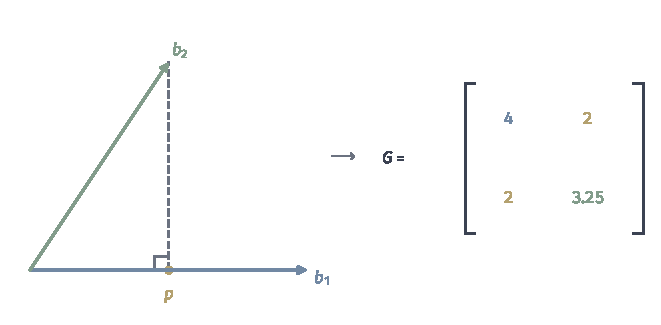
\includegraphics[width=112mm]{figures/00-shared/mathematical-preliminaries-upper/02-linear-spaces/matplotlib/ls-gram-matrix-coefficients/ls-gram-matrix-coefficients.pdf}
  \caption{Gram矩阵把一组基向量的两两内积排成数表。左：平面上两条不垂直的基向量$\bm b_1,\bm b_2$及其夹角；右：$G_{i,j}=\langle\bm b_i,\bm b_j\rangle$构成的$2\times2$Gram矩阵，对角元为各向量长度的平方，非对角元为两向量的内积。基越接近正交，非对角元越接近零；两向量共线时，某个非零组合的平方长度为零，Gram矩阵不再正定。向量与矩阵均为解析教学例。}
  \label{fig:ls-gram-matrix-coefficients}
\end{figure}

\subsection{Gram矩阵与半正定矩阵}
\label{sec:ls-gram-semidefinite}

\paragraph{Gram矩阵的半正定性}
Gram矩阵的二次型就是线性组合的长度平方。对任意系数向量$\bm a\in\mathbb R^r$，按双线性展开得
\[
 \bm a^\top\bm G\bm a=\sum_{i,j}a_ia_j\langle\bm b_i,\bm b_j\rangle=\Bigl\lVert\sum_j a_j\bm b_j\Bigr\rVert^2\geq0,
\]
所以Gram矩阵半正定。

Gram矩阵正定，当且仅当只有全零系数使线性组合$\sum_ja_j\bm b_j$为零，即这组向量线性无关（第~\ref{sec:ls-linear-dependence}节）：组合为零时平方长度为零，组合非零时平方长度为正。正定的Gram矩阵可逆：若$\bm G\bm a=\bm0$，则$\bm a^\top\bm G\bm a=0$，从而$\bm a=\bm0$，零空间为零（第~\ref{sec:ls-injective-surjective-invertible}节）。

近共线在Gram矩阵上也有对应的表现。
\begin{example}[近共线两列的Gram矩阵]
\label{ex:ls-nearly-collinear-gram}
仍取贯穿例的两列$\bm c_1,\bm c_2$与欧氏内积。示例~\ref{ex:ls-nearly-collinear-angle}已经算出三个内积，把它们排成矩阵，再写出二次型：
\[
\begin{gathered}
\bm G=\bm X_\varepsilon^\top\bm X_\varepsilon=\begin{bmatrix}3&3\\3&3+2\varepsilon^2\end{bmatrix},\\
\bm a^\top\bm G\bm a=3(a_1+a_2)^2+2\varepsilon^2a_2^2 .
\end{gathered}
\]
$\varepsilon\neq0$时，二次型只在$a_1=a_2=0$时为零，所以$\bm G$正定，这与两列线性无关一致。但正定的余量很小：取$\bm a=(1,-1)^\top$，第一个平方项消失，二次型只剩$2\varepsilon^2$；对应的组合$\bm c_1-\bm c_2=-\varepsilon\bm q$确实很短。近共线在Gram矩阵上的表现就是“正定但几乎退化”：系数不全为零，线性组合的长度平方却可以接近零。
\end{example}

\paragraph{Gram因子定理}
Gram矩阵总是半正定的。反过来，每个半正定矩阵是否都是某组向量的Gram矩阵？关键是把半正定矩阵的二次型写成欧氏平方和。下面的定理用逐步配方给出这一分解。
\begin{theorem}[半正定矩阵的配方因子]
\label{thm:ls-gram-factor}
设$\bm M\in\mathbb R^{r\times r}$对称半正定，则存在$\bm L\in\mathbb R^{r\times r}$使$\bm M=\bm L^\top\bm L$；若$\bm M$正定，可取$\bm L$可逆。
\end{theorem}
\begin{proof}
对$r$归纳。$r=1$时$\bm M=(m_{1,1})$且$m_{1,1}\geq0$，取$\bm L=(\sqrt{m_{1,1}})$即可。

设$r>1$。若所有对角元都为零，任取$i\neq j$，把$\bm x=\bm e_i+t\bm e_j$代入半正定性：
\[
 0\leq\bm x^\top\bm M\bm x=m_{i,i}+2t\,m_{i,j}+t^2m_{j,j}=2t\,m_{i,j}.
\]
这对正负$t$同时成立，迫使$m_{i,j}=0$，于是$\bm M=\bm0$，取$\bm L=\bm0$。

否则存在正的对角元。取一个置换矩阵$\bm P$把它换到首位（行列同步交换）；$\bm P$的各列是互不相同的标准坐标向量，所以$\bm P^\top\bm P=\bm P\bm P^\top=\bm I$。记
\[
\begin{gathered}
\widetilde{\bm M}=\bm P\bm M\bm P^\top
 =\begin{bmatrix}a&\bm b^\top\\ \bm b&\bm C\end{bmatrix},\\
a>0.
\end{gathered}
\]
$\widetilde{\bm M}$仍对称半正定，因为$\bm x^\top\widetilde{\bm M}\bm x=(\bm P^\top\bm x)^\top\bm M(\bm P^\top\bm x)\geq0$。对第一个变量配方：令$\bm x=(-\bm b^\top\bm u/a,\bm u)$，展开得$\bm x^\top\widetilde{\bm M}\bm x=\bm u^\top(\bm C-\bm b\bm b^\top/a)\bm u\geq0$，故余项$\bm M'=\bm C-\bm b\bm b^\top/a$仍半正定。由归纳假设$\bm M'=\bm L'^\top\bm L'$，取上三角因子
\[
 \widetilde{\bm L}=\begin{bmatrix}\sqrt a&\bm b^\top/\sqrt a\\ \bm0&\bm L'\end{bmatrix},
\]
按分块乘法直接相乘得
\[
 \widetilde{\bm L}^\top\widetilde{\bm L}
 =\begin{bmatrix}a&\bm b^\top\\ \bm b&\bm b\bm b^\top/a+\bm L'^\top\bm L'\end{bmatrix}
 =\widetilde{\bm M}.
\]
换回原矩阵：$\bm M=\bm P^\top\widetilde{\bm M}\bm P=(\widetilde{\bm L}\bm P)^\top(\widetilde{\bm L}\bm P)$，取$\bm L=\widetilde{\bm L}\bm P$即可。

正定时，$\bm M'$也正定（上述$\bm x$在$\bm u\neq\bm0$时非零），由归纳假设$\bm L'$可逆。分块上三角矩阵$\widetilde{\bm L}$的对角块$\sqrt a$与$\bm L'$都可逆，按分块乘法可以直接验证
\[
 \begin{bmatrix}1/\sqrt a&-\bm b^\top\bm L'^{-1}/a\\ \bm0&\bm L'^{-1}\end{bmatrix}
\]
是它的逆。于是$\bm L=\widetilde{\bm L}\bm P$作为可逆矩阵的乘积仍可逆。
\end{proof}
下面对一个二阶正定矩阵按证明的步骤求出因子。
\begin{example}[二阶正定矩阵的配方因子]
\label{ex:ls-gram-factor-two-by-two}
取示例~\ref{ex:ls-pd-psd-completing-square}中的正定矩阵
\[
 \bm M=\begin{bmatrix}4&2\\2&2\end{bmatrix}.
\]
首个对角元$a=4>0$，不需要置换。分块后$\bm b=(2)$，配方剩下的余项是$\bm M'=2-2^2/4=1$，它是一阶矩阵，取$\bm L'=(1)$。代入证明中的分块形式，
\[
 \bm L=\begin{bmatrix}\sqrt a&\bm b^\top/\sqrt a\\ 0&\bm L'\end{bmatrix}=\begin{bmatrix}2&1\\0&1\end{bmatrix}.
\]
相乘即可验证：
\[
 \bm L^\top\bm L=\begin{bmatrix}2&0\\1&1\end{bmatrix}\begin{bmatrix}2&1\\0&1\end{bmatrix}=\begin{bmatrix}4&2\\2&2\end{bmatrix}=\bm M.
\]
$\bm L$是对角元为正的上三角矩阵，因而可逆。它的两行正是配方中两个平方项的系数：
\[
 \bm x^\top\bm M\bm x=4x_1^2+4x_1x_2+2x_2^2=(2x_1+x_2)^2+x_2^2 ,
\]
即$\bm x^\top\bm M\bm x=\lVert\bm L\bm x\rVert_2^2$。证明中的分块步骤与手工配方是同一件事。
\end{example}
由这个分解，正定矩阵给出的加权长度可写成$\lVert\bm x\rVert_{\bm M}=\lVert\bm L\bm x\rVert_2$：加权内积就是把$\bm x$换成新坐标$\bm L\bm x$后再量欧氏长度。证明中的配方步骤就是第~\ref{sec:ls-cholesky}节Cholesky分解的雏形。

\paragraph{半正定矩阵是Gram矩阵}
因子定理回答了上面的问题：每个半正定矩阵都是某组向量的Gram矩阵。由定理~\ref{thm:ls-gram-factor}，半正定的$\bm M$可写成$\bm M=\bm L^\top\bm L$。记$\bm l_i$为$\bm L$的第$i$列，则$m_{i,j}=\bm l_i^\top\bm l_j=\langle\bm l_i,\bm l_j\rangle$，所以$\bm M$正是$\bm l_1,\ldots,\bm l_r$在欧氏内积下的Gram矩阵。于是“半正定”与“是一组向量的两两内积”说的是同一件事；要判断一个矩阵半正定，可以去找这样一组向量。

\subsection{Gram矩阵的逐元素乘法}
\label{sec:ls-schur-product}
利用“半正定矩阵就是Gram矩阵”这一刻画，可以判断两个半正定矩阵的逐元素乘积（第~\ref{sec:ls-hadamard-product}节）是否仍然半正定。

两个半正定矩阵分别是两组向量的Gram矩阵；只要再找到一组向量，使它们的两两内积恰为两个Gram矩阵对应元素之积，就能断定乘积半正定。所得结论称为\term{Schur乘积}定理（Schur product theorem）。
\begin{theorem}[Schur乘积定理]
\label{thm:ls-schur-product}
设$\bm A,\bm B$均为$n$阶对称半正定矩阵，则逐元素乘积$\bm A\odot\bm B$也对称半正定。
\end{theorem}
\begin{proof}
对称性由$(\bm A\odot\bm B)_{k,i}=A_{k,i}B_{k,i}=A_{i,k}B_{i,k}$直接得到。由定理~\ref{thm:ls-gram-factor}，$\bm A=\bm U^\top\bm U$、$\bm B=\bm V^\top\bm V$；记$\bm u_i,\bm v_i$分别为$\bm U,\bm V$的第$i$列，则$A_{i,k}=\langle\bm u_i,\bm u_k\rangle$、$B_{i,k}=\langle\bm v_i,\bm v_k\rangle$。考虑二阶数组$\bm u_1\otimes\bm v_1,\ldots,\bm u_n\otimes\bm v_n$。由Frobenius内积下张量积配对的分离性（第~\ref{sec:ls-tensor-product-properties}节），它们的Gram矩阵为
\[
 \langle\bm u_i\otimes\bm v_i,\bm u_k\otimes\bm v_k\rangle_{\mathrm F}
 =\langle\bm u_i,\bm u_k\rangle\langle\bm v_i,\bm v_k\rangle
 =A_{i,k}B_{i,k}.
\]
所以$\bm A\odot\bm B$是$\bm u_1\otimes\bm v_1,\ldots,\bm u_n\otimes\bm v_n$的Gram矩阵；Gram矩阵恒半正定，故$\bm A\odot\bm B$半正定。
\end{proof}
下面用一个二阶例子核对。
\begin{example}[两个半正定矩阵的逐元素乘积]
\label{ex:ls-schur-product}
取
\[
 \bm A=\bm B=\begin{bmatrix}1&1\\1&2\end{bmatrix}.
\]
先确认前提：$\bm A$的二次型为$x_1^2+2x_1x_2+2x_2^2=(x_1+x_2)^2+x_2^2\geq0$，所以$\bm A$半正定。逐元素相乘只把对角元$2$变成$4$，乘积及其二次型为
\[
\begin{gathered}
\bm A\odot\bm B=\begin{bmatrix}1&1\\1&4\end{bmatrix},\\
x_1^2+2x_1x_2+4x_2^2=(x_1+x_2)^2+3x_2^2\geq0 .
\end{gathered}
\]
配方后仍是平方和，$\bm A\odot\bm B$半正定，与定理~\ref{thm:ls-schur-product}一致。这里的配方只是核对；定理的作用在于，不必对每个乘积重新配方，就能断定结果半正定。
\end{example}
核方法中，两个核矩阵的逐元素乘积仍是合法的核矩阵，依据就是这一定理。

\subsection{基的Gram矩阵}
\label{sec:ls-gram-coordinates}

选定基以后，一般内积空间上的内积由基的Gram矩阵完全确定。设$\mathcal B=(\bm b_1,\ldots,\bm b_d)$是$V$的基，$\bm G$是它的Gram矩阵。对$\bm v=\sum_ix_i\bm b_i$、$\bm w=\sum_jy_j\bm b_j$，按双线性展开得
\[
 \langle\bm v,\bm w\rangle=\sum_{i,j}x_iy_j\langle\bm b_i,\bm b_j\rangle=[\bm v]_{\mathcal B}^\top\,\bm G\,[\bm w]_{\mathcal B}.
\]
基线性无关，由第~\ref{sec:ls-gram-semidefinite}节，$\bm G$对称正定。

因此在坐标下，任一内积都是以$\bm G$为权重的加权内积。特别地，$\mathbb R^d$上的任一内积在标准基下都是$\bm x^\top\bm G\bm y$，其中$g_{i,j}=\langle\bm e_i,\bm e_j\rangle$。

反过来，每个对称正定矩阵都给出一个加权内积。所以$\mathbb R^d$上的内积与$d$阶对称正定矩阵一一对应，欧氏内积对应$\bm I$。下面用示例~\ref{ex:ls-two-point-inner-product}的内积核对坐标公式。
\begin{example}[两点内积的坐标计算]
\label{ex:ls-two-point-inner-product-coordinates}
回到$P_1$上的内积$\langle f,g\rangle=f(0)g(0)+f(1)g(1)$，取基$(1,t)$，用两种方法计算$f=1+t$与$g=1-2t$的内积。坐标公式先要基的Gram矩阵。由$\langle1,1\rangle=1\cdot1+1\cdot1=2$、$\langle1,t\rangle=1\cdot0+1\cdot1=1$、$\langle t,t\rangle=0\cdot0+1\cdot1=1$，得
\[
 \bm G=\begin{bmatrix}2&1\\1&1\end{bmatrix}.
\]
直接按定义，$f$在$t=0,1$处取值$1,2$，$g$取值$1,-1$，所以$\langle f,g\rangle=1\cdot1+2\cdot(-1)=-1$。改用坐标，$[f]=(1,1)^\top$、$[g]=(1,-2)^\top$，
\[
 (1,1)\,\bm G\begin{bmatrix}1\\-2\end{bmatrix}=(3,2)\begin{bmatrix}1\\-2\end{bmatrix}=-1 .
\]
两种算法给出同一个值$-1$。由于$\bm G\neq\bm I$，坐标公式中的$\bm G$不能省去：本例中系数向量的欧氏内积碰巧也是$-1$，但示例~\ref{ex:ls-two-point-inner-product}中$\langle1,t\rangle=1$，系数向量的欧氏内积却是$0$。
\end{example}
若基两两正交且长度为$1$，则$\bm G=\bm I$，内积在坐标下就是欧氏内积；这样的基在第~\ref{sec:ls-orthonormal-bases}节讨论。

\paragraph{合同变换} 
换基时，Gram矩阵按另一种规则变化。若旧坐标与新坐标满足$\bm x=\bm C\widetilde{\bm x}$，内积中的两个坐标都要改变，因此Gram矩阵变为
\[
 \widetilde{\bm G}=\bm C^\top\bm G\bm C.
\]
这称为合同变换，它保持同一个内积与二次型。相似变换记录的则是同一个算子的换基，两者用途不同。

\subsection{复空间中的Gram矩阵}
\label{sec:ls-complex-gram}

前面的Gram矩阵都在实内积空间中讨论。按第~\ref{sec:ls-inner-product-axioms}节的约定，复内积对第一个变量共轭线性、对第二个变量线性，并满足$\langle\bm x,\bm y\rangle=\overline{\langle\bm y,\bm x\rangle}$。对复内积空间中的向量$\bm b_1,\ldots,\bm b_k$，Gram矩阵仍定义为$G_{i,j}=\langle\bm b_i,\bm b_j\rangle$。下面说明哪些结论照样成立，哪些需要修改。

\paragraph{自共轭代替对称}
实空间中，内积的对称性使Gram矩阵对称。复空间中，交换两个变量要取共轭：
\[
 G_{j,i}=\langle\bm b_j,\bm b_i\rangle=\overline{\langle\bm b_i,\bm b_j\rangle}=\overline{G_{i,j}},
\]
即$\bm G^*=\bm G$，其中$\bm G^*$是共轭转置。满足$\bm G^*=\bm G$的矩阵称为\term{自共轭矩阵}（Hermitian matrix），第~\ref{sec:ls-adjoints}节从伴随的角度称它为自伴矩阵。它的对角元$G_{i,i}=\lVert\bm b_i\rVert^2$是实数，非对角元一般是复数；$\bm G$一般不对称，$\bm G^\top=\overline{\bm G}$。实Gram矩阵是自共轭矩阵的特例，因为实矩阵的共轭转置就是转置。

\paragraph{半正定性照样成立}
对复系数向量$\bm c\in\mathbb C^k$，由内积对第一个变量共轭线性、对第二个变量线性，
\[
 \bm c^*\bm G\bm c=\sum_{i,j}\overline{c_i}\,c_j\langle\bm b_i,\bm b_j\rangle
 =\Bigl\langle\sum_ic_i\bm b_i,\sum_jc_j\bm b_j\Bigr\rangle
 =\Bigl\lVert\sum_jc_j\bm b_j\Bigr\rVert^2\geq0 .
\]
这与实情形的等式完全相同，只是左端的转置换成了共轭转置。自共轭矩阵的$\bm c^*\bm G\bm c$总是实数，所以“非负”有意义；称满足$\bm c^*\bm G\bm c\geq0$的自共轭矩阵为半正定。于是复Gram矩阵总是半正定的。

\paragraph{正定与线性无关的关系照样成立}
由同一等式，$\bm c^*\bm G\bm c=0$当且仅当$\sum_jc_j\bm b_j=\bm0$。所以$\bm G$正定，即$\bm c\neq\bm0$时$\bm c^*\bm G\bm c>0$，当且仅当$\bm b_1,\ldots,\bm b_k$在复数域上线性无关。这里的线性无关允许复系数：在实数域上无关的一组向量，在复数域上可能相关。例如在$\mathbb C$中，$1$与$\mathrm i$在实系数下无关，但$\mathrm i\cdot1-\mathrm i=0$，在复系数下相关；对应的Gram矩阵$\begin{bmatrix}1&\mathrm i\\-\mathrm i&1\end{bmatrix}$的行列式为$1-1=0$，确实不是正定的。

逐步配方的证明也保留。分块
\[
 \bm G=\begin{bmatrix}a&\bm b^*\\\bm b&\bm C\end{bmatrix}
\]
且$a>0$时，分离出的平方项为$a|z+\bm b^*\bm y/a|^2$，剩余矩阵是$\bm C-\bm b\bm b^*/a$；若对角元全为零，取只有两个分量非零且相位可调的向量，半正定性迫使所有非对角元也为零。递推便得到$\bm G=\bm L^*\bm L$：每个半正定的自共轭矩阵都是某组向量的Gram矩阵，不需要借用后面的谱定理。

\paragraph{坐标下的内积与换基}
在一组基下，复内积写成$\langle\bm x,\bm y\rangle=\bm x^*\bm G\bm y$，其中$\bm x,\bm y$表示坐标，$\bm G$是基的Gram矩阵，它是正定的自共轭矩阵。换基$\bm x=\bm C\widetilde{\bm x}$时，两个坐标都要改变，Gram矩阵变为$\bm C^*\bm G\bm C$，合同变换中的转置相应换成共轭转置。
\begin{example}[复空间中的Gram矩阵]
\label{ex:ls-complex-gram}
在$\mathbb C^2$上取标准内积$\langle\bm x,\bm y\rangle=\bm x^*\bm y$，计算$\bm b_1=(1,\mathrm i)^\top$与$\bm b_2=(1,1)^\top$的Gram矩阵。第一个变量要取共轭：$\langle\bm b_1,\bm b_1\rangle=1+|\mathrm i|^2=2$，$\langle\bm b_2,\bm b_2\rangle=2$，$\langle\bm b_1,\bm b_2\rangle=\overline1\cdot1+\overline{\mathrm i}\cdot1=1-\mathrm i$，$\langle\bm b_2,\bm b_1\rangle=1+\mathrm i$，所以
\[
 \bm G=\begin{bmatrix}2&1-\mathrm i\\1+\mathrm i&2\end{bmatrix}.
\]
两个非对角元互为共轭，所以$\bm G$不对称，但$\bm G^*=\bm G$。再看正定性。$\bm b_1,\bm b_2$在复数域上线性无关：若$\bm b_1=c\bm b_2$，比较两个坐标得$c=1$且$c=\mathrm i$，矛盾。由上面的结论，$\bm G$正定。在一个具体方向上核对：取$\bm c=(1,-1)^\top$，$\bm c^*\bm G\bm c=2-(1-\mathrm i)-(1+\mathrm i)+2=2=\lVert\bm b_1-\bm b_2\rVert^2>0$，两个虚部相互抵消，结果是实数。

这个例子显示了复情形改变的和保留的部分：Gram矩阵从对称变为自共轭，而半正定性以及正定与线性无关的对应，都与实情形相同。
\end{example}

% 内积空间：正交与投影（正交补、标准正交基、Gram--Schmidt正交化与QR分解、正交投影）。

\section{正交与投影}
\label{sec:ls-orthogonality-and-projection}

内积给出了两个向量之间的正交关系。本节把它推广到向量与子空间之间，把向量分解为子空间中的分量与和子空间正交的剩余部分。接着引入标准正交基，并用Gram--Schmidt正交化构造它；最后用标准正交基写出正交投影，证明它给出唯一的最近点。

\subsection{正交补与正交分解}
\label{sec:ls-orthogonality}

Gram矩阵记录的是一组向量两两之间是否正交。本小节考虑一个向量与整个子空间的正交，由此得到一个由内积唯一确定的补空间，并用它证明四个基本子空间之间的垂直关系。

\paragraph{正交补}
第~\ref{sec:ls-direct-sum}节说明，一个子空间的补空间一般不唯一。有了内积，可以挑出一个由垂直关系确定的补空间。设$U$是有限维内积空间$V$的子空间，与$U$中每个向量都正交的向量组成集合
\[
 U^\perp=\{\bm r\in V:\langle\bm u,\bm r\rangle=0,\ \forall\bm u\in U\},
\]
称为$U$的\term{正交补}（orthogonal complement）。由内积的双线性，$U^\perp$对线性组合封闭，是子空间。要检查$\bm r\in U^\perp$，只需检查它与$U$的一组基逐个正交，因为与基向量都正交的向量，也与基向量的每个组合正交。

\paragraph{正交直和}
下面证明正交补确实是一个补空间，而且分解可以由Gram矩阵算出。
\begin{lemma}[正交直和]
\label{lem:ls-orthogonal-decomposition}
设$U$是有限维内积空间$V$的子空间，则每个$\bm x\in V$唯一分解为$\bm x=\bm u+\bm r$，其中$\bm u\in U$、$\bm r\in U^\perp$；即$V=U\oplus U^\perp$。
\end{lemma}
\begin{proof}
取$U$的一组基$\bm b_1,\ldots,\bm b_r$。它线性无关，所以Gram矩阵$\bm G$正定，从而可逆。对任意$\bm x$，令$\bm u=\sum_j a_j\bm b_j$，并要求$\bm r=\bm x-\bm u$与每个$\bm b_i$正交，得到系数方程
\[
 \sum_j g_{i,j}a_j=\langle\bm b_i,\bm x\rangle\qquad(i=1,\ldots,r),
\]
写成矩阵形式就是Gram方程
\begin{equation}
 \bm G\bm a=(\langle\bm b_i,\bm x\rangle)_i .
 \label{eq:ls-gram-equation}
\end{equation}
$\bm G$可逆，所以系数唯一解出；残差$\bm r$与全部基向量正交，因而落在$U^\perp$。

若$\bm x=\bm u+\bm r=\bm u'+\bm r'$是两种分解，则$\bm u-\bm u'=\bm r'-\bm r$同时属于$U$与$U^\perp$。它与自身正交，长度为零，故两种分解相同。
\end{proof}
所以正交补是$U$的一个补空间，并且由内积唯一确定；$V=U\oplus U^\perp$称为正交直和。由维数公式，$\dim U^\perp=\dim V-\dim U$。下面在$\mathbb R^3$中做一次分解。
\begin{example}[向一条直线的正交分解]
\label{ex:ls-orthogonal-decomposition-line}
在$\mathbb R^3$中取欧氏内积，把$\bm y=(1,1.1,0.9)^\top$分解到直线$U=\operatorname{span}\{\bm c_1\}$及其正交补上，其中$\bm c_1=(1,1,1)^\top$。与$\bm c_1$正交就是坐标和为零，所以$U^\perp$是坐标和为零的平面。

$U$只有一个基向量，Gram方程只有一个未知数：
\[
 \langle\bm c_1,\bm c_1\rangle a=\langle\bm c_1,\bm y\rangle,\qquad\text{即}\ 3a=3,
\]
所以$a=1$。于是
\[
 \begin{gathered}
 \bm u=\bm c_1=(1,1,1)^\top,
 \\
 \bm r=\bm y-\bm u=(0,0.1,-0.1)^\top,
 \end{gathered}
\]
$\bm r$的坐标和为零，确实属于$U^\perp$。

所以$\bm y=\bm u+\bm r$就是$\bm y$在正交直和$\mathbb R^3=U\oplus U^\perp$中的分解：沿$\bm c_1$方向的部分是三个坐标的公共水平$1$，剩下的$(0,0.1,-0.1)^\top$记录各坐标偏离这个水平的程度。
\end{example}
这里只得到了正交分量的存在与唯一。它为什么是$U$中离$\bm y$最近的点，将在第~\ref{sec:ls-orthogonal-projection}节用标准正交基证明。

取两次正交补会回到原来的子空间：$(U^\perp)^\perp=U$。一方面，$U$中每个向量与$U^\perp$中每个向量正交，所以$U\subseteq(U^\perp)^\perp$。另一方面，对$U^\perp$用上面的维数关系，
\[
 \dim(U^\perp)^\perp=\dim V-\dim U^\perp=\dim U .
\]
二者包含且同维，由第~\ref{sec:ls-dimension}节，两者相等。

\paragraph{四个基本子空间的正交关系}
示例~\ref{ex:ls-rank-one-four-subspaces}显示，行空间的方向与零空间垂直，列空间的方向与左零空间垂直。现在在$\mathbb R^d$与$\mathbb R^m$上取欧氏内积，证明这对任何矩阵都成立。
\begin{theorem}[四个基本子空间的正交关系]
\label{thm:ls-four-subspaces-orthogonality}
设$\bm A\in\mathbb R^{m\times d}$，$\mathbb R^d$与$\mathbb R^m$取欧氏内积。则
\begin{equation}
\begin{gathered}
\operatorname{null}(\bm A)=\operatorname{range}(\bm A^\top)^\perp,\\
\operatorname{null}(\bm A^\top)=\operatorname{range}(\bm A)^\perp,
\end{gathered}
\label{eq:ls-four-subspaces-orthogonality}
\end{equation}
因而有正交直和
\begin{equation}
\begin{gathered}
\mathbb R^d=\operatorname{range}(\bm A^\top)\oplus\operatorname{null}(\bm A),\\
\mathbb R^m=\operatorname{range}(\bm A)\oplus\operatorname{null}(\bm A^\top).
\end{gathered}
\label{eq:ls-four-subspaces-decomposition}
\end{equation}
\end{theorem}
\begin{proof}
由转置的乘积规则（第~\ref{sec:ls-reshaping}节），对任意$\bm x\in\mathbb R^d$、$\bm y\in\mathbb R^m$，
\[
 \langle\bm A\bm x,\bm y\rangle=(\bm A\bm x)^\top\bm y=\bm x^\top(\bm A^\top\bm y)=\langle\bm x,\bm A^\top\bm y\rangle.
\]
$\bm y\in\operatorname{range}(\bm A)^\perp$意味着左端对一切$\bm x$为零，即右端对一切$\bm x$为零；取$\bm x=\bm A^\top\bm y$可见，这当且仅当$\bm A^\top\bm y=\bm0$。所以$\operatorname{range}(\bm A)^\perp=\operatorname{null}(\bm A^\top)$。

把$\bm A$换成$\bm A^\top$，得$\operatorname{range}(\bm A^\top)^\perp=\operatorname{null}(\bm A)$。正交直和由引理~\ref{lem:ls-orthogonal-decomposition}得到。
\end{proof}
两边再取正交补，并用$(U^\perp)^\perp=U$，还得到
\[
 \operatorname{null}(\bm A)^\perp=\operatorname{range}(\bm A^\top),\qquad
 \operatorname{null}(\bm A^\top)^\perp=\operatorname{range}(\bm A).
\]

于是输入空间分成两块互相垂直的部分：零空间是被$\bm A$消去的方向，行空间是真正影响输出的方向。输出空间也分成两块：列空间是能够到达的输出，左零空间中的方向则无论输入取什么都无法到达。

这一定理与第~\ref{sec:ls-kernel-image}节的维数关系相互印证。由正交直和与秩零度定理，分别得到
\[
 \begin{gathered}
d=\dim\operatorname{range}(\bm A^\top)+\dim\operatorname{null}(\bm A),\\
d=\operatorname{rank}\bm A+\dim\operatorname{null}(\bm A).
 \end{gathered}
\]
两式比较，又一次得到行秩等于列秩。示例~\ref{ex:ls-rank-one-four-subspaces}中逐项相乘再相加得零的观察，现在由定理得到了解释。

输出端的分解还给出方程$\bm A\bm x=\bm b$有解的一个判据：$\bm b\in\operatorname{range}(\bm A)$，当且仅当$\bm b$与左零空间中每个向量正交。第~\ref{chap:linear-solution-selection}章判断方程是否有解时会用到这一点。

\subsection{标准正交基}
\label{sec:ls-orthonormal-bases}

前面的计算都要用到Gram矩阵：正交分解要解Gram方程$\bm G\bm a=(\langle\bm b_i,\bm x\rangle)_i$，坐标下的内积要乘Gram矩阵。示例~\ref{ex:ls-coordinate-instability}还显示，接近共线的基会把小的对象记成很大的系数。这些麻烦都来自Gram矩阵的非对角元，即基向量之间的相互干扰。本小节研究Gram矩阵为单位矩阵的基：先证明它确实是一组基，再给出它下的坐标、对应的正交矩阵，以及这类基之间的换基。

\subsubsection{标准正交基的定义}
\label{sec:ls-orthonormal-basis-definition}
一组向量$\bm q_1,\ldots,\bm q_r$若满足
\[
 \langle\bm q_i,\bm q_j\rangle=\delta_{i,j}=\begin{cases}1,&i=j,\\0,&i\neq j,\end{cases}
\]
即两两正交且长度都为$1$，就称为标准正交组；它的Gram矩阵是$\bm I_r$。张成子空间$U$的标准正交组称为$U$的\term{标准正交基}（orthonormal basis）；$U=V$时就是$V$的标准正交基。

在$\mathbb R^m$中取欧氏内积，把$r$个向量排成$\bm Q\in\mathbb R^{m\times r}$的各列，它们的Gram矩阵是$\bm Q^\top\bm Q$，所以标准正交的条件就是$\bm Q^\top\bm Q=\bm I_r$。

$r=m$时，$\bm Q$是下面定义的正交矩阵。$r<m$时，$\bm Q^\top\bm Q=\bm I_r$仍成立，但$\bm Q\bm Q^\top$的秩只有$r$，不等于$\bm I_m$，$\bm Q$只有左逆$\bm Q^\top$。

\paragraph{标准正交组构成基}
标准正交组总是线性无关。设$\sum_jc_j\bm q_j=\bm0$，两边与$\bm q_i$作内积。左边每一项$c_j\langle\bm q_j,\bm q_i\rangle$只在$j=i$时不为零，于是$c_i=0$；$i$任意，所以全部系数为零。同样的论证说明两两正交的非零向量组线性无关，只是最后一步改为由$c_i\langle\bm q_i,\bm q_i\rangle=0$与$\langle\bm q_i,\bm q_i\rangle>0$得$c_i=0$。

因此标准正交组是它所张成子空间的一组基。在$d$维内积空间中，$d$个两两正交的单位向量的个数等于维数，自动构成整个空间的标准正交基，不必另行验证张成。

例如，$\mathbb R^d$的标准基在欧氏内积下是标准正交基；$\bm q_1=(1,1)^\top/\sqrt2$、$\bm q_2=(1,-1)^\top/\sqrt2$是$\mathbb R^2$的另一组标准正交基。

\subsubsection{标准正交基下的坐标}
\label{sec:ls-orthonormal-coordinates}
在标准正交基下，求坐标不必解方程，内积和长度也可以直接由坐标算出。
\begin{theorem}[Parseval恒等式]
\label{thm:ls-parseval}
设$\bm q_1,\ldots,\bm q_d$是实内积空间$V$的标准正交基。对任意$\bm v,\bm w\in V$，
\begin{equation}
 \bm v=\sum_{j=1}^d\langle\bm v,\bm q_j\rangle\,\bm q_j,
 \label{eq:ls-orthonormal-expansion}
\end{equation}
并且
\begin{equation}
 \langle\bm v,\bm w\rangle=\sum_{j=1}^d\langle\bm v,\bm q_j\rangle\langle\bm w,\bm q_j\rangle .
 \label{eq:ls-parseval-inner-product}
\end{equation}
特别地，
\begin{equation}
 \lVert\bm v\rVert^2=\sum_{j=1}^d\langle\bm v,\bm q_j\rangle^2.
 \label{eq:ls-parseval}
\end{equation}
\end{theorem}
\begin{proof}
设$\bm v=\sum_jc_j\bm q_j$。两边与$\bm q_i$作内积，由标准正交性，右边只剩$c_i$一项，所以$c_i=\langle\bm v,\bm q_i\rangle$，这就是式~\eqref{eq:ls-orthonormal-expansion}。再设$\bm w=\sum_jd_j\bm q_j$，由内积的双线性，
\[
 \langle\bm v,\bm w\rangle=\sum_{i,j}c_id_j\langle\bm q_i,\bm q_j\rangle=\sum_jc_jd_j,
\]
这就是第二式；取$\bm w=\bm v$即得式~\eqref{eq:ls-parseval}。
\end{proof}
式~\eqref{eq:ls-orthonormal-expansion}说明，每个系数只与自己的方向有关，增加或删去其他方向都不改变它。第二式说明，坐标下的内积就是坐标的欧氏内积。式~\eqref{eq:ls-parseval}称为Parseval恒等式：长度的平方等于各坐标的平方和，是勾股定理在$d$个互相垂直方向上的推广。下面用平面上的一组标准正交基验证这两点。
\begin{example}[标准正交基下的坐标与Parseval恒等式]
\label{ex:ls-orthonormal-coordinates}
取$\mathbb R^2$的标准正交基$\bm q_1=(1,1)^\top/\sqrt2$、$\bm q_2=(1,-1)^\top/\sqrt2$，求$\bm v=(3,1)^\top$的坐标。按式~\eqref{eq:ls-orthonormal-expansion}，每个坐标就是一次内积，不必解方程：
\[
 \langle\bm v,\bm q_1\rangle=\frac4{\sqrt2}=2\sqrt2,\qquad
 \langle\bm v,\bm q_2\rangle=\frac2{\sqrt2}=\sqrt2 .
\]

再核对Parseval恒等式：坐标的平方和与长度的平方分别为
\[
 (2\sqrt2)^2+(\sqrt2)^2=8+2=10,\qquad\lVert\bm v\rVert^2=3^2+1^2=10,
\]
两者相等。坐标换了，长度没有改变。
\end{example}
由Parseval恒等式，坐标的大小如实反映对象的大小，近共线基下“小对象、大系数”的现象不会发生。

\subsubsection{正交矩阵}
\label{sec:ls-orthogonal-matrices}
在$\mathbb R^n$中，以一组标准正交基为列的方阵有专门的名称。若$n$阶方阵$\bm Q$的各列都是单位向量，并且两两正交，就称它为\term{正交矩阵}（orthogonal matrix）。单位矩阵和置换矩阵都是正交矩阵，因为它们的列是互不相同的标准坐标向量。

下面检验平面旋转矩阵满足这一定义，并说明只有各列两两正交还不够。
\begin{example}[平面旋转是正交矩阵]
\label{ex:ls-rotation-orthogonal}
对任一实数$\phi$，平面旋转矩阵为
\[
 \bm R_\phi=\begin{bmatrix}\cos\phi&-\sin\phi\\\sin\phi&\cos\phi\end{bmatrix}.
\]
按定义逐列检验。两列的长度都是$\sqrt{\cos^2\phi+\sin^2\phi}=1$，两列的内积为
\[
 \cos\phi\cdot(-\sin\phi)+\sin\phi\cdot\cos\phi=0.
\]
所以$\bm R_\phi$是正交矩阵。

作为对照，对角矩阵$\operatorname{diag}(2,1)$的两列$(2,0)^\top$与$(0,1)^\top$内积为零，但第一列长度为$2$。它的各列两两正交，却不是正交矩阵：定义还要求每列长度为$1$。
\end{example}
逐列检验长度和内积比较繁琐。下面先把定义改写成一个矩阵等式，再由它推出正交矩阵的各项性质。

\paragraph{正交矩阵的转置条件}
$n$阶方阵$\bm Q$是正交矩阵，当且仅当
\begin{equation}
 \bm Q^\top\bm Q=\bm I_n.
 \label{eq:ls-orthogonal-matrix-condition}
\end{equation}
这是因为$(\bm Q^\top\bm Q)_{i,j}$是$\bm Q$的第$i$列与第$j$列的内积。“各列都是单位向量”对应对角元等于$1$，“各列两两正交”对应非对角元等于$0$，两者合起来正是这个矩阵等式。下面用这个条件重新检验示例~\ref{ex:ls-rotation-orthogonal}中的两个矩阵。
\begin{example}[用转置条件检验正交矩阵]
\label{ex:ls-orthogonality-by-transpose}
对旋转矩阵$\bm R_\phi$与对角矩阵$\operatorname{diag}(2,1)$，各算一次$\bm Q^\top\bm Q$：
\[
 \begin{aligned}
 \bm R_\phi^\top\bm R_\phi
 &=\begin{bmatrix}\cos\phi&\sin\phi\\-\sin\phi&\cos\phi\end{bmatrix}
   \begin{bmatrix}\cos\phi&-\sin\phi\\\sin\phi&\cos\phi\end{bmatrix}\\
 &=\begin{bmatrix}\cos^2\phi+\sin^2\phi&0\\0&\sin^2\phi+\cos^2\phi\end{bmatrix}
 =\bm I_2,\\
 \operatorname{diag}(2,1)^\top\operatorname{diag}(2,1)&=\operatorname{diag}(4,1)\neq\bm I_2.
 \end{aligned}
\]
$\bm R_\phi$满足转置条件，是正交矩阵。$\operatorname{diag}(2,1)$的乘积在$(1,1)$位置为$4\neq1$，正好对应第一列长度不为$1$；非对角元为零，对应两列正交。一次矩阵乘法同时完成了上例中逐列的全部检验。
\end{example}

\paragraph{正交矩阵保持内积}
由内积中的转置与转置条件，
\[
 \langle\bm Q\bm x,\bm Q\bm y\rangle=\langle\bm x,\bm Q^\top\bm Q\bm y\rangle=\langle\bm x,\bm y\rangle\qquad(\bm Q\text{为正交矩阵}).
\]
特别地，正交矩阵把两两正交的向量仍送到两两正交的向量。

\paragraph{正交矩阵的乘法}
若$\bm Q_1,\bm Q_2$是$n$阶正交矩阵，则
\[
 (\bm Q_1\bm Q_2)^\top(\bm Q_1\bm Q_2)=\bm Q_2^\top\bm Q_1^\top\bm Q_1\bm Q_2=\bm Q_2^\top\bm Q_2=\bm I_n,
\]
由转置条件，$\bm Q_1\bm Q_2$仍是正交矩阵。下面的例子显示，两个平面旋转的乘积不仅是正交矩阵，而且仍是旋转。
\begin{example}[两个平面旋转的乘积]
\label{ex:ls-rotation-composition}
把旋转矩阵$\bm R_\phi$与$\bm R_\psi$直接相乘，乘积的四个元素只由两个组合构成：
\[
 \bm R_\phi\bm R_\psi=\begin{bmatrix}c&-s\\s&c\end{bmatrix},
\]
其中
\[
 \begin{gathered}
 c=\cos\phi\cos\psi-\sin\phi\sin\psi,\\
 s=\sin\phi\cos\psi+\cos\phi\sin\psi.
 \end{gathered}
\]
由和角公式，$c=\cos(\phi+\psi)$，$s=\sin(\phi+\psi)$，所以
\[
 \bm R_\phi\bm R_\psi=\bm R_{\phi+\psi}.
\]
矩阵乘积$\bm R_\phi\bm R_\psi$先作用$\bm R_\psi$，所以这个等式说的是：先转$\psi$角、再转$\phi$角，等于一次转$\phi+\psi$角。乘积是正交矩阵，与上面的一般结论一致；这里还多知道一点，乘积仍是旋转。
\end{example}

\paragraph{正交矩阵的逆}
正交矩阵求逆只需转置：
\[
\begin{gathered}
\bm Q^{-1}=\bm Q^\top,\\
\bm Q\bm Q^\top=\bm I_n\qquad(\bm Q\text{为正交矩阵}).
\end{gathered}
\]
转置条件$\bm Q^\top\bm Q=\bm I_n$只说明$\bm Q^\top$是$\bm Q$的左逆。方阵只要有一侧的逆就可逆，而且这个单侧逆就是逆矩阵；这一点已在第~\ref{sec:ls-square-one-sided-inverse}节用行列式证明，第~\ref{sec:ls-injective-surjective-invertible}节又用核为零给出了另一个证明。由此$\bm Q^{-1}=\bm Q^\top$，另一侧的乘积$\bm Q\bm Q^\top$也等于$\bm I_n$。

$\bm Q\bm Q^\top$的$(i,j)$元是$\bm Q$的第$i$行与第$j$行的内积，所以正交矩阵的各行同样两两正交且长度为$1$。又因$(\bm Q^\top)^\top\bm Q^\top=\bm Q\bm Q^\top=\bm I_n$，由转置条件，$\bm Q^{-1}=\bm Q^\top$也是正交矩阵。

\paragraph{正交矩阵的行列式}
正交矩阵的行列式只能取两个值：
\[
 \det\bm Q=\pm1\qquad(\bm Q\text{为正交矩阵}).
\]
由行列式的乘积公式，
\[
 \det(\bm Q^\top)\det\bm Q=\det(\bm Q^\top\bm Q)=\det\bm I_n=1;
\]
再由$\det(\bm Q^\top)=\det\bm Q$，得$(\det\bm Q)^2=1$。

旋转$\bm R_\phi$的行列式为$\cos^2\phi+\sin^2\phi=1$；交换两个坐标的置换矩阵行列式为$-1$，它翻转了定向。

\subsubsection{标准正交基之间的换基}
\label{sec:ls-orthonormal-change-of-basis}
正交矩阵也出现在标准正交基之间的换基中。设$\mathcal B=(\bm b_1,\ldots,\bm b_d)$与$\mathcal C$都是$V$的标准正交基，换基矩阵$\bm S=\bm S_{\mathcal C\leftarrow\mathcal B}$的第$j$列是$\bm b_j$的$\mathcal C$坐标。在标准正交基$\mathcal C$下，内积就是坐标的欧氏内积，所以$\bm S$的第$i$、$j$两列的欧氏内积等于$\langle\bm b_i,\bm b_j\rangle=\delta_{i,j}$，即$\bm S^\top\bm S=\bm I$。因此两组标准正交基之间的换基矩阵是正交矩阵。

于是反向换基只需转置，$\bm S^{-1}=\bm S^\top$，不会出现示例~\ref{ex:ls-nearly-collinear-change-of-basis}中除以小数$\varepsilon$的放大。例如从上面的$(\bm q_1,\bm q_2)$换到标准基，换基矩阵的两列就是$\bm q_1,\bm q_2$本身。

对线性算子，若只在标准正交基之间换基，相似关系$\bm B=\bm P^{-1}\bm A\bm P$变成$\bm B=\bm P^\top\bm A\bm P$。第~\ref{chap:eigen-spectral-decomposition}章的谱定理就是在这种受限的换基下化简对称矩阵。

\paragraph{正交不变性}
正交矩阵保持欧氏长度，因此也不改变与欧氏长度相关的矩阵范数。设$\bm Q$为正交矩阵，则
\[
 \begin{gathered}
 \lVert\bm Q\bm x\rVert_2=\lVert\bm x\rVert_2,\\
 \lVert\bm Q\rVert_2=1,
 \end{gathered}
\]
\[
 \begin{gathered}
 \lVert\bm Q\bm A\rVert_{\mathrm F}=\lVert\bm A\rVert_{\mathrm F},\\
 \lVert\bm Q\bm A\rVert_2=\lVert\bm A\rVert_2.
 \end{gathered}
\]
先看向量。由转置条件，
\[
 \lVert\bm Q\bm x\rVert_2^2=\bm x^\top\bm Q^\top\bm Q\bm x=\lVert\bm x\rVert_2^2,
\]
正交矩阵保持欧氏长度，所以每个比值$\lVert\bm Q\bm x\rVert_2/\lVert\bm x\rVert_2$都等于$1$，$\lVert\bm Q\rVert_2=1$。

对矩阵$\bm A$，左乘$\bm Q$不改变各列的长度，$\lVert\bm Q\bm A_{:,j}\rVert_2=\lVert\bm A_{:,j}\rVert_2$，对$j$求平方和即得$\lVert\bm Q\bm A\rVert_{\mathrm F}=\lVert\bm A\rVert_{\mathrm F}$。

左乘$\bm Q$也不改变每个输出的长度，$\lVert\bm Q\bm A\bm x\rVert_2=\lVert\bm A\bm x\rVert_2$，取上确界即得$\lVert\bm Q\bm A\rVert_2=\lVert\bm A\rVert_2$。

\subsection{Gram--Schmidt正交化}
\label{sec:ls-orthonormal-basis-construction}

本小节说明，任意一组线性无关的向量都可以改造成标准正交组。思路来自正交分解：依次处理各向量，从每个向量中扣除它在已经得到的方向上的分量，剩下的部分与这些方向都垂直，再把它缩放到单位长度。下面先给出这一过程并证明它总能完成，再把它在$\mathbb R^m$中写成矩阵分解，最后处理各列线性相关的情形。

\subsubsection{Gram--Schmidt正交化}

这一过程称为\term{Gram--Schmidt正交化}（Gram--Schmidt orthogonalization），也称施密特正交化。设$\bm v_1,\ldots,\bm v_k$线性无关。令$\bm u_1=\bm v_1$、$\bm q_1=\bm u_1/\lVert\bm u_1\rVert$；对$j=2,\ldots,k$依次令
\begin{equation}
\begin{gathered}
\bm u_j=\bm v_j-\sum_{i=1}^{j-1}\langle\bm v_j,\bm q_i\rangle\bm q_i,\\
\bm q_j=\frac{\bm u_j}{\lVert\bm u_j\rVert}.
\end{gathered}
\label{eq:ls-gram-schmidt}
\end{equation}
扣除的部分在$\operatorname{span}\{\bm q_1,\ldots,\bm q_{j-1}\}$中，剩下的$\bm u_j$与这些方向都正交，所以$\bm u_j$正是正交分解中的剩余分量。下面的定理验证这一点，并说明过程不会中断。
\begin{theorem}[Gram--Schmidt正交化]
\label{thm:ls-gram-schmidt}
上述过程中每个$\bm u_j\neq\bm0$，得到的$\bm q_1,\ldots,\bm q_k$两两正交、长度为$1$，并且对每个$j$都有$\operatorname{span}\{\bm q_1,\ldots,\bm q_j\}=\operatorname{span}\{\bm v_1,\ldots,\bm v_j\}$。
\end{theorem}
\begin{proof}
对$j$归纳。$j=1$时$\bm u_1=\bm v_1\neq\bm0$，结论成立。设结论对$j-1$成立。对$i<j$，由$\bm q_1,\ldots,\bm q_{j-1}$两两正交且长度为$1$，
\[
 \langle\bm u_j,\bm q_i\rangle=\langle\bm v_j,\bm q_i\rangle-\langle\bm v_j,\bm q_i\rangle\langle\bm q_i,\bm q_i\rangle=0,
\]
所以$\bm u_j$与前面的方向都正交。

若$\bm u_j=\bm0$，则$\bm v_j$落在前$j-1$个新方向的张成空间中。由归纳假设，这也是前$j-1$个原向量的张成空间，与线性无关矛盾；故$\bm u_j\neq\bm0$，$\bm q_j$有定义且长度为$1$。

最后比较张成空间。$\bm q_j$是$\bm v_j$与$\bm q_1,\ldots,\bm q_{j-1}$的组合，因而属于$\operatorname{span}\{\bm v_1,\ldots,\bm v_j\}$。反过来，由式~\eqref{eq:ls-gram-schmidt}，
\[
 \bm v_j=\lVert\bm u_j\rVert\bm q_j+\sum_{i<j}\langle\bm v_j,\bm q_i\rangle\bm q_i
\]
属于$\operatorname{span}\{\bm q_1,\ldots,\bm q_j\}$。两个张成空间互相包含，因而相等。
\end{proof}
对有限维内积空间的任意一组基作Gram--Schmidt正交化，就得到一组标准正交基，所以\emph{每个有限维内积空间都有标准正交基}。若已有几个两两正交的单位向量，可以先把它们扩充成一组基，再从它们之后开始正交化。前面的向量在过程中保持不变，所以任何标准正交组都能扩充成标准正交基。

张成空间逐段相等也有用处：前$j$个新方向与前$j$个旧方向张成同一个子空间，正交化只是在每一段内部换了一组更好用的基。

\paragraph{算例}
标准正交基依赖内积；换一个内积，同一组基正交化的结果也不同。下面在示例~\ref{ex:ls-two-point-inner-product}的内积下对基$(1,t)$作正交化。在这个内积下$\langle1,t\rangle=1\neq0$，两个基向量并不正交。
\begin{example}[两点内积下的Gram--Schmidt正交化]
\label{ex:ls-gram-schmidt-two-point}
在$P_1$的内积$\langle f,g\rangle=f(0)g(0)+f(1)g(1)$下，对基$(1,t)$逐步执行式~\eqref{eq:ls-gram-schmidt}。这个内积只看$t=0,1$两处的取值，所以每次计算内积或长度，都先写出函数在这两点的值。

先归一化第一个基向量。常数$1$在两点都取$1$，$\lVert1\rVert^2=1^2+1^2=2$，所以
\[
 q_1=\frac1{\sqrt2}.
\]
再从$t$中扣除它在$q_1$上的分量。$t$在两点取值$0,1$，所以
\[
 \langle t,q_1\rangle=\frac{0\cdot1+1\cdot1}{\sqrt2}=\frac1{\sqrt2},
\]
扣除后得到
\[
 u_2=t-\langle t,q_1\rangle q_1=t-\frac1{\sqrt2}\cdot\frac1{\sqrt2}=t-\frac12.
\]
扣除的常数$\tfrac12$正是$t$在两点取值的平均。

最后归一化。$u_2$在$t=0,1$处的取值为$-\tfrac12,\tfrac12$，所以
\[
 \lVert u_2\rVert^2=\frac14+\frac14=\frac12,
\]
于是
\[
 q_2=\frac{u_2}{\lVert u_2\rVert}=\sqrt2\Bigl(t-\frac12\Bigr).
\]

可以核对结果确实标准正交。$q_1$在$t=0,1$处取值都是$\tfrac1{\sqrt2}$，$q_2$取值为$-\tfrac{\sqrt2}2,\tfrac{\sqrt2}2$，所以
\[
 \begin{gathered}
 \langle q_1,q_2\rangle=\frac1{\sqrt2}\cdot\Bigl(-\frac{\sqrt2}2\Bigr)+\frac1{\sqrt2}\cdot\frac{\sqrt2}2=0,\\
 \lVert q_2\rVert^2=\frac12+\frac12=1.
 \end{gathered}
\]

有了标准正交基，坐标就由内积直接读出。$f=1+t$在$t=0,1$处取值为$1,2$，所以
\[
 \begin{gathered}
 \langle f,q_1\rangle=\frac{1+2}{\sqrt2}=\frac3{\sqrt2},\\
 \langle f,q_2\rangle=1\cdot\Bigl(-\frac{\sqrt2}2\Bigr)+2\cdot\frac{\sqrt2}2=\frac{\sqrt2}2 .
 \end{gathered}
\]

用这两个坐标还原，得
\[
 \frac3{\sqrt2}\cdot\frac1{\sqrt2}+\frac{\sqrt2}2\cdot\sqrt2\Bigl(t-\frac12\Bigr)=\frac32+t-\frac12=1+t .
\]
Parseval恒等式也成立：$\lVert f\rVert^2=1^2+2^2=5$，而坐标的平方和为$\tfrac92+\tfrac12=5$。

所以$q_1=1/\sqrt2$、$q_2=\sqrt2(t-\tfrac12)$是这一内积下$P_1$的标准正交基，$1+t$在其下的坐标为$(3/\sqrt2,\ \sqrt2/2)$。
\end{example}
正交化把$t$换成了$t-\tfrac12$。在系数向量的欧氏内积下，$1$与$t$的系数列$(1,0)^\top$、$(0,1)^\top$本来就正交；换了内积以后，才需要这一步。

\subsubsection{QR分解}

在$\mathbb R^m$中取欧氏内积，Gram--Schmidt正交化可以写成一个矩阵等式。它把一组列向量的方向与组合系数分开记录。

设$\bm A\in\mathbb R^{m\times d}$的列$\bm a_1,\ldots,\bm a_d$线性无关，对它们作正交化，即取$\bm v_j=\bm a_j$。把式~\eqref{eq:ls-gram-schmidt}反过来写，得
\[
 \bm a_j=\lVert\bm u_j\rVert\bm q_j+\sum_{i<j}\langle\bm a_j,\bm q_i\rangle\bm q_i .
\]
所以每一列只用到前$j$个正交方向：
\[
 \bm a_j=\sum_{i\leq j}r_{i,j}\bm q_i,
\]
其中
\[
 r_{i,j}=\langle\bm a_j,\bm q_i\rangle\quad(i<j),\qquad
 r_{j,j}=\lVert\bm u_j\rVert>0 .
\]
把$\bm q_1,\ldots,\bm q_d$排成$\bm Q\in\mathbb R^{m\times d}$，把系数$r_{i,j}$排成$d$阶上三角矩阵$\bm R$（$i>j$时$r_{i,j}=0$）。按矩阵乘积的列读法，各列的这些关系合写为经济型\term{QR分解}（QR factorization）
\begin{equation}
 \begin{gathered}
 \bm A=\bm Q\bm R,\\
 \bm Q^\top\bm Q=\bm I_d,\qquad\bm R\text{ 上三角且对角元为正}.
 \end{gathered}
\label{eq:ls-qr-factorization}
\end{equation}
由定理~\ref{thm:ls-gram-schmidt}，$\bm Q$的列是列空间$\operatorname{range}(\bm A)$的标准正交基，$\bm R$的第$j$列记录$\bm a_j$在这组正交方向上的坐标。$\bm R$的对角元为正，所以$\bm R$可逆。

图~\ref{fig:vol1-add-linear-qr-columns}给出最小的二维情形：保留第一个单位方向，从第二列减去它在第一个方向上的分量，列空间不变，减去的部分记进$\bm R$。
\begin{figure}[!htb]
  \centering
  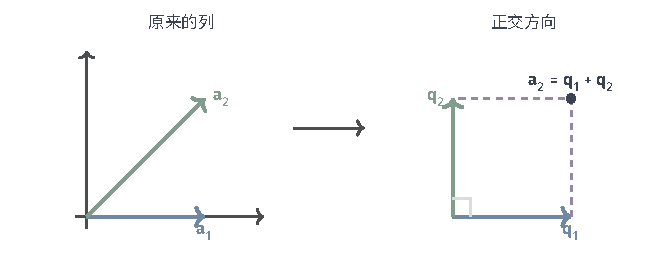
\includegraphics[width=112mm]{figures/00-shared/mathematical-preliminaries-upper/02-linear-spaces/tikz/comprehension-additions/linear-qr-columns.pdf}
  \caption{QR分解把列的方向和组合系数分开。取$\bm a_1=(1,0)^\top$、$\bm a_2=(1,1)^\top$，
  正交化得到$\bm q_1=(1,0)^\top$、$\bm q_2=(0,1)^\top$，并有$\bm a_1=\bm q_1$、
  $\bm a_2=\bm q_1+\bm q_2$，故$\bm R=\left[\begin{smallmatrix}1&1\\0&1\end{smallmatrix}\right]$。
  虚线补出第二列的分量。}
  \label{fig:vol1-add-linear-qr-columns}
\end{figure}

这一分解的用处在于，涉及列空间的计算可以改在标准正交的$\bm Q$上进行，坐标由内积直接读出，不必再解Gram方程。第~\ref{chap:linear-solution-selection}章与第~\ref{chap:direct-linear-solvers}章解方程与最小二乘问题时就是这样使用它的。

\subsubsection{列相关时的处理}

定理~\ref{thm:ls-gram-schmidt}要求各列线性无关。若不满足，某一步会出现$\bm u_j=\bm0$。由正交分解，这恰好说明$\bm a_j$已在前面方向张成的空间中，没有带来新方向。这时不能对零向量归一化，应跳过这一列，只在$\bm R$中记下它的系数$\langle\bm a_j,\bm q_i\rangle$。跳过它不影响后续各列，因为张成的空间没有变。

全部处理完以后，留下的$\bm q$的个数等于列空间的维数$r=\operatorname{rank}\bm A$，仍有$\bm A=\bm Q\bm R$。其中$\bm Q\in\mathbb R^{m\times r}$的列是列空间的标准正交基；$\bm R\in\mathbb R^{r\times d}$各行从左到右第一个非零元的位置逐行右移。$r<d$时$\bm R$不是方阵，不能求逆。下面是最小的例子。
\begin{example}[列相关时跳过零余量]
\label{ex:ls-qr-dependent-columns}
设$\bm A=[\bm a_1\ \bm a_2]$，其中$\bm a_1=(1,0)^\top$、$\bm a_2=(2,0)^\top$，第二列是第一列的两倍。$\bm a_1$已是单位向量，$\bm q_1=\bm a_1$。处理第二列时，$\langle\bm a_2,\bm q_1\rangle=2$，扣除后
\[
 \bm u_2=\bm a_2-2\bm q_1=\bm0,
\]
第二列没有带来新方向。于是跳过$\bm a_2$，只在$\bm R$中记下系数$2$，得到$r=1$，
\[
\begin{gathered}
\bm Q=\begin{bmatrix}1\\0\end{bmatrix},\\
\bm R=\begin{bmatrix}1&2\end{bmatrix},\\
\bm Q\bm R=\begin{bmatrix}1&2\\0&0\end{bmatrix}=\bm A .
\end{gathered}
\]
乘回去仍得到$\bm A$，说明跳过的列并没有丢失信息，它的系数保存在$\bm R$中。

列空间是$x$轴，$\bm Q$的唯一一列构成它的标准正交基，留下的列数$1$正是$\operatorname{rank}\bm A$；$\bm R$是$1\times2$矩阵，不能求逆。
\end{example}
于是在精确算术下，同一过程也给出列空间的一组标准正交基与矩阵的秩。有限精度下，扣除后的余量很少恰好为零；怎样判断它“算作零”，以及怎样改写扣除顺序以减少正交性的损失，属于数值计算问题，在第~\ref{sec:ls-numerical-sensitivity}节讨论。

\subsection{正交投影}
\label{sec:ls-orthogonal-projection}

标准正交基使子空间中的分量可以逐个读出。把这些分量合在一起，就得到正交投影。本小节证明它是子空间中离原向量最近的点，再把它写成矩阵，并给出判断一个矩阵是否为正交投影的方法。

\paragraph{向子空间的正交分解}
若$\bm q_1,\ldots,\bm q_r$是子空间$U$的标准正交基，引理~\ref{lem:ls-orthogonal-decomposition}中的Gram矩阵是单位矩阵，Gram方程直接给出$\bm a=(\langle\bm q_i,\bm x\rangle)_i$。于是分解可以直接写出：
\begin{equation}
 \bm x=\underbrace{\sum_{j=1}^r\langle\bm x,\bm q_j\rangle\bm q_j}_{\bm u\in U}+\underbrace{\Bigl(\bm x-\sum_{j=1}^r\langle\bm x,\bm q_j\rangle\bm q_j\Bigr)}_{\bm r\in U^\perp}.
 \label{eq:ls-orthonormal-projection}
\end{equation}
$\bm u$称为$\bm x$在$U$上的正交投影。$\bm u$与$\bm r$正交，由勾股定理，
\[
 \lVert\bm x\rVert^2=\lVert\bm u\rVert^2+\lVert\bm r\rVert^2\geq\sum_{j=1}^r\langle\bm x,\bm q_j\rangle^2.
\]
即沿一部分标准正交方向读出的系数，其平方和不超过总长度的平方；等号恰在$\bm x\in U$时成立。

$\bm u$正是子空间中离$\bm x$最近的点。
\begin{theorem}[正交投影是最近点]
\label{thm:ls-orthogonal-projection-nearest}
设$U$是内积空间$V$的有限维子空间，$\bm x\in V$，$\bm u$是$\bm x$在$U$上的正交投影。对任意$\bm v\in U$，
\[
 \lVert\bm x-\bm v\rVert^2=\lVert\bm x-\bm u\rVert^2+\lVert\bm u-\bm v\rVert^2,
\]
因此$\lVert\bm x-\bm v\rVert\geq\lVert\bm x-\bm u\rVert$，等号当且仅当$\bm v=\bm u$。也就是说，$\bm u$是$U$中唯一离$\bm x$最近的点。
\end{theorem}
\begin{proof}
$\bm x-\bm v=(\bm x-\bm u)+(\bm u-\bm v)$的两项分别属于$U^\perp$和$U$，彼此正交，由勾股定理即得等式。右端第二项非负，并且只在$\bm v=\bm u$时为零。
\end{proof}
基不是标准正交时，同样可以先解Gram方程求出投影；实际求解时不必显式形成逆矩阵。

最近点的唯一性来自内积确定的正交分解。第~\ref{sec:ls-quotient-norms}节已经证明一般范数下最近点存在，示例~\ref{ex:ls-linf-nonunique-nearest}却在$\ell_\infty$范数下给出了无穷多个最近点；同一个点在欧氏范数下的最近点只有原点，因为
\[
 \lVert\bm y-(t,0)^\top\rVert_2^2=t^2+1
\]
只在$t=0$时取最小值。

下面用标准正交基重算前面的正交分解。
\begin{example}[用标准正交基重算正交分解]
\label{ex:ls-orthonormal-projection-line}
回到示例~\ref{ex:ls-orthogonal-decomposition-line}的$\bm y=(1,1.1,0.9)^\top$与直线$U$，这次先把方向向量归一化为$\bm q_1=(1,1,1)^\top/\sqrt3$，于是$U=\operatorname{span}\{\bm q_1\}$。投影系数就是一次内积，由它得到投影与余量：
\[
 \begin{gathered}
 \langle\bm y,\bm q_1\rangle=\frac3{\sqrt3}=\sqrt3,\qquad
 \sqrt3\,\bm q_1=(1,1,1)^\top,\\
 \bm y-\sqrt3\,\bm q_1=(0,0.1,-0.1)^\top .
 \end{gathered}
\]
余量与$\bm q_1$正交。

结果与前例相同，但这里不需要解Gram方程：归一化已经把Gram矩阵变成了$1$。由上面的最近点性质，$(1,1,1)^\top$还是直线$U$上离$\bm y$最近的点。
\end{example}

\paragraph{投影矩阵}
\label{sec:ls-projection-matrices}
正交投影随原向量线性变化。记$\bm y$在$U$上的正交投影为$\bm p$。$\bm y_1,\bm y_2$的正交分解相加、数乘后仍是正交分解，由分解的唯一性，投影也随之相加、数乘。所以$\bm y\mapsto\bm p$是一个线性映射，称为到$U$的正交投影。

在欧氏内积下，它可以写成矩阵。设$\bm Q$的列是$U$的标准正交基。按矩阵乘积的列读法，
\[
 \bm p=\sum_j\langle\bm q_j,\bm y\rangle\bm q_j=\bm Q\bm Q^\top\bm y,
\]
所以到$U$的正交投影是
\begin{equation}
\begin{gathered}
\bm P_U=\bm Q\bm Q^\top,\\
\bm P_U^\top=\bm P_U,\\
\bm P_U^2=\bm P_U.
\end{gathered}
\label{eq:linear-algebra-orthogonal-projector}
\end{equation}
两条性质都可以直接验证。由$\bm Q^\top\bm Q=\bm I$，
\[
 \bm P_U^2=\bm Q(\bm Q^\top\bm Q)\bm Q^\top=\bm Q\bm Q^\top=\bm P_U,
\]
即幂等：已经在$U$中的点再投影一次不变。又$(\bm Q\bm Q^\top)^\top=\bm Q\bm Q^\top$，即对称：内积中可以把投影移到另一侧。

此外$\operatorname{range}\bm P_U=\operatorname{range}\bm Q=U$。$\bm Q$不是方阵时，$\bm P_U$通常不是单位矩阵，它只保留$U$中的分量。

\paragraph{正交投影、斜投影与幂等}
拿到一个矩阵，怎样判断它是不是正交投影？幂等性只说明它是某种投影，不说明它给出最近点。一般的幂等矩阵$\bm P$把$\bm y$分成$\bm P\bm y$与$\bm y-\bm P\bm y$两部分，前者在像中，后者在零空间中，因为$\bm P(\bm y-\bm P\bm y)=\bm P\bm y-\bm P^2\bm y=\bm0$。但两部分不必正交。这种映射称为\term{斜投影}（oblique projection）。

\begin{example}[反例：幂等而不对称的投影]
\label{ex:ls-oblique-projection}
取
\[
 \bm P=\begin{bmatrix}1&-1\\0&0\end{bmatrix}.
\]
直接相乘得$\bm P^2=\bm P$，所以它幂等；它把$(y_1,y_2)^\top$送到$x$轴上的$(y_1-y_2,0)^\top$。

残差$\bm y-\bm P\bm y=(y_2,y_2)^\top$与$x$轴方向$(1,0)^\top$的内积是$y_2$，$y_2\neq0$时不为零，所以$\bm P\bm y$不是$x$轴上离$\bm y$最近的点。这个$\bm P$也不对称：$\bm P^\top\neq\bm P$。
\end{example}

对称性正是正交的条件。若$\bm P$幂等且对称，对任意$\bm y,\bm z$有
\[
 (\bm y-\bm P\bm y)^\top\bm P\bm z=\bm y^\top(\bm P-\bm P^\top\bm P)\bm z=\bm y^\top(\bm P-\bm P^2)\bm z=0,
\]
即残差与整个像正交。于是$\bm y=\bm P\bm y+(\bm y-\bm P\bm y)$是$\bm y$关于像空间的正交分解，由分解的唯一性，$\bm P$就是到其像的正交投影。

所以判别分两步：先验幂等，判断是不是投影；再验对称，判断是不是正交投影。

\section{本章小结}
\label{sec:ls-inner-product-spaces-summary}

本章回答了章首的问题：内积在一般线性空间上规定了角度，由此可以判断垂直、求出最好的近似，并选出让坐标计算最简单的基。

内积给出长度、正交与夹角。Cauchy--Schwarz不等式保证夹角有定义；内积诱导的长度满足三角不等式，因而是范数，并给出距离。并非每个范数都来自内积，平行四边形恒等式可以检验这一点；有限维内积空间是Hilbert空间。

Gram矩阵记录一组向量的两两内积。它总是半正定的，并且恰在这组向量线性无关时正定；反过来，每个半正定矩阵都是某组向量的Gram矩阵，这又推出逐元素乘积保持半正定。基的Gram矩阵把一般内积写成坐标的计算公式，换基时按合同变换改变。

正交分解把向量拆成子空间中的部分与垂直的部分。标准正交基使坐标可以由内积直接读出，Parseval恒等式说明长度的平方等于坐标的平方和；正交矩阵是标准正交基之间的换基矩阵，求逆只需转置，并保持欧氏长度。Gram--Schmidt正交化保证标准正交基总存在，QR分解把这一过程写成矩阵形式。正交投影是子空间中唯一的最近点；矩阵是正交投影，当且仅当它幂等且对称。

这些结论为后续各章提供几何工具。第~\ref{chap:dual-spaces}章用内积把线性泛函表示为向量、把对偶映射改写为伴随；第~\ref{chap:eigen-spectral-decomposition}章在正交换基下寻找线性作用的简单表示，正交矩阵与自伴算子在那里尤为重要；最小二乘、QR求解与正交投影则贯穿线性方程各章。


\chapter{对偶空间}
\label{chap:dual-spaces}

线性映射把对象送到另一个空间。还有一类更简单的作用，只把对象读成一个数：取多项式在某一点的值，取信号的第一个样本，计算一组特征的加权和。第~\ref{sec:ls-coordinates}节的每个坐标$x_j$也是这样的读取。本章把这类线性读取本身当作研究对象，并回答三个问题：全部读取组成什么样的空间，读取怎样随线性映射在两端之间传递，以及一个读取有多大。

前两节只用线性运算。第~\ref{sec:ls-dual-space}节说明全部线性读取组成一个线性空间，即对偶空间，并用坐标读取构造它的基；第~\ref{sec:ls-dual-map}节研究对象经过线性映射以后，输出端的读取怎样传回输入端。这种传回在坐标下就是转置，它给第~\ref{chap:linear-operations}章“行列互换”的操作一个不依赖坐标的含义。

后三节加入度量结构。第~\ref{sec:ls-dual-norms}节借助第~\ref{chap:normed-spaces}章的范数度量读取的大小，即误差受限时读取的最大变化。第~\ref{sec:ls-riesz-representation}节借助第~\ref{chap:inner-product-spaces}章的内积，把每个读取写成与一个固定向量的内积；第~\ref{sec:ls-adjoints}节再把对偶映射改写成内积空间之间的映射，即伴随，并由伴随定义自伴、正交与正规算子。

本章依赖第~\ref{chap:linear-representation}章的基、坐标与线性映射，第~\ref{chap:normed-spaces}章的范数与诱导矩阵范数，以及第~\ref{chap:inner-product-spaces}章的内积、Gram矩阵与标准正交基。全章只讨论有限维空间；无限维空间中并非每个线性泛函都连续，那里的对偶理论属于函数空间。

% 对偶空间：线性泛函、对偶空间与对偶基。

\section{线性泛函}
\label{sec:ls-dual-space}
\phantomsection
\label{sec:ls-dual-spaces}

\paragraph{线性泛函的定义}
保持线性组合的标量读取称为\term{线性泛函}（linear functional），即满足
\[
\varphi(a\bm x+b\bm y)=a\varphi(\bm x)+b\varphi(\bm y),\qquad\bm x,\bm y\in V,\ a,b\in\mathbb R
\]
的映射$\varphi:V\to\mathbb R$。它就是陪域为$\mathbb R$的线性映射。在$P_k$上，取值$p\mapsto p(t_0)$与积分$p\mapsto\int_0^1p(t)\,\mathrm dt$都是线性泛函；在$\mathbb R^d$上，读取第$j$个坐标与加权和$\bm x\mapsto\bm a^\top\bm x$都是线性泛函。但并非每个把向量读成一个数的规则都是线性泛函。
\begin{example}[反例：两个非线性的读取]
\label{ex:ls-nonlinear-readouts}
考虑$\mathbb R^d$上的两个读取：$\varphi_1(\bm x)=x_1+1$把第一个坐标加上$1$，$\varphi_2(\bm x)=\lVert\bm x\rVert_2$读出长度。线性泛函必把零向量读成$0$，而$\varphi_1(\bm0)=1$，常数项已经破坏了线性。$\varphi_2$在零向量处读数为$0$，问题出在符号上：线性泛函满足$\varphi(-\bm x)=-\varphi(\bm x)$，但对任一$\bm x\neq\bm0$，$\varphi_2(-\bm x)=\lVert\bm x\rVert_2>0$，而$-\varphi_2(\bm x)<0$。所以二者都不是线性泛函。
\end{example}

线性泛函是线性映射，所以也有矩阵表示。选定$V$的基$\mathcal B=(\bm b_1,\ldots,\bm b_d)$，输出端取数$1$作基，线性泛函$\varphi$记录为$1\times d$矩阵：
\[
 \begin{gathered}
[\varphi]_{\mathcal B}=\bigl(\varphi(\bm b_1),\ \ldots,\ \varphi(\bm b_d)\bigr)\\
\varphi(\bm v)=[\varphi]_{\mathcal B}[\bm v]_{\mathcal B}=\sum_{j=1}^dx_j\varphi(\bm b_j).
 \end{gathered}
\]
对象的坐标是一列，读取规则的系数是一行，二者相乘得到读数。

非零泛函的核与像也容易确定。非零泛函取到某个非零值，把相应的输入缩放即可取到任意实数，所以它的像是整个$\mathbb R$；由秩零度定理，它的核是$d-1$维子空间。读数等于$c$的点组成核的平移$\bm x_0+\ker\varphi$（其中$\varphi(\bm x_0)=c$），在平面上就是一族平行直线。

\paragraph{对偶空间}
同一个对象可以接受多种读取，两种读取也可以组合。规定
\[
 (\alpha\varphi+\beta\psi)(\bm x)=\alpha\varphi(\bm x)+\beta\psi(\bm x),
\]
右端对$\bm x$仍保持线性组合，所以线性泛函的线性组合仍是线性泛函。全部线性泛函在这两种运算下构成线性空间，称为$V$的\term{对偶空间}（dual space），记为$V^*$。输入向量是被读取的对象，泛函是读取规则，二者属于不同的空间。即使在$\mathbb R^d$中一行系数与一列坐标的数字相同，也不能把二者相加。

\paragraph{对偶基}
坐标给出了一组现成的读取，用它们可以确定$V^*$的维数。对$V$的有序基$\mathcal B=(\bm b_1,\ldots,\bm b_d)$，第$j$个坐标$\bm v\mapsto x_j$是线性泛函（坐标映射保持线性组合），记为$\varphi_j$。由于$\bm b_i$的坐标是$\bm e_i$，
\begin{equation}
 \varphi_j(\bm b_i)=\delta_{j,i}
 =\begin{cases}1,&i=j,\\0,&i\neq j.\end{cases}
 \label{eq:ls-dual-basis-def}
\end{equation}
反过来，线性泛函由它在基向量上的值决定，所以式~\eqref{eq:ls-dual-basis-def}也可以当作$\varphi_j$的定义。

这$d$个读取构成$V^*$的一组基。它们张成$V^*$：任意$\varphi\in V^*$都能写成
\[
 \varphi=\sum_{j=1}^d\varphi(\bm b_j)\,\varphi_j,
\]
因为两边在每个$\bm b_i$上取值都是$\varphi(\bm b_i)$，而线性泛函由基向量上的值决定。它们线性无关：若$\sum_ja_j\varphi_j=0$，在$\bm b_i$上取值得$a_i=0$。

$\varphi_1,\ldots,\varphi_d$称为$\mathcal B$的\term{对偶基}（dual basis），于是$\dim V^*=\dim V$。读取$\varphi$在对偶基下的坐标，正是它在各基向量上的读数$\varphi(\bm b_j)$，也就是上面那一行系数。

对偶基的每个成员依赖整组基，而不只依赖对应的那个基向量。
\begin{example}[改变第二个基向量会改变第一个坐标读取]
\label{ex:ls-dual-basis-depends-on-basis}
比较$\mathbb R^2$的标准基$(\bm e_1,\bm e_2)$与基$(\bm e_1,\bm e_1+\bm e_2)$，两者只有第二个向量不同。标准基的对偶基是两个坐标读取$\varphi_1(x,y)=x$、$\varphi_2(x,y)=y$。在第二组基下，把$(x,y)^\top$重新分解为
\[
 (x,y)^\top=(x-y)\bm e_1+y(\bm e_1+\bm e_2),
\]
所以第一个坐标读取变成$x-y$，第二个坐标读取仍是$y$。第一个基向量始终是$\bm e_1$，相应的对偶读取却从$x$变成了$x-y$。原因是新的第二个基向量也含有$\bm e_1$分量，第一个读取必须扣除由它贡献的那部分。
\end{example}
对一般的基，对偶基要由方程组$\varphi_j(\bm b_i)=\delta_{j,i}$解出。
\begin{example}[斜基的对偶基]
\label{ex:ls-dual-basis-oblique}
取$\mathbb R^2$的基$\bm b_1=(2,1)^\top$、$\bm b_2=(-1,1)^\top$，先求它的对偶基。线性泛函都形如$\varphi_1(x,y)=\alpha x+\beta y$，所以只需定出两个系数。条件$\varphi_1(\bm b_1)=2\alpha+\beta=1$与$\varphi_1(\bm b_2)=-\alpha+\beta=0$给出$\alpha=\beta=1/3$；同样由$\varphi_2(\bm b_1)=0$、$\varphi_2(\bm b_2)=1$解出$\varphi_2$，得
\[
 \begin{gathered}
\varphi_1(x,y)=\frac{x+y}3\\
\varphi_2(x,y)=\frac{-x+2y}3 .
 \end{gathered}
\]
再用这组对偶基表示读取横坐标的泛函$\ell(x,y)=x$。按前面的展开式，系数就是$\ell$在基向量上的读数$\ell(\bm b_1)=2$、$\ell(\bm b_2)=-1$，所以$\ell=2\varphi_1-\varphi_2$。代入验证：$\tfrac23(x+y)-\tfrac13(-x+2y)=x$。可见求读取在对偶基下的坐标不必解方程，只要把它作用在各基向量上。
\end{example}
图~\ref{fig:ls-dual-basis-readout}画出这些读取：每个对偶读取只在一个基向量上读到$1$，在另一个基向量上读到$0$。
\begin{figure}[htbp]
  \centering
  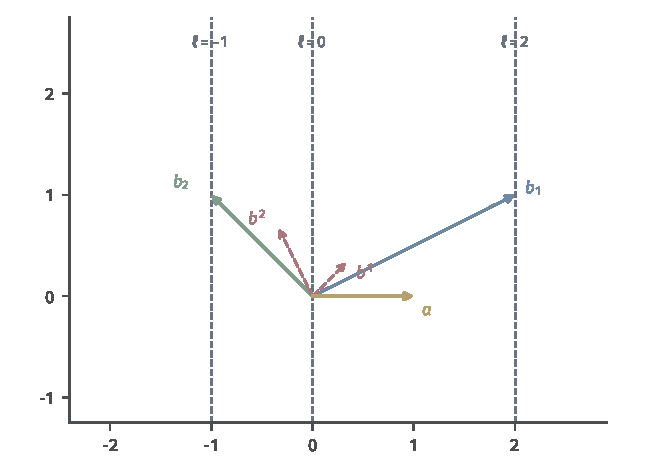
\includegraphics[width=112mm]{figures/00-shared/mathematical-preliminaries-upper/02-linear-spaces/matplotlib/ls-dual-basis-readout/ls-dual-basis-readout.pdf}
  \caption{对偶读取的几何示意。蓝箭头$\bm b_1=(2,1)$、绿箭头$\bm b_2=(-1,1)$为基向量；红色虚线箭头$\bm b^1=(1/3,1/3)$、$\bm b^2=(-1/3,2/3)$分别是对偶基$\varphi_1,\varphi_2$的系数向量，即$\varphi_i(\bm x)=\bm b^i\cdot\bm x$，满足$\varphi_i(\bm b_j)=\delta_{i,j}$。把读取规则画成平面箭头借用了标准内积，这一对应在第~\ref{sec:ls-riesz-representation}节说明。黄色箭头$\bm a=(1,0)$给出读取$\ell(\bm x)=\bm a\cdot\bm x$，灰色虚线为等值线$\ell=c$（$c=-1,0,2$）；$\ell(\bm b_1)=2$、$\ell(\bm b_2)=-1$，且$\bm a=2\bm b^1-\bm b^2$。}
  \label{fig:ls-dual-basis-readout}
\end{figure}

换基时，读取系数与坐标按相反的方向变化。设新基$\mathcal B'$由换基矩阵$\bm P=\bm S_{\mathcal B\leftarrow\mathcal B'}$给出，即$\bm b'_j=\sum_i\bm P_{i,j}\bm b_i$。坐标按
\[
 [\bm v]_{\mathcal B'}=\bm P^{-1}[\bm v]_{\mathcal B}
\]
变化；读取系数则按$\varphi(\bm b'_j)=\sum_i\varphi(\bm b_i)\bm P_{i,j}$变化，即
\[
 [\varphi]_{\mathcal B'}=[\varphi]_{\mathcal B}\bm P.
\]
二者相乘时$\bm P$与$\bm P^{-1}$相消，所以读数$\varphi(\bm v)$不随基改变，这正是读数应有的性质。

% 对偶空间：对偶映射与转置。

\section{对偶映射}
\label{sec:ls-dual-map}

已知线性映射$T:V\to W$和输出端的一个读取$f\in W^*$，输入$\bm x$经过$T$以后被读成$f(T\bm x)$。先作用、再读取，合起来是输入端的一个读取。由这一复合定义\term{对偶映射}（dual map）$T':W^*\to V^*$：
\begin{equation}
\begin{gathered}
T'f=f\circ T\\
(T'f)(\bm x)=f(T\bm x).
\end{gathered}
\label{eq:ls-dual-map-def}
\end{equation}
$T'$保持线性组合：$(T'(\alpha f+\beta g))(\bm x)=\alpha f(T\bm x)+\beta g(T\bm x)$。对象从$V$走到$W$，读取则从$W^*$传回$V^*$，方向相反；这只是把读取规则搬回输入端，不是对$T$求逆。

复合时次序也随之反转：对$S:W\to U$，$(S\circ T)'f=f\circ S\circ T=T'(S'f)$，即$(S\circ T)'=T'\circ S'$。

\paragraph{对偶映射的矩阵是转置}
设$T$在输入基$\mathcal B=(\bm b_1,\ldots,\bm b_d)$、输出基$\mathcal C=(\bm c_1,\ldots,\bm c_m)$下的矩阵为$\bm A$，即$T\bm b_j=\sum_ka_{k,j}\bm c_k$；两组基的对偶基分别记为$\varphi_1,\ldots,\varphi_d$与$\psi_1,\ldots,\psi_m$。取输出读取$f=\sum_iy_i\psi_i$，它传回输入端以后，在输入基向量上的读数是
\[
 (T'f)(\bm b_j)=f(T\bm b_j)
 =\sum_iy_i\,\psi_i\Bigl(\sum_ka_{k,j}\bm c_k\Bigr)
 =\sum_ia_{i,j}y_i=(\bm A^\top\bm y)_j .
\]
上一节说明，读取在对偶基下的坐标就是它在各基向量上的读数，所以$T'f$的坐标为$\bm A^\top\bm y$。也就是说，在对偶基下，对偶映射的矩阵是$\bm A^\top$。转置的乘积规则$(\bm B\bm A)^\top=\bm A^\top\bm B^\top$正是$(S\circ T)'=T'\circ S'$的坐标记录。下面用一个具体映射核对这一结论。
\begin{example}[把输出的第一个分量读取传回输入端]
\label{ex:ls-dual-map-first-component}
再看$T(x_1,x_2)=(2x_1+x_2,\ 3x_2)$，它在标准基下的矩阵为
\[
 \bm A=\begin{bmatrix}2&1\\0&3\end{bmatrix}.
\]
在输出端读取第一个分量，即$f=\psi_1$，系数$\bm y=(1,0)^\top$。按定义先作用再读取，$(T'f)(\bm x)=f(T\bm x)=2x_1+x_2$，传回输入端的读取系数为$(2,1)^\top$。按转置计算，$\bm A^\top(1,0)^\top=(2,1)^\top$，两种算法一致。这组系数正是$\bm A$的第一行：输出的第一个分量本来就由第一行与输入相乘得到。
\end{example}
一般地，读取输出的第$i$个分量并传回输入端，得到的读取系数就是$\bm A$的第$i$行，所以$T'$的像在坐标下就是行空间。

\paragraph{再证行秩等于列秩}
对偶映射给出定理~\ref{thm:ls-row-rank-column-rank}的另一个证明，它不把矩阵分解为两个因子，而是计算$T'$的核。$T'f=0$意味着$f(T\bm x)=0$对一切$\bm x$成立，即$f$在$\operatorname{im}T$上恒为零。所以$\ker T'$由对全部可达输出读数为零的读取组成，在坐标下就是$\bm A^\top\bm y=\bm0$，即左零空间。

下面计算它的维数。设$r=\operatorname{rank}T$，取$\operatorname{im}T$的基$\bm c_1,\ldots,\bm c_r$并扩充为$W$的基$\bm c_1,\ldots,\bm c_m$，对偶基为$\psi_1,\ldots,\psi_m$。读取$f=\sum_iy_i\psi_i$在$\operatorname{im}T$上恒为零，当且仅当它在$\bm c_1,\ldots,\bm c_r$上都读到零，即$y_1=\cdots=y_r=0$。所以$\ker T'=\operatorname{span}\{\psi_{r+1},\ldots,\psi_m\}$，维数为$m-r$。

对$T':W^*\to V^*$用秩零度定理，$\operatorname{rank}T'=\dim W^*-\dim\ker T'=m-(m-r)=r$。$T'$的矩阵是$\bm A^\top$，于是$\operatorname{rank}\bm A^\top=\operatorname{rank}\bm A$。

读取规则至此有了自己的空间、坐标和传递规律。读取的大小，即输入有界时读数最大能有多大，需要先给输入规定范数，由第~\ref{sec:ls-dual-norms}节的对偶范数回答；读取能否写成与某个固定向量的内积，由第~\ref{sec:ls-riesz-representation}节回答。

% 对偶空间：对偶范数。

\section{对偶范数}
\label{sec:ls-dual-norms}

第~\ref{sec:ls-dual-spaces}节的线性泛函是对向量的读取。有了范数，就可以衡量一个读取有多大。误差分析中的典型问题是：误差$\bm r$只知道落在某个范数球内，一次加权读取$\bm z^\top\bm r$最多变化多少。在$\mathbb R^d$上取定一种范数后，这个最大值就是对偶范数。
\begin{definition}[对偶范数]
\label{def:linear-algebra-dual-norm}
给定$\mathbb R^d$上的范数，相对于标准坐标配对的\term{对偶范数}（dual norm）为
\begin{equation}
 \lVert\bm z\rVert_*=\sup_{\lVert\bm r\rVert\leq1}|\bm z^\top\bm r|.
 \label{eq:linear-algebra-dual-norm-definition}
\end{equation}
\end{definition}
这就是第~\ref{sec:ls-matrix-norms}节的诱导范数取输出空间为$\mathbb R$的情形：读取$\bm r\mapsto\bm z^\top\bm r$是$1\times d$矩阵$\bm z^\top$的作用。所以对任意范数，上确界有限并且可以取到。

对偶范数满足范数的各条要求，因而是对偶空间上的范数。非负性显然。$\bm z\neq\bm0$时，取$\bm z$的某个非零坐标$z_j$，则$\bm r=\bm e_j/\lVert\bm e_j\rVert$给出$|\bm z^\top\bm r|=|z_j|/\lVert\bm e_j\rVert>0$，这给出正定性。对每个$\bm r$都有$|(\bm z+\bm w)^\top\bm r|\leq|\bm z^\top\bm r|+|\bm w^\top\bm r|$，取上确界即得三角不等式；齐次性由$|(c\bm z)^\top\bm r|=|c|\,|\bm z^\top\bm r|$得到。图~\ref{fig:ls-dual-norm-unit-ball}把这个最大值画成支撑线最后接触单位球的位置。

\begin{figure}[!htb]
  \centering
  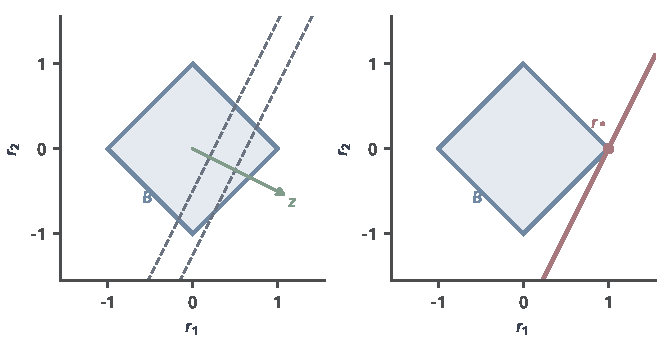
\includegraphics[width=112mm]{figures/00-shared/mathematical-preliminaries-upper/02-linear-spaces/matplotlib/ls-dual-norm-unit-ball/ls-dual-norm-unit-ball.pdf}
  \caption{对偶范数的几何：在原范数单位球$\lVert\bm r\rVert\leq1$上求线性读取$\bm z^\top\bm r$的最大值。左：原单位球（灰色）与读取方向$\bm z$；右：支撑直线最后接触单位球处给出$\lVert\bm z\rVert_*=\max_{\lVert\bm r\rVert\leq1}|\bm z^\top\bm r|$。对偶单位球（虚线）与原单位球互为极体。解析教学例。}
  \label{fig:ls-dual-norm-unit-ball}
\end{figure}

对$\ell_p$范数，对偶范数可以明确写出：
\begin{equation}
(\lVert\cdot\rVert_p)_*=\lVert\cdot\rVert_q,\qquad\frac1p+\frac1q=1.
\label{eq:linear-algebra-lp-duality}
\end{equation}
由齐次性，对任意预算$\rho\geq0$还有
\begin{equation}
 \max_{\lVert\bm r\rVert_p\leq\rho}|\bm z^\top\bm r|
 =\rho\lVert\bm z\rVert_q.
 \label{eq:linear-algebra-linear-perturbation-duality}
\end{equation}
Hölder不等式（定理~\ref{thm:linear-algebra-holder}）给出$\ell_p$单位球上的上界$\lVert\bm z\rVert_q$。这个上界可以达到。$1<p<\infty$且$\bm z\neq\bm0$时，取$r_j=|z_j|^{q-1}\operatorname{sgn}(z_j)/\lVert\bm z\rVert_q^{q-1}$；$\bm z=\bm0$时上界为零，任取可行输入即可。$p=1$时，把单位预算全部放在$|z_j|$最大的坐标上；$p=\infty$时，逐坐标取$r_j=\operatorname{sgn}(z_j)$。下面固定一个读取，比较三种误差预算。
\begin{example}[同一读取在三种误差预算下的最大变化]
\label{ex:ls-dual-norm-three-budgets}
取读取方向$\bm z=(2,-1)^\top$，即读取$\bm z^\top\bm r=2r_1-r_2$，让误差$\bm r$分别落在三种单位球内。

在$\ell_1$单位球上，预算只能分给各坐标的绝对值，全部放在权重$|z_j|$最大的第一个坐标最划算：$\bm r=(1,0)^\top$给出最大值$\lVert\bm z\rVert_\infty=2$。在$\ell_2$单位球上，最坏误差与$\bm z$同方向，取$\bm r=\bm z/\lVert\bm z\rVert_2=(2,-1)^\top/\sqrt5$，最大值为$\lVert\bm z\rVert_2=\sqrt5$。在$\ell_\infty$单位球上，每个坐标都可以同时取满，只需让符号与$z_j$一致：$\bm r=(1,-1)^\top$给出最大值$\lVert\bm z\rVert_1=3$。换成实际的误差预算$|r_j|\leq0.01$，就在式~\eqref{eq:linear-algebra-linear-perturbation-duality}中取$p=\infty$、$\rho=0.01$，最大变化为$0.01\cdot(2+1)=0.03$，由$\bm r=(0.01,-0.01)^\top$达到。

三种单位球给出的最大值依次为$2$、$\sqrt5$、$3$。读取本身没有变，变的是允许误差的形状：它决定了最坏方向在哪里，也决定了读取方向要用哪个对偶范数计量。
\end{example}
图~\ref{fig:linear-algebra-dual-unit-balls}画出这三种情形下的最坏方向。
\begin{figure*}[htbp]
  \centering
  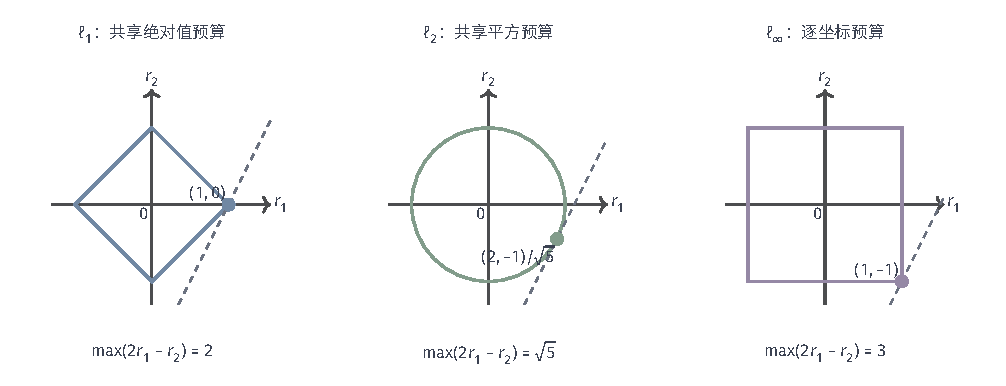
\includegraphics[width=168.998mm]{figures/00-shared/mathematical-preliminaries-upper/02-linear-spaces/tikz/linear-algebra-dual-unit-balls/figure.pdf}
  \caption{同一线性读取$2r_1-r_2$在$\ell_1$、$\ell_2$、$\ell_\infty$单位球上的最大值依次为$2$、$\sqrt5$、$3$。虚线为最后接触可行集的支撑直线，点为最大化方向。三图坐标尺度相同，均为解析教学例；允许误差的形状改变时，误差常数也随之改变。}
  \label{fig:linear-algebra-dual-unit-balls}
\end{figure*}

由此可见，误差预算按$\ell_\infty$给出时，读取方向要按$\ell_1$计量；预算按$\ell_2$给出时，读取方向仍按$\ell_2$计量。

原空间的范数改变，对偶范数随之改变。对加权的坐标范数，可以用换元把问题化回已知情形。
\begin{example}[加权$\ell_1$范数的对偶范数]
\label{ex:ls-weighted-dual-norm}
设权重$w_1,\ldots,w_d>0$，在$\mathbb R^d$上取加权范数$\lVert\bm r\rVert_{\bm w}=\sum_jw_j|r_j|$。把权重吸收进变量，令$s_j=w_jr_j$，则$\lVert\bm r\rVert_{\bm w}=\lVert\bm s\rVert_1$，$\bm z^\top\bm r=\sum_j(z_j/w_j)s_j$。$\bm r$取遍$\lVert\bm r\rVert_{\bm w}\leq1$时，$\bm s$恰好取遍$\ell_1$单位球。由式~\eqref{eq:linear-algebra-lp-duality}中$p=1$的情形，
\[
 \lVert\bm z\rVert_*=\max_j\frac{|z_j|}{w_j}.
\]
仍取上例的$\bm z=(2,-1)^\top$。不加权，即$\bm w=(1,1)^\top$时，$\lVert\bm z\rVert_*=2$，由$\bm r=(1,0)^\top$取到，与上例的$\ell_1$情形一致；改用$\bm w=(4,1)^\top$时，$\lVert\bm z\rVert_*=\max\{1/2,1\}=1$，由$\bm r=(0,-1)^\top$取到。

读取$\bm z^\top\bm r$的代数表达没有变，它的大小却随原空间的范数改变。第一个坐标的权重变大后，同样的预算只允许它有更小的变化，最坏方向因而转到第二个坐标。
\end{example}
所以讨论“输入误差最多引起多大输出误差”时，必须先说清误差用哪种范数度量。内积诱导的范数下，对偶范数等于表示向量的长度，在第~\ref{sec:ls-riesz-representation}节证明。一般有限维空间$V$上的线性泛函$\varphi$同样定义$\lVert\varphi\rVert_*=\max_{\lVert\bm v\rVert\leq1}|\varphi(\bm v)|$，它是取$W=\mathbb R$时的算子范数。无限维空间中，并非每个线性泛函都连续，代数对偶与连续对偶需要区分，这同样属于无限维理论。

% 对偶空间：线性泛函的内积表示。

\section{线性泛函的内积表示}
\phantomsection
\label{sec:ls-riesz-representation}
在$\mathbb R^d$的欧氏内积下，加权读取$\varphi(\bm x)=\bm a^\top\bm x$就是与向量$\bm a$的内积。在一般有限维内积空间中，每个读取也都能这样写。
\begin{theorem}[有限维Riesz表示定理]
\label{thm:ls-riesz-representation}
设$V$是有限维内积空间。对每个$\varphi\in V^*$，存在唯一的$\bm v_\varphi\in V$，使$\varphi(\bm x)=\langle\bm x,\bm v_\varphi\rangle$对所有$\bm x\in V$成立。
\end{theorem}
\begin{proof}
取$V$的一组标准正交基$\bm q_1,\ldots,\bm q_d$（第~\ref{sec:ls-orthonormal-basis-construction}节），令$\bm v_\varphi=\sum_j\varphi(\bm q_j)\bm q_j$。由式~\eqref{eq:ls-orthonormal-expansion}，$\bm x=\sum_j\langle\bm x,\bm q_j\rangle\bm q_j$，于是
\[
 \varphi(\bm x)=\sum_j\langle\bm x,\bm q_j\rangle\varphi(\bm q_j)=\Bigl\langle\bm x,\sum_j\varphi(\bm q_j)\bm q_j\Bigr\rangle=\langle\bm x,\bm v_\varphi\rangle.
\]
若$\bm v,\bm v'$都满足要求，则$\langle\bm x,\bm v-\bm v'\rangle=0$对一切$\bm x$成立，取$\bm x=\bm v-\bm v'$得$\bm v=\bm v'$。
\end{proof}
对应$\varphi\mapsto\bm v_\varphi$保持线性组合，这由表示向量的唯一性得到；每个$\bm v$又都表示读取$\langle\cdot,\bm v\rangle$。所以这个对应是$V^*$到$V$的双射。在它之下，标准正交基的对偶基就是这组基本身，因为第$j$个坐标读取是$\bm x\mapsto\langle\bm x,\bm q_j\rangle$。对一般的基，对偶基对应的向量与原基不同：图~\ref{fig:ls-dual-basis-readout}中的红色箭头$\bm b^1,\bm b^2$，正是对偶读取$\varphi_1,\varphi_2$在欧氏内积下对应的向量。

表示向量依赖内积，读取本身却不依赖。在$\mathbb R^d$上取加权内积$\langle\bm x,\bm y\rangle_{\bm M}=\bm x^\top\bm M\bm y$，同一个读取$\varphi(\bm x)=\bm a^\top\bm x=\bm x^\top\bm M(\bm M^{-1}\bm a)$对应的向量是$\bm M^{-1}\bm a$，而不是$\bm a$。函数空间中也是如此。
\begin{example}[积分读取在两点内积下的表示向量]
\label{ex:ls-riesz-integral-two-point}
在$P_1$上取两点内积$\langle f,g\rangle=f(0)g(0)+f(1)g(1)$，考虑积分读取$\varphi(f)=\int_0^1f(t)\,\mathrm dt$。对$f=a+bt$，$\varphi(f)=a+b/2$。要把它写成与某个固定函数的内积，而这个内积只用到$f(0)=a$与$f(1)=a+b$，所以先把$a+b/2$表示成这两个值的组合：$a+b/2=\tfrac12\bigl(f(0)+f(1)\bigr)$。这正是$f$与常数函数$\tfrac12$的内积：
\[
 \Bigl\langle f,\tfrac12\Bigr\rangle=\tfrac12\bigl(f(0)+f(1)\bigr)=\tfrac12(a+a+b)=a+\frac b2 .
\]

因此$\bm v_\varphi$是常数函数$\tfrac12$。在系数向量的欧氏内积下，同一个读取对应$(1,1/2)^\top$，表示向量随内积而变。等式$\varphi(f)=\tfrac12\bigl(f(0)+f(1)\bigr)$也说明梯形公式对一次函数精确。
\end{example}
表示向量还给出读取的大小。由Cauchy--Schwarz不等式，$|\varphi(\bm x)|\leq\lVert\bm x\rVert\,\lVert\bm v_\varphi\rVert$；$\bm v_\varphi\neq\bm0$时，取$\bm x=\bm v_\varphi/\lVert\bm v_\varphi\rVert$可取到等号。所以仿照第~\ref{sec:ls-dual-norms}节，在单位球上取读取的最大值，得到
\[
 \lVert\varphi\rVert_*=\max_{\lVert\bm x\rVert\leq1}|\varphi(\bm x)|=\lVert\bm v_\varphi\rVert .
\]
在$\mathbb R^d$的欧氏内积下，这就是$\ell_2$范数的对偶范数仍为$\ell_2$范数。

% 对偶空间：伴随与特殊线性算子。

\section{伴随与特殊线性算子}
\label{sec:ls-adjoints}
对偶映射把输出端的读取$f$传回输入端，得到读取$f\circ T$。若把两端的读取都换成表示它的向量，就得到伴随。
\begin{definition}[伴随]
\label{def:linear-algebra-adjoint}
设$T:V\to W$是两个有限维实内积空间之间的线性映射。若存在$T^\star:W\to V$使
\begin{equation}
 \langle T\bm x,\bm y\rangle_W=\langle\bm x,T^\star\bm y\rangle_V
 \label{eq:ls-adjoint-pairing}
\end{equation}
对所有$\bm x\in V$、$\bm y\in W$成立，则$T^\star$称为$T$的\term{伴随}（adjoint）。
\end{definition}

伴随总存在且唯一。固定$\bm y\in W$，$\bm x\mapsto\langle T\bm x,\bm y\rangle_W$是$V$上的线性泛函。由定理~\ref{thm:ls-riesz-representation}，存在唯一的向量使它写成与该向量的内积，把这个向量记为$T^\star\bm y$。$T^\star$对$\bm y$线性：
\[
 \langle\bm x,aT^\star\bm y+bT^\star\bm y'\rangle_V=a\langle T\bm x,\bm y\rangle_W+b\langle T\bm x,\bm y'\rangle_W=\langle T\bm x,a\bm y+b\bm y'\rangle_W,
\]
由表示向量的唯一性，$T^\star(a\bm y+b\bm y')=aT^\star\bm y+bT^\star\bm y'$。

用对偶映射的语言说，把$\bm y\in W$看成读取$\langle\cdot,\bm y\rangle_W$，则$T'$把它送到读取$\langle T\,\cdot,\bm y\rangle_W=\langle\cdot,T^\star\bm y\rangle_V$。所以伴随就是借内积把读取换成向量以后的对偶映射。

具体计算时，取$V,W$的基。由坐标下的内积公式，两边的内积写成$\langle\bm x,\bm x'\rangle_V=\bm x^\top\bm M_V\bm x'$、$\langle\bm y,\bm y'\rangle_W=\bm y^\top\bm M_W\bm y'$，这里$\bm x,\bm y$等指坐标，$\bm M_V,\bm M_W$是两组基的Gram矩阵，对称正定因而可逆。设$T$的矩阵为$\bm A$，伴随的矩阵为$\bm B$。式~\eqref{eq:ls-adjoint-pairing}要求$(\bm A\bm x)^\top\bm M_W\bm y=\bm x^\top\bm M_V\bm B\bm y$对所有$\bm x,\bm y$成立。取$\bm x,\bm y$为标准坐标向量逐个比较元素，这等价于$\bm A^\top\bm M_W=\bm M_V\bm B$，即
\begin{equation}
 \bm B=\bm M_V^{-1}\bm A^\top\bm M_W.
 \label{eq:ls-weighted-adjoint}
\end{equation}
两端都取标准正交基时，$\bm M_V,\bm M_W$都是单位矩阵，伴随矩阵就是$\bm A^\top$，与对偶映射的矩阵相同。一般情形下，伴随既不是单纯转置，也不是转置再求逆。下面的例子说明这一点。
\begin{example}[加权内积下的伴随]
\label{ex:ls-weighted-adjoint}
设$V=W=\mathbb R^2$都取加权内积$\langle\bm x,\bm y\rangle_{\bm M}=\bm x^\top\bm M\bm y$，$\bm M=\operatorname{diag}(4,1)$，并考虑把第二个坐标移到第一个位置的映射$T\bm x=\bm A\bm x$，其中
\[
 \bm A=\begin{bmatrix}0&1\\0&0\end{bmatrix}.
\]
标准基在这个内积下不是标准正交基，所以伴随要用式~\eqref{eq:ls-weighted-adjoint}计算：
\[
 \bm B=\bm M^{-1}\bm A^\top\bm M
 =\begin{bmatrix}1/4&0\\0&1\end{bmatrix}\begin{bmatrix}0&0\\1&0\end{bmatrix}\begin{bmatrix}4&0\\0&1\end{bmatrix}
 =\begin{bmatrix}0&0\\4&0\end{bmatrix}.
\]
再回到配对等式核对：$\bm A\bm x=(x_2,0)^\top$，$\langle\bm A\bm x,\bm y\rangle_{\bm M}=4x_2y_1$；$\bm B\bm y=(0,4y_1)^\top$，$\langle\bm x,\bm B\bm y\rangle_{\bm M}=x_2\cdot4y_1$，两者相等。因数$4$来自输出落在权重为$4$的第一个坐标上，伴随要把这个权重带回输入端。所以伴随矩阵是$\bm B$，而不是$\bm A^\top$：
\[
 \bm B=\begin{bmatrix}0&0\\4&0\end{bmatrix}\neq\begin{bmatrix}0&0\\1&0\end{bmatrix}=\bm A^\top.
\]
\end{example}
对偶映射的矩阵总是$\bm A^\top$；伴随与它的差别，来自读取与向量之间的对应$\bm a\mapsto\bm M^{-1}\bm a$随内积改变。四个基本子空间正交关系的证明只用到配对恒等式，所以在一般内积空间中同样有$\ker T^\star=(\operatorname{im}T)^\perp$、$\ker T=(\operatorname{im}T^\star)^\perp$。

\paragraph{伴随的运算规则}
由配对定义可以逐条推出伴随的运算规则：
\[
 \begin{gathered}
(T+S)^\star=T^\star+S^\star,\\
(cT)^\star=c\,T^\star,\\
(TS)^\star=S^\star T^\star,\\
T^{\star\star}=T.
 \end{gathered}
\]
例如$\langle TS\bm x,\bm y\rangle=\langle S\bm x,T^\star\bm y\rangle=\langle\bm x,S^\star T^\star\bm y\rangle$，复合的伴随与乘积的转置一样反转次序；恒等映射的伴随是自身。图~\ref{fig:ls-adjoint-action-transfer}画出伴随怎样把配对从输出端搬回输入端。

伴随不是逆：逆把输出复原成输入，伴随只把作用从内积的一侧移到另一侧。
\begin{example}[反例：伴随不是逆]
\label{ex:ls-adjoint-not-inverse}
最简单的反例是非零内积空间$V$上的放大两倍$T=2\operatorname{id}$。数乘可以从内积的一侧移到另一侧，$\langle2\bm x,\bm y\rangle=\langle\bm x,2\bm y\rangle$对一切$\bm x,\bm y$成立，所以$T^\star=2\operatorname{id}$：伴随仍是放大两倍。复原输入的逆却是缩小一半，$T^{-1}=\tfrac12\operatorname{id}$。因此$T^\star\neq T^{-1}$。两者相等恰好是正交算子的条件，下面马上会遇到。
\end{example}
\begin{figure}[!htb]
  \centering
  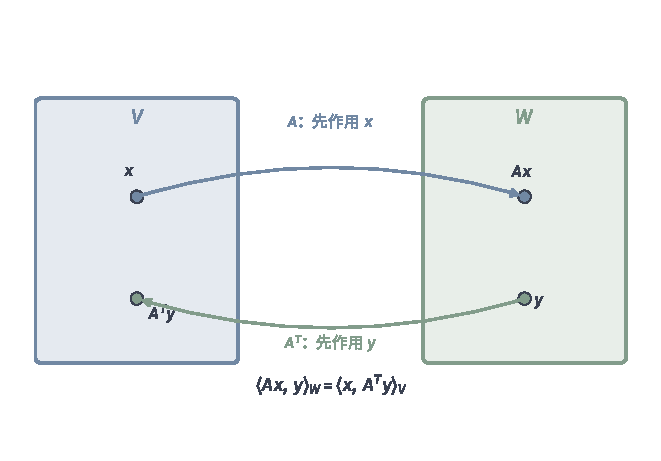
\includegraphics[width=112mm]{figures/00-shared/mathematical-preliminaries-upper/02-linear-spaces/matplotlib/ls-adjoint-action-transfer/ls-adjoint-action-transfer.pdf}
  \caption{内积伴随把输出端的配对搬回输入端。左：$T:V\to W$把$\bm x$映成$T\bm x$，与$\bm y\in W$配对；右：伴随$T^\star:W\to V$把$\bm y$映回$T^\star\bm y\in V$，使$\langle T\bm x,\bm y\rangle_W=\langle\bm x,T^\star\bm y\rangle_V$。标准欧氏内积下$T^\star$就是转置；它反转的是配对的方向，不是逆作用。箭头与空间为解析示意。}
  \label{fig:ls-adjoint-action-transfer}
\end{figure}

\paragraph{自伴、正交与正规算子}
对算子$T:V\to V$，伴随仍是$V$上的算子，可以与$T$比较。下面四类算子都由$T$与$T^\star$之间的一个等式规定。

若$T^\star=T$，称$T$为\term{自伴}（self-adjoint）算子，它在标准正交基下对应对称矩阵。若$T^\star=-T$，称$T$为\term{反自伴}（skew-adjoint）算子，它在标准正交基下对应满足$\bm A^\top=-\bm A$的反对称矩阵。反自伴算子把每个向量送到与它正交的方向：由$\langle T\bm x,\bm x\rangle=\langle\bm x,T^\star\bm x\rangle=-\langle\bm x,T\bm x\rangle$得$\langle T\bm x,\bm x\rangle=0$。例如平面上的$\left[\begin{smallmatrix}0&-1\\1&0\end{smallmatrix}\right]$把$(x_1,x_2)^\top$送到$(-x_2,x_1)^\top$，即逆时针旋转直角。

若$Q^\star Q=\operatorname{id}$，则$Q$保持内积：$\langle Q\bm x,Q\bm y\rangle=\langle\bm x,Q^\star Q\bm y\rangle=\langle\bm x,\bm y\rangle$，称为正交算子。它在标准正交基下对应第~\ref{sec:ls-orthogonal-matrices}节的正交矩阵；由方阵的单侧逆即双侧逆，$Q^{-1}=Q^\star$。

满足$TT^\star=T^\star T$的算子称为\term{正规}（normal）算子，即$T$与自己的伴随可交换。自伴、反自伴与正交算子都是正规算子：前两种情形$T^\star=\pm T$显然与$T$交换，正交算子满足$QQ^\star=Q^\star Q=\operatorname{id}$。一般算子未必正规，例如示例~\ref{ex:ls-weighted-adjoint}中的$\bm A=\left[\begin{smallmatrix}0&1\\0&0\end{smallmatrix}\right]$在欧氏内积下满足$\bm A\bm A^\top=\operatorname{diag}(1,0)\neq\operatorname{diag}(0,1)=\bm A^\top\bm A$。这些算子的谱性质在第~\ref{chap:eigen-spectral-decomposition}章讨论，这里只给出定义。

\paragraph{复空间中的泛函表示与伴随}
复空间沿用前面“第一变量共轭线性、第二变量线性”的约定。这时线性泛函应写成$\varphi(\bm x)=\langle\bm v,\bm x\rangle$，让$\bm x$处于线性的变量位置。若$\bm q_1,\ldots,\bm q_d$是标准正交基，则$\bm v=\sum_j\overline{\varphi(\bm q_j)}\bm q_j$；代入各基向量即可核对读数。表示向量随泛函作共轭线性变化，这与实空间中的线性对应不同。

例如在$\mathbb C$的标准内积$\langle v,z\rangle=\overline v z$下，泛函$\varphi(z)=(1+\mathrm i)z$对应$v=1-\mathrm i$，因为$\overline v z=(1+\mathrm i)z$。若交换两个变量的位置，得到的表达式关于$z$共轭线性，不再是线性泛函。所以共轭来自内积约定，不能从实数公式中直接删去。

两个复内积空间之间的伴随仍由$\langle T\bm x,\bm y\rangle_W=\langle\bm x,T^\star\bm y\rangle_V$定义。在标准正交基下，若$T$的矩阵为$\bm A$，伴随的矩阵就是$\bm A^*$；若两端基的Gram矩阵为$\bm M_V,\bm M_W$，则为$\bm M_V^{-1}\bm A^*\bm M_W$。这与代数对偶映射的矩阵$\bm A^\top$不同：后者只复合线性泛函，不涉及内积和共轭。复空间中，自伴矩阵满足$\bm A=\bm A^*$；保持内积的方阵满足$\bm A^*\bm A=\bm I$，称为酉矩阵。

\section{本章小结}
\label{sec:ls-dual-spaces-summary}

本章回答了章首的三个问题：线性读取组成对偶空间，读取经对偶映射在两端之间传递，读取的大小由对偶范数度量。

对偶空间由线性泛函组成，维数与原空间相同；对偶基就是坐标读取，用对偶基表示一个读取时不必解方程。对偶映射把输出端的读取传回输入端，在对偶基下记录为转置，由此又得到行秩等于列秩。这些结论只用线性运算，与范数和内积无关。

有了范数，读取就有了大小。对偶范数是读取在单位球上的最大绝对值，也就是误差受限时读取的最大变化；$\ell_p$范数的对偶范数是$\ell_q$范数，$1/p+1/q=1$，最坏方向由Hölder不等式的取等条件给出。讨论“输入误差最多引起多大输出误差”时，必须先说明误差用哪种范数度量。

有了内积，读取又可以写成向量。Riesz表示定理说明，有限维内积空间上的每个线性泛函都是与唯一一个向量的内积，内积诱导范数下对偶范数就是这个向量的长度。把对偶映射两端的读取都换成向量，就得到伴随：在标准正交基下伴随就是转置，在一般基下还要计入两端的Gram矩阵。自伴、正交与正规算子都由伴随定义，第~\ref{chap:eigen-spectral-decomposition}章的谱定理将在这类算子上展开。


